\documentclass[]{book}
\usepackage{lmodern}
\usepackage{amssymb,amsmath}
\usepackage{ifxetex,ifluatex}
\usepackage{fixltx2e} % provides \textsubscript
\ifnum 0\ifxetex 1\fi\ifluatex 1\fi=0 % if pdftex
  \usepackage[T1]{fontenc}
  \usepackage[utf8]{inputenc}
\else % if luatex or xelatex
  \ifxetex
    \usepackage{mathspec}
  \else
    \usepackage{fontspec}
  \fi
  \defaultfontfeatures{Ligatures=TeX,Scale=MatchLowercase}
\fi
% use upquote if available, for straight quotes in verbatim environments
\IfFileExists{upquote.sty}{\usepackage{upquote}}{}
% use microtype if available
\IfFileExists{microtype.sty}{%
\usepackage{microtype}
\UseMicrotypeSet[protrusion]{basicmath} % disable protrusion for tt fonts
}{}
\usepackage{hyperref}
\hypersetup{unicode=true,
            pdftitle={Modelización en R},
            pdfauthor={Aula Innova. Innova-tsn},
            pdfborder={0 0 0},
            breaklinks=true}
\urlstyle{same}  % don't use monospace font for urls
\usepackage{color}
\usepackage{fancyvrb}
\newcommand{\VerbBar}{|}
\newcommand{\VERB}{\Verb[commandchars=\\\{\}]}
\DefineVerbatimEnvironment{Highlighting}{Verbatim}{commandchars=\\\{\}}
% Add ',fontsize=\small' for more characters per line
\usepackage{framed}
\definecolor{shadecolor}{RGB}{248,248,248}
\newenvironment{Shaded}{\begin{snugshade}}{\end{snugshade}}
\newcommand{\AlertTok}[1]{\textcolor[rgb]{0.94,0.16,0.16}{#1}}
\newcommand{\AnnotationTok}[1]{\textcolor[rgb]{0.56,0.35,0.01}{\textbf{\textit{#1}}}}
\newcommand{\AttributeTok}[1]{\textcolor[rgb]{0.77,0.63,0.00}{#1}}
\newcommand{\BaseNTok}[1]{\textcolor[rgb]{0.00,0.00,0.81}{#1}}
\newcommand{\BuiltInTok}[1]{#1}
\newcommand{\CharTok}[1]{\textcolor[rgb]{0.31,0.60,0.02}{#1}}
\newcommand{\CommentTok}[1]{\textcolor[rgb]{0.56,0.35,0.01}{\textit{#1}}}
\newcommand{\CommentVarTok}[1]{\textcolor[rgb]{0.56,0.35,0.01}{\textbf{\textit{#1}}}}
\newcommand{\ConstantTok}[1]{\textcolor[rgb]{0.00,0.00,0.00}{#1}}
\newcommand{\ControlFlowTok}[1]{\textcolor[rgb]{0.13,0.29,0.53}{\textbf{#1}}}
\newcommand{\DataTypeTok}[1]{\textcolor[rgb]{0.13,0.29,0.53}{#1}}
\newcommand{\DecValTok}[1]{\textcolor[rgb]{0.00,0.00,0.81}{#1}}
\newcommand{\DocumentationTok}[1]{\textcolor[rgb]{0.56,0.35,0.01}{\textbf{\textit{#1}}}}
\newcommand{\ErrorTok}[1]{\textcolor[rgb]{0.64,0.00,0.00}{\textbf{#1}}}
\newcommand{\ExtensionTok}[1]{#1}
\newcommand{\FloatTok}[1]{\textcolor[rgb]{0.00,0.00,0.81}{#1}}
\newcommand{\FunctionTok}[1]{\textcolor[rgb]{0.00,0.00,0.00}{#1}}
\newcommand{\ImportTok}[1]{#1}
\newcommand{\InformationTok}[1]{\textcolor[rgb]{0.56,0.35,0.01}{\textbf{\textit{#1}}}}
\newcommand{\KeywordTok}[1]{\textcolor[rgb]{0.13,0.29,0.53}{\textbf{#1}}}
\newcommand{\NormalTok}[1]{#1}
\newcommand{\OperatorTok}[1]{\textcolor[rgb]{0.81,0.36,0.00}{\textbf{#1}}}
\newcommand{\OtherTok}[1]{\textcolor[rgb]{0.56,0.35,0.01}{#1}}
\newcommand{\PreprocessorTok}[1]{\textcolor[rgb]{0.56,0.35,0.01}{\textit{#1}}}
\newcommand{\RegionMarkerTok}[1]{#1}
\newcommand{\SpecialCharTok}[1]{\textcolor[rgb]{0.00,0.00,0.00}{#1}}
\newcommand{\SpecialStringTok}[1]{\textcolor[rgb]{0.31,0.60,0.02}{#1}}
\newcommand{\StringTok}[1]{\textcolor[rgb]{0.31,0.60,0.02}{#1}}
\newcommand{\VariableTok}[1]{\textcolor[rgb]{0.00,0.00,0.00}{#1}}
\newcommand{\VerbatimStringTok}[1]{\textcolor[rgb]{0.31,0.60,0.02}{#1}}
\newcommand{\WarningTok}[1]{\textcolor[rgb]{0.56,0.35,0.01}{\textbf{\textit{#1}}}}
\usepackage{longtable,booktabs}
\usepackage{graphicx,grffile}
\makeatletter
\def\maxwidth{\ifdim\Gin@nat@width>\linewidth\linewidth\else\Gin@nat@width\fi}
\def\maxheight{\ifdim\Gin@nat@height>\textheight\textheight\else\Gin@nat@height\fi}
\makeatother
% Scale images if necessary, so that they will not overflow the page
% margins by default, and it is still possible to overwrite the defaults
% using explicit options in \includegraphics[width, height, ...]{}
\setkeys{Gin}{width=\maxwidth,height=\maxheight,keepaspectratio}
\IfFileExists{parskip.sty}{%
\usepackage{parskip}
}{% else
\setlength{\parindent}{0pt}
\setlength{\parskip}{6pt plus 2pt minus 1pt}
}
\setlength{\emergencystretch}{3em}  % prevent overfull lines
\providecommand{\tightlist}{%
  \setlength{\itemsep}{0pt}\setlength{\parskip}{0pt}}
\setcounter{secnumdepth}{5}
% Redefines (sub)paragraphs to behave more like sections
\ifx\paragraph\undefined\else
\let\oldparagraph\paragraph
\renewcommand{\paragraph}[1]{\oldparagraph{#1}\mbox{}}
\fi
\ifx\subparagraph\undefined\else
\let\oldsubparagraph\subparagraph
\renewcommand{\subparagraph}[1]{\oldsubparagraph{#1}\mbox{}}
\fi

%%% Use protect on footnotes to avoid problems with footnotes in titles
\let\rmarkdownfootnote\footnote%
\def\footnote{\protect\rmarkdownfootnote}

%%% Change title format to be more compact
\usepackage{titling}

% Create subtitle command for use in maketitle
\providecommand{\subtitle}[1]{
  \posttitle{
    \begin{center}\large#1\end{center}
    }
}

\setlength{\droptitle}{-2em}

  \title{Modelización en R}
    \pretitle{\vspace{\droptitle}\centering\huge}
  \posttitle{\par}
    \author{Aula Innova. Innova-tsn}
    \preauthor{\centering\large\emph}
  \postauthor{\par}
      \predate{\centering\large\emph}
  \postdate{\par}
    \date{Sabadell. Enero-Febrero, 2018}


\begin{document}
\maketitle

{
\setcounter{tocdepth}{1}
\tableofcontents
}
\hypertarget{presentacion}{%
\chapter*{Presentación}\label{presentacion}}
\addcontentsline{toc}{chapter}{Presentación}


\includegraphics[width=0.75\linewidth]{C:/Users/romy.rodriguez/Documents/INNOVA/Formacion/MiCurso/ModelizacionR/imgs/sabadellcurso}

\textbf{Modelización con R} es un manual práctico para la creación y utilización de modelos analíticos con el lenguaje R (R Core Team \protect\hyperlink{ref-R-base}{2017}). En particular, esta versión del manual ha sido desarrollada para el equipo de \emph{modelling} del \textbf{Banc Sabadell} en Barcelona.

El objetivo de este manual es presentar de manera resumida, los principales algoritmos del \emph{analytics}, destacando cuándo deben ser utilizados y cómo evaluar su performance.

Cada capítulo corresponde a un tópico. Se pueden leer de manera individual. Todos los ejemplo están desarrollados con datos incluidos en las librerias de R y/o se encuentran disponibles en la web.

Para realizar las prácticas sugeridas en este manual, el lector requiere un portátil donde tenga instaladas las últimas versiones de R y RStudio. Además debe contar con una conexión a internet y la posibilidad de instalar las librerías que se citan a lo largo del documento.

\hypertarget{part-modelos-analiticos}{%
\part{MODELOS ANALÍTICOS}\label{part-modelos-analiticos}}

\hypertarget{modelizacion}{%
\chapter{Modelizar}\label{modelizacion}}

Los sistemas analíticos están presentes en todas las áreas de negocio del sector bancario. A muy alto nivel, se puede contar con modelos predictivos en la gestión de clientes, gestión del riesgo y en el soporte a las operaciones. Así mismo, dichos sistemas pueden estar desagregados por segmento, producto, región geográfica, etc.

Algunas de las aplicaciones de la modelización son:

\textbf{Clientes}

\begin{itemize}
\tightlist
\item
  Con modelos predictivos se puede mejorar la relación con los clientes, a través de: Anticipación de la Fuga (\textbf{Retención}), Incentivo del Uso de Productos (\textbf{Fidelización}), Adquisición de Nuevos Productos (\textbf{Venta Cruzada}), Anticipación de la Reclamación (\textbf{Satisfacción}), Promociones que le interesen (\textbf{Gestión de Campañas}), etc.
\end{itemize}

\textbf{Riesgo}

\begin{itemize}
\tightlist
\item
  Con modelos analíticos se puede optimizar todo el ciclo de cobranza: Concesión de \textbf{créditos}, Anticipar \textbf{impagos}, Detectar \textbf{fraude}, Optimización de la \textbf{Cobranza}, etc.
\end{itemize}

\textbf{Operaciones}

\begin{itemize}
\tightlist
\item
  Con modelos predictivos se puede hacer más eficientes algunos procesos como: Gestión de \textbf{sucursales}, Optimización de \textbf{personal}, Gestión de \textbf{cajeros} automáticos, Inversión en \textbf{marketing}, Gestión del \textbf{call center}, etc.
\end{itemize}

Las técnicas/modelos analíticos utilizadas dependen del output o target. En general, se trabaja con \textbf{outputs binarios} (1-0), \textbf{outputs continuos} o, más recientemente, \textbf{datos no estructurados}.

\hypertarget{modelizar}{%
\section{¿Qué es Modelizar?}\label{modelizar}}

\textbf{Modelizar} es el proceso de crear, desarrollar y validar modelos que sirvan para convertir los datos en información de negocio significativa que ayude a ejecutar las estrategias y mejorar el rendimiento.

\begin{quote}
\emph{Data science} es la disciplina que permite convertir los \textbf{datos} en \textbf{conocimiento} (Garrett Grolemund \protect\hyperlink{ref-rdc2017}{2017}). \textbf{Modelizar} es una de las fases del \emph{Data Science}.
\end{quote}

Un esquema aceptado sobre las fases de un proyecto de \emph{Data Science} es\footnote{Fuente: \url{http://r4ds.had.co.nz/introduction.html}}:

\begin{quote}
\emph{Data} y \emph{Analytics} van de la mano.
\end{quote}

Más generalmente, como lo expone Marr (\protect\hyperlink{ref-mar2015}{2017}), en el context de \emph{Big Data}, \textbf{apply analytics} (A), se encuentra en el corazón de la estrategia para crear \emph{SMART Business} y aprovechar al máximo el valor de los datos.

En resumen, \textbf{Modelizar} es el proceso de crear, desarrollar y validar modelos que sirvan para convertir los datos en información de negocio significativa que ayude a ejecutar las estrategias y mejorar el rendimiento.

Los modelos más comunes son: modelos de \textbf{regresión}, modelos de \textbf{series temporales}, técnicas de \textbf{machine learning}, etc.

\hypertarget{que-es-un-modelo-analitico}{%
\section{¿Qué es un modelo analítico?}\label{que-es-un-modelo-analitico}}

Un \textbf{modelo} es resumen simple, de baja dimensión, de un conjunto de datos (Garrett Grolemund \protect\hyperlink{ref-rdc2017}{2017}).

Algunas de las afirmaciones tradicionalmente aceptadas sobre un modelo analítico son:

\begin{itemize}
\tightlist
\item
  Un modelo es una representación simplificada de la realidad.
\item
  Un modelo es una forma matemática de describir la relación entre una variable de respuesta y un conjunto de variables independientes.
\item
  Un modelo se puede ver como: (a) Una teoría sobre cómo se generaron los datos y (b) Una forma útil de resumir los datos.
\item
  A un modelo no se le exige que sea \emph{verdadero}, sino que sea \emph{útil}, de acuerdo a los objetivos para los cuales fue creado.
\item
  Todos los modelos son errados, pero algunos son útiles.
\end{itemize}

De manera general, un modelo es una representación del mecanismo generador de los datos. Por ello, un modelo puede verse como un \textbf{resumen de la información disponible} y en consecuencia permite compactar los datos existentes. Los modelos se utilizan principalmente para entender dinámicas del mercado, prever el futuro, simular consecuencias ante cambios, evaluar acciones pasadas, etc.

Los modelos son el elemento central de la creación de inteligencia corporativa.
Condesan y operacionalizan la información existente. Son almacenes y fábricas de conocimiento.

Cuando se quiere hacer uso de un modelo, se suele identificar:

\begin{itemize}
\tightlist
\item
  \emph{output} : variable dependiente, variable respuesta, variable objetivo.
\item
  \emph{input(s)} : variable(s) independiente(s), predictor(es), o simplemente feature(s).
\end{itemize}

\hypertarget{tipos-de-problemas}{%
\chapter{Tipos de Problemas}\label{tipos-de-problemas}}

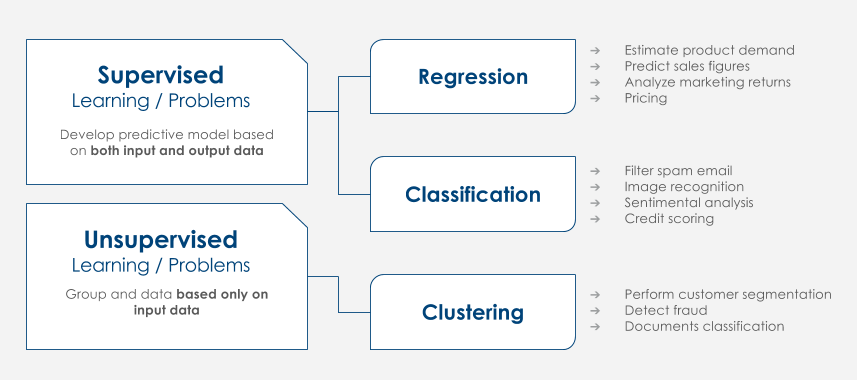
\includegraphics[width=0.9\linewidth]{imgs/mlalgorithms01}

En bastante común que los algoritmos de \emph{Machine Learning} en aprendizaje supervisado y aprendizaje no supervisado. Esta misma clasificación se menciona en la sección \ref{clasemodelos}, las herramientas de \emph{statistical learning}. Este tipo de clasificación responde al tipo de problema e información que disponemos del \emph{output}, por ello, en este Manual generalizamos esta clasificación y la denominamos \textbf{Tipo de Problema Analítico} que debemos afrontar.

\textbf{Problema / Aprendizaje Supervisado}

En el \textbf{aprendizaje supervisado}, cada dato, unidad analizada u observación está etiquetada o asociada con una categoría o valor de interés. Ejemplos:

\begin{itemize}
\tightlist
\item
  Una imagen es etiquetada como un `gato' o `perro'.
\item
  Un cliente es etiquetado como `propenso' o `no propenso' al uso del canal digital.
\item
  El precio de venta asociado a un coche usado, es una etiqueta de valor.
\end{itemize}

El objetivo del aprendizaje supervisado es estudiar muchos ejemplos etiquetados y, luego, poder realizar predicciones sobre los datos futuros. Por ejemplo, identificar nuevas fotografías con el animal correcto, identificar clientes a clientes facilitar el uso de la banca online o asignar precios de venta precisos a otros coches usados.

El aprendizaje supervisado usa técnicas de \textbf{clasificación} y \textbf{regresión} para desarrollar modelos predictivos.

\begin{itemize}
\item
  Las técnicas de \textbf{clasificación} predicen \textbf{respuestas discretas} ---por ejemplo, saber si un correo es genuino o \emph{spam}, o si un tumor es benigno o maligno. Los modelos de clasificación categorizan los datos de entrada. Entre las aplicaciones típicas se incluyen imágenes médicas, reconocimiento de voz o puntaje crediticio. Cuando hay sólo dos opciones, se denomina clasificación de dos clases o binaria. Cundo hay más categorías, se denomina clasificación multiclase o multinomial.

  \begin{itemize}
  \tightlist
  \item
    En algunos casos la \textbf{detección de anomalías} se considera una técnica adicional de clasificación. En la detección de fraude, por ejemplo, los patrones de gasto de tarjeta de crédito muy poco habituales son sospechosos. Las posibles variaciones son tan numerosas y los ejemplos de formación son tan pocos, que no es posible saber de qué actividad fraudulenta se trata. El enfoque que toma la detección de anomalías es simplemente
    aprender qué puede considerarse como actividad normal (haciendo uso de las transacciones no fraudulentas del historial) e identificar todo lo que sea significativamente diferente\footnote{Fuente:\url{https://docs.microsoft.com/es-es/azure/machine-learning/studio/algorithm-choice}}.
  \end{itemize}
\item
  Las técnicas de \textbf{reducción de dimensionalidad } ayudan a disminuir la complejidad de los problemas debida al gran volumen de datos. Cuando mayor es el conjunto de datos, mayor la necesidad de reducir el número de variables (\emph{features}) que se quieren analizar.
\item
  Las técnicas de \textbf{regresión} predicen \textbf{respuestas continuas} ---por ejemplo, cambios en la temperatura o fluctuaciones en la demanda de energía. Las aplicaciones típicas pueden ser previsión del recurso eléctrico o trading algorítmico.
\end{itemize}

\textbf{Problema / Aprendizaje No Supervisado}

En el \textbf{aprendizaje no supervisado}, los datos no tienen etiquetas asociadas a ellos. En este caso, el objetivo es organizar los datos de alguna manera o describir su estructura. Esto puede significar agrupar clientes en segmentos, o buscar diferentes maneras de examinar datos complejos para que parezcan más simples.

El aprendizaje no supervisado se utiliza en análisis exploratorio de datos para encontrar características ocultas y agrupar. Las aplicaciones del clustering incluyen análisis de secuencias genéticas, investigación de mercado y reconocimiento de objetos.

\hypertarget{clasemodelos}{%
\section{Enfoques de Modelización}\label{clasemodelos}}

\emph{Statistical Learning} se refiere a un conjunto de herramientas para modelar y comprender conjuntos de datos complejos.

\emph{Statistical Learning} es un término presentado en Gareth James (\protect\hyperlink{ref-isl2014}{2014}). Hace referencia a un área de reciente desarrollo en estadística, que se combina con desarrollos paralelos de ciencias de la computación (específicamente, \emph{Machine Learning}). Se refiere a un ámplio conjunto de herramientas para \textbf{entender datos}. Estas herramientas pueden ser: \textbf{supervisadas} o \textbf{no supervisadas}. De manera muy genérica, en los problemas supervisados se busca estimar o prever un \emph{output} basado en uno o más \emph{inputs}. En los problemas no supervisados, se cuenta con los \emph{inputs} pero con un \emph{output}, por lo que se busca entender la estructura de los datos.

Otra forma de clasificar los métodos para modelizar se basa en su objetivo y forma de construcción. Cuando se prioriza la \textbf{interpretación del modelo}, buscando que expliquen las relaciones entre \emph{output} e \emph{inputs}, se habla de \textbf{modelos estadísticos}. Cuando se prioriza la \textbf{precisión de la previsión} se habla de algoritmos de \textbf{machine learning}.

Tipos de modelos analíticos: \emph{Modelos Estadísticos} y \emph{Machine Learning}\footnote{Fuente: \url{http://www.kdnuggets.com/2016/11/machine-learning-vs-statistics.html}}. Los primeros hacen uso de la probabilidad (inferencia), son explicativos y predictivos. Los segundos suelen ser `cajas negras', se centran en la previsión y el trabajo con grandes volúmenes de datos\footnote{Ver \url{https://www.quora.com/What-is-the-difference-between-statistics-and-machine-learning}}.

El objetivo de los modelos o algoritmos de \textbf{Machine Learning} es enseñar a las computadoras a hacer lo que es natural para humanos y animales: \textbf{aprender de la experiencia}. Estos algoritmos utilizan métodos computacionales para ``aprender'' información directamente de los datos, sin depender de una ecuación predeterminada como modelo. Los algoritmos mejoran su rendimientode forma adaptativa conforme aumenta la cantidad de muestras (datos) disponibles
para el aprendizaje.

\textbf{Machine Learning}

El \emph{Machine Learning} no requiere hipótesis previas sobre las relaciones subyacentes entre las variables (o inputs). Sólo se deben ingresar todos los datos que se diponga, y el algoritmo procesa los datos y descubre patrones, con los cuales puede hacer predicciones sobre el nuevo conjunto de datos. El aprendizaje automático trata un algoritmo como una \textbf{black box} (caja negra), siempre que funcione. En otras palabras, su principal objetivo es la previsión.

\textbf{Modelos Estadísticos}

Por el contrario, los \textbf{estadísticos} deben comprender cómo se recopilaron los datos, las propiedades estadísticas de los estimadores, la distribución subyacente de la población que están estudiando y los tipos de propiedades que esperaría si hiciera el experimento muchas veces. Necesita saber exactamente lo que está haciendo y proponer parámetros que le proporcionen el poder predictivo.

\hypertarget{catalogo-de-tecnicas}{%
\chapter{Catálogo de Técnicas}\label{catalogo-de-tecnicas}}

\textbf{¿Tus datos pueden ser etiquetados o categorizados?}

Si tus datos pueden ser separados en clases o grupos específicos, usa algoritmos de clasificación.

\textbf{¿Estás trabajando con datos de un rango?}

Si la naturaleza de tu respuesta es un número real - como la temperatura o el tiempo hasta que un cajero automático falle -, usa modelos o algoritmos de regresión.

\textbf{¿Aún no sabes como agrupar tus datos:}

\begin{itemize}
\tightlist
\item
  Usa clúster jerárquico para encontrar posibles estructuras en los datos.
\item
  Usa la evaluación de clústers para encontrar el `mejor' número de grupos.
\end{itemize}

\hypertarget{tecnicas-de-clustering}{%
\section{\texorpdfstring{Técnicas de \emph{Clustering}}{Técnicas de Clustering}}\label{tecnicas-de-clustering}}

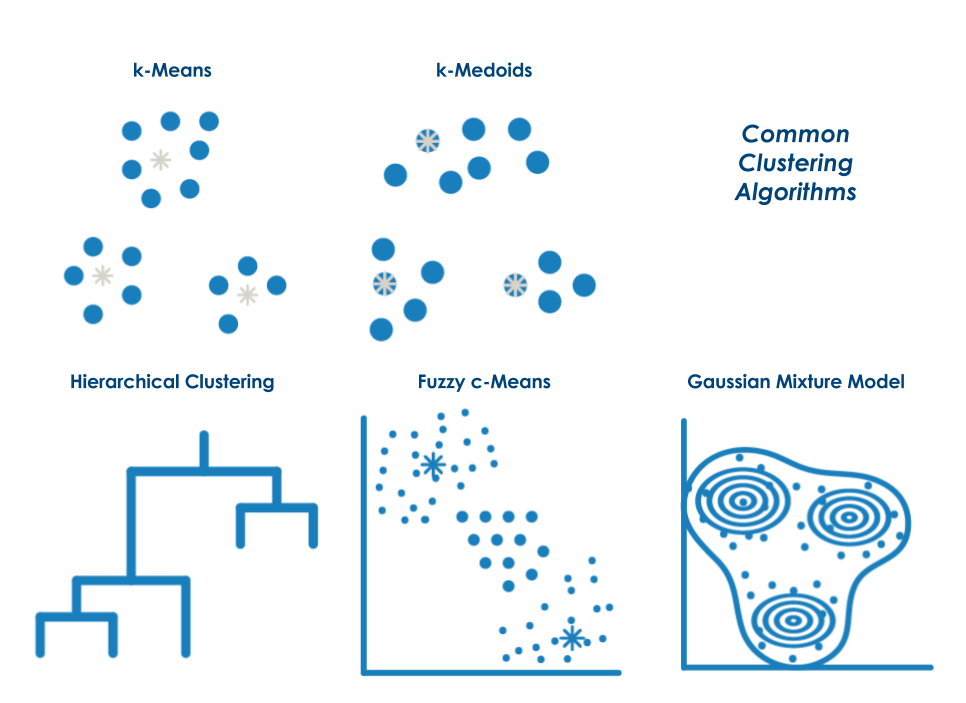
\includegraphics[width=0.8\linewidth]{imgs/unsupervisedtechniques}

\begin{quote}
La mayoría de las técnicas de aprendizaje no supervisado son una forma de análisis por cluster.
\end{quote}

En análisis por cluster, los datos son divididos en grupos de acuerdo con alguna métrica de similaridad o característica compartida. De esta forma los objetos o instancias en el mismo clúster son muy similares y los de distintos muy diferentes.

Los algoritmos de clustering se dividen en dos grandes grupos\footnote{Fuente: \url{https://es.mathworks.com/discovery/machine-learning.html}}:

\begin{itemize}
\item
  \textbf{Clustering rígido}, donde cada dato pertenece únicamente a un clúster.
\item
  \textbf{Clustering suave}, donde cada dato puede pertenecer a más de un clúster.
\end{itemize}

\textbf{k-means}

\begin{itemize}
\item
  \emph{¿Cómo trabaja?} Particiona datos en k número de clusters mutuamente excluyentes. El como de bien un punto se ajuste a un clúster determinado viene dado por su distancia al centro de dicho clúster.
\item
  \emph{¿Cuándo se usa?} Cuando el número de clusters es conocido y cuando se requiere un clustering rápido de grandes conjuntos de datos.
\item
  \emph{¿Cuál es el resultado?} Centroide de cada cluster.
\end{itemize}

\textbf{k-medoids}

\begin{itemize}
\item
  \emph{¿Cómo trabaja?} Algoritmo similar a k-medias pero requiere de que los centroides sean puntos u observaciones de la muestra.
\item
  \emph{¿Cuándo se usa?} Cuando el número de clusters es conocido. Para clustering rápido de datos categóricos. Para escalar a grandes conjuntos de datos.
\item
  \emph{¿Cuál es el resultado?} Observación o individuo de la muestra que actúa de centroide o medoide de cada cluster.
\end{itemize}

\textbf{Hierarchical Clustering}

\begin{itemize}
\item
  \emph{¿Cómo trabaja?} Produce conjuntos anidados de datos analizando similaridades entre pares de puntos y agrupando objetos en un arbol binario jerárquico.
\item
  \emph{¿Cuándo se usa?} Cuando se desconoce el número de clusters a los que darán lugar los datos. Cuando se requiere de visualización para guiar la elección.
\item
  \emph{¿Cuál es el resultado?} Dendograma mostrando la relación jerárquica entre los clusters.
\end{itemize}

\textbf{Self-Organizing Map}

\begin{itemize}
\item
  \emph{¿Cómo trabaja?} Red neuronal basada en clustering que transforma un conjunto de datos en un mapa 2D con preservación de topología.
\item
  \emph{¿Cuándo se usa?} Para observar datos de alta dimensionalidad en mapas 2D o 3D. Para deducir la dimensionalidad de los datos preservando su topología (forma).
\item
  \emph{¿Cuál es el resultado?} Representación en dimensión más baja (típicamente en 2D)
\end{itemize}

\textbf{Fuzzy c-Means}

\begin{itemize}
\item
  \emph{¿Cómo trabaja?} Agrupamiento difuso. Agrupamiento basado en particiones en el que los datos pueden estar en más de un cluster.
\item
  \emph{¿Cuándo se usa?} Cuando el número de clusters es conocido. Para reconocimento de patrones. Cuando los clusters se sobreponen o se solopan.
\item
  \emph{¿Cuál es el resultado?} Centro de los clústers (similar a k-means) pero con difusión (\emph{fuzziness}) de forma que las observaciones o individuos pueden pertenecer a más de 1 cluster.
\end{itemize}

\textbf{Gaussian Mixture Model}

\begin{itemize}
\item
  \emph{¿Cómo trabaja?} Modelo gaussiando mixto. Agrupación basada en particiones en la que los datos provienen de diferentes distribuciones normales multivariantes con ciertas probabilidades.
\item
  \emph{¿Cuándo se usa?} Cuando un punto puede pertenecer a más de un clúster. Cuando los clusters diferentes tamaños y correlaciones entre ellos.
\item
  \emph{¿Cuál es el resultado?} Modelo de distribuciones gausianas que proporciona la probabilidad de que una observación o individuo pertenezca a un clúster.
\end{itemize}

\hypertarget{tecnicas-de-clasificacion}{%
\section{Técnicas de Clasificación}\label{tecnicas-de-clasificacion}}

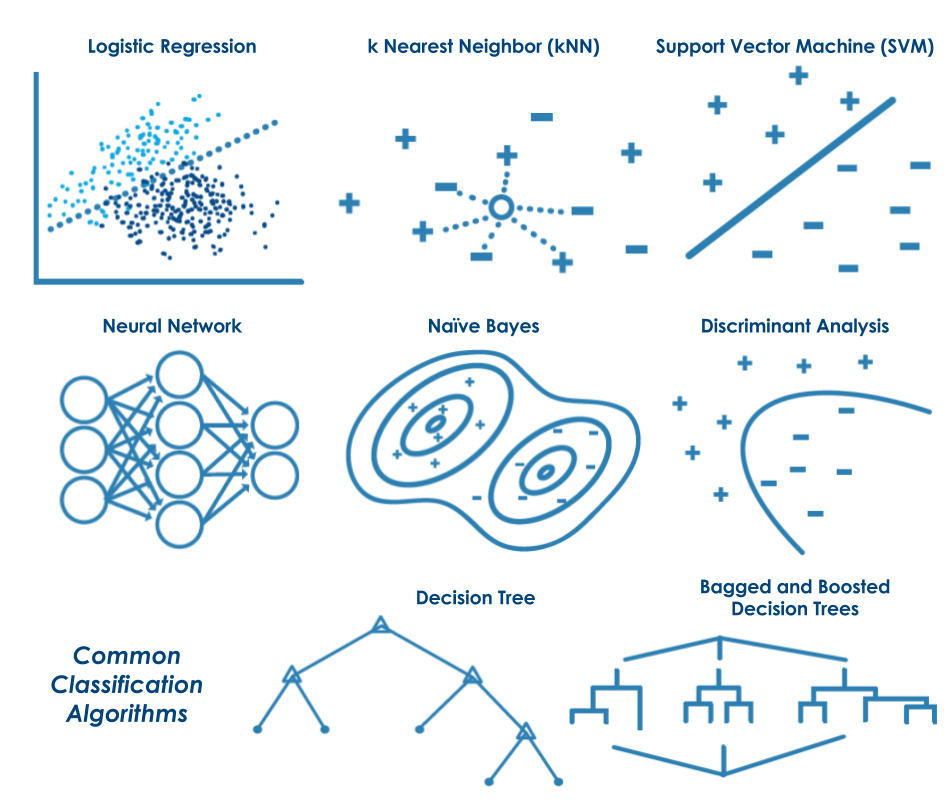
\includegraphics[width=0.8\linewidth]{imgs/classificationtechniques}

\textbf{Regresión Logística}

\begin{itemize}
\item
  \emph{¿Cómo trabaja?} Ajusta un modelo que puede predecir la probabilidad de que una respuesta binaria pertenezca a una clase u otra. Debido a su simplicidad, la regresión logística se utiliza comúnmente como punto de partida para los problemas de clasificación binaria.
\item
  \emph{¿Cuándo se usa?} Cuando los datos se pueden separar claramente por un solo límite lineal. Como una línea de base (\emph{baseline}) para evaluar más complejos métodos de clasificación.
\end{itemize}

\textbf{k Vecinos Cercanos (kNN)}

\begin{itemize}
\item
  \emph{¿Cómo trabaja?} kNN categoriza los objetos en función de las clases de su
  vecinos más cercanos en el conjunto de datos. Las predicciones de kNN suponen
  que los objetos cercanos entre sí son similares. Algunas de las métricas de distancia utilizadas para encontrar el vecino más cercano son: Euclides, \emph{bloque de la ciudad\_city block}, coseno y Chebychev.
\item
  \emph{¿Cuándo se usa?} Cuando se requiere un algoritmo simple para establecer
  reglas de aprendizaje de referencia o base. Cuando el uso de memoria del modelo entrenado no es una preocupación.
  Cuando la velocidad de predicción del modelo entrenado tampoco constituye una limitación.
\end{itemize}

\textbf{Support Vector Machines (SVM)}

\begin{itemize}
\item
  \emph{¿Cómo trabaja?} Clasifica datos encontrando el límite de decisión lineal (hiperplano) que separa todos los puntos de datos de una clase de los de la otra clase. El mejor hiperplano para una SVM es aquel con el mayor margen entre las dos clases, cuando los datos son linealmente separables. Si los datos no son linealmente separables, se utiliza una función de pérdida para penalizar los puntos en el lado equivocado del hiperplano Los SVM a veces usan una transformación de núcleo para transformar los datos no separables linealmente en dimensiones más altas donde un límite de decisión lineal puede ser encontrado.
\item
  \emph{¿Cuándo se usa?} Para datos que tienen exactamente dos clases.Para datos de alta dimensión, no linealmente separables.Cuando se necesita un clasificador que sea simple, fácil de interpretar y preciso.
\end{itemize}

\textbf{Redes Neuronales}

\begin{itemize}
\item
  \emph{¿Cómo trabaja?} Inspirada en el cerebro humano, una red neuronal consiste enredes de neuronas altamente conectadas que relacionan las entradas a las salidas deseadas La red se entrena de forma iterativa, modificando las fortalezas de las conexiones para que las entradas se asignen a la respuesta correcta.
\item
  \emph{¿Cuándo se usa?} Para modelar sistemas altamente no lineales. Cuando los datos están disponibles de forma incremental y se desea actualiza constantemente el modelo. Cuando podría haber cambios inesperados en su
  datos de entrada. Cuando la interpretabilidad del modelo no es una preocupación importante.
\end{itemize}

\textbf{Árboles de Decisión}

\begin{itemize}
\item
  \emph{¿Cómo trabaja?} Un árbol de decisión permite predecir respuestas a datos siguiendo
  las decisiones organizadas en un árbol, desde la raíz (inicio) hasta un nodo u hoja. Un árbol consiste en condiciones organizadas en forma de ramificaciones, donde el valor de un predictor se compara con un peso entrenado. Los número de ramas y los valores de los pesos se determinan
  en el proceso de entrenamiento. Algunas acciones adicionales, como la poda, se pueden usar para simplificar el modelo.
\item
  \emph{¿Cuándo se usa?} Cuando se necesita un algoritmo fácil de interpretar y
  rápido de ejecutar. Para minimizar el uso de memoria. Cuando la precisión predictiva alta no es un requisito.
\end{itemize}

\textbf{Bagging, Boosting}

\begin{itemize}
\item
  \emph{¿Cómo trabaja?} Varios árboles de decisión ``más débiles'' son
  combinados en un conjuto ``más fuerte''. Un árbol de decisión en bolsas (bagging) consta de árboles entrenados
  de forma independiente en los datos que se remuestrean (\emph{boostrapping}) a partir de los datos de entrada. \emph{Boosting} implica crear un modelo fuerte mediante la adición iterativa de modelos ``débiles'' y ajustando el peso de cada modelo débil para centrarse en ejemplos mal clasificados.
\item
  \emph{¿Cuándo se usa?} Cuando los predictores son categóricos (discretos) o se comportan
  no lineal.
\end{itemize}

\textbf{Análisis Discriminante}

\begin{itemize}
\item
  \emph{¿Cómo trabaja?} Clasifica los datos a partir de combinaciones lineales de los \emph{inputs}. El análisis discriminante asume que las diferentes clases de datos se pueden generar a partir de distribuciones gaussianas. Entrenar o ajustar un modelo de análisis discriminante implica encontrar los parámetros para la distribución gaussiana de cada clase.
\item
  \emph{¿Cuándo se usa?} Cuando necesitas un modelo simple que sea fácil de interpretar. Cuando el uso de la memoria durante el entrenamiento es una preocupación. Cuando necesitas un modelo que sea rápido para predecir.
\end{itemize}

\hypertarget{tecnicas-de-regresion}{%
\section{Técnicas de Regresión}\label{tecnicas-de-regresion}}

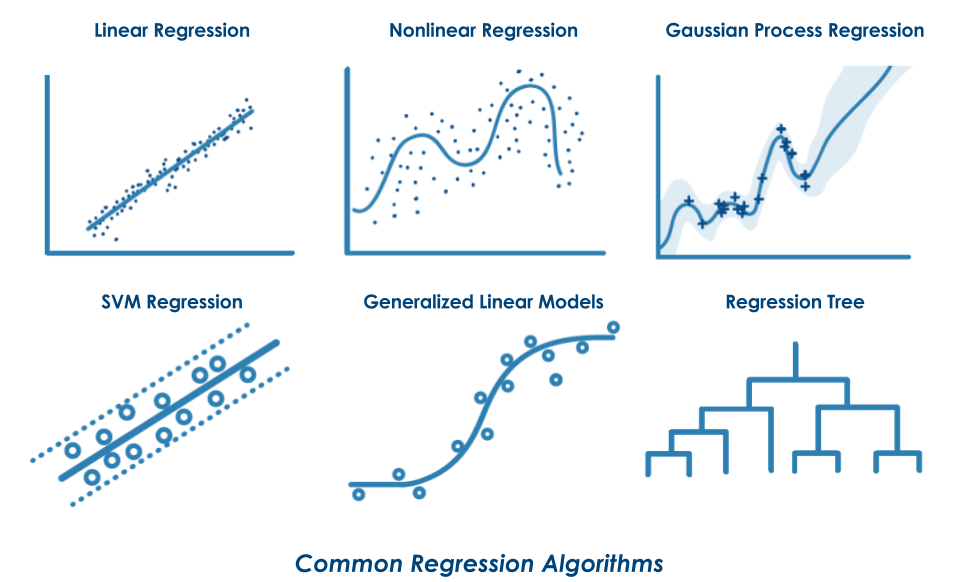
\includegraphics[width=0.8\linewidth]{imgs/regressiontechniques}

\textbf{Regresión Lineal}

\begin{itemize}
\item
  \emph{¿Cómo trabaja?} La regresión lineal es una clase de modelo estadístico utilizado para
  describir una variable de respuesta continua como una función lineal de una o más variables predictoras. Dado que los modelos de regresión lineal son simples de interpretar y fáciles de entrenar,
  a menudo constituyen el primer modelo que se ajusta a un nuevo conjunto de datos.
\item
  \emph{¿Cuándo se usa?} Cuando se necesita un algoritmo fácil de interpretar y rápido de ejecutar. Como línea de base para evaluar otros modelos de regresión más complejos.
\end{itemize}

\textbf{SVM Regression}

\begin{itemize}
\item
  \emph{¿Cómo trabaja?} Los algoritmos de regresión SVM funcionan como los algoritmos de clasificación SVM, pero están modificados para poder predecir una respuesta continua. En lugar de encontrar un hiperplano que
  separa los datos, los algoritmos de regresión SVM encuentran un modelo que se desvía (aleja) de los datos observados por un valor no mayor que una pequeña cantidad, con valores que son tan pequeños como
  posible (para minimizar la sensibilidad al error).
\item
  \emph{¿Cuándo se usa?} Para datos de alta dimensión (donde habrá una gran
  cantidad de variables predictoras)
\end{itemize}

\textbf{Generalized Linear Models}

\begin{itemize}
\item
  \emph{¿Cómo trabaja?} Un modelo lineal generalizado es un caso especial de modelo no lineal. Implica ajustar un combinación lineal de los \emph{inputs} a una función no lineal (la función de enlace) de los \emph{outputs}.
\item
  \emph{¿Cuándo se usa?} Cuando las variables de respuesta tienen un comportamiento de distribución no normal, como una variable de respuesta que se espera que sea siempre positiva.
\end{itemize}

\textbf{Regression Tree}

\begin{itemize}
\item
  \emph{¿Cómo trabaja?} Los árboles de decisión para la regresión son similares a los árboles de decisión para
  clasificación, pero se modifican para poder predecir respuestas continuas.
\item
  \emph{¿Cuándo se usa?} Cuando los predictores son categóricos (discretos) o se comportan
  no lineal.
\end{itemize}

\textbf{Gaussian Process Regression Model}

\begin{itemize}
\item
  \emph{¿Cómo trabaja?} Los modelos de regresión de procesos gaussianos (GPR) son modelos no paramétricos que se utilizan para predecir el valor de una variable de respuesta continua. Son ampliamente utilizados en
  el campo del análisis espacial para la interpolación en presencia de incertidumbre. GPR también se conoce como \emph{Kriging}.
\item
  \emph{¿Cuándo se usa?} Para la interpolación de datos espaciales.
\end{itemize}

\hypertarget{tecnicas-de-reduccion-de-dimension}{%
\section{Técnicas de Reducción de Dimensión}\label{tecnicas-de-reduccion-de-dimension}}

\textbf{Análisis de Componentes Principales (PCA)}

\begin{itemize}
\tightlist
\item
  \emph{¿Cómo trabaja?} Realiza una transformación lineal en los datos de forma que la mayor varianza o información en el conjunto de datos de alta dimensión es capturada por las primeras (pocas) componentes principales. La primera componente capturará la mayor varianza, seguida por la segunda componente principal, y así sucesivamente.
\end{itemize}

\textbf{Análisis Factorial}

\begin{itemize}
\tightlist
\item
  \emph{¿Cómo trabaja?} Identifia las correlaciones subyacentes entre las variables del conjunto de datos para proporcionar una representación en términos de un número pequeño de factores comunes latentes o no observables.
\end{itemize}

\hypertarget{otras-tecnicas}{%
\section{Otras `Técnicas'}\label{otras-tecnicas}}

\textbf{Minería de Textos}

\textbf{Video/Image Analytics}

\textbf{Speech Analytics}

\textbf{Stream Analytics}

\hypertarget{que-tecnica-utilizar}{%
\section{¿Qué técnica utilizar?}\label{que-tecnica-utilizar}}

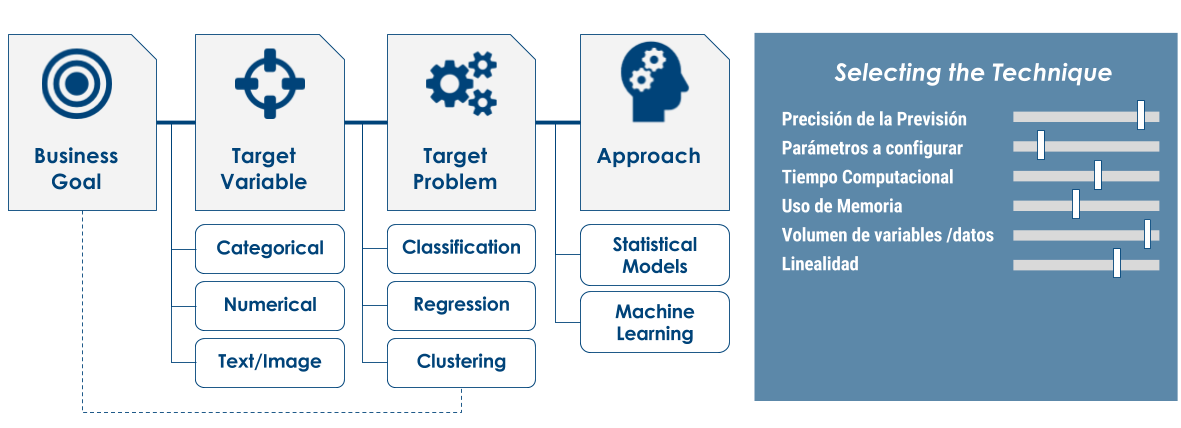
\includegraphics[width=0.9\linewidth]{imgs/choosealgorithm}

Elegir el algoritmo adecuado puede parecer abrumador---hay docenas de algoritmos de \emph{statistical learning}, y cada uno tiene una aproximación diferente. No existe un único mejor método o uno que sirva para todos los casos. Buscar el adecuado es a veces una tarea de prueba y error---incluso los científicos de datos con más experiencia no pueden saber si un algoritmo funcionará sin haberlo probado. La selección del algoritmo también depende del tamaño y del tipo de los datos con el que se está trabajando, los resultados que se quieren obtener y como dichos resultados serán usados.

El primer paso, y uno de los más importantes, es definir el objetivo del análisis que se va a realizar. Volviendo al esquema propuesto por Marr (\protect\hyperlink{ref-mar2015}{2017}) (presentado en \ref{modelizar}), \emph{Start with Strategy} implica que, antes de empezar con los datos, se empiece con la definición de los objetivos de negocio que se quieren alcanzar. Inmediatamente después se definen los datos y las métricas que estarán involucradas.

En este momento se conoce la naturaleza del problema y de la variable objetivo, por lo tanto se conoce si estamos delante de una variable continua o binaria, si se requiere de un modelo explicativo, si \emph{sólo} se requiere una segmentación, etc.

En consecuencia, una vez conocida la decisión que se requiere tomar y la variable objetivo que se analizará, se puede elegir el enfoque y modelo especíco que se va a utilizar.

Considera utilizar un \emph{modelo estadístico} si se debe priorizar el poder explicativo, se dispone de tiempo computacional y memoria para ajustar modelos relativamente complejos.

Algunas situaciones donde este enfoque es útil son:

\begin{itemize}
\tightlist
\item
  Proceso de concesión de créditos, con modelos supervisados por la entidad reguladora.
\item
  Asignación de presupuesto anual de marketing
\item
  Determinación de metas de venta por distribuidor, centro, etc.
\end{itemize}

Considera usar el \emph{machine learning} cuando se tenga una tarea compleja o un problema que involucre una gran cantidad de datos o variables, pero no exista fórmula o ecuación.

Por ejemplo, \emph{machine learning} es una buena opción si se requieren manejar situaciones como:

\begin{itemize}
\tightlist
\item
  Las reglas y ecuaciones de escritura a mano son muy complejas---como reconocimiento facial o de voz.
\item
  Las reglas de las tareas están cambiando constantemente---como en detección de fraude desde los registros de transacciones.
\item
  La naturaleza de los datos es cambiante y el programa necesita adaptarse---como en el trading automático, previsión de demanda de energía y predicción de tendencias en compras.
\end{itemize}

Algunas consideraciones al elegir un algoritmo son\footnote{Fuente: \url{https://docs.microsoft.com/es-es/azure/machine-learning/studio/algorithm-choice}}:

\begin{quote}
Precisión
\end{quote}

No siempre es necesario obtener la respuesta más precisa posible. A veces, una aproximación ya es útil, según para qué se la desee usar. Si es así, puede reducir el tiempo de procesamiento de forma considerable al usar métodos más aproximados. Otra ventaja de los métodos más aproximados es que tienden naturalmente a evitar el sobreajuste.

\begin{quote}
Tiempo (de entrenamiento)
\end{quote}

La cantidad de minutos u horas necesarios para modelizar varía mucho según el algoritmo. A menudo, el tiempo depende de la precisión (generalmente, uno determina al otro). Además, algunos algoritmos son más sensibles a la cantidad de datos que otros. Si el tiempo es limitado, esto puede determinar la elección del algoritmo, especialmente cuando el conjunto de datos es grande.

\begin{quote}
Cantidad de parámetros
\end{quote}

Los parámetros son los \emph{botones} que el analista activa al configurar un algoritmo. Son números que afectan al comportamiento del algoritmo, como la tolerancia a errores o la cantidad de iteraciones, o bien opciones de variantes de comportamiento del algoritmo. El tiempo de entrenamiento y la precisión del algoritmo a veces pueden ser muy sensibles y requerir solo la configuración correcta. Normalmente, los algoritmos con muchos parámetrosla mayor cantidad de pruebas para encontrar una buena combinación. La ventaja es que tener muchos parámetros normalmente indica que un algoritmo tiene mayor flexibilidad. Se puede lograr una precisión muy alta, siempre y cuando se encuentre la combinación correcta de configuraciones de parámetros.

\begin{quote}
Cantidad de variables
\end{quote}

Para ciertos tipos de datos, la cantidad de variables o características puede ser muy grande en comparación con la cantidad de datos. Este suele ser el caso de la genética o los datos textuales. Una gran cantidad de características puede trabar algunos algoritmos y provocar que el tiempo de procesamiento sea demasiado largo.

\begin{quote}
Linealidad
\end{quote}

Muchos algoritmos hacen uso de la linealidad. Los algoritmos de clasificación lineal suponen que las clases pueden estar separadas mediante una línea recta (o su análogo de mayores dimensiones). Entre ellos, se encuentran la regresión logística y las máquinas de vectores de soporte (svm). Los algoritmos de regresión lineal suponen que las tendencias de datos siguen una línea recta. Estas suposiciones no son incorrectas para algunos problemas, pero en otros disminuyen la precisión.

\begin{quote}
Casos especiales
\end{quote}

Algunos algoritmos hacen determinadas suposiciones sobre la estructura de los datos o los resultados deseados. Si encuentra uno que se ajuste a sus necesidades, este puede ofrecerle resultados más útiles, predicciones más precisas o tiempos de procesamiento más cortos.

\hypertarget{evaluacion-de-modelos}{%
\chapter{Evaluación de modelos}\label{evaluacion-de-modelos}}

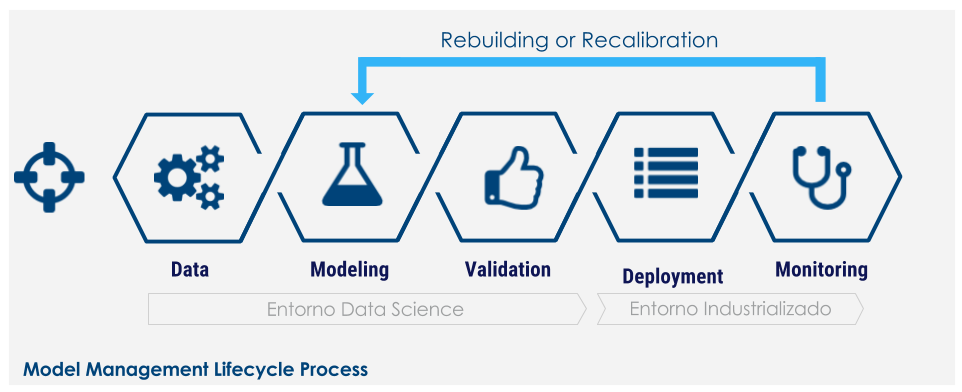
\includegraphics[width=0.9\linewidth]{C:/Users/romy.rodriguez/Documents/INNOVA/Formacion/MiCurso/ModelizacionR/imgs/modellingcycle}

El ciclo de vida de un modelo empieza con su propia definición, pasando por la extracción y tratamiento de los datos y la evaluación, tanto antes de ponerlo en producción, como en la monitorización de su calidad predictiva.

La diagnosis o evaluación es la clave para lograr un ecosistema de modelos que impacte en la organización. Hay muchas métricas para evaluar como de bien o de mal funciona un modelo o algoritmo. Para determinar cuáles usar en un problema particular, necesitamos formas sistemáticas de evaluar cómo funcionan los diferentes métodos y comparar uno con otro. La evaluación no es tan simple como podría parecer a primera vista.

La diagnosis de los modelos puede realizarse desde dos perspectivas:

\begin{itemize}
\tightlist
\item
  \textbf{Negocio} y
\item
  \textbf{Estadística}.
\end{itemize}

Ambas pueden ser utilizadas para monitorizar la calidad de los modelos en producción. La frecuencia de análisis depende del tipo de modelo.

\begin{itemize}
\item
  \textbf{Diagnosis de Negocio}: Se refiere a la utilización de métricas que indican si se cumplen las hipótesis sobre las cuales se ha construido el modelo, además de evaluar su calidad predictiva. Ejemplo de estas métricas son: R2, MAPE, AUC, LIFT, etc
\item
  \textbf{Diagnosis Estadística}: Se refiere a la discusión del significado de los resultados, teniendo en cuenta el sentido del negocio. Elementos susceptibles de esta interpretación son: parámetros, análisis decom, due-to, etc.
\end{itemize}

\hypertarget{diagnosis-de-negocio}{%
\section{Diagnosis de Negocio}\label{diagnosis-de-negocio}}

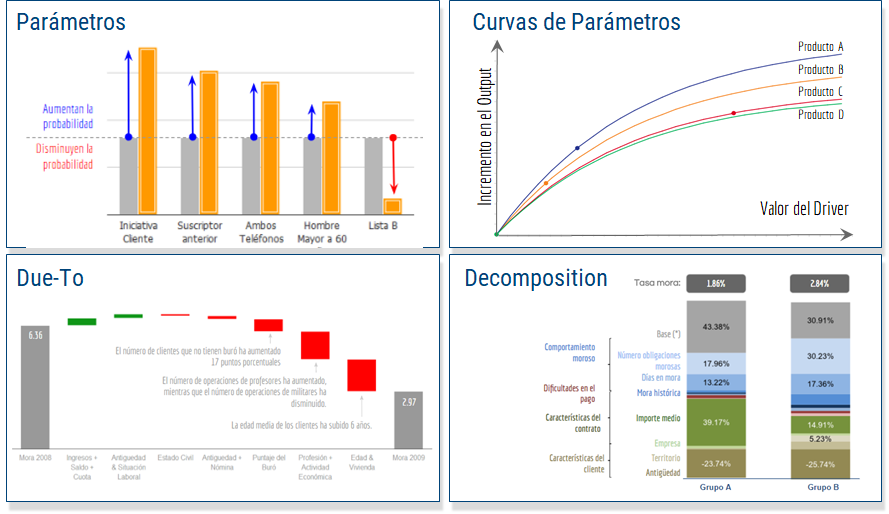
\includegraphics[width=0.9\linewidth]{C:/Users/romy.rodriguez/Documents/INNOVA/Formacion/MiCurso/ModelizacionR/imgs/evaluanegocio}

\begin{itemize}
\item
  Los \textbf{parámetros} de los modelos estadisticos sirven para cuantificar el efecto de las palancas. Su interpretación depende de la propia especificación del modelo. Los principales tipos de parámetros son: elasticidad, semi-elasticidad, \emph{piecewise}, \emph{yes/no}. Si el output es 0-1, la interpretación de los parámetros depende de la función enlace utilizada (\emph{logit} o \emph{probit}).
\item
  Análisis de \textbf{Descomposición}. Mide el efecto de cada \emph{input} o \emph{driver} sobre el \emph{output} de un periodo
\item
  Análisis de \textbf{due-to}. Compara el efecto de los \emph{inputs} o \emph{drivers} en el \emph{output} entre dos periodos
\end{itemize}

\hypertarget{evaluacion-en-respuesta-binaria}{%
\section{Evaluación en Respuesta Binaria}\label{evaluacion-en-respuesta-binaria}}

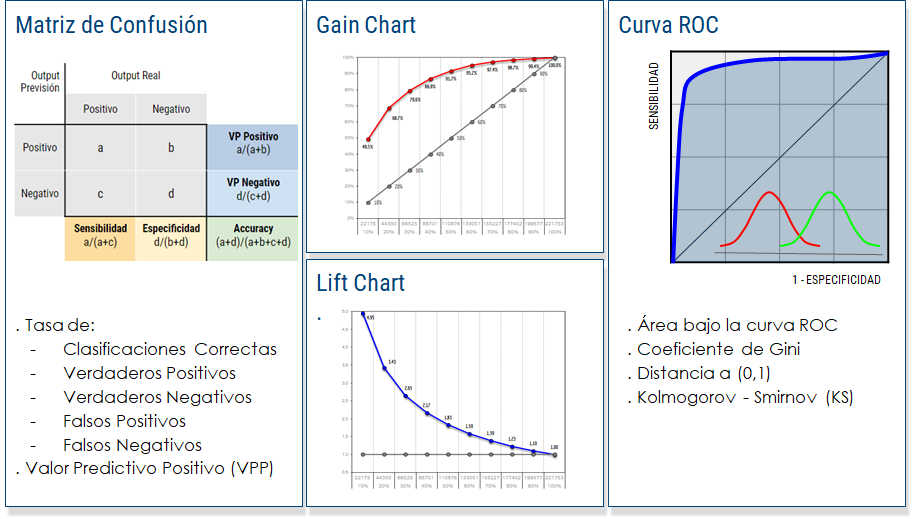
\includegraphics[width=0.9\linewidth]{C:/Users/romy.rodriguez/Documents/INNOVA/Formacion/MiCurso/ModelizacionR/imgs/evaluabinario}

No todos los problemas son iguales, con lo que no todos los problemas pueden usar las mismas métricas de evaluación. En esta sección veremos las métricas más usuales para los tipos de problemas que nos podemos encontrar. Si nos centramos en modelos supervisados, nos encontramos básicamente dos problemas distintos: clasificación y regresión.

\hypertarget{clasificacion}{%
\subsection{Clasificación}\label{clasificacion}}

En los problemas de clasificación tenemos la variable objetivo que son las clases o etiquetas que debemos predecir y una serie de variables que son los predictores. Es decir, usando los predictores obtenemos una etiqueta. Nos podemos encontrar con problemas de clasificación binaria (dos clases) o múltiple (más de dos clases).

Para simplificar nos centraremos en la clasificación binaria, pero lo podemos trasladar a los problemas de clasificación múltiple.

\hypertarget{confusion-matrix}{%
\subsubsection{Confusion matrix}\label{confusion-matrix}}

La confusion matrix o matriz de confusión muestra el número de predicciones correctas e incorrectas hechas por el modelo de clasificación en comparación con los resultados reales en los datos. La matriz de confusión es una matriz \(n \times n\), dónde \(n\) es el número de clases. La siguiente tabla muestra una matriz de confusión de \(2x2\) para dos clases (positiva y negativa).

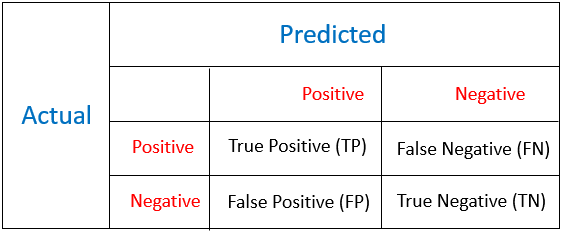
\includegraphics[width=0.8\linewidth]{C:/Users/romy.rodriguez/Documents/INNOVA/Formacion/MiCurso/ModelizacionR/imgs/confusionmatrix}

\begin{itemize}
\tightlist
\item
  \textbf{Accuracy}: la proporción del número total de predicciones correctas.
\end{itemize}

\[ACC = \frac{TP+TN}{TP+TN+FP+FN}\]

\begin{itemize}
\tightlist
\item
  \textbf{Positive Predictive Value or Precision}: la proporción de casos positivos que fueron identificados correctamente.
\end{itemize}

\[PPV = \frac{TP}{TP+FP}\]

\begin{itemize}
\tightlist
\item
  \textbf{Negative Predictive Value}: la proporción de casos negativos que fueron identificados correctamente.
\end{itemize}

\[ 
NPV = \frac{TN}{TN+FN}
\]

\begin{itemize}
\tightlist
\item
  \textbf{Sensitivity or Recall}: la proporción de casos positivos reales que están correctamente identificados.
\end{itemize}

\[TPR = \frac{TP}{TP+FN}\]

\begin{itemize}
\tightlist
\item
  \textbf{Specificity}: la proporción de casos negativos reales que están correctamente identificados.
\end{itemize}

\[TNR = \frac{TN}{TN+FP}\]

\hypertarget{log-loss}{%
\subsubsection{Log-Loss}\label{log-loss}}

La log-loss o pérdida logarítmica entra en los detalles más finos de un clasificador. En particular, si la salida bruta del clasificador es una probabilidad numérica en lugar de una etiqueta de clase de \(0\) o \(1\), se puede usar la log-loss. La probabilidad se puede entender como un indicador de confianza. Si la etiqueta es \(0\) pero el clasificador cree que pertenece a la clase \(1\) con probabilidad de \(0,51\). Aunque el clasificador estaría cometiendo un error de clasificación, el error se comente por poco, ya que la probabilidad está muy cerca del punto de corte de \(0.5\). La log-loss es una medición de precisión que incorpora esta idea de confianza probabilística.

La log-loss para un clasificador binario es

\[LogLoss = - \frac{1}{n} \sum_{i=1}^{n} y_i \log p_i + (1-y_i) \log (1-p_i)\]

donde \(n\) es el número de registros, \(y_i\) es la etiqueta de la muestra \(i\), y \(p_i\) es la probabilidad del obtenida en el modelo.

\hypertarget{curvas-roc}{%
\subsubsection{Curvas ROC}\label{curvas-roc}}

Para los modelos de clasificación obtenidos a partir de una probabilidad se suelen usar las curvas ROC. Una curva ROC (acrónimo de Receiver Operating Characteristic, o Característica Operativa del Receptor) es una representación gráfica de la sensitivity (TPR) frente a la specificity (TNR) para un sistema clasificador binario según se varía el umbral de discriminación.

La curva ROC se puede usar para generar estadísticos que resumen el rendimiento (o la efectividad, en su más amplio sentido) del clasificador. A continuación se proporcionan algunos:

\begin{itemize}
\tightlist
\item
  El punto de inserción de la curva ROC con la línea convexa a la línea de discriminación.
\item
  El área entre la curva ROC y la línea de convexo-paralela discriminación.
\item
  El área bajo la curva ROC, llamada comúnmente AUC (area under curve).
\end{itemize}

El indicador más utilizado en muchos contextos es el área bajo la curva ROC o AUC. Este índice se puede interpretar como la probabilidad de que un clasificador ordenará o puntuará una instancia positiva elegida aleatoriamente más alta que una negativa.

En la figura abajo se muestran tres ejemplos de curvas ROC. La gráfica de la izquierda es la curva de un modelo perfecto, la del medio es la de un caso real con una \(AUC = 0.8\) y la de la derecha es la gráfico de un modelo no informativo.

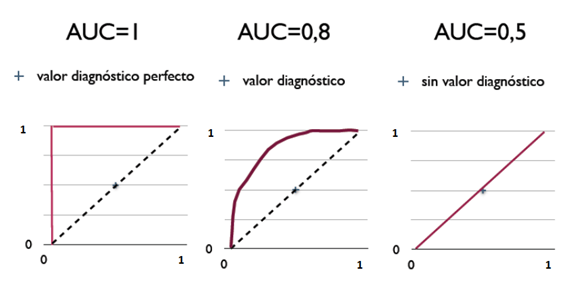
\includegraphics[width=0.8\linewidth]{C:/Users/romy.rodriguez/Documents/INNOVA/Formacion/MiCurso/ModelizacionR/imgs/curvasroc}

\hypertarget{graficos-de-ganancia-y-elevacion-gain-and-lift-charts}{%
\subsubsection{Gráficos de ganancia y elevación (Gain and Lift Charts)}\label{graficos-de-ganancia-y-elevacion-gain-and-lift-charts}}

La ganancia o la elevación es una medida de la efectividad de un modelo de clasificación calculado como la relación entre los resultados obtenidos con y sin el modelo. Los gráficos de ganancia y elevación son ayudas visuales para evaluar el rendimiento de los modelos de clasificación. Sin embargo, en contraste con la matriz de confusión que evalúa los modelos en toda la población, los gráficos de ganancia o elevación evalúan el modelo en una porción de la población.

Para crear estos gráficos es necesario crear un ranking basado en la creabilidad de la predicción hecha por el modelo.

En la figura tenemos un ejemplo de como obtener los puntos de las curvas de ganancia y elevación, y sus correspondientes gráficos.

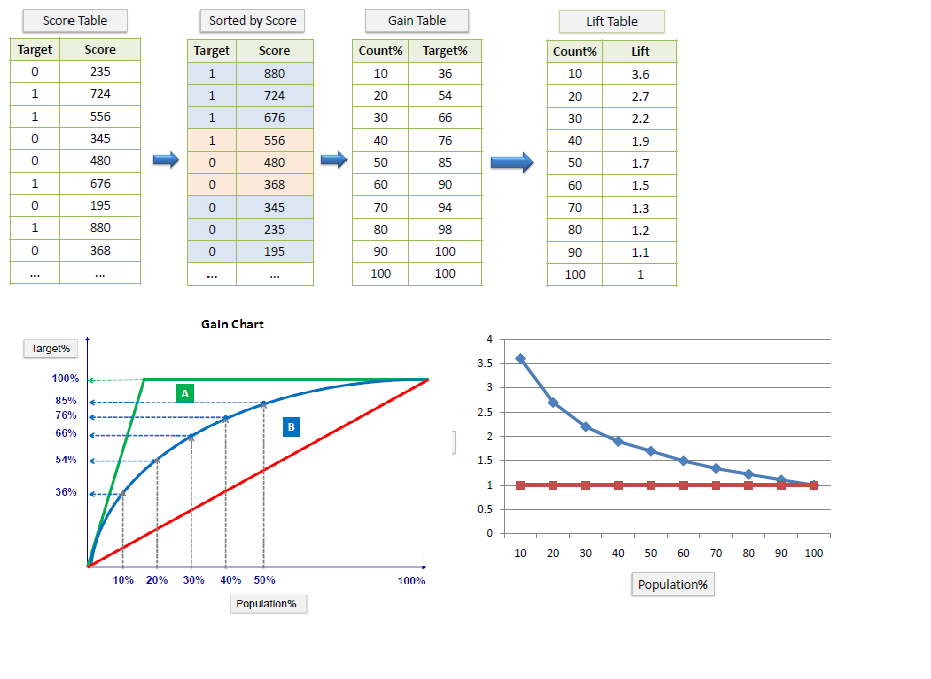
\includegraphics[width=0.8\linewidth]{C:/Users/romy.rodriguez/Documents/INNOVA/Formacion/MiCurso/ModelizacionR/imgs/gainlift}

Igual que las curvas ROC, se busca el mayor AUC en las curvas de ganancia. Mientras que para los gráficos de elevación el modelo perfecto es el que la diferencia entre la línea azul y roja es nula. En otras palabras queremos una AUC mínima del gráfico de elevación.

\hypertarget{medidas-de-desigualdad}{%
\subsection{Medidas de desigualdad}\label{medidas-de-desigualdad}}

\hypertarget{el-coeficiente-de-gini}{%
\subsubsection{El coeficiente de Gini}\label{el-coeficiente-de-gini}}

El coeficiente de Gini es una medida de la desigualdad ideada por el estadístico italiano Corrado Gini. El coeficiente de Gini es un número entre \(0\) y \(1\), en donde \(0\) se corresponde con la perfecta igualdad y donde el valor \(1\) se corresponde con la perfecta desigualdad.

El coeficiente de Gini se calcula como una proporción de las áreas en el diagrama de la curva de Lorenz. De forma resumida, la Curva de Lorenz es una gráfica de concentración acumulada de la distribución superpuesta a la curva de la distribución de frecuencias de los individuos, y su expresión en porcentajes es el índice de Gini. El coeficiente de Gini puede obtener mediante la siguiente fórmula:

\[G = \left| 1-\sum_{k=1}^{n-1} (X_{k+1}-X_k)(Y_{k+1}+Y_k) \right|\]

donde \(X\) es la proporción acumulada de la variable población, \(Y\) es la proporción acumulada de la variable a estudiar la desigualdad y \(n\) es el número de la población.

\hypertarget{indice-de-entropia}{%
\subsubsection{Índice de entropía}\label{indice-de-entropia}}

El índice de entropía generalizado se ha propuesto como una medida de la desigualdad en una población. Se deriva de la teoría de la información como una medida de redundancia en los datos. En la teoría de la información, una medida de redundancia puede interpretarse como no aleatoriedad o compresión de datos; por lo tanto, esta interpretación también se aplica a este índice.

La fórmula de la entropía general para un valor real \(\alpha\) es:

\[GE(\alpha) = \begin{cases}
       \frac{1}{n\alpha (\alpha -1)} \sum_{i=1}^{n} \left(\left( \frac{y_i}{\bar{y}} \right) ^{\alpha} -1\right), &\quad \alpha\neq0,1 ,\\
       \frac{1}{n} \sum_{i=1}^{n} \frac{y_i}{\bar{y}} \ln \frac{y_i}{\bar{y}} &\quad \alpha = 1 ,\\
       -\frac{1}{n} \sum_{i=1}^{n} \ln \frac{y_i}{\bar{y}} &\quad \alpha = 0 .\\
     \end{cases}\]

donde \(n\) el número de muestras y \(y\) es la medida de desigualdad.

\hypertarget{evaluacion-en-respuesta-continua}{%
\section{Evaluación en Respuesta Continúa}\label{evaluacion-en-respuesta-continua}}

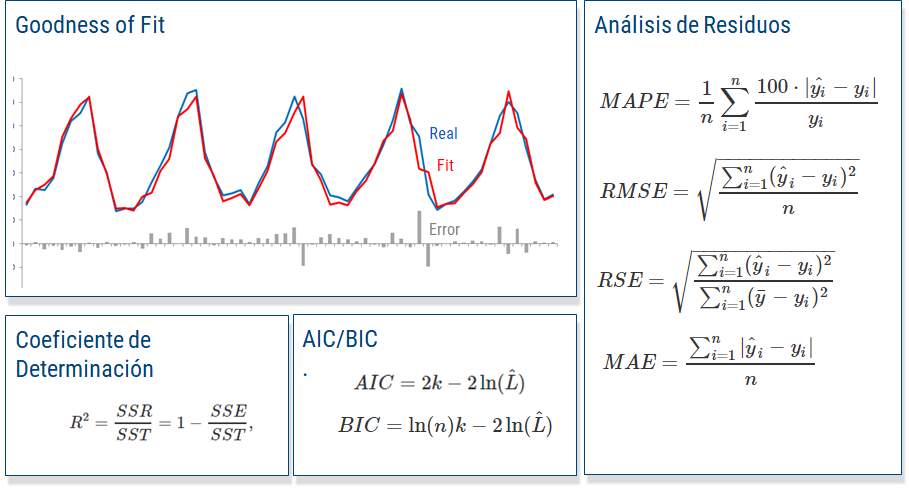
\includegraphics[width=0.9\linewidth]{C:/Users/romy.rodriguez/Documents/INNOVA/Formacion/MiCurso/ModelizacionR/imgs/evaluacontinuo}

\hypertarget{modelos-de-regresion}{%
\subsection{Modelos de Regresión}\label{modelos-de-regresion}}

En los problemas de regresión siempre tenemos una variable numérica dependiente que es la que queremos predecir y el resto son los predictores. Para evaluar los modelos de regresión tenemos varias métricas para evaluar el error cometido en al predicción:

\begin{itemize}
\tightlist
\item
  \textbf{RMSE} (root mean squared error) o error cuadrado medio: RMSE es la métrica más popular para medir la tasa de error de un modelo de regresión.
\end{itemize}

\[RMSE = \sqrt {\frac{\sum_{i=1}^{n} (\hat{y}_i - y_i)^2}{n}}\]

donde \(n\) es el número de muestras, \(\hat{y}_i\) el valor predicho de la variable objetivo y \(y_i\) el valor real de la variable objetivo.

\begin{itemize}
\tightlist
\item
  \textbf{MAE} (mean abosulte error) o error absoluto medio:
\end{itemize}

\[MAE = \frac{\sum_{i=1}^{n} | \hat{y}_i - y_i |}{n}\]

donde \(n\) es el número de muestras, \(\hat{y}_i\) el valor predicho de la variable objetivo y \(y_i\) el valor real de la variable objetivo.

\begin{itemize}
\tightlist
\item
  \textbf{RSE} (relative squared error) o error relativo cuadrado:
\end{itemize}

\[RSE = \sqrt \frac{\sum_{i=1}^{n} (\hat{y}_i - y_i)^2}{\sum_{i=1}^{n} (\bar{y} - y_i)^2}\]

donde \(n\) es el número de muestras, \(\bar{y}\) es la media de la variable objetivo, \(\hat{y}_i\) el valor predicho de la variable objetivo y \(y_i\) el valor real de la variable objetivo.

\begin{itemize}
\tightlist
\item
  \textbf{RAE} (relative absolute error) o error relativo absoluto:
\end{itemize}

\[RAE = \frac{\sum_{i=1}^{n} |\hat{y}_i - y_i|}{\sum_{i=1}^{n} |\bar{y} - y_i|}\]

donde \(n\) es el número de muestras, \(\bar{y}\) es la media de la variable objetivo, \(\hat{y}_i\) el valor predicho de la variable objetivo y \(y_i\) el valor real de la variable objetivo.

\begin{itemize}
\tightlist
\item
  \textbf{Coeficiente \(R^2\)}: \(R^2\) resume el poder explicativo del modelo de regresión y se calcula a partir de los términos de las sumas de cuadrados. El coeficiente \(R^2\) toma valores entre \(0\) y \(1\), si \(R^2=1\) la regresión es perfecta.
\end{itemize}

\[R^2 = \frac {SSR}{SST} = 1 - \frac{SSE}{SST}, \]

donde \[SST = \sum_{i=1}^{n} (y - \bar{y})^2 ,\]

\[SSR = \sum_{i=1}^{n} (\hat{y} - \bar{\hat{y}})^2 ,\]

\[SSE = \sum_{i=1}^{n} (y-\hat{y})^2 .\]

\hypertarget{modelos-de-series-temporales}{%
\subsection{Modelos de Series temporales}\label{modelos-de-series-temporales}}

Las series temporales son básicamente un problema de regresión. La diferencia es que hay una variable temporal y el objetivo es predecir el futuro dado un histórico. Por lo tanto, las métricas utilizadas son las mismas que las usadas para los problemas de regresión vistas en la sección anterior.

Otras métricas usadas frecuentemente para la evaluación de series temporales son:

\textbf{MAPE}

\emph{MAPE} viene de \emph{Mean Absolute Percentage Error}. Los errores porcentuales tienen la ventaja de ser independientes de la escala y, por lo tanto, se utilizan con frecuencia para comparar el rendimiento del pronóstico entre diferentes conjuntos de datos. MAPE es el más usual.

\[MAPE = \frac{1}{n} \sum_{i=1}^{n} \frac{100·|\hat{y_i}-y_i|}{y_i}\]

\textbf{AIC}

\emph{AIC} viene de \emph{Akaike information criterion}. Se define como

\[AIC = 2k-2\ln (\hat{L})\]

Dado un conjunto de modelos candidatos para los datos, el modelo preferido es el que tiene el valor mínimo en el AIC. Por lo tanto AIC no sólo recompensa la bondad de ajuste, sino también incluye una penalidad, que es una función creciente del número de parámetros estimados.

\textbf{BIC}

\emph{BIC}**\_ viene de \emph{Bayesian Information Criterion})\_. Se define como

\[BIC = \ln (n) k - 2 \ln (\hat{L})\]

donde \(\hat{L}\) es máximo de la función de verosimilitud, \(n\) es el número de muestras, \(k\) es el número de parámetros estimados por el modelo.

La fórmula del BIC es similar a la fórmula del AIC, pero con una penalización distinta que varia según el número de muestras de los datos.

\hypertarget{evaluacion-en-clustering}{%
\section{\texorpdfstring{Evaluación en \emph{Clustering}}{Evaluación en Clustering}}\label{evaluacion-en-clustering}}

El \emph{Clustering} es una forma de tratar los datos para los que no se conocen o no están definidos los grupos. Por tanto, tenemos que \textbf{conceptualizar} los grupos. Este hecho dificultad evaluar la calidad de los clasificación obtenida.

\hypertarget{silueta}{%
\subsection{Silueta}\label{silueta}}

El coeficiente silueta proporciona una representación gráfica del grado de integración de un objeto en su cluster. El coeficiente silueta de un objeto \(i\) se define como:

\[s_i=\dfrac{b_i -a_i}{max(b_i -a_i)}\]

donde \(a_i\) denota la distancia media entre el objeto \(i\) y todos los otros objetos de su cluster y \(b_i\) denota la distancia media mínima entre \(i\) y los objetos de otros clusters.
Los objetos con un coeficiente de silueta \(s_i\) alto están bien integrados en su cluster; aquéllos con un si bajo tienden a estar entre clusters.

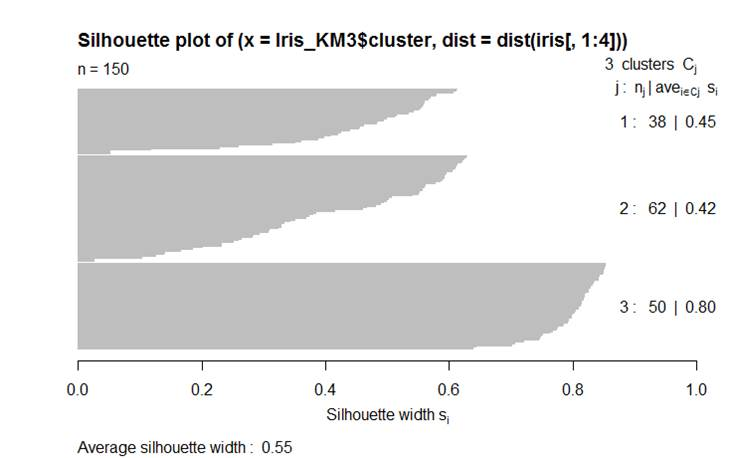
\includegraphics[width=0.9\linewidth]{C:/Users/romy.rodriguez/Documents/INNOVA/Formacion/MiCurso/ModelizacionR/imgs/silueta}

\hypertarget{metodos-de-re-muestreo}{%
\section{Métodos de re-muestreo}\label{metodos-de-re-muestreo}}

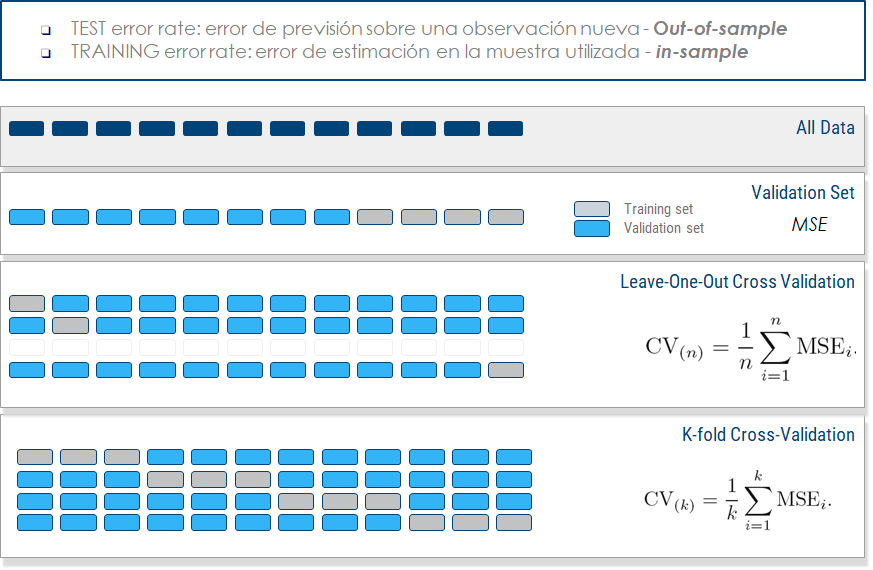
\includegraphics[width=0.8\linewidth]{C:/Users/romy.rodriguez/Documents/INNOVA/Formacion/MiCurso/ModelizacionR/imgs/traintess}

\hypertarget{training-testing}{%
\subsection{Training \& testing}\label{training-testing}}

Lo primero que debemos hacer para conseguir una buena evaluación es dividir los datos en dos subconjuntos. Uno para entrenar el modelo (training) y otro para evaluar el modelo (testing). El partición entre estos dos subconjuntos suele hacerse de forma aleatoria, aunque según el problema podemos usar otros criterios. Por ejemplo, si los datos que tenemos son una serie temporal, entonces podemos dividirlos a partir de un cierto tiempo. Es decir, coger como test los datos más recientes.

La razón de hacer esta división es usar los datos del subconjunto training para entrenar el modelo y luego evaluar los datos del testing. De esta manera simulamos correctamente una evaluación, ya que no podemos evaluar unos datos si hemos entrenado con ellos. Por lo tanto, los datos de testing no deben ser observados por el algoritmo.

\hypertarget{cross-validation}{%
\subsection{Cross validation}\label{cross-validation}}

El procedimiento que se suele usar para evaluar un modelo es cross validation o validación cruzada. La idea básica de cross validation consiste en dividir los datos en \(k\) subconjuntos. Cada subconjunto se predice mediante un modelo entrenado con el resto. De esta manera podemos hacer una evaluación sobre todos los datos y evitamos el problema de obtener una muestra sesgada si sólo lo hiciéramos una vez.

\hypertarget{practica-en-r}{%
\section{Práctica en R}\label{practica-en-r}}

Evaluaremos la calidad predictiva de dos modelos:

\begin{itemize}
\tightlist
\item
  Cuando la variable respuesta es binaria.
\item
  Cuando la variable respuesta es contínua.
\end{itemize}

\hypertarget{preparacion-de-los-datos}{%
\subsection{Preparación de los datos}\label{preparacion-de-los-datos}}

\begin{quote}
Definimos el Entorno de Trabajo
\end{quote}

El primer paso es crear una carpeta con nuestros modelos y resultados dentro de nuestro espacio de trabajo (proyecto).

\begin{itemize}
\tightlist
\item
  Obtenemos la ruta completa del directorio de trabajo\footnote{Si queremos cambiar la ruta, podemos hacer `myWd \textless{}- setwd(``Ruta y Nombre de la carpeta'')'.}.
\end{itemize}

\begin{Shaded}
\begin{Highlighting}[]
\NormalTok{myWD <-}\StringTok{ }\KeywordTok{getwd}\NormalTok{() }
\end{Highlighting}
\end{Shaded}

\begin{itemize}
\tightlist
\item
  Elegimos un nombre para nuestra carpeta con resultados
\end{itemize}

\begin{Shaded}
\begin{Highlighting}[]
\NormalTok{myWorkingFolderName <-}\StringTok{ 'ModelResults'} 
\end{Highlighting}
\end{Shaded}

\begin{itemize}
\tightlist
\item
  Creamos la carpeta donde guardaremos nuestros resultados y ficheros
\end{itemize}

\begin{Shaded}
\begin{Highlighting}[]
\KeywordTok{dir.create}\NormalTok{( }\KeywordTok{paste0}\NormalTok{(}\KeywordTok{getwd}\NormalTok{(),}\StringTok{"/"}\NormalTok{,myWorkingFolderName))}
\end{Highlighting}
\end{Shaded}

\begin{quote}
Accedemos a los datos originales
\end{quote}

\begin{itemize}
\tightlist
\item
  Cargamos la librería \texttt{insuranceData} que contiene los datos que utilizaremos\footnote{\url{https://CRAN.R-project.org/package=insuranceData}}
\end{itemize}

\begin{Shaded}
\begin{Highlighting}[]
\ControlFlowTok{if}\NormalTok{ (}\OperatorTok{!}\KeywordTok{require}\NormalTok{(insuranceData)) }\KeywordTok{install.packages}\NormalTok{(}\StringTok{'insuranceData'}\NormalTok{)}
\KeywordTok{library}\NormalTok{(insuranceData)}
\end{Highlighting}
\end{Shaded}

\begin{itemize}
\tightlist
\item
  Para ver los contenidos de la librería \texttt{insuranceData} ejecutamos:
\end{itemize}

\begin{Shaded}
\begin{Highlighting}[]
\KeywordTok{data}\NormalTok{(}\DataTypeTok{package=}\StringTok{'insuranceData'}\NormalTok{)}
\end{Highlighting}
\end{Shaded}

\begin{itemize}
\item
  Vemos que hay 10 datasets. Trabajaremos con el primero: \texttt{AutoBi} (\emph{Automobile Bodily Injury Claims}\footnote{\url{https://www.rdocumentation.org/packages/insuranceData/versions/1.0/topics/AutoBi}}).
\item
  Cargamos el conjunto de datos seleccionado: \textbf{pérdidas en accidentes de coches}
\end{itemize}

\begin{Shaded}
\begin{Highlighting}[]
\KeywordTok{data}\NormalTok{(}\StringTok{"AutoBi"}\NormalTok{)}
\end{Highlighting}
\end{Shaded}

\begin{itemize}
\item
  Descripción de las 8 variables del conjunto de datos (\emph{tabla}) `AutoBi':

  \begin{enumerate}
  \def\labelenumi{\arabic{enumi}.}
  \tightlist
  \item
    \texttt{Casenum}. Identificador de la reclamación (esta variable no se utiliza en los modelos)
  \item
    \texttt{Attorney}. Indica si el reclamante está representado por un \textbf{abogado} (1= Sí, 2 = No)
  \item
    \texttt{Clmsex}. \textbf{Sexo} del reclamante (1 = Hombre, 2 = Mujer)
  \item
    \texttt{Marital}. \textbf{Estado Civil} del reclamante (1 = Casado, 2 = Soltero, 3 = Viudo, 4 = divorciado/separado)
  \item
    \texttt{Clminsur}. Indica si el conductor del vehículo del reclamante estaba o no \textbf{asegurado} (1 = Si, 2 = No, 3 = No aplica)
  \item
    \texttt{Seatbelt}. Si el reclamante llevaba o no un \textbf{cinturón} de seguridad en el asiento infantil (1 = Si, 2 = No, 3 = No Aplica)
  \item
    \texttt{Clmage}. \textbf{Edad} del reclamante.
  \item
    \texttt{Loss\ (*)}. La \textbf{pérdida económica} total del reclamante (en miles). Esta es la variable objetivo o dependiente del conjunto de datos.
  \end{enumerate}
\item
  Revisamos el contenido de la tabla y el tipo de datos que contiene
\end{itemize}

\begin{Shaded}
\begin{Highlighting}[]
\KeywordTok{str}\NormalTok{(AutoBi)}
\end{Highlighting}
\end{Shaded}

\begin{verbatim}
FALSE 'data.frame': 1340 obs. of  8 variables:
FALSE  $ CASENUM : int  5 13 66 71 96 97 120 136 152 155 ...
FALSE  $ ATTORNEY: int  1 2 2 1 2 1 1 1 2 2 ...
FALSE  $ CLMSEX  : int  1 2 1 1 1 2 1 2 2 1 ...
FALSE  $ MARITAL : int  NA 2 2 1 4 1 2 2 2 2 ...
FALSE  $ CLMINSUR: int  2 1 2 2 2 2 2 2 2 2 ...
FALSE  $ SEATBELT: int  1 1 1 2 1 1 1 1 1 1 ...
FALSE  $ CLMAGE  : int  50 28 5 32 30 35 19 34 61 NA ...
FALSE  $ LOSS    : num  34.94 10.892 0.33 11.037 0.138 ...
\end{verbatim}

\begin{itemize}
\tightlist
\item
  Exploramos el contenido con estadísticos descriptivos básicos
\end{itemize}

\begin{Shaded}
\begin{Highlighting}[]
\KeywordTok{summary}\NormalTok{(AutoBi)}
\end{Highlighting}
\end{Shaded}

\begin{verbatim}
FALSE     CASENUM         ATTORNEY         CLMSEX         MARITAL     
FALSE  Min.   :    5   Min.   :1.000   Min.   :1.000   Min.   :1.000  
FALSE  1st Qu.: 8579   1st Qu.:1.000   1st Qu.:1.000   1st Qu.:1.000  
FALSE  Median :17453   Median :1.000   Median :2.000   Median :2.000  
FALSE  Mean   :17213   Mean   :1.489   Mean   :1.559   Mean   :1.593  
FALSE  3rd Qu.:25703   3rd Qu.:2.000   3rd Qu.:2.000   3rd Qu.:2.000  
FALSE  Max.   :34253   Max.   :2.000   Max.   :2.000   Max.   :4.000  
FALSE                                  NA's   :12      NA's   :16     
FALSE     CLMINSUR        SEATBELT         CLMAGE           LOSS         
FALSE  Min.   :1.000   Min.   :1.000   Min.   : 0.00   Min.   :   0.005  
FALSE  1st Qu.:2.000   1st Qu.:1.000   1st Qu.:19.00   1st Qu.:   0.640  
FALSE  Median :2.000   Median :1.000   Median :31.00   Median :   2.331  
FALSE  Mean   :1.908   Mean   :1.017   Mean   :32.53   Mean   :   5.954  
FALSE  3rd Qu.:2.000   3rd Qu.:1.000   3rd Qu.:43.00   3rd Qu.:   3.995  
FALSE  Max.   :2.000   Max.   :2.000   Max.   :95.00   Max.   :1067.697  
FALSE  NA's   :41      NA's   :48      NA's   :189
\end{verbatim}

\begin{itemize}
\tightlist
\item
  Para llamar directamente a las variables por sus nombres en la tabla AutoBi utilizamos el comando \texttt{attach}
\end{itemize}

\begin{Shaded}
\begin{Highlighting}[]
\KeywordTok{attach}\NormalTok{(AutoBi)}
\end{Highlighting}
\end{Shaded}

\begin{quote}
Exploramos la variable objetivo
\end{quote}

LOSS es la \textbf{variable objetivo} una variable altamente asimétrica (con posibles outliers a la derecha o pérdida muy severa)\footnote{A loss is the injury or damage sustained by the insured in consequence of the happening of one or more of the accidents or misfortunes against which the insurer, in consideration of the premium, has undertaken to indemnify the insured.}.

\begin{itemize}
\tightlist
\item
  Analizamos la variable target
\end{itemize}

\begin{Shaded}
\begin{Highlighting}[]
\KeywordTok{summary}\NormalTok{(LOSS)}
\end{Highlighting}
\end{Shaded}

\begin{verbatim}
FALSE     Min.  1st Qu.   Median     Mean  3rd Qu.     Max. 
FALSE    0.005    0.640    2.331    5.954    3.995 1067.697
\end{verbatim}

\begin{itemize}
\tightlist
\item
  Analizamos la distribución de la variable target
\end{itemize}

\begin{Shaded}
\begin{Highlighting}[]
\KeywordTok{hist}\NormalTok{(LOSS, }\DataTypeTok{breaks=}\DecValTok{300}\NormalTok{ , }\DataTypeTok{probability =}\NormalTok{ T)}
\KeywordTok{lines}\NormalTok{(}\KeywordTok{density}\NormalTok{(LOSS), }\DataTypeTok{col=}\StringTok{"red"}\NormalTok{,}\DataTypeTok{main=}\StringTok{"Loss distribution"}\NormalTok{)}
\end{Highlighting}
\end{Shaded}

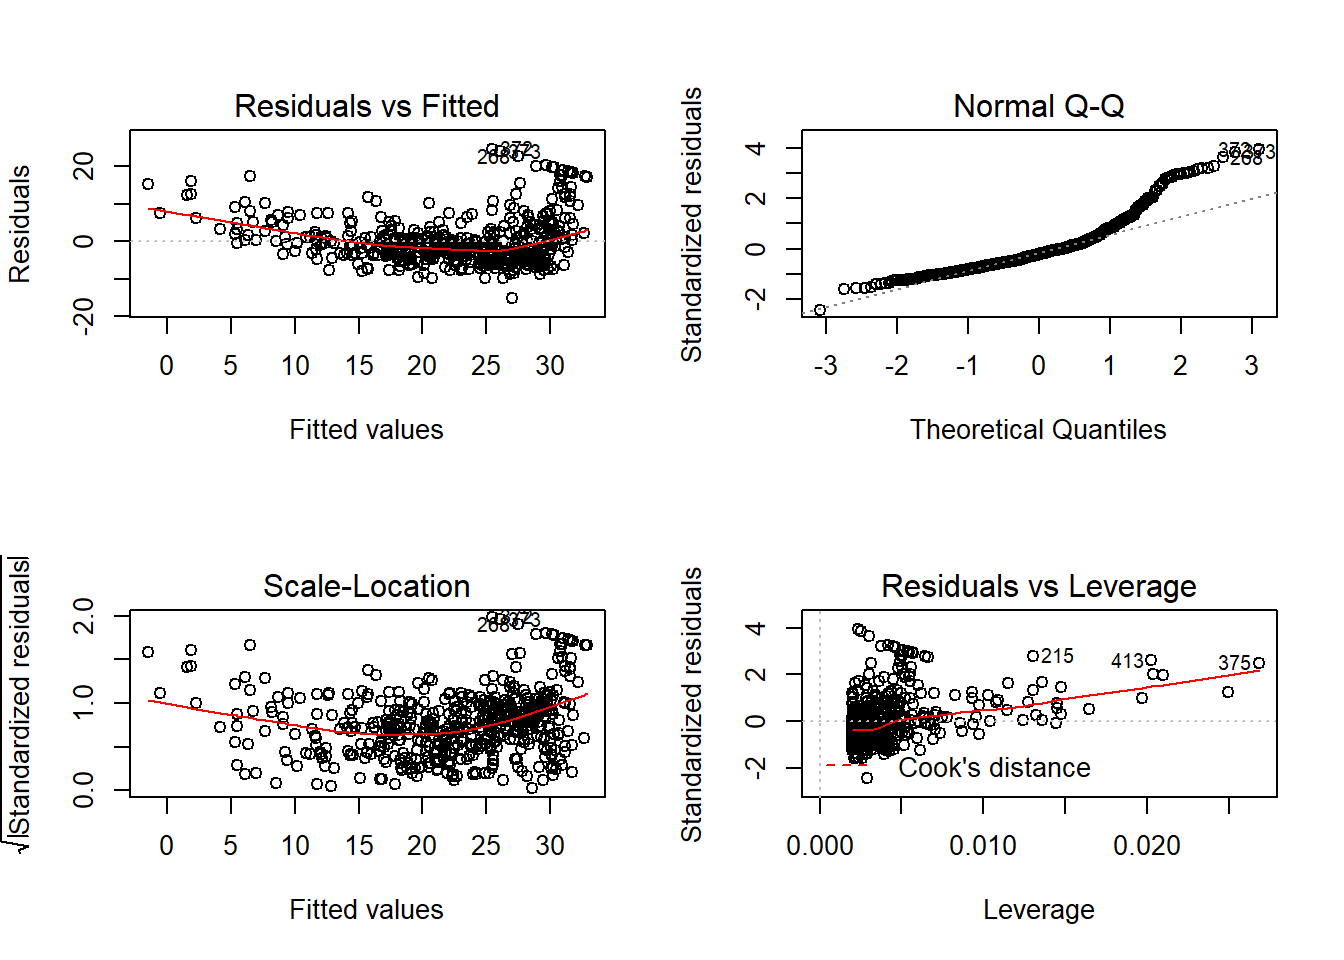
\includegraphics{02-Evaluation_files/figure-latex/unnamed-chunk-20-1.pdf}

\begin{itemize}
\tightlist
\item
  Utilizamos una medida \emph{robusta} (depende de la mediana y del IQR\footnote{The interquartile range of an observation variable is the difference of its upper and lower quartiles. It is a measure of how far apart the middle portion of data spreads in value}) para segmentar los datos en dos clases:
\item
  \texttt{1} si las pérdidas son atípicamente altas o
\item
  \texttt{0} si no lo son.
\end{itemize}

\begin{Shaded}
\begin{Highlighting}[]
\NormalTok{lsup <-}\StringTok{ }\KeywordTok{median}\NormalTok{(LOSS) }\OperatorTok{+}\StringTok{ }\FloatTok{1.5}\OperatorTok{*}\KeywordTok{IQR}\NormalTok{(LOSS) }\CommentTok{# Criterio basado en estadisticos robustos}
\KeywordTok{sum}\NormalTok{(LOSS}\OperatorTok{>=}\NormalTok{lsup) }\CommentTok{# 153 datos de perdidas atipicamente altas}
\end{Highlighting}
\end{Shaded}

\begin{verbatim}
FALSE [1] 153
\end{verbatim}

\begin{itemize}
\tightlist
\item
  (Opcional) Guardamos el gráfico del histograma de las \textbf{pérdidas no severas}
\end{itemize}

\begin{Shaded}
\begin{Highlighting}[]
\NormalTok{  Path_to_graphics <-}\StringTok{ }\KeywordTok{paste0}\NormalTok{(}\KeywordTok{getwd}\NormalTok{(),}\StringTok{"/"}\NormalTok{,}\StringTok{"Graphics"}\NormalTok{)}
  \KeywordTok{dir.create}\NormalTok{(Path_to_graphics)}
  \KeywordTok{png}\NormalTok{(}\KeywordTok{paste0}\NormalTok{(Path_to_graphics,}\StringTok{"/histograma.png"}\NormalTok{))}
  \KeywordTok{hist}\NormalTok{(LOSS[LOSS}\OperatorTok{<}\NormalTok{lsup], }\DataTypeTok{breaks =} \DecValTok{100}\NormalTok{, }\DataTypeTok{probability =}\NormalTok{ T, }\DataTypeTok{xlab=}\StringTok{"loss (pérdida en miles US $)"}\NormalTok{, }\DataTypeTok{main=}\StringTok{"Pérdida no severa"}\NormalTok{)}
  \KeywordTok{lines}\NormalTok{(}\KeywordTok{density}\NormalTok{(LOSS[LOSS}\OperatorTok{<}\NormalTok{lsup]),}\DataTypeTok{col=}\StringTok{"red"}\NormalTok{)}
  \KeywordTok{dev.off}\NormalTok{()}
\end{Highlighting}
\end{Shaded}

\begin{verbatim}
FALSE pdf 
FALSE   2
\end{verbatim}

\begin{quote}
Creamos el \emph{dataset} de trabajo.
\end{quote}

\begin{itemize}
\tightlist
\item
  Creamos un dataset o tabla de trabajo eliminando la variable CASENUM (id) y filtrando por la variable LOSS y el valor lsup= 72.22587 (miles).
\end{itemize}

\begin{Shaded}
\begin{Highlighting}[]
\NormalTok{df_autobi <-}\StringTok{ }\NormalTok{AutoBi[ , }\OperatorTok{-}\KeywordTok{match}\NormalTok{(}\StringTok{"CASENUM"}\NormalTok{, }\KeywordTok{colnames}\NormalTok{(AutoBi)) ] }
\end{Highlighting}
\end{Shaded}

\begin{itemize}
\item
  Fijamos los predictores categóricos como factores:

  \begin{itemize}
  \tightlist
  \item
    Representado por un abogado: `1' = representado por letrado y `2' = no representado
  \end{itemize}
\end{itemize}

\begin{Shaded}
\begin{Highlighting}[]
\NormalTok{  df_autobi}\OperatorTok{$}\NormalTok{ATTORNEY <-}\StringTok{ }\KeywordTok{ordered}\NormalTok{(df_autobi}\OperatorTok{$}\NormalTok{ATTORNEY, }\DataTypeTok{levels =} \DecValTok{1}\OperatorTok{:}\DecValTok{2}\NormalTok{) }
\end{Highlighting}
\end{Shaded}

\begin{itemize}
\tightlist
\item
  Sexo: `1' = hombre y `2' = mujer
\end{itemize}

\begin{Shaded}
\begin{Highlighting}[]
\NormalTok{  df_autobi}\OperatorTok{$}\NormalTok{CLMSEX   <-}\StringTok{ }\KeywordTok{ordered}\NormalTok{(df_autobi}\OperatorTok{$}\NormalTok{CLMSEX  , }\DataTypeTok{levels =} \DecValTok{1}\OperatorTok{:}\DecValTok{2}\NormalTok{)}
\end{Highlighting}
\end{Shaded}

\begin{itemize}
\tightlist
\item
  Estado civil: `1' = casado, `2' = soltero, `3' = viudo y `4' = divorciado / separado
\end{itemize}

\begin{Shaded}
\begin{Highlighting}[]
\NormalTok{  df_autobi}\OperatorTok{$}\NormalTok{MARITAL  <-}\StringTok{ }\KeywordTok{ordered}\NormalTok{(df_autobi}\OperatorTok{$}\NormalTok{MARITAL , }\DataTypeTok{levels =} \DecValTok{1}\OperatorTok{:}\DecValTok{4}\NormalTok{)}
\end{Highlighting}
\end{Shaded}

\begin{itemize}
\tightlist
\item
  Vehículo asegurado: `1' = vehículo estaba asegurado y `2'= no lo estaba
\end{itemize}

\begin{Shaded}
\begin{Highlighting}[]
\NormalTok{  df_autobi}\OperatorTok{$}\NormalTok{CLMINSUR <-}\StringTok{ }\KeywordTok{ordered}\NormalTok{(df_autobi}\OperatorTok{$}\NormalTok{CLMINSUR, }\DataTypeTok{levels =} \DecValTok{1}\OperatorTok{:}\DecValTok{2}\NormalTok{) }
\end{Highlighting}
\end{Shaded}

\begin{itemize}
\tightlist
\item
  Cinturón de seguridad: `1' = llevaba cinturón abrochado y `2' = no lo llevaba
\end{itemize}

\begin{Shaded}
\begin{Highlighting}[]
\NormalTok{  df_autobi}\OperatorTok{$}\NormalTok{SEATBELT <-}\StringTok{ }\KeywordTok{ordered}\NormalTok{(df_autobi}\OperatorTok{$}\NormalTok{SEATBELT, }\DataTypeTok{levels =} \DecValTok{1}\OperatorTok{:}\DecValTok{2}\NormalTok{)}
\end{Highlighting}
\end{Shaded}

\begin{itemize}
\tightlist
\item
  Pérdida: `1'= pérdida severa y `2'= pérdida no severa
\end{itemize}

\begin{Shaded}
\begin{Highlighting}[]
\NormalTok{df_autobi}\OperatorTok{$}\NormalTok{Y        <-}\StringTok{ }\KeywordTok{ifelse}\NormalTok{(df_autobi}\OperatorTok{$}\NormalTok{LOSS}\OperatorTok{>=}\StringTok{ }\NormalTok{lsup,}\DecValTok{1}\NormalTok{,}\DecValTok{0}\NormalTok{)}
\end{Highlighting}
\end{Shaded}

\begin{itemize}
\tightlist
\item
  Exploramos el \emph{dataset} que acabamos de crear y verificamos la proporción de casos con pérdida severa (11.42\%)
\end{itemize}

\begin{Shaded}
\begin{Highlighting}[]
\KeywordTok{summary}\NormalTok{(df_autobi)}
\end{Highlighting}
\end{Shaded}

\begin{verbatim}
FALSE  ATTORNEY  CLMSEX    MARITAL    CLMINSUR    SEATBELT        CLMAGE     
FALSE  1:685    1   :586   1   :624   1   : 120   1   :1270   Min.   : 0.00  
FALSE  2:655    2   :742   2   :650   2   :1179   2   :  22   1st Qu.:19.00  
FALSE           NA's: 12   3   : 15   NA's:  41   NA's:  48   Median :31.00  
FALSE                      4   : 35                           Mean   :32.53  
FALSE                      NA's: 16                           3rd Qu.:43.00  
FALSE                                                         Max.   :95.00  
FALSE                                                         NA's   :189    
FALSE       LOSS                Y         
FALSE  Min.   :   0.005   Min.   :0.0000  
FALSE  1st Qu.:   0.640   1st Qu.:0.0000  
FALSE  Median :   2.331   Median :0.0000  
FALSE  Mean   :   5.954   Mean   :0.1142  
FALSE  3rd Qu.:   3.995   3rd Qu.:0.0000  
FALSE  Max.   :1067.697   Max.   :1.0000  
FALSE 
\end{verbatim}

\begin{itemize}
\tightlist
\item
  Exploramos la relación de la pérdida con los factores.
\end{itemize}

\begin{Shaded}
\begin{Highlighting}[]
\NormalTok{agg_loss_attorney <-}\StringTok{ }\KeywordTok{aggregate}\NormalTok{(LOSS, }\DataTypeTok{by =} \KeywordTok{list}\NormalTok{(ATTORNEY) , }\DataTypeTok{FUN=}\NormalTok{ mean , }\DataTypeTok{na.rm=}\OtherTok{TRUE}\NormalTok{)}
  \KeywordTok{dimnames}\NormalTok{(agg_loss_attorney)[[}\DecValTok{1}\NormalTok{]] <-}\StringTok{ }\KeywordTok{c}\NormalTok{(}\StringTok{"REPRESENTED"}\NormalTok{,}\StringTok{"NOT REPRESENTED"}\NormalTok{) ; }\KeywordTok{dimnames}\NormalTok{(agg_loss_attorney)[[}\DecValTok{2}\NormalTok{]] <-}\StringTok{ }\KeywordTok{c}\NormalTok{(}\StringTok{"ATTORNEY"}\NormalTok{,}\StringTok{"LOSS"}\NormalTok{)}
  
\NormalTok{  agg_loss_clmsex   <-}\StringTok{ }\KeywordTok{aggregate}\NormalTok{(LOSS, }\DataTypeTok{by =} \KeywordTok{list}\NormalTok{(CLMSEX)  , }\DataTypeTok{FUN=}\NormalTok{ mean , }\DataTypeTok{na.rm=}\OtherTok{TRUE}\NormalTok{)}
  \KeywordTok{dimnames}\NormalTok{(agg_loss_clmsex)[[}\DecValTok{1}\NormalTok{]]   <-}\StringTok{ }\KeywordTok{c}\NormalTok{(}\StringTok{"MALE"}\NormalTok{,}\StringTok{"FEMALE"}\NormalTok{)  ; }\KeywordTok{dimnames}\NormalTok{(agg_loss_clmsex)[[}\DecValTok{2}\NormalTok{]] <-}\StringTok{ }\KeywordTok{c}\NormalTok{(}\StringTok{"CLMSEX"}\NormalTok{,}\StringTok{"LOSS"}\NormalTok{)}
  
\NormalTok{  agg_loss_marital  <-}\StringTok{ }\KeywordTok{aggregate}\NormalTok{(LOSS, }\DataTypeTok{by =} \KeywordTok{list}\NormalTok{(MARITAL) , }\DataTypeTok{FUN=}\NormalTok{ mean , }\DataTypeTok{na.rm=}\OtherTok{TRUE}\NormalTok{)}
  \KeywordTok{dimnames}\NormalTok{(agg_loss_marital)[[}\DecValTok{1}\NormalTok{]]  <-}\StringTok{ }\KeywordTok{c}\NormalTok{(}\StringTok{"MARRIED"}\NormalTok{,}\StringTok{"SINGLE"}\NormalTok{,}\StringTok{"WIDOW"}\NormalTok{,}\StringTok{"DIVORCED"}\NormalTok{) ; }\KeywordTok{dimnames}\NormalTok{(agg_loss_marital)[[}\DecValTok{2}\NormalTok{]] <-}\StringTok{ }\KeywordTok{c}\NormalTok{(}\StringTok{"MARITAL"}\NormalTok{,}\StringTok{"LOSS"}\NormalTok{)}
  
\NormalTok{  agg_loss_clminsur <-}\StringTok{ }\KeywordTok{aggregate}\NormalTok{(LOSS, }\DataTypeTok{by =} \KeywordTok{list}\NormalTok{(CLMINSUR) , }\DataTypeTok{FUN=}\NormalTok{ mean , }\DataTypeTok{na.rm=}\OtherTok{TRUE}\NormalTok{)}
  \KeywordTok{dimnames}\NormalTok{(agg_loss_clminsur)[[}\DecValTok{1}\NormalTok{]] <-}\StringTok{ }\KeywordTok{c}\NormalTok{(}\StringTok{"INSURED"}\NormalTok{,}\StringTok{"NOT INSURED"}\NormalTok{) ; }\KeywordTok{dimnames}\NormalTok{(agg_loss_clminsur)[[}\DecValTok{2}\NormalTok{]] <-}\StringTok{ }\KeywordTok{c}\NormalTok{(}\StringTok{"CLMINSUR"}\NormalTok{,}\StringTok{"LOSS"}\NormalTok{)}
  
\NormalTok{  agg_loss_seatbelt <-}\StringTok{ }\KeywordTok{aggregate}\NormalTok{(LOSS, }\DataTypeTok{by =} \KeywordTok{list}\NormalTok{(SEATBELT) , }\DataTypeTok{FUN=}\NormalTok{ mean , }\DataTypeTok{na.rm=}\OtherTok{TRUE}\NormalTok{)}
  \KeywordTok{dimnames}\NormalTok{(agg_loss_seatbelt)[[}\DecValTok{1}\NormalTok{]] <-}\StringTok{ }\KeywordTok{c}\NormalTok{(}\StringTok{"SEATBELT"}\NormalTok{,}\StringTok{"NOT SEATBELT"}\NormalTok{) ; }\KeywordTok{dimnames}\NormalTok{(agg_loss_seatbelt)[[}\DecValTok{2}\NormalTok{]] <-}\StringTok{ }\KeywordTok{c}\NormalTok{(}\StringTok{"SEATBELT"}\NormalTok{,}\StringTok{"LOSS"}\NormalTok{)}
\end{Highlighting}
\end{Shaded}

\begin{quote}
Creamos los sets \emph{train} y \emph{test}
\end{quote}

\begin{itemize}
\tightlist
\item
  Aleatorizamos los datos y separamos el set de datos en \emph{train} y \emph{test}:
\end{itemize}

\begin{Shaded}
\begin{Highlighting}[]
\NormalTok{N=}\KeywordTok{nrow}\NormalTok{(df_autobi)}
\end{Highlighting}
\end{Shaded}

\begin{itemize}
\tightlist
\item
  Es recomendable fijar una semilla (seed) para los algoritmos de aleatorización internos de R
\end{itemize}

\begin{Shaded}
\begin{Highlighting}[]
\ControlFlowTok{if}\NormalTok{ (}\OperatorTok{!}\KeywordTok{require}\NormalTok{(caret)) }\KeywordTok{install.packages}\NormalTok{(}\StringTok{'caret'}\NormalTok{)}
\KeywordTok{library}\NormalTok{(caret)  }
\KeywordTok{set.seed}\NormalTok{(}\DecValTok{123456}\NormalTok{)}
\NormalTok{inTrain  <-}\StringTok{ }\KeywordTok{createDataPartition}\NormalTok{(df_autobi}\OperatorTok{$}\NormalTok{Y, }\DataTypeTok{times =} \DecValTok{1}\NormalTok{, }\DataTypeTok{p =} \FloatTok{0.7}\NormalTok{, }\DataTypeTok{list =} \OtherTok{TRUE}\NormalTok{)}
\NormalTok{dt_train <-}\StringTok{ }\NormalTok{df_autobi[inTrain[[}\DecValTok{1}\NormalTok{]],]  }\CommentTok{# 938 casos}
\NormalTok{dt_test  <-}\StringTok{ }\NormalTok{df_autobi[}\OperatorTok{-}\NormalTok{inTrain[[}\DecValTok{1}\NormalTok{]],] }\CommentTok{# 402 casos}
  
\KeywordTok{nrow}\NormalTok{(dt_train)}
\end{Highlighting}
\end{Shaded}

\begin{verbatim}
FALSE [1] 938
\end{verbatim}

\begin{Shaded}
\begin{Highlighting}[]
\KeywordTok{summary}\NormalTok{(dt_train)}
\end{Highlighting}
\end{Shaded}

\begin{verbatim}
FALSE  ATTORNEY  CLMSEX    MARITAL    CLMINSUR   SEATBELT       CLMAGE     
FALSE  1:471    1   :406   1   :439   1   : 77   1   :885   Min.   : 0.00  
FALSE  2:467    2   :523   2   :455   2   :833   2   : 17   1st Qu.:20.00  
FALSE           NA's:  9   3   : 10   NA's: 28   NA's: 36   Median :32.00  
FALSE                      4   : 25                         Mean   :33.06  
FALSE                      NA's:  9                         3rd Qu.:43.00  
FALSE                                                       Max.   :95.00  
FALSE                                                       NA's   :134    
FALSE       LOSS                Y         
FALSE  Min.   :  0.0050   Min.   :0.0000  
FALSE  1st Qu.:  0.7123   1st Qu.:0.0000  
FALSE  Median :  2.3645   Median :0.0000  
FALSE  Mean   :  5.4656   Mean   :0.1141  
FALSE  3rd Qu.:  4.0263   3rd Qu.:0.0000  
FALSE  Max.   :273.6040   Max.   :1.0000  
FALSE 
\end{verbatim}

\begin{Shaded}
\begin{Highlighting}[]
\KeywordTok{nrow}\NormalTok{(dt_test)}
\end{Highlighting}
\end{Shaded}

\begin{verbatim}
FALSE [1] 402
\end{verbatim}

\begin{Shaded}
\begin{Highlighting}[]
\KeywordTok{summary}\NormalTok{(dt_test)}
\end{Highlighting}
\end{Shaded}

\begin{verbatim}
FALSE  ATTORNEY  CLMSEX    MARITAL    CLMINSUR   SEATBELT       CLMAGE     
FALSE  1:214    1   :180   1   :185   1   : 43   1   :385   Min.   : 0.00  
FALSE  2:188    2   :219   2   :195   2   :346   2   :  5   1st Qu.:19.00  
FALSE           NA's:  3   3   :  5   NA's: 13   NA's: 12   Median :29.00  
FALSE                      4   : 10                         Mean   :31.31  
FALSE                      NA's:  7                         3rd Qu.:42.00  
FALSE                                                       Max.   :78.00  
FALSE                                                       NA's   :55     
FALSE       LOSS                 Y         
FALSE  Min.   :   0.0050   Min.   :0.0000  
FALSE  1st Qu.:   0.5175   1st Qu.:0.0000  
FALSE  Median :   2.1645   Median :0.0000  
FALSE  Mean   :   7.0917   Mean   :0.1144  
FALSE  3rd Qu.:   3.7782   3rd Qu.:0.0000  
FALSE  Max.   :1067.6970   Max.   :1.0000  
FALSE 
\end{verbatim}

Comprobamos si se que los conjuntos train y test se han formado correctamente

\begin{Shaded}
\begin{Highlighting}[]
  \KeywordTok{length}\NormalTok{(}\KeywordTok{intersect}\NormalTok{(inTrain, }\KeywordTok{setdiff}\NormalTok{(}\DecValTok{1}\OperatorTok{:}\NormalTok{N,inTrain)))}
\end{Highlighting}
\end{Shaded}

\begin{verbatim}
FALSE [1] 0
\end{verbatim}

\hypertarget{clasificacion-1}{%
\subsection{Clasificación}\label{clasificacion-1}}

Vamos a construir un modelo para identificar los casos con pérdidas severas.

\begin{itemize}
\tightlist
\item
  El primer ejemplo lo hacemos con \emph{Random Forest}
\end{itemize}

\begin{Shaded}
\begin{Highlighting}[]
\ControlFlowTok{if}\NormalTok{ (}\OperatorTok{!}\KeywordTok{require}\NormalTok{(randomForest)) }\KeywordTok{install.packages}\NormalTok{(}\StringTok{'randomForest'}\NormalTok{)}
\KeywordTok{library}\NormalTok{(randomForest)}
\end{Highlighting}
\end{Shaded}

\begin{itemize}
\tightlist
\item
  Creamos un objeto de clase `formula' y se lo pasamos como argumento a la función \texttt{randomForest}\footnote{\url{https://www.rdocumentation.org/packages/randomForest/versions/4.6-12/topics/randomForest}}
\end{itemize}

\begin{Shaded}
\begin{Highlighting}[]
\KeywordTok{set.seed}\NormalTok{(}\DecValTok{123456}\NormalTok{)}
\NormalTok{fmla.rf1 <-}\StringTok{ }\KeywordTok{as.formula}\NormalTok{(}\KeywordTok{paste0}\NormalTok{(}\StringTok{"Y"}\NormalTok{,}\StringTok{" ~"}\NormalTok{,}\KeywordTok{paste0}\NormalTok{(}\KeywordTok{colnames}\NormalTok{(df_autobi[,}\OperatorTok{-}\KeywordTok{c}\NormalTok{(}\DecValTok{7}\NormalTok{,}\DecValTok{8}\NormalTok{)]),}\DataTypeTok{collapse =} \StringTok{"+"}\NormalTok{),}\DataTypeTok{collapse =} \StringTok{""}\NormalTok{))}
\NormalTok{rf1 <-}\StringTok{ }\KeywordTok{randomForest}\NormalTok{( fmla.rf1,}
                       \DataTypeTok{data =}\NormalTok{dt_train,}
                       \DataTypeTok{ntree =} \DecValTok{5000}\NormalTok{, }\CommentTok{# se ejecuta muy rapido, podemos utilizar ntree > = 2500}
                       \DataTypeTok{replace =}\OtherTok{TRUE}\NormalTok{,}
                       \DataTypeTok{mtry=}\DecValTok{4}\NormalTok{,}
                       \DataTypeTok{maxnodes =}\DecValTok{50}\NormalTok{,}
                       \DataTypeTok{importance =} \OtherTok{TRUE}\NormalTok{,}
                       \DataTypeTok{proximity =}   \OtherTok{TRUE}\NormalTok{,}
                       \DataTypeTok{keep.forest =} \OtherTok{TRUE}\NormalTok{,}
                       \DataTypeTok{na.action=}\NormalTok{na.omit)}
\end{Highlighting}
\end{Shaded}

\begin{itemize}
\tightlist
\item
  Exploramos el objeto con los resutados
\end{itemize}

\begin{Shaded}
\begin{Highlighting}[]
\NormalTok{rf1}
\end{Highlighting}
\end{Shaded}

\begin{verbatim}
FALSE 
FALSE Call:
FALSE  randomForest(formula = fmla.rf1, data = dt_train, ntree = 5000,      replace = TRUE, mtry = 4, maxnodes = 50, importance = TRUE,      proximity = TRUE, keep.forest = TRUE, na.action = na.omit) 
FALSE                Type of random forest: regression
FALSE                      Number of trees: 5000
FALSE No. of variables tried at each split: 4
FALSE 
FALSE           Mean of squared residuals: 0.1009875
FALSE                     % Var explained: 4.3
\end{verbatim}

\begin{Shaded}
\begin{Highlighting}[]
\KeywordTok{summary}\NormalTok{(rf1)}
\end{Highlighting}
\end{Shaded}

\begin{verbatim}
FALSE                 Length Class  Mode     
FALSE call                11 -none- call     
FALSE type                 1 -none- character
FALSE predicted          759 -none- numeric  
FALSE mse               5000 -none- numeric  
FALSE rsq               5000 -none- numeric  
FALSE oob.times          759 -none- numeric  
FALSE importance          12 -none- numeric  
FALSE importanceSD         6 -none- numeric  
FALSE localImportance      0 -none- NULL     
FALSE proximity       576081 -none- numeric  
FALSE ntree                1 -none- numeric  
FALSE mtry                 1 -none- numeric  
FALSE forest              11 -none- list     
FALSE coefs                0 -none- NULL     
FALSE y                  759 -none- numeric  
FALSE test                 0 -none- NULL     
FALSE inbag                0 -none- NULL     
FALSE terms                3 terms  call     
FALSE na.action          179 omit   numeric
\end{verbatim}

\begin{Shaded}
\begin{Highlighting}[]
\KeywordTok{str}\NormalTok{(rf1)}
\end{Highlighting}
\end{Shaded}

\begin{verbatim}
FALSE List of 19
FALSE  $ call           : language randomForest(formula = fmla.rf1, data = dt_train, ntree = 5000, replace = TRUE,      mtry = 4, maxnodes = 50, imp| __truncated__ ...
FALSE  $ type           : chr "regression"
FALSE  $ predicted      : Named num [1:759] 0.00767 0.000161 0.629748 0.008208 0.022047 ...
FALSE   ..- attr(*, "names")= chr [1:759] "2" "3" "4" "5" ...
FALSE   ..- attr(*, "na.action")= 'omit' Named int [1:179] 1 9 19 25 27 40 43 46 50 51 ...
FALSE   .. ..- attr(*, "names")= chr [1:179] "1" "10" "24" "30" ...
FALSE  $ mse            : num [1:5000] 0.102 0.129 0.121 0.115 0.113 ...
FALSE  $ rsq            : num [1:5000] 0.0302 -0.2272 -0.1473 -0.0907 -0.071 ...
FALSE  $ oob.times      : int [1:759] 1804 1942 1844 1864 1855 1780 1837 1782 1847 1807 ...
FALSE  $ importance     : num [1:6, 1:2] 0.017697 -0.001602 0.004106 0.000933 0.0009 ...
FALSE   ..- attr(*, "dimnames")=List of 2
FALSE   .. ..$ : chr [1:6] "ATTORNEY" "CLMSEX" "MARITAL" "CLMINSUR" ...
FALSE   .. ..$ : chr [1:2] "%IncMSE" "IncNodePurity"
FALSE  $ importanceSD   : Named num [1:6] 1.50e-04 8.42e-05 1.54e-04 8.18e-05 5.65e-05 ...
FALSE   ..- attr(*, "names")= chr [1:6] "ATTORNEY" "CLMSEX" "MARITAL" "CLMINSUR" ...
FALSE  $ localImportance: NULL
FALSE  $ proximity      : num [1:759, 1:759] 1 0.179 0 0.318 0 ...
FALSE   ..- attr(*, "dimnames")=List of 2
FALSE   .. ..$ : chr [1:759] "2" "3" "4" "5" ...
FALSE   .. ..$ : chr [1:759] "2" "3" "4" "5" ...
FALSE  $ ntree          : num 5000
FALSE  $ mtry           : num 4
FALSE  $ forest         :List of 11
FALSE   ..$ ndbigtree    : int [1:5000] 99 99 99 99 99 99 99 99 99 99 ...
FALSE   ..$ nodestatus   : int [1:99, 1:5000] -3 -3 -3 -3 -3 -3 -3 -3 -3 -3 ...
FALSE   ..$ leftDaughter : int [1:99, 1:5000] 2 4 6 8 10 12 14 16 18 20 ...
FALSE   ..$ rightDaughter: int [1:99, 1:5000] 3 5 7 9 11 13 15 17 19 21 ...
FALSE   ..$ nodepred     : num [1:99, 1:5000] 0.1265 0.2198 0.0363 0.0115 0.2832 ...
FALSE   ..$ bestvar      : int [1:99, 1:5000] 1 6 4 6 5 6 6 6 6 3 ...
FALSE   ..$ xbestsplit   : num [1:99, 1:5000] 1.5 20.5 1.5 15.5 1.5 27.5 34.5 0 16.5 3.5 ...
FALSE   ..$ ncat         : Named int [1:6] 1 1 1 1 1 1
FALSE   .. ..- attr(*, "names")= chr [1:6] "ATTORNEY" "CLMSEX" "MARITAL" "CLMINSUR" ...
FALSE   ..$ nrnodes      : int 99
FALSE   ..$ ntree        : num 5000
FALSE   ..$ xlevels      :List of 6
FALSE   .. ..$ ATTORNEY: num 0
FALSE   .. ..$ CLMSEX  : num 0
FALSE   .. ..$ MARITAL : num 0
FALSE   .. ..$ CLMINSUR: num 0
FALSE   .. ..$ SEATBELT: num 0
FALSE   .. ..$ CLMAGE  : num 0
FALSE  $ coefs          : NULL
FALSE  $ y              : Named num [1:759] 1 0 1 0 0 0 0 0 0 1 ...
FALSE   ..- attr(*, "na.action")= 'omit' Named int [1:179] 1 9 19 25 27 40 43 46 50 51 ...
FALSE   .. ..- attr(*, "names")= chr [1:179] "1" "10" "24" "30" ...
FALSE   ..- attr(*, "names")= chr [1:759] "2" "3" "4" "5" ...
FALSE  $ test           : NULL
FALSE  $ inbag          : NULL
FALSE  $ terms          :Classes 'terms', 'formula'  language Y ~ ATTORNEY + CLMSEX + MARITAL + CLMINSUR + SEATBELT + CLMAGE
FALSE   .. ..- attr(*, "variables")= language list(Y, ATTORNEY, CLMSEX, MARITAL, CLMINSUR, SEATBELT, CLMAGE)
FALSE   .. ..- attr(*, "factors")= int [1:7, 1:6] 0 1 0 0 0 0 0 0 0 1 ...
FALSE   .. .. ..- attr(*, "dimnames")=List of 2
FALSE   .. .. .. ..$ : chr [1:7] "Y" "ATTORNEY" "CLMSEX" "MARITAL" ...
FALSE   .. .. .. ..$ : chr [1:6] "ATTORNEY" "CLMSEX" "MARITAL" "CLMINSUR" ...
FALSE   .. ..- attr(*, "term.labels")= chr [1:6] "ATTORNEY" "CLMSEX" "MARITAL" "CLMINSUR" ...
FALSE   .. ..- attr(*, "order")= int [1:6] 1 1 1 1 1 1
FALSE   .. ..- attr(*, "intercept")= num 0
FALSE   .. ..- attr(*, "response")= int 1
FALSE   .. ..- attr(*, ".Environment")=<environment: R_GlobalEnv> 
FALSE   .. ..- attr(*, "predvars")= language list(Y, ATTORNEY, CLMSEX, MARITAL, CLMINSUR, SEATBELT, CLMAGE)
FALSE   .. ..- attr(*, "dataClasses")= Named chr [1:7] "numeric" "ordered" "ordered" "ordered" ...
FALSE   .. .. ..- attr(*, "names")= chr [1:7] "Y" "ATTORNEY" "CLMSEX" "MARITAL" ...
FALSE  $ na.action      : 'omit' Named int [1:179] 1 9 19 25 27 40 43 46 50 51 ...
FALSE   ..- attr(*, "names")= chr [1:179] "1" "10" "24" "30" ...
FALSE  - attr(*, "class")= chr [1:2] "randomForest.formula" "randomForest"
\end{verbatim}

\begin{quote}
Gráfico de la importancia relativa de los predictores
\end{quote}

\begin{Shaded}
\begin{Highlighting}[]
  \KeywordTok{varImpPlot}\NormalTok{(rf1,}\DataTypeTok{sort =}\NormalTok{ T,}\DataTypeTok{main =} \StringTok{"Variable Importance"}\NormalTok{)}
\end{Highlighting}
\end{Shaded}

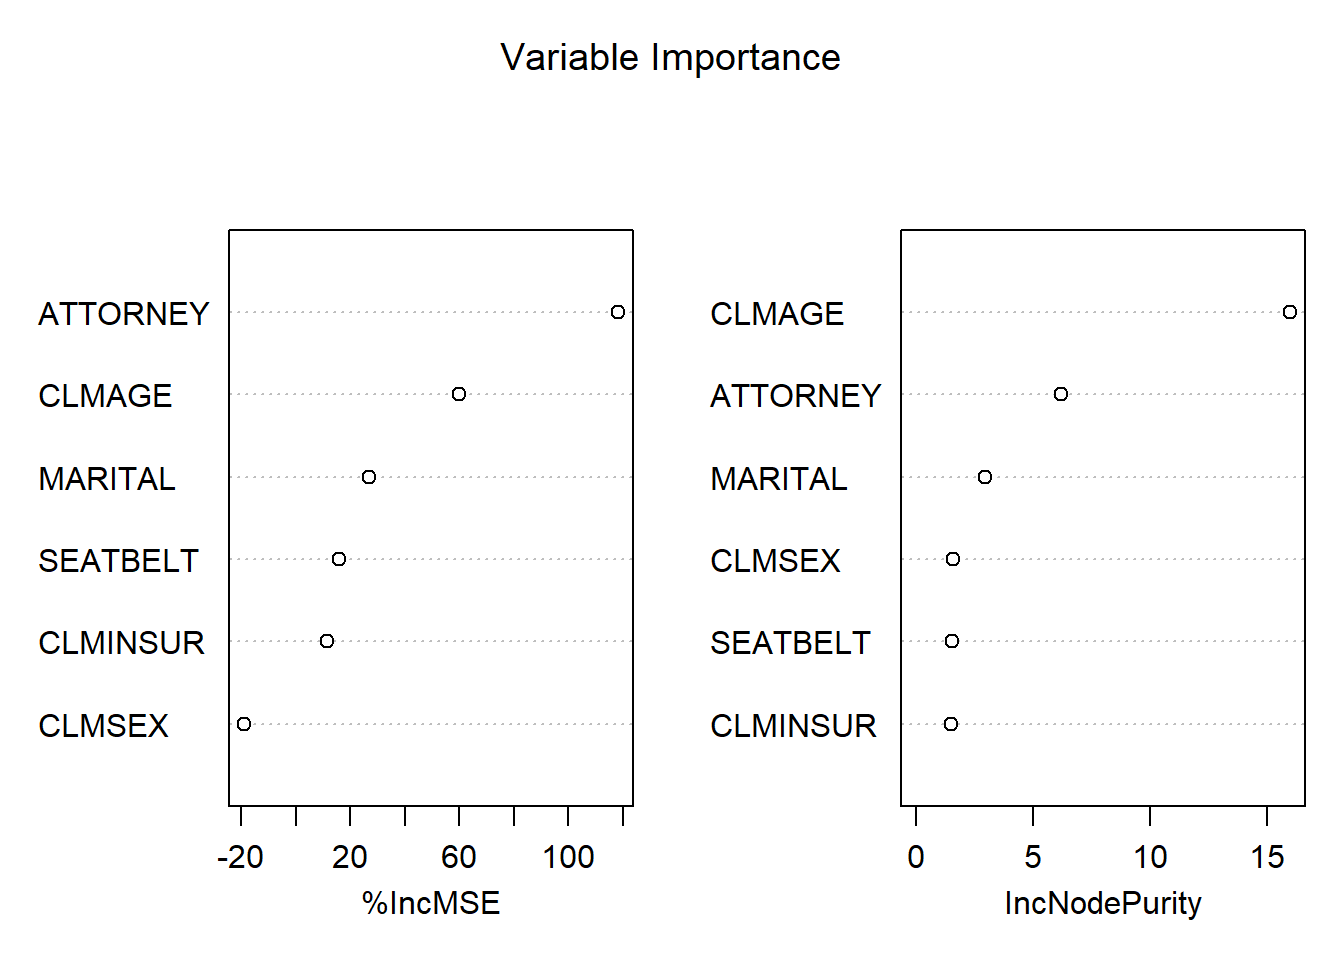
\includegraphics{02-Evaluation_files/figure-latex/unnamed-chunk-37-1.pdf}

\begin{quote}
Gráfico del Error vs número de árboles
\end{quote}

\begin{Shaded}
\begin{Highlighting}[]
  \KeywordTok{plot}\NormalTok{(rf1, }\DataTypeTok{main=}\StringTok{"Error de clasificación vs núero de  árboles"}\NormalTok{) }
\end{Highlighting}
\end{Shaded}

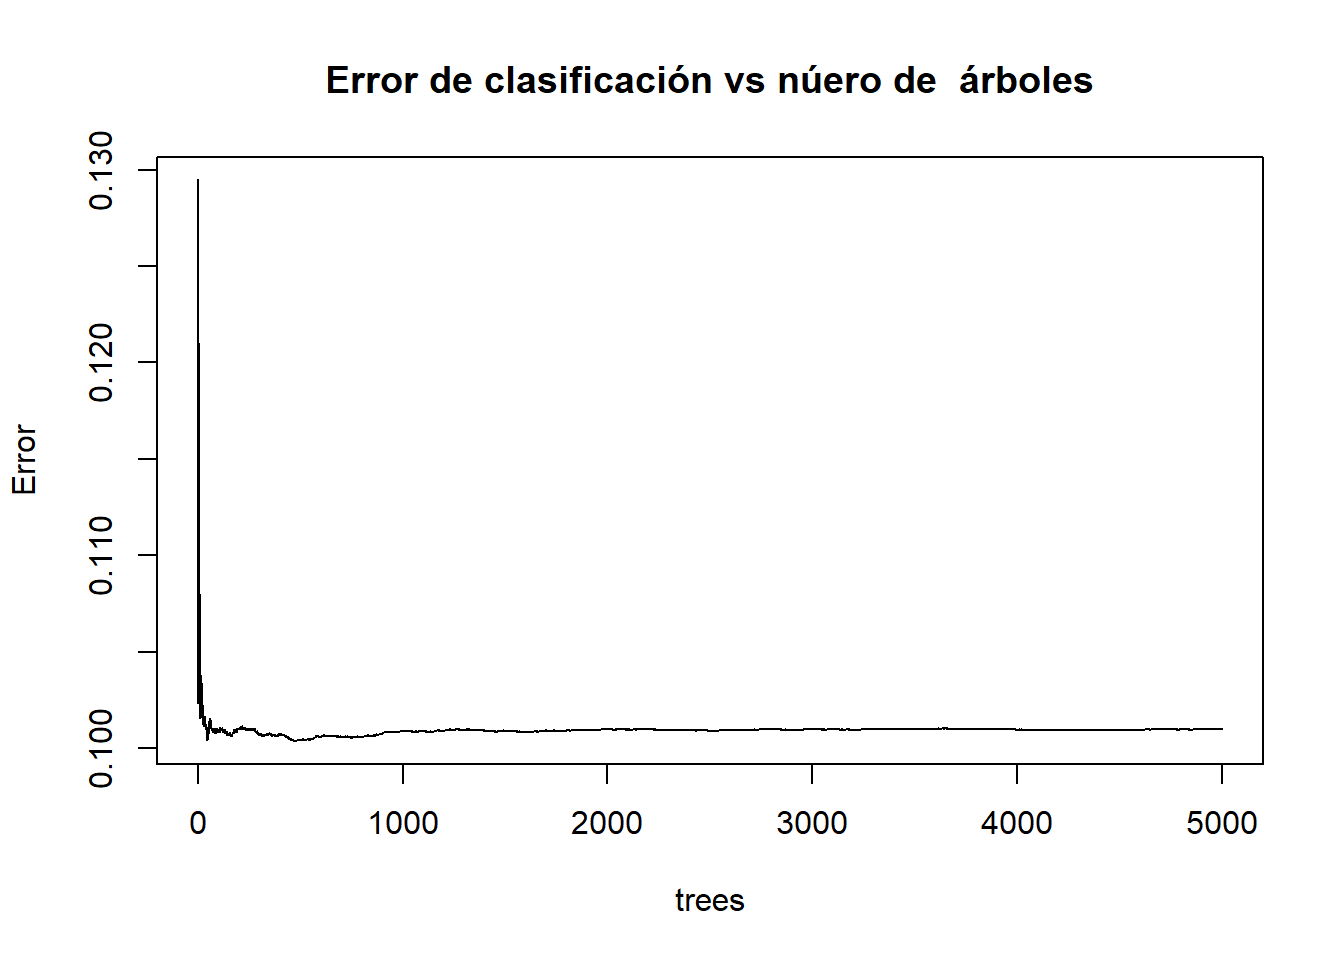
\includegraphics{02-Evaluation_files/figure-latex/unnamed-chunk-38-1.pdf}

\begin{quote}
Gráfico de la probabilidad condicional: \(P(Y=1|X_1 = ATTORNEY,\ldots,X_6=SEATBELT)\)
\end{quote}

\begin{Shaded}
\begin{Highlighting}[]
\NormalTok{  rf1.prediction <-}\StringTok{ }\KeywordTok{as.data.frame}\NormalTok{(}\KeywordTok{predict}\NormalTok{(rf1, }\DataTypeTok{newdata =}\NormalTok{ dt_train))}
  \KeywordTok{summary}\NormalTok{(rf1.prediction)}
\end{Highlighting}
\end{Shaded}

\begin{verbatim}
##  predict(rf1, newdata = dt_train)
##  Min.   :0.00005                 
##  1st Qu.:0.00599                 
##  Median :0.03651                 
##  Mean   :0.11984                 
##  3rd Qu.:0.21024                 
##  Max.   :0.77138                 
##  NA's   :179
\end{verbatim}

\begin{Shaded}
\begin{Highlighting}[]
\NormalTok{  dt_train}\OperatorTok{$}\NormalTok{pred_rf1 <-}\StringTok{ }\NormalTok{rf1.prediction}\OperatorTok{$}\StringTok{`}\DataTypeTok{predict(rf1, newdata = dt_train)}\StringTok{`} 
  \KeywordTok{head}\NormalTok{(dt_train,}\DecValTok{3}\NormalTok{)}
\end{Highlighting}
\end{Shaded}

\begin{verbatim}
##   ATTORNEY CLMSEX MARITAL CLMINSUR SEATBELT CLMAGE   LOSS Y     pred_rf1
## 1        1      1    <NA>        2        1     50 34.940 1           NA
## 2        2      2       2        1        1     28 10.892 1 0.3807199932
## 3        2      1       2        2        1      5  0.330 0 0.0001324938
\end{verbatim}

\begin{Shaded}
\begin{Highlighting}[]
  \KeywordTok{tail}\NormalTok{(dt_train,}\DecValTok{3}\NormalTok{)}
\end{Highlighting}
\end{Shaded}

\begin{verbatim}
##      ATTORNEY CLMSEX MARITAL CLMINSUR SEATBELT CLMAGE  LOSS Y    pred_rf1
## 1335        2      2       2        2        1     26 0.161 0 0.001142849
## 1338        2      2       1        2        1     39 0.099 0 0.012354460
## 1340        2      2       2        2        1     30 0.688 0 0.002329733
\end{verbatim}

\begin{Shaded}
\begin{Highlighting}[]
  \KeywordTok{summary}\NormalTok{(dt_train)}
\end{Highlighting}
\end{Shaded}

\begin{verbatim}
##  ATTORNEY  CLMSEX    MARITAL    CLMINSUR   SEATBELT       CLMAGE     
##  1:471    1   :406   1   :439   1   : 77   1   :885   Min.   : 0.00  
##  2:467    2   :523   2   :455   2   :833   2   : 17   1st Qu.:20.00  
##           NA's:  9   3   : 10   NA's: 28   NA's: 36   Median :32.00  
##                      4   : 25                         Mean   :33.06  
##                      NA's:  9                         3rd Qu.:43.00  
##                                                       Max.   :95.00  
##                                                       NA's   :134    
##       LOSS                Y             pred_rf1      
##  Min.   :  0.0050   Min.   :0.0000   Min.   :0.00005  
##  1st Qu.:  0.7123   1st Qu.:0.0000   1st Qu.:0.00599  
##  Median :  2.3645   Median :0.0000   Median :0.03651  
##  Mean   :  5.4656   Mean   :0.1141   Mean   :0.11984  
##  3rd Qu.:  4.0263   3rd Qu.:0.0000   3rd Qu.:0.21024  
##  Max.   :273.6040   Max.   :1.0000   Max.   :0.77138  
##                                      NA's   :179
\end{verbatim}

\begin{Shaded}
\begin{Highlighting}[]
  \KeywordTok{plot}\NormalTok{(}\KeywordTok{density}\NormalTok{(dt_train}\OperatorTok{$}\NormalTok{pred_rf1[}\OperatorTok{!}\KeywordTok{is.na}\NormalTok{(dt_train}\OperatorTok{$}\NormalTok{pred_rf1)]), }\DataTypeTok{col=}\StringTok{"red"}\NormalTok{ , }\DataTypeTok{xlab=}\StringTok{"Probabilidad"}\NormalTok{ , }\DataTypeTok{main=}\StringTok{"Función de densidad estimada"}\NormalTok{)}
\end{Highlighting}
\end{Shaded}

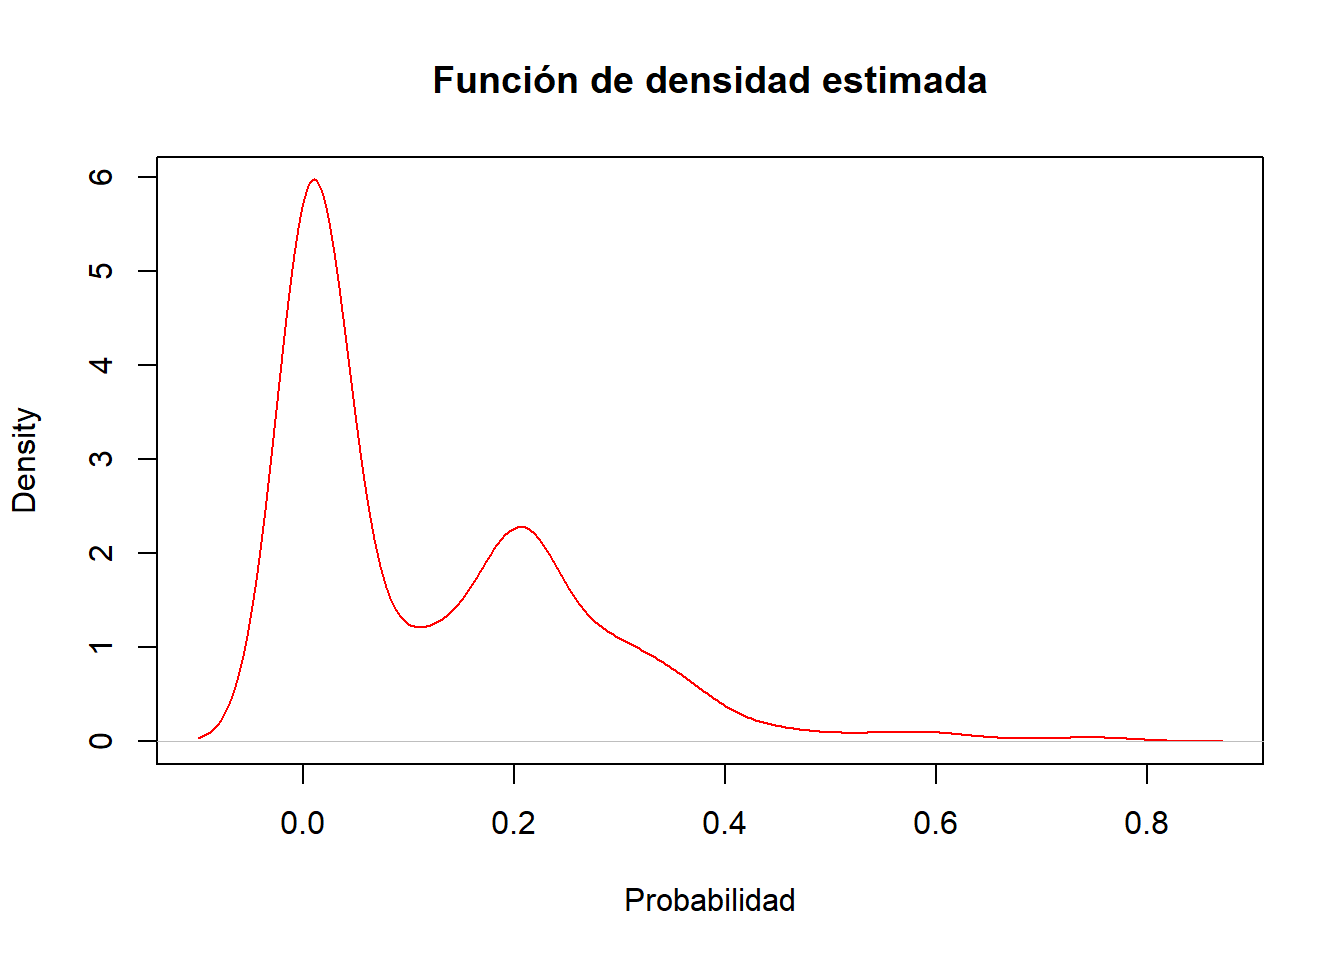
\includegraphics{02-Evaluation_files/figure-latex/unnamed-chunk-39-1.pdf}

\begin{itemize}
\item
  Vemos que hay (claramente) dos concentraciones (clases) de probabilidades de pérdida, una concentración en torno a la probabilidad de pérdida no severa (\(Y=0\)) y otra para la pérdida severa (\(Y=1\)).
\item
  Esto no lleva a la elección del \textbf{punto de corte óptimo} para obtener una regla de clasificación, es decir, un criterio para \(Y_{predicted}=1\) (pérdida severa), o bien, para \(Y_{predicted}=0\) (pérdida no severa). Una alternativa es el criterio de la \textbf{Distancia de Kolmogorov-Smirnov} (KS).
\end{itemize}

\begin{quote}
Métricas de evaluación del poder de clasificación
\end{quote}

\begin{Shaded}
\begin{Highlighting}[]
\ControlFlowTok{if}\NormalTok{ (}\OperatorTok{!}\KeywordTok{require}\NormalTok{(ModelMetrics)) }\KeywordTok{install.packages}\NormalTok{(}\StringTok{'ModelMetrics'}\NormalTok{)}
\KeywordTok{library}\NormalTok{(ModelMetrics)}
\ControlFlowTok{if}\NormalTok{ (}\OperatorTok{!}\KeywordTok{require}\NormalTok{(ROCR)) }\KeywordTok{install.packages}\NormalTok{(}\StringTok{'ROCR'}\NormalTok{)}
\KeywordTok{library}\NormalTok{(ROCR)}
\ControlFlowTok{if}\NormalTok{ (}\OperatorTok{!}\KeywordTok{require}\NormalTok{(binaryLogic)) }\KeywordTok{install.packages}\NormalTok{(}\StringTok{'binaryLogic'}\NormalTok{)}
\KeywordTok{library}\NormalTok{(binaryLogic)}
\end{Highlighting}
\end{Shaded}

\begin{itemize}
\tightlist
\item
  Con el train creamos un objeto de tipo `prediction'\footnote{\url{https://www.r-bloggers.com/a-small-introduction-to-the-rocr-package/}}
\end{itemize}

\begin{Shaded}
\begin{Highlighting}[]
\NormalTok{  rf1.pred <-}\StringTok{ }\KeywordTok{prediction}\NormalTok{(}\KeywordTok{as.numeric}\NormalTok{(rf1}\OperatorTok{$}\NormalTok{predicted),}\KeywordTok{as.numeric}\NormalTok{(rf1}\OperatorTok{$}\NormalTok{y)) }
\end{Highlighting}
\end{Shaded}

\begin{itemize}
\tightlist
\item
  Calculamos la Curva de ROC con la función `performance' sobre el objeto `rf1'
\end{itemize}

\begin{Shaded}
\begin{Highlighting}[]
\NormalTok{  rf1.perf <-}\StringTok{ }\KeywordTok{performance}\NormalTok{(rf1.pred,}\StringTok{"tpr"}\NormalTok{,}\StringTok{"fpr"}\NormalTok{) }
 \CommentTok{## "fpr" = False positive rate. P(Yhat = + | Y = -). Estimated as: FP/N.}
 \CommentTok{## "tpr" = True positive rate. P(Yhat = + | Y = +). Estimated as: TP/P.}
 \KeywordTok{plot}\NormalTok{(rf1.perf)}
\end{Highlighting}
\end{Shaded}

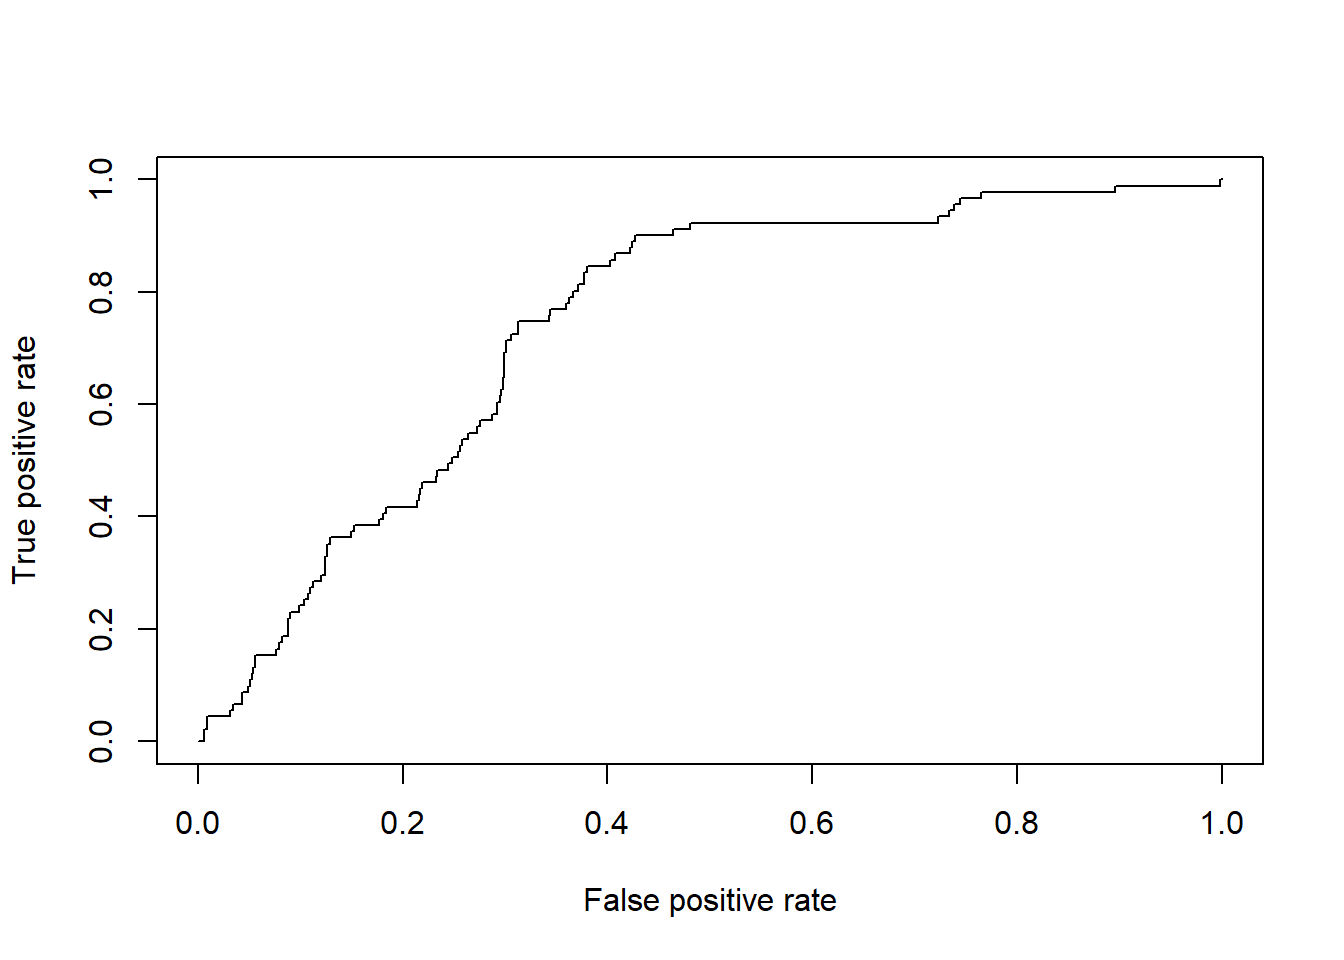
\includegraphics{02-Evaluation_files/figure-latex/unnamed-chunk-42-1.pdf}

\begin{quote}
Elección del punto de corte: Criterio de la distancia de KS
\end{quote}

\begin{itemize}
\tightlist
\item
  La distancia KS se calcula como: KS = abs(\href{mailto:rf1.perf@y.values}{\nolinkurl{rf1.perf@y.values}}{[}{[}1{]}{]}-\href{mailto:rf1.perf@x.values}{\nolinkurl{rf1.perf@x.values}}{[}{[}1{]}{]})
\end{itemize}

\begin{Shaded}
\begin{Highlighting}[]
\NormalTok{rf1.perf}\OperatorTok{@}\NormalTok{alpha.values[[}\DecValTok{1}\NormalTok{]][rf1.perf}\OperatorTok{@}\NormalTok{alpha.values[[}\DecValTok{1}\NormalTok{]]}\OperatorTok{==}\OtherTok{Inf}\NormalTok{] <-}\StringTok{ }\KeywordTok{round}\NormalTok{(}\KeywordTok{max}\NormalTok{(rf1.perf}\OperatorTok{@}\NormalTok{alpha.values[[}\DecValTok{1}\NormalTok{]][rf1.perf}\OperatorTok{@}\NormalTok{alpha.values[[}\DecValTok{1}\NormalTok{]]}\OperatorTok{!=}\OtherTok{Inf}\NormalTok{]),}\DecValTok{2}\NormalTok{)}
\NormalTok{KS.matrix=}\StringTok{ }\KeywordTok{cbind}\NormalTok{(}\KeywordTok{abs}\NormalTok{(rf1.perf}\OperatorTok{@}\NormalTok{y.values[[}\DecValTok{1}\NormalTok{]]}\OperatorTok{-}\NormalTok{rf1.perf}\OperatorTok{@}\NormalTok{x.values[[}\DecValTok{1}\NormalTok{]]), rf1.perf}\OperatorTok{@}\NormalTok{alpha.values[[}\DecValTok{1}\NormalTok{]])}
\end{Highlighting}
\end{Shaded}

\begin{itemize}
\tightlist
\item
  Resumiendo
\end{itemize}

\begin{Shaded}
\begin{Highlighting}[]
\KeywordTok{colnames}\NormalTok{(KS.matrix) <-}\StringTok{ }\KeywordTok{c}\NormalTok{(}\StringTok{"KS-distance"}\NormalTok{,}\StringTok{"cut-point"}\NormalTok{)}
\KeywordTok{head}\NormalTok{(KS.matrix)}
\end{Highlighting}
\end{Shaded}

\begin{verbatim}
##      KS-distance cut-point
## [1,] 0.000000000 0.7800000
## [2,] 0.001497006 0.7809184
## [3,] 0.002994012 0.7353170
## [4,] 0.004491018 0.6577091
## [5,] 0.005988024 0.6481896
## [6,] 0.005000987 0.6297476
\end{verbatim}

\begin{Shaded}
\begin{Highlighting}[]
\NormalTok{ind.ks  <-}\StringTok{ }\KeywordTok{sort}\NormalTok{( KS.matrix[,}\DecValTok{1}\NormalTok{] , }\DataTypeTok{index.return=}\OtherTok{TRUE}\NormalTok{ )}\OperatorTok{$}\NormalTok{ix[}\KeywordTok{nrow}\NormalTok{(KS.matrix)] }
\end{Highlighting}
\end{Shaded}

\begin{itemize}
\tightlist
\item
  El punto de corte óptimo de KS:
\end{itemize}

\begin{Shaded}
\begin{Highlighting}[]
\NormalTok{  rf1.KScutoff <-}\StringTok{ }\NormalTok{KS.matrix[ind.ks,}\DecValTok{2}\NormalTok{] }\CommentTok{# := f(rf1.KS1)}
\NormalTok{  rf1.KScutoff}
\end{Highlighting}
\end{Shaded}

\begin{verbatim}
##  cut-point 
## 0.06415734
\end{verbatim}

\begin{Shaded}
\begin{Highlighting}[]
\CommentTok{# 0.04 - 0.05 }
\end{Highlighting}
\end{Shaded}

\begin{quote}
Gráfico de la Curva ROC y su métrica: Área bajo la curva ROC (AUC)
\end{quote}

\begin{itemize}
\tightlist
\item
  Cálculo de AUC mediante la función `performance'
\end{itemize}

\begin{Shaded}
\begin{Highlighting}[]
\NormalTok{rf1.auc1 <-}\StringTok{ }\KeywordTok{performance}\NormalTok{(rf1.pred,}\StringTok{"auc"}\NormalTok{)}\OperatorTok{@}\NormalTok{y.values[[}\DecValTok{1}\NormalTok{]]}
\NormalTok{rf1.auc1}
\end{Highlighting}
\end{Shaded}

\begin{verbatim}
FALSE [1] 0.7424327
\end{verbatim}

-Cálculo de la curva ROC junto con la métrica AUC

\begin{Shaded}
\begin{Highlighting}[]
\CommentTok{#win.graph()}
\KeywordTok{plot}\NormalTok{( rf1.perf , }\DataTypeTok{col=}\StringTok{'red'}\NormalTok{  , }\DataTypeTok{lwd=}\DecValTok{2}\NormalTok{, }\DataTypeTok{type=}\StringTok{"l"}\NormalTok{, }\DataTypeTok{xlab=}\StringTok{"Tasa de falsos positivos"}\NormalTok{ , }\DataTypeTok{ylab=}\StringTok{"Tasa de verdaderos positivos"}\NormalTok{, }\DataTypeTok{main=}\StringTok{"Curva ROC con Random Forest"}\NormalTok{)}
\KeywordTok{abline}\NormalTok{( }\DecValTok{0}\NormalTok{ , }\DecValTok{1}\NormalTok{  , }\DataTypeTok{col=}\StringTok{"blue"}\NormalTok{ , }\DataTypeTok{lwd=}\DecValTok{2}\NormalTok{, }\DataTypeTok{lty=}\DecValTok{2}\NormalTok{)}
\KeywordTok{abline}\NormalTok{( }\DecValTok{0}\NormalTok{ , }\DecValTok{0}\NormalTok{ , }\DecValTok{1}\NormalTok{ , }\DataTypeTok{col=}\StringTok{"gray40"}\NormalTok{   , }\DataTypeTok{lty=}\DecValTok{3}\NormalTok{)}
\KeywordTok{legend}\NormalTok{( }\FloatTok{0.4}\NormalTok{, }\FloatTok{0.15}\NormalTok{ , }\KeywordTok{c}\NormalTok{(}\KeywordTok{paste0}\NormalTok{(}\StringTok{"AUC (Random Forest)="}\NormalTok{,}\KeywordTok{round}\NormalTok{(rf1.auc1,}\DecValTok{4}\NormalTok{)),}\StringTok{"AUC (clasificacion al azar)=0.50"}\NormalTok{),}\DataTypeTok{lty=}\KeywordTok{c}\NormalTok{(}\DecValTok{1}\NormalTok{,}\DecValTok{2}\NormalTok{), }\DataTypeTok{lwd=}\KeywordTok{c}\NormalTok{(}\DecValTok{2}\NormalTok{,}\DecValTok{2}\NormalTok{) ,}\DataTypeTok{col=}\KeywordTok{c}\NormalTok{(}\StringTok{"red"}\NormalTok{,}\StringTok{"blue"}\NormalTok{), }\DataTypeTok{bty=}\StringTok{"n"}\NormalTok{)}
\end{Highlighting}
\end{Shaded}

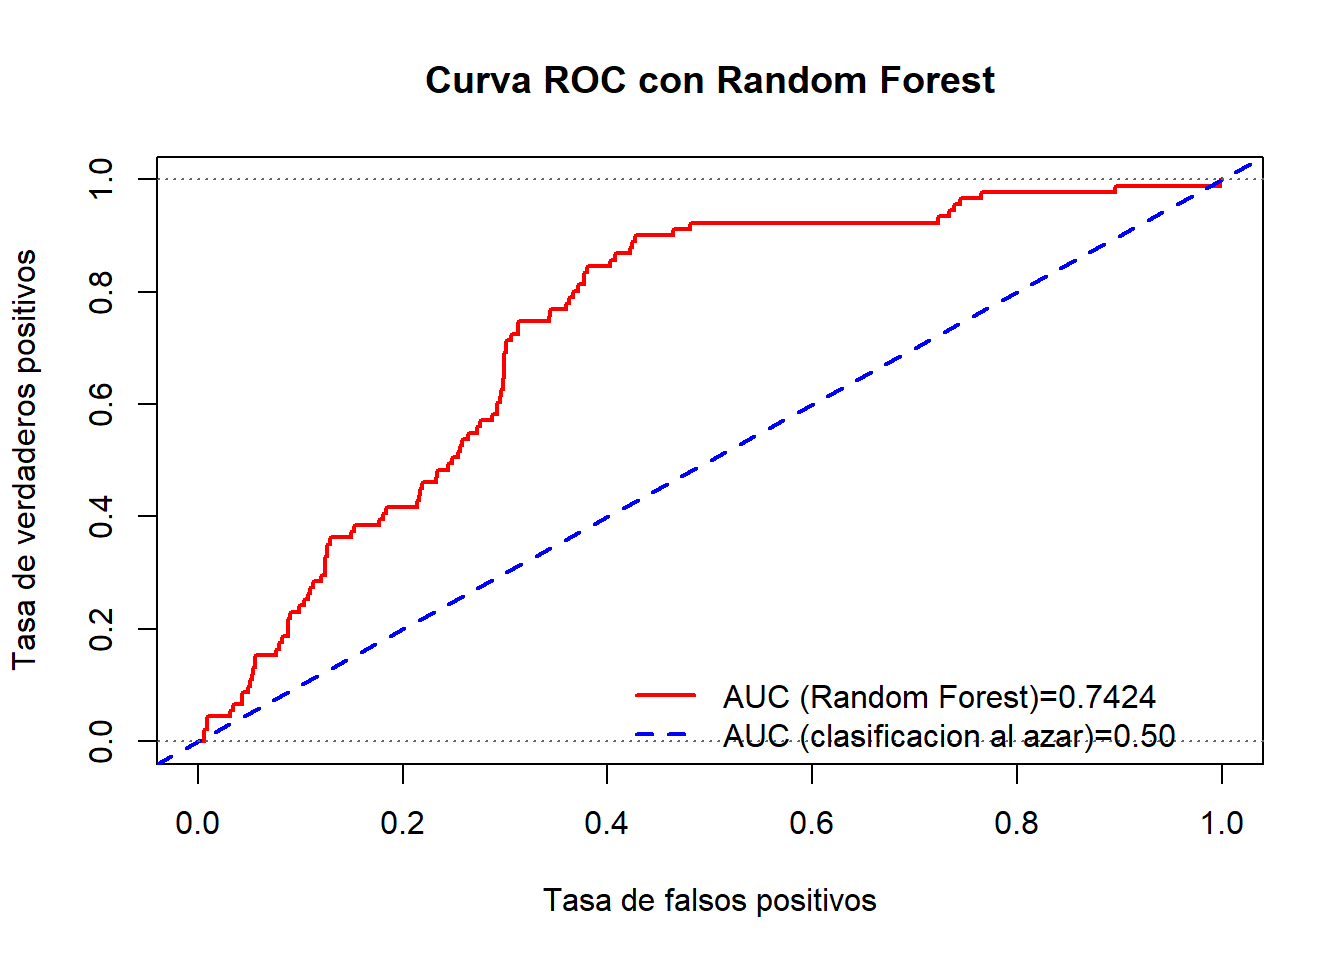
\includegraphics{02-Evaluation_files/figure-latex/unnamed-chunk-47-1.pdf}

\begin{itemize}
\tightlist
\item
  Se realizar el mismo gráfico de la curva ROC utilizando la librería \texttt{ggplot2}. Para ello guardamos los datos en un \texttt{data.frame}
\end{itemize}

\begin{Shaded}
\begin{Highlighting}[]
\KeywordTok{library}\NormalTok{(}\StringTok{"ggplot2"}\NormalTok{)}
\NormalTok{df.perf <-}\StringTok{ }\KeywordTok{data.frame}\NormalTok{(}\DataTypeTok{x=}\NormalTok{rf1.perf}\OperatorTok{@}\NormalTok{x.values[[}\DecValTok{1}\NormalTok{]],}\DataTypeTok{y=}\NormalTok{rf1.perf}\OperatorTok{@}\NormalTok{y.values[[}\DecValTok{1}\NormalTok{]])}
\end{Highlighting}
\end{Shaded}

\begin{itemize}
\tightlist
\item
  Construcción del objeto gráfico con \texttt{ggplot2}
\end{itemize}

\begin{Shaded}
\begin{Highlighting}[]
\CommentTok{#win.graph()}
\NormalTok{p <-}\StringTok{ }\KeywordTok{ggplot}\NormalTok{(df.perf,}\KeywordTok{aes}\NormalTok{(}\DataTypeTok{x=}\NormalTok{x,}\DataTypeTok{y=}\NormalTok{y)) }\OperatorTok{+}\StringTok{ }\KeywordTok{geom_path}\NormalTok{(}\DataTypeTok{size=}\DecValTok{1}\NormalTok{, }\DataTypeTok{colour=}\StringTok{"red"}\NormalTok{)}
\NormalTok{p <-}\StringTok{ }\NormalTok{p }\OperatorTok{+}\StringTok{ }\KeywordTok{ggtitle}\NormalTok{(}\StringTok{"Curva ROC modelo Random Forest"}\NormalTok{)}
\NormalTok{p <-}\StringTok{ }\NormalTok{p }\OperatorTok{+}\StringTok{ }\KeywordTok{theme_update}\NormalTok{(}\DataTypeTok{plot.title =} \KeywordTok{element_text}\NormalTok{(}\DataTypeTok{hjust =} \FloatTok{0.5}\NormalTok{))}
\NormalTok{p <-}\StringTok{ }\NormalTok{p }\OperatorTok{+}\StringTok{ }\KeywordTok{geom_segment}\NormalTok{(}\KeywordTok{aes}\NormalTok{(}\DataTypeTok{x=}\DecValTok{0}\NormalTok{,}\DataTypeTok{y=}\DecValTok{0}\NormalTok{,}\DataTypeTok{xend=}\DecValTok{1}\NormalTok{,}\DataTypeTok{yend=}\DecValTok{1}\NormalTok{),}\DataTypeTok{colour=}\StringTok{"blue"}\NormalTok{,}\DataTypeTok{linetype=} \DecValTok{2}\NormalTok{)}
\NormalTok{p <-}\StringTok{ }\NormalTok{p }\OperatorTok{+}\StringTok{ }\KeywordTok{geom_text}\NormalTok{(}\KeywordTok{aes}\NormalTok{(}\DataTypeTok{x=}\FloatTok{0.75}\NormalTok{ , }\DataTypeTok{y=}\FloatTok{0.3}\NormalTok{ , }\DataTypeTok{label=}\KeywordTok{paste}\NormalTok{(}\DataTypeTok{sep =}\StringTok{""}\NormalTok{,}\StringTok{"AUC (Random Forest) ) = "}\NormalTok{,}\KeywordTok{round}\NormalTok{(rf1.auc1,}\DecValTok{4}\NormalTok{) )),}\DataTypeTok{colour=}\StringTok{"black"}\NormalTok{,}\DataTypeTok{size=}\DecValTok{4}\NormalTok{)}
\NormalTok{p <-}\StringTok{ }\NormalTok{p }\OperatorTok{+}\StringTok{ }\KeywordTok{geom_text}\NormalTok{(}\KeywordTok{aes}\NormalTok{(}\DataTypeTok{x=}\FloatTok{0.75}\NormalTok{ , }\DataTypeTok{y=}\FloatTok{0.25}\NormalTok{ , }\DataTypeTok{label=}\KeywordTok{paste}\NormalTok{(}\DataTypeTok{sep =}\StringTok{""}\NormalTok{,}\StringTok{"AUC (Coin toss) = "}\NormalTok{,}\KeywordTok{round}\NormalTok{(}\FloatTok{0.50}\NormalTok{,}\DecValTok{4}\NormalTok{) )),}\DataTypeTok{colour=}\StringTok{"black"}\NormalTok{,}\DataTypeTok{size=}\DecValTok{4}\NormalTok{)}
\NormalTok{p <-}\StringTok{ }\NormalTok{p }\OperatorTok{+}\StringTok{ }\KeywordTok{scale_x_continuous}\NormalTok{(}\DataTypeTok{name=} \StringTok{"Tasa de falsos positivos"}\NormalTok{)}
\NormalTok{p <-}\StringTok{ }\NormalTok{p }\OperatorTok{+}\StringTok{ }\KeywordTok{scale_y_continuous}\NormalTok{(}\DataTypeTok{name=} \StringTok{"Tasa de verdaderos positivos"}\NormalTok{)}
\NormalTok{p <-}\StringTok{ }\NormalTok{p }\OperatorTok{+}\StringTok{ }\KeywordTok{theme}\NormalTok{(}
  \DataTypeTok{plot.title   =} \KeywordTok{element_text}\NormalTok{(}\DataTypeTok{size =} \DecValTok{2}\NormalTok{),}
  \DataTypeTok{axis.text.x  =} \KeywordTok{element_text}\NormalTok{(}\DataTypeTok{size =} \DecValTok{10}\NormalTok{),}
  \DataTypeTok{axis.text.y  =} \KeywordTok{element_text}\NormalTok{(}\DataTypeTok{size =} \DecValTok{10}\NormalTok{),}
  \DataTypeTok{axis.title.x =} \KeywordTok{element_text}\NormalTok{(}\DataTypeTok{size =} \DecValTok{12}\NormalTok{,}\DataTypeTok{face =} \StringTok{"italic"}\NormalTok{),}
  \DataTypeTok{axis.title.y =} \KeywordTok{element_text}\NormalTok{(}\DataTypeTok{size =} \DecValTok{12}\NormalTok{,}\DataTypeTok{face =} \StringTok{"italic"}\NormalTok{,}\DataTypeTok{angle=}\DecValTok{90}\NormalTok{),}
  \DataTypeTok{legend.title     =} \KeywordTok{element_blank}\NormalTok{(), }
  \DataTypeTok{panel.background =} \KeywordTok{element_rect}\NormalTok{(}\DataTypeTok{fill =} \StringTok{"grey"}\NormalTok{),}
  \DataTypeTok{panel.grid.minor =} \KeywordTok{element_blank}\NormalTok{(), }
  \DataTypeTok{panel.grid.major =} \KeywordTok{element_line}\NormalTok{(}\DataTypeTok{colour=}\StringTok{'white'}\NormalTok{),}
  \DataTypeTok{plot.background  =} \KeywordTok{element_blank}\NormalTok{()}
\NormalTok{)}

\NormalTok{p}
\end{Highlighting}
\end{Shaded}

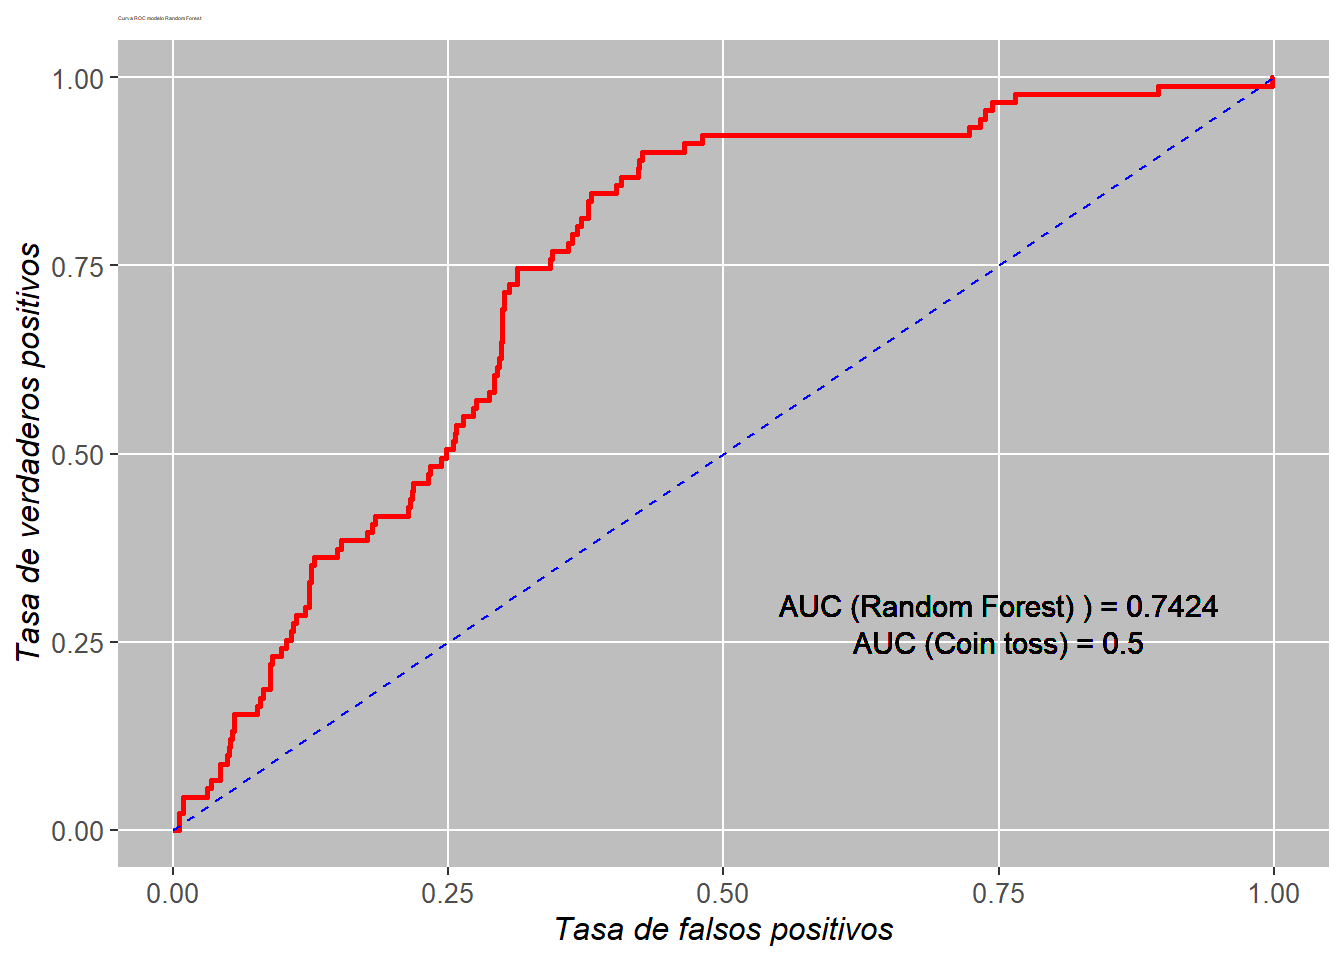
\includegraphics{02-Evaluation_files/figure-latex/unnamed-chunk-49-1.pdf}

\begin{quote}
Métricas de evaluación del poder predictivo
\end{quote}

\begin{itemize}
\tightlist
\item
  Calculamos la predicción en el \emph{test} y evaluamos el poder de clasificación del modelo
\end{itemize}

\begin{Shaded}
\begin{Highlighting}[]
\NormalTok{rf1.pred_test     <-}\StringTok{ }\KeywordTok{as.data.frame}\NormalTok{(}\KeywordTok{predict}\NormalTok{( rf1, }\DataTypeTok{newdata =}\NormalTok{ dt_test))}
\NormalTok{dt_test}\OperatorTok{$}\NormalTok{pred_rf1  <-}\StringTok{ }\NormalTok{rf1.pred_test}\OperatorTok{$}\StringTok{`}\DataTypeTok{predict(rf1, newdata = dt_test)}\StringTok{`} 
\end{Highlighting}
\end{Shaded}

\begin{Shaded}
\begin{Highlighting}[]
\KeywordTok{head}\NormalTok{(dt_test,}\DecValTok{3}\NormalTok{)}
\end{Highlighting}
\end{Shaded}

\begin{verbatim}
##    ATTORNEY CLMSEX MARITAL CLMINSUR SEATBELT CLMAGE   LOSS Y  pred_rf1
## 6         1      2       1        2        1     35  0.309 0 0.2279703
## 12        1      1       1        2        1     42 29.620 1 0.2159590
## 18        1      1       1        2        1     58  0.758 0 0.2047155
\end{verbatim}

\begin{Shaded}
\begin{Highlighting}[]
\KeywordTok{tail}\NormalTok{(dt_test,}\DecValTok{3}\NormalTok{)}
\end{Highlighting}
\end{Shaded}

\begin{verbatim}
##      ATTORNEY CLMSEX MARITAL CLMINSUR SEATBELT CLMAGE  LOSS Y    pred_rf1
## 1336        2      1       2        2        1     NA 0.576 0          NA
## 1337        1      2       1        2        1     46 3.705 0 0.349066396
## 1339        1      2       2        1        1     18 3.277 0 0.004032191
\end{verbatim}

\begin{Shaded}
\begin{Highlighting}[]
\KeywordTok{summary}\NormalTok{(dt_test)}
\end{Highlighting}
\end{Shaded}

\begin{verbatim}
##  ATTORNEY  CLMSEX    MARITAL    CLMINSUR   SEATBELT       CLMAGE     
##  1:214    1   :180   1   :185   1   : 43   1   :385   Min.   : 0.00  
##  2:188    2   :219   2   :195   2   :346   2   :  5   1st Qu.:19.00  
##           NA's:  3   3   :  5   NA's: 13   NA's: 12   Median :29.00  
##                      4   : 10                         Mean   :31.31  
##                      NA's:  7                         3rd Qu.:42.00  
##                                                       Max.   :78.00  
##                                                       NA's   :55     
##       LOSS                 Y             pred_rf1      
##  Min.   :   0.0050   Min.   :0.0000   Min.   :0.00005  
##  1st Qu.:   0.5175   1st Qu.:0.0000   1st Qu.:0.00797  
##  Median :   2.1645   Median :0.0000   Median :0.03794  
##  Mean   :   7.0917   Mean   :0.1144   Mean   :0.12531  
##  3rd Qu.:   3.7782   3rd Qu.:0.0000   3rd Qu.:0.21666  
##  Max.   :1067.6970   Max.   :1.0000   Max.   :0.75036  
##                                       NA's   :70
\end{verbatim}

\begin{itemize}
\tightlist
\item
  Con el \emph{test} creamos un objeto de tipo `prediction' y calculamos la curva ROC
\end{itemize}

\begin{Shaded}
\begin{Highlighting}[]
\NormalTok{dt_test.pred  <-}\StringTok{ }\KeywordTok{prediction}\NormalTok{(}\KeywordTok{as.numeric}\NormalTok{(rf1.pred_test}\OperatorTok{$}\StringTok{`}\DataTypeTok{predict(rf1, newdata = dt_test)}\StringTok{`}\NormalTok{),dt_test}\OperatorTok{$}\NormalTok{Y) }
\NormalTok{dt_test.perf  <-}\StringTok{ }\KeywordTok{performance}\NormalTok{(dt_test.pred,}\StringTok{"tpr"}\NormalTok{,}\StringTok{"fpr"}\NormalTok{) }
\end{Highlighting}
\end{Shaded}

\begin{itemize}
\tightlist
\item
  Evaluación del poder de clasificación del modelo RF1 vía curva ROC
\end{itemize}

\begin{Shaded}
\begin{Highlighting}[]
\NormalTok{rf1.test.auc <-}\StringTok{ }\KeywordTok{performance}\NormalTok{(dt_test.pred ,}\StringTok{"auc"}\NormalTok{)}\OperatorTok{@}\NormalTok{y.values[[}\DecValTok{1}\NormalTok{]]}
\end{Highlighting}
\end{Shaded}

\begin{itemize}
\tightlist
\item
  Gráfico de la curva ROC para el \emph{test}
\end{itemize}

\begin{Shaded}
\begin{Highlighting}[]
\CommentTok{#win.graph()}
\KeywordTok{plot}\NormalTok{( dt_test.perf , }\DataTypeTok{col=}\StringTok{'red'}\NormalTok{ , }\DataTypeTok{lwd=}\DecValTok{2}\NormalTok{, }\DataTypeTok{type=}\StringTok{"l"}\NormalTok{ , }\DataTypeTok{main=}\StringTok{"Curva ROC modelo RF - test"}\NormalTok{,}\DataTypeTok{xlab=}\StringTok{"Tasa de falsos positivos"}\NormalTok{, }\DataTypeTok{ylab=}\StringTok{"Tasa de verdaderos positivos"}\NormalTok{)}
\KeywordTok{abline}\NormalTok{( }\DecValTok{0}\NormalTok{ , }\DecValTok{1}\NormalTok{  , }\DataTypeTok{col=}\StringTok{"blue"}\NormalTok{ , }\DataTypeTok{lwd=}\DecValTok{2}\NormalTok{, }\DataTypeTok{lty=}\DecValTok{2}\NormalTok{)}
\KeywordTok{abline}\NormalTok{( }\DecValTok{0}\NormalTok{ , }\DecValTok{0}\NormalTok{ , }\DecValTok{1}\NormalTok{ , }\DataTypeTok{col=}\StringTok{"gray40"}\NormalTok{   , }\DataTypeTok{lty=}\DecValTok{3}\NormalTok{)}
\KeywordTok{legend}\NormalTok{( }\FloatTok{0.4}\NormalTok{, }\FloatTok{0.2}\NormalTok{ , }\KeywordTok{c}\NormalTok{(}\KeywordTok{paste0}\NormalTok{(}\StringTok{"AUC (Random Forest)="}\NormalTok{,}\KeywordTok{round}\NormalTok{(rf1.test.auc,}\DecValTok{4}\NormalTok{)),}\StringTok{"AUC (Coin toss)=0.50"}\NormalTok{) ,}\DataTypeTok{lty=}\KeywordTok{c}\NormalTok{(}\DecValTok{1}\NormalTok{,}\DecValTok{2}\NormalTok{), }\DataTypeTok{lwd=}\KeywordTok{c}\NormalTok{(}\DecValTok{2}\NormalTok{,}\DecValTok{2}\NormalTok{) ,}\DataTypeTok{col=}\KeywordTok{c}\NormalTok{(}\StringTok{"red"}\NormalTok{,}\StringTok{"blue"}\NormalTok{), }\DataTypeTok{bty=}\StringTok{"n"}\NormalTok{)}
\end{Highlighting}
\end{Shaded}

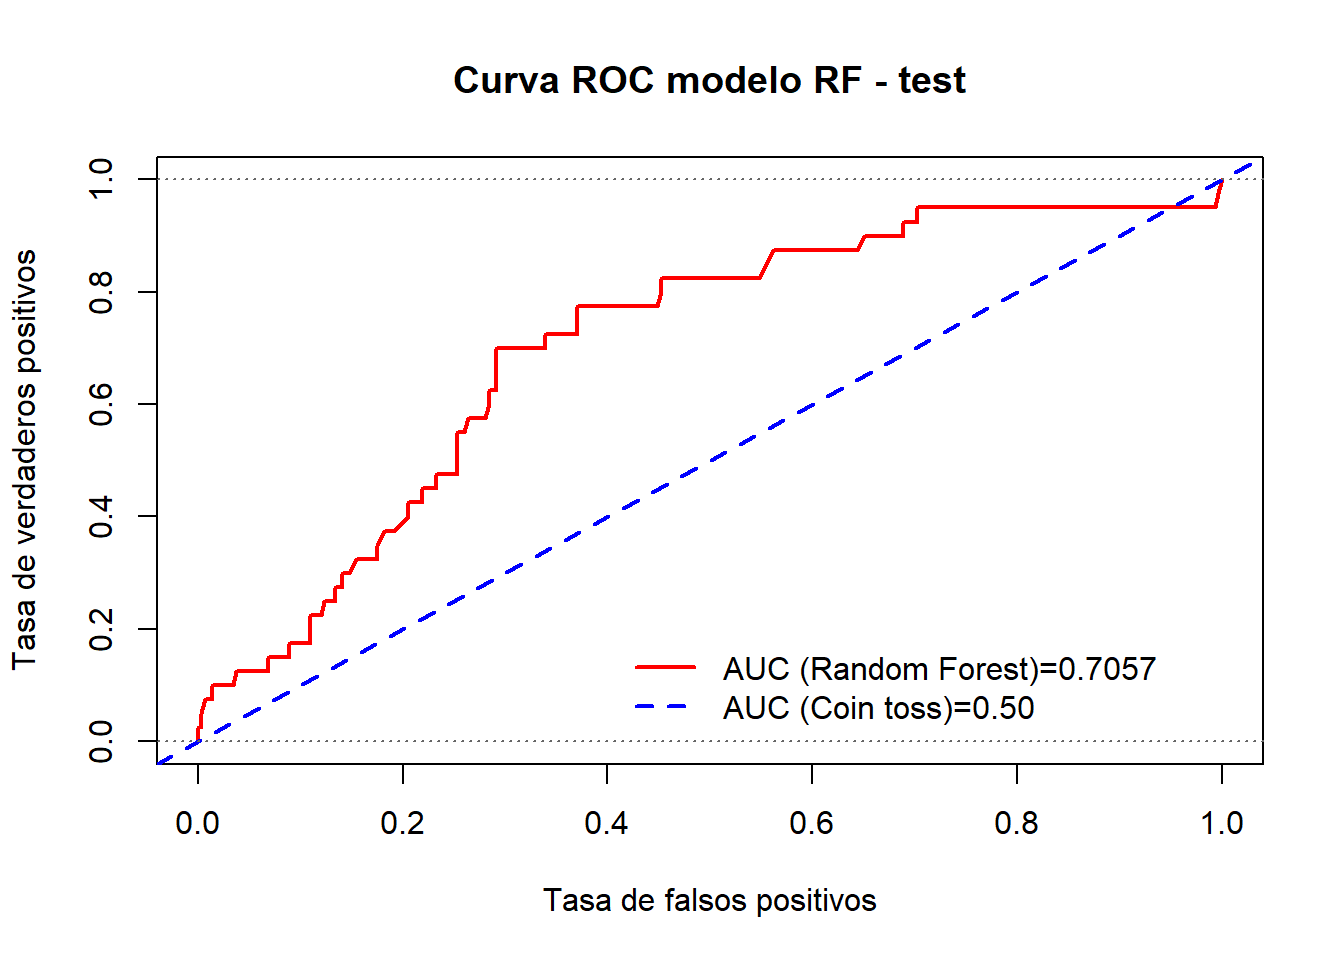
\includegraphics{02-Evaluation_files/figure-latex/unnamed-chunk-54-1.pdf}

\begin{quote}
Métrica de error del clasificador RF:
\end{quote}

\begin{itemize}
\tightlist
\item
  Error tipo I (\(\alpha\)): 22.50\%, indica el error que se comete clasificando una pérdida `severa' como `no severa'
\item
  Error tipo II (\(\beta\)): 43.15\%, indica el error que se comete clasificando una pérdida `no severa' como `severa'
\item
  \% mala clasificación (\(%mc
  \)) : 40.66\%, indica el \% de veces que el modelo clasifica incorrectamente las pérdidas
\item
  Accuracy = \(100 - %
  \): 59.34\%, indica el \% de veces que el modelo acierta clasificando las pérdidas
\item
  Area bajo la curva ROC \(AUC\): 0.6988, medida global del poder de clasificación del modelo
\item
  Finalmente calculamos la curva ROC junto con la métrica AUC
\end{itemize}

\begin{quote}
Resumiendo:
\end{quote}

Una función útil para obtener rápidamente el análisis de un clasificador binario es la siguiente:

\begin{Shaded}
\begin{Highlighting}[]
\NormalTok{metricBinaryClass =}\StringTok{ }\ControlFlowTok{function}\NormalTok{( fitted.model , dataset , }\DataTypeTok{cutpoint=}\OtherTok{NULL}\NormalTok{ , }\DataTypeTok{roc.graph=}\OtherTok{TRUE}\NormalTok{)\{}
  
  \CommentTok{# fitted.model : The Binary Classification model that is under evaluation. If provided, dataset contains all variables in the fitted model (target and predictors).}
  \CommentTok{# dataset      : If fitted.model is not provided, dataset should has only two columns, predictions and labels.}
  \CommentTok{# cuttpoint    : potimal cutoff or cutpoint to be used to split continuous predictions into two response categories of target variable}
  \CommentTok{# roc.graph    : If true, ROC curve graph for the model is shown }
  
  \CommentTok{#install.packages("binaryLogic")}
  \KeywordTok{library}\NormalTok{(binaryLogic)}
  
  \ControlFlowTok{if}\NormalTok{( }\KeywordTok{missing}\NormalTok{(fitted.model) }\OperatorTok{|}\StringTok{ }\KeywordTok{is.null}\NormalTok{(fitted.model) )\{}
    
\NormalTok{    tabl  <-}\StringTok{ }\KeywordTok{as.data.frame}\NormalTok{(dataset)}
\NormalTok{  \} }
  
  \ControlFlowTok{else}\NormalTok{ \{}
    \ControlFlowTok{if}\NormalTok{( }\KeywordTok{class}\NormalTok{(fitted.model)[}\DecValTok{1}\NormalTok{] }\OperatorTok\StringTok{ }\KeywordTok{c}\NormalTok{(}\StringTok{'glm'}\NormalTok{,}\StringTok{'lm'}\NormalTok{,}\StringTok{'randomForest.formula'}\NormalTok{,}\StringTok{'randomForest'}\NormalTok{) )\{}
\NormalTok{      tabl.pred <-}\StringTok{ }\KeywordTok{as.data.frame}\NormalTok{(}\KeywordTok{predict}\NormalTok{( fitted.model, }\DataTypeTok{newdata =}\NormalTok{ dataset ))}
\NormalTok{      tabl <-}\StringTok{ }\KeywordTok{as.data.frame}\NormalTok{(}\KeywordTok{cbind}\NormalTok{(tabl.pred[[}\DecValTok{1}\NormalTok{]], dataset[,}\StringTok{'Y'}\NormalTok{] )) }
\NormalTok{      tabl <-}\StringTok{ }\NormalTok{tabl[}\OperatorTok{!}\KeywordTok{is.na}\NormalTok{(tabl[[}\DecValTok{1}\NormalTok{]]),]}
\NormalTok{    \}}
    \ControlFlowTok{if}\NormalTok{( }\KeywordTok{class}\NormalTok{(fitted.model)[}\DecValTok{1}\NormalTok{] }\OperatorTok\StringTok{ }\KeywordTok{c}\NormalTok{(}\StringTok{"gbm"}\NormalTok{) )\{}
\NormalTok{      tabl.pred <-}\StringTok{ }\KeywordTok{as.data.frame}\NormalTok{(}\KeywordTok{predict.gbm}\NormalTok{( fitted.model , }\DataTypeTok{newdata =}\NormalTok{ dataset , }\DataTypeTok{n.trees =} \DecValTok{5000}\NormalTok{ , }\DataTypeTok{type=}\StringTok{"response"}\NormalTok{ ))}
\NormalTok{      tabl <-}\StringTok{ }\KeywordTok{as.data.frame}\NormalTok{(}\KeywordTok{cbind}\NormalTok{(tabl.pred[[}\DecValTok{1}\NormalTok{]], dataset[,}\StringTok{'Y'}\NormalTok{] )) }
\NormalTok{      tabl <-}\StringTok{ }\NormalTok{tabl[}\OperatorTok{!}\KeywordTok{is.na}\NormalTok{(tabl[[}\DecValTok{1}\NormalTok{]]),]}
\NormalTok{    \}}
    \ControlFlowTok{if}\NormalTok{( }\KeywordTok{class}\NormalTok{(fitted.model)[}\DecValTok{1}\NormalTok{] }\OperatorTok\StringTok{ }\KeywordTok{c}\NormalTok{(}\StringTok{'svm.formula'}\NormalTok{,}\StringTok{'svm'}\NormalTok{) )\{}
\NormalTok{      tabl.pred <-}\StringTok{ }\KeywordTok{as.data.frame}\NormalTok{(}\KeywordTok{predict}\NormalTok{( fitted.model, }\DataTypeTok{newdata =}\NormalTok{ dataset ))}
\NormalTok{      ids_NAs <-}\StringTok{ }\KeywordTok{na.index}\NormalTok{(dataset)}
\NormalTok{      tabl <-}\StringTok{ }\KeywordTok{as.data.frame}\NormalTok{( }\KeywordTok{cbind}\NormalTok{(tabl.pred[[}\DecValTok{1}\NormalTok{]], dataset[}\OperatorTok{-}\NormalTok{ids_NAs,}\StringTok{'Y'}\NormalTok{]) ) }
\NormalTok{      tabl <-}\StringTok{ }\NormalTok{tabl[}\OperatorTok{!}\KeywordTok{is.na}\NormalTok{(tabl[[}\DecValTok{1}\NormalTok{]]),]}
\NormalTok{    \}}
\NormalTok{  \}}
  \KeywordTok{colnames}\NormalTok{(tabl) <-}\StringTok{ }\KeywordTok{c}\NormalTok{(}\StringTok{'predicted'}\NormalTok{,}\StringTok{'actual'}\NormalTok{)}
  
  \CommentTok{# ROCR objects}
  \KeywordTok{require}\NormalTok{(ROCR)}
\NormalTok{  obj.pred <-}\StringTok{ }\KeywordTok{prediction}\NormalTok{(tabl}\OperatorTok{$}\NormalTok{predicted,tabl}\OperatorTok{$}\NormalTok{actual)}
\NormalTok{  obj.perf <-}\StringTok{ }\KeywordTok{performance}\NormalTok{(obj.pred,}\StringTok{"tpr"}\NormalTok{,}\StringTok{"fpr"}\NormalTok{)}
\NormalTok{  obj.auc  <-}\StringTok{ }\KeywordTok{performance}\NormalTok{(obj.pred,}\StringTok{"auc"}\NormalTok{)}\OperatorTok{@}\NormalTok{y.values[[}\DecValTok{1}\NormalTok{]]}
  \CommentTok{# For ROC curve:}
\NormalTok{  obj.perf}\OperatorTok{@}\NormalTok{alpha.values[[}\DecValTok{1}\NormalTok{]][obj.perf}\OperatorTok{@}\NormalTok{alpha.values[[}\DecValTok{1}\NormalTok{]]}\OperatorTok{==}\OtherTok{Inf}\NormalTok{] <-}\StringTok{ }\KeywordTok{max}\NormalTok{(obj.perf}\OperatorTok{@}\NormalTok{alpha.values[[}\DecValTok{1}\NormalTok{]][obj.perf}\OperatorTok{@}\NormalTok{alpha.values[[}\DecValTok{1}\NormalTok{]]}\OperatorTok{!=}\OtherTok{Inf}\NormalTok{])}
  \CommentTok{# KS criteria}
\NormalTok{  KS.matrix=}\StringTok{ }\KeywordTok{cbind}\NormalTok{(}\KeywordTok{abs}\NormalTok{(obj.perf}\OperatorTok{@}\NormalTok{y.values[[}\DecValTok{1}\NormalTok{]]}\OperatorTok{-}\NormalTok{obj.perf}\OperatorTok{@}\NormalTok{x.values[[}\DecValTok{1}\NormalTok{]]), obj.perf}\OperatorTok{@}\NormalTok{alpha.values[[}\DecValTok{1}\NormalTok{]])}
  \CommentTok{# KS cutoff}
  \CommentTok{# colnames(KS.matrix) <- c("KS-distance","cut-point")}
\NormalTok{  ind.ks  <-}\StringTok{ }\KeywordTok{sort}\NormalTok{( KS.matrix[,}\DecValTok{1}\NormalTok{] , }\DataTypeTok{index.return=}\OtherTok{TRUE}\NormalTok{ )}\OperatorTok{$}\NormalTok{ix[}\KeywordTok{nrow}\NormalTok{(KS.matrix)] }
  
  \ControlFlowTok{if}\NormalTok{( }\KeywordTok{missing}\NormalTok{(cutpoint) }\OperatorTok{|}\StringTok{ }\KeywordTok{is.null}\NormalTok{(cutpoint) ) cutpoint <-}\StringTok{ }\NormalTok{KS.matrix[ind.ks,}\DecValTok{2}\NormalTok{]}
  
  \ControlFlowTok{if}\NormalTok{( }\OperatorTok{!}\NormalTok{(}\KeywordTok{is.binary}\NormalTok{(tabl)) )\{}
    
    \CommentTok{# Make predictions objs.}
    \CommentTok{# Binary metrics }
\NormalTok{    tp =}\StringTok{ }\KeywordTok{sum}\NormalTok{( tabl}\OperatorTok{$}\NormalTok{predicted  }\OperatorTok{>}\StringTok{  }\NormalTok{cutpoint }\OperatorTok{&}\StringTok{ }\NormalTok{tabl}\OperatorTok{$}\NormalTok{actual }\OperatorTok{>}\StringTok{  }\NormalTok{cutpoint)}
\NormalTok{    fp =}\StringTok{ }\KeywordTok{sum}\NormalTok{( tabl}\OperatorTok{$}\NormalTok{predicted  }\OperatorTok{>}\StringTok{  }\NormalTok{cutpoint }\OperatorTok{&}\StringTok{ }\NormalTok{tabl}\OperatorTok{$}\NormalTok{actual }\OperatorTok{<=}\StringTok{ }\NormalTok{cutpoint)}
\NormalTok{    tn =}\StringTok{ }\KeywordTok{sum}\NormalTok{( tabl}\OperatorTok{$}\NormalTok{predicted  }\OperatorTok{<=}\StringTok{ }\NormalTok{cutpoint }\OperatorTok{&}\StringTok{ }\NormalTok{tabl}\OperatorTok{$}\NormalTok{actual }\OperatorTok{<=}\StringTok{ }\NormalTok{cutpoint)}
\NormalTok{    fn =}\StringTok{ }\KeywordTok{sum}\NormalTok{( tabl}\OperatorTok{$}\NormalTok{predicted  }\OperatorTok{<=}\StringTok{ }\NormalTok{cutpoint }\OperatorTok{&}\StringTok{ }\NormalTok{tabl}\OperatorTok{$}\NormalTok{actual }\OperatorTok{>}\StringTok{  }\NormalTok{cutpoint) }
\NormalTok{    pos =}\StringTok{ }\NormalTok{tp}\OperatorTok{+}\NormalTok{fn}
\NormalTok{    neg =}\StringTok{ }\NormalTok{tn}\OperatorTok{+}\NormalTok{fp}
\NormalTok{    acc=}\StringTok{  }\DecValTok{100}\OperatorTok{*}\NormalTok{(tp}\OperatorTok{+}\NormalTok{tn)}\OperatorTok{/}\NormalTok{(pos}\OperatorTok{+}\NormalTok{neg)}
\NormalTok{    prec=}\StringTok{ }\DecValTok{100}\OperatorTok{*}\NormalTok{tp}\OperatorTok{/}\NormalTok{(tp}\OperatorTok{+}\NormalTok{fp)}
\NormalTok{    sens=}\StringTok{ }\DecValTok{100}\OperatorTok{*}\NormalTok{tp}\OperatorTok{/}\NormalTok{(tp}\OperatorTok{+}\NormalTok{fn) }\CommentTok{# = tpr = recall = 1 - error alpha}
\NormalTok{    spec=}\StringTok{ }\DecValTok{100}\OperatorTok{*}\NormalTok{tn}\OperatorTok{/}\NormalTok{(tn}\OperatorTok{+}\NormalTok{fp) }\CommentTok{# 1- error beta}
\NormalTok{    fpr =}\StringTok{ }\DecValTok{100}\OperatorTok{*}\NormalTok{fp}\OperatorTok{/}\NormalTok{neg  }\CommentTok{# error beta (tipo II) = 1 - spec}
\NormalTok{    fnr =}\StringTok{ }\DecValTok{100}\OperatorTok{*}\NormalTok{fn}\OperatorTok{/}\NormalTok{pos  }\CommentTok{# error alpha (tipo I) = 1- recall = 1- sens}
\NormalTok{  \}}
  
  \ControlFlowTok{if}\NormalTok{( }\KeywordTok{is.binary}\NormalTok{(tabl) )\{}
    
\NormalTok{    tp =}\StringTok{ }\KeywordTok{sum}\NormalTok{( tabl}\OperatorTok{$}\NormalTok{predicted  }\OperatorTok{==}\StringTok{ }\DecValTok{1} \OperatorTok{&}\StringTok{ }\NormalTok{tabl}\OperatorTok{$}\NormalTok{actual }\OperatorTok{==}\StringTok{ }\DecValTok{1}\NormalTok{)}
\NormalTok{    fp =}\StringTok{ }\KeywordTok{sum}\NormalTok{( tabl}\OperatorTok{$}\NormalTok{predicted  }\OperatorTok{==}\StringTok{ }\DecValTok{1} \OperatorTok{&}\StringTok{ }\NormalTok{tabl}\OperatorTok{$}\NormalTok{actual }\OperatorTok{==}\StringTok{ }\DecValTok{0}\NormalTok{)}
\NormalTok{    tn =}\StringTok{ }\KeywordTok{sum}\NormalTok{( tabl}\OperatorTok{$}\NormalTok{predicted  }\OperatorTok{==}\StringTok{ }\DecValTok{0} \OperatorTok{&}\StringTok{ }\NormalTok{tabl}\OperatorTok{$}\NormalTok{actual }\OperatorTok{==}\StringTok{ }\DecValTok{0}\NormalTok{)}
\NormalTok{    fn =}\StringTok{ }\KeywordTok{sum}\NormalTok{( tabl}\OperatorTok{$}\NormalTok{predicted  }\OperatorTok{==}\StringTok{ }\DecValTok{0} \OperatorTok{&}\StringTok{ }\NormalTok{tabl}\OperatorTok{$}\NormalTok{actual }\OperatorTok{==}\StringTok{ }\DecValTok{1}\NormalTok{) }
\NormalTok{    pos =}\StringTok{ }\NormalTok{tp}\OperatorTok{+}\NormalTok{fn}
\NormalTok{    neg =}\StringTok{ }\NormalTok{tn}\OperatorTok{+}\NormalTok{fp}
\NormalTok{    acc=}\StringTok{  }\DecValTok{100}\OperatorTok{*}\NormalTok{(tp}\OperatorTok{+}\NormalTok{tn)}\OperatorTok{/}\NormalTok{(pos}\OperatorTok{+}\NormalTok{neg)}
\NormalTok{    prec=}\StringTok{ }\DecValTok{100}\OperatorTok{*}\NormalTok{tp}\OperatorTok{/}\NormalTok{(tp}\OperatorTok{+}\NormalTok{fp)}
\NormalTok{    sens=}\StringTok{ }\DecValTok{100}\OperatorTok{*}\NormalTok{tp}\OperatorTok{/}\NormalTok{(tp}\OperatorTok{+}\NormalTok{fn) }\CommentTok{# = tpr = recall = 1 - error alpha}
\NormalTok{    spec=}\StringTok{ }\DecValTok{100}\OperatorTok{*}\NormalTok{tn}\OperatorTok{/}\NormalTok{(tn}\OperatorTok{+}\NormalTok{fp) }\CommentTok{# 1- error beta}
\NormalTok{    fpr =}\StringTok{ }\DecValTok{100}\OperatorTok{*}\NormalTok{fp}\OperatorTok{/}\NormalTok{neg  }\CommentTok{# error beta (tipo II) = 1 - spec}
\NormalTok{    fnr =}\StringTok{ }\DecValTok{100}\OperatorTok{*}\NormalTok{fn}\OperatorTok{/}\NormalTok{pos  }\CommentTok{# error alpha (tipo I) = 1- recall = 1- sens}
\NormalTok{  \}  }
  
  \ControlFlowTok{if}\NormalTok{(roc.graph}\OperatorTok{==}\OtherTok{TRUE}\NormalTok{)\{}
    \KeywordTok{win.graph}\NormalTok{()}
    \KeywordTok{plot}\NormalTok{( obj.perf  , }\DataTypeTok{col=}\StringTok{'red'}\NormalTok{ , }\DataTypeTok{lwd=}\DecValTok{2}\NormalTok{, }\DataTypeTok{type=}\StringTok{"l"}\NormalTok{,}\DataTypeTok{xlab=}\StringTok{"Tasa de falsos positivos"}\NormalTok{ , }\DataTypeTok{ylab=}\StringTok{"Tasa de verdaderos positivos"}\NormalTok{, }\DataTypeTok{main=}\StringTok{"Curva ROC modelo clasificación")}
\StringTok{    abline( 0.0 , 1.0 , col="}\NormalTok{blue}\StringTok{", lwd=2, lty=2)}
\StringTok{    abline( 0.0 , 0.0 , 1 , col="}\NormalTok{gray40}\StringTok{" , lty=3)}
\StringTok{    legend( 0.45, 0.2 , c(paste0("}\KeywordTok{AUC}\NormalTok{ (Model)=}\StringTok{",round(obj.auc,4)),"}\KeywordTok{AUC}\NormalTok{ (Rolling dice)=}\FloatTok{0.50}\StringTok{") ,lty=c(1,2), lwd=c(2,2) ,col=c("}\NormalTok{red}\StringTok{","}\NormalTok{blue}\StringTok{"), bty="}\NormalTok{n}\StringTok{")}
\StringTok{  \}}
\StringTok{  }
\StringTok{  list(ClassError.tI=round(fnr,2), ClassError.tII=round(fpr,2), Accuracy=round(acc,2),Sensitivity = round(sens,2) , Specificity= round(spec,2), auc= obj.auc , Fisher.F1=round(2*prec*sens/(prec+sens),4) )}
\StringTok{  }
\StringTok{\}}
\end{Highlighting}
\end{Shaded}

\begin{Shaded}
\begin{Highlighting}[]
 \KeywordTok{metricBinaryClass}\NormalTok{( }\DataTypeTok{fitted.model =}\NormalTok{ rf1 , }\DataTypeTok{dataset=}\NormalTok{ dt_test , }\DataTypeTok{cutpoint=}\NormalTok{rf1.KScutoff , }\DataTypeTok{roc.graph=}\OtherTok{TRUE}\NormalTok{)}
\end{Highlighting}
\end{Shaded}

\begin{verbatim}
## $ClassError.tI
## [1] 22.5
## 
## $ClassError.tII
## [1] 43.49
## 
## $Accuracy
## [1] 59.04
## 
## $Sensitivity
## [1] 77.5
## 
## $Specificity
## [1] 56.51
## 
## $auc
## [1] 0.7056507
## 
## $Fisher.F1
## [1] 31.3131
\end{verbatim}

\hypertarget{regresion}{%
\subsection{Regresión}\label{regresion}}

Vamos a construir un modelo para prever las pérdidas.

\begin{quote}
Modelo con \emph{Random Forest} en \emph{train}
\end{quote}

\begin{Shaded}
\begin{Highlighting}[]
\NormalTok{fmla.rf2 <-}\StringTok{ }\KeywordTok{as.formula}\NormalTok{(}\KeywordTok{paste0}\NormalTok{(}\StringTok{'LOSS'}\NormalTok{,}\StringTok{'~'}\NormalTok{,}\KeywordTok{paste0}\NormalTok{(}\KeywordTok{colnames}\NormalTok{(df_autobi[,}\OperatorTok{-}\KeywordTok{c}\NormalTok{(}\DecValTok{7}\NormalTok{,}\DecValTok{8}\NormalTok{)]),}\DataTypeTok{collapse =} \StringTok{"+"}\NormalTok{),}\DataTypeTok{collapse =} \StringTok{''}\NormalTok{))}
\KeywordTok{set.seed}\NormalTok{(}\DecValTok{112233}\NormalTok{) }\CommentTok{#recomendado}

\NormalTok{rf2 <-}\StringTok{ }\KeywordTok{randomForest}\NormalTok{( fmla.rf2,}
                     \DataTypeTok{data =}\NormalTok{dt_train,}
                     \DataTypeTok{ntree =} \DecValTok{5000}\NormalTok{,}
                     \DataTypeTok{replace =}\OtherTok{TRUE}\NormalTok{,}
                     \DataTypeTok{mtry=}\DecValTok{4}\NormalTok{,}
                     \DataTypeTok{maxnodes =}\DecValTok{50}\NormalTok{,}
                     \DataTypeTok{importance =} \OtherTok{TRUE}\NormalTok{,}
                     \DataTypeTok{na.action=}\NormalTok{na.omit)}

\KeywordTok{summary}\NormalTok{(rf2)}
\end{Highlighting}
\end{Shaded}

\begin{verbatim}
##                 Length Class  Mode     
## call               9   -none- call     
## type               1   -none- character
## predicted        759   -none- numeric  
## mse             5000   -none- numeric  
## rsq             5000   -none- numeric  
## oob.times        759   -none- numeric  
## importance        12   -none- numeric  
## importanceSD       6   -none- numeric  
## localImportance    0   -none- NULL     
## proximity          0   -none- NULL     
## ntree              1   -none- numeric  
## mtry               1   -none- numeric  
## forest            11   -none- list     
## coefs              0   -none- NULL     
## y                759   -none- numeric  
## test               0   -none- NULL     
## inbag              0   -none- NULL     
## terms              3   terms  call     
## na.action        179   omit   numeric
\end{verbatim}

\begin{Shaded}
\begin{Highlighting}[]
\KeywordTok{str}\NormalTok{(rf2)}
\end{Highlighting}
\end{Shaded}

\begin{verbatim}
## List of 19
##  $ call           : language randomForest(formula = fmla.rf2, data = dt_train, ntree = 5000, replace = TRUE,      mtry = 4, maxnodes = 50, imp| __truncated__
##  $ type           : chr "regression"
##  $ predicted      : Named num [1:759] 2.407 0.676 37.029 1.73 4.229 ...
##   ..- attr(*, "names")= chr [1:759] "2" "3" "4" "5" ...
##   ..- attr(*, "na.action")= 'omit' Named int [1:179] 1 9 19 25 27 40 43 46 50 51 ...
##   .. ..- attr(*, "names")= chr [1:179] "1" "10" "24" "30" ...
##  $ mse            : num [1:5000] 566 483 441 401 427 ...
##  $ rsq            : num [1:5000] -0.707 -0.457 -0.328 -0.208 -0.286 ...
##  $ oob.times      : int [1:759] 1820 1870 1853 1846 1856 1840 1820 1899 1880 1876 ...
##  $ importance     : num [1:6, 1:2] 17.313 0.136 -3.726 3.199 4.752 ...
##   ..- attr(*, "dimnames")=List of 2
##   .. ..$ : chr [1:6] "ATTORNEY" "CLMSEX" "MARITAL" "CLMINSUR" ...
##   .. ..$ : chr [1:2] "%IncMSE" "IncNodePurity"
##  $ importanceSD   : Named num [1:6] 1.215 1.018 1.116 0.38 0.743 ...
##   ..- attr(*, "names")= chr [1:6] "ATTORNEY" "CLMSEX" "MARITAL" "CLMINSUR" ...
##  $ localImportance: NULL
##  $ proximity      : NULL
##  $ ntree          : num 5000
##  $ mtry           : num 4
##  $ forest         :List of 11
##   ..$ ndbigtree    : int [1:5000] 99 99 99 99 99 99 99 99 99 99 ...
##   ..$ nodestatus   : int [1:99, 1:5000] -3 -3 -3 -3 -3 -3 -1 -3 -3 -3 ...
##   ..$ leftDaughter : int [1:99, 1:5000] 2 4 6 8 10 12 0 14 16 18 ...
##   ..$ rightDaughter: int [1:99, 1:5000] 3 5 7 9 11 13 0 15 17 19 ...
##   ..$ nodepred     : num [1:99, 1:5000] 4.96 4.6 23.76 7.19 1.9 ...
##   ..$ bestvar      : int [1:99, 1:5000] 5 1 6 3 6 3 0 6 2 3 ...
##   ..$ xbestsplit   : num [1:99, 1:5000] 1.5 1.5 37.5 3.5 20.5 1.5 0 25.5 1.5 1.5 ...
##   ..$ ncat         : Named int [1:6] 1 1 1 1 1 1
##   .. ..- attr(*, "names")= chr [1:6] "ATTORNEY" "CLMSEX" "MARITAL" "CLMINSUR" ...
##   ..$ nrnodes      : int 99
##   ..$ ntree        : num 5000
##   ..$ xlevels      :List of 6
##   .. ..$ ATTORNEY: num 0
##   .. ..$ CLMSEX  : num 0
##   .. ..$ MARITAL : num 0
##   .. ..$ CLMINSUR: num 0
##   .. ..$ SEATBELT: num 0
##   .. ..$ CLMAGE  : num 0
##  $ coefs          : NULL
##  $ y              : Named num [1:759] 10.892 0.33 11.037 0.138 3.538 ...
##   ..- attr(*, "na.action")= 'omit' Named int [1:179] 1 9 19 25 27 40 43 46 50 51 ...
##   .. ..- attr(*, "names")= chr [1:179] "1" "10" "24" "30" ...
##   ..- attr(*, "names")= chr [1:759] "2" "3" "4" "5" ...
##  $ test           : NULL
##  $ inbag          : NULL
##  $ terms          :Classes 'terms', 'formula'  language LOSS ~ ATTORNEY + CLMSEX + MARITAL + CLMINSUR + SEATBELT + CLMAGE
##   .. ..- attr(*, "variables")= language list(LOSS, ATTORNEY, CLMSEX, MARITAL, CLMINSUR, SEATBELT, CLMAGE)
##   .. ..- attr(*, "factors")= int [1:7, 1:6] 0 1 0 0 0 0 0 0 0 1 ...
##   .. .. ..- attr(*, "dimnames")=List of 2
##   .. .. .. ..$ : chr [1:7] "LOSS" "ATTORNEY" "CLMSEX" "MARITAL" ...
##   .. .. .. ..$ : chr [1:6] "ATTORNEY" "CLMSEX" "MARITAL" "CLMINSUR" ...
##   .. ..- attr(*, "term.labels")= chr [1:6] "ATTORNEY" "CLMSEX" "MARITAL" "CLMINSUR" ...
##   .. ..- attr(*, "order")= int [1:6] 1 1 1 1 1 1
##   .. ..- attr(*, "intercept")= num 0
##   .. ..- attr(*, "response")= int 1
##   .. ..- attr(*, ".Environment")=<environment: R_GlobalEnv> 
##   .. ..- attr(*, "predvars")= language list(LOSS, ATTORNEY, CLMSEX, MARITAL, CLMINSUR, SEATBELT, CLMAGE)
##   .. ..- attr(*, "dataClasses")= Named chr [1:7] "numeric" "ordered" "ordered" "ordered" ...
##   .. .. ..- attr(*, "names")= chr [1:7] "LOSS" "ATTORNEY" "CLMSEX" "MARITAL" ...
##  $ na.action      : 'omit' Named int [1:179] 1 9 19 25 27 40 43 46 50 51 ...
##   ..- attr(*, "names")= chr [1:179] "1" "10" "24" "30" ...
##  - attr(*, "class")= chr [1:2] "randomForest.formula" "randomForest"
\end{verbatim}

\begin{quote}
Importancia Relativa de las Variables \emph{Input}
\end{quote}

\begin{Shaded}
\begin{Highlighting}[]
\KeywordTok{varImpPlot}\NormalTok{(rf2,}\DataTypeTok{sort =}\NormalTok{ T,}\DataTypeTok{main=}\StringTok{"Variable Importance"}\NormalTok{)}
\end{Highlighting}
\end{Shaded}

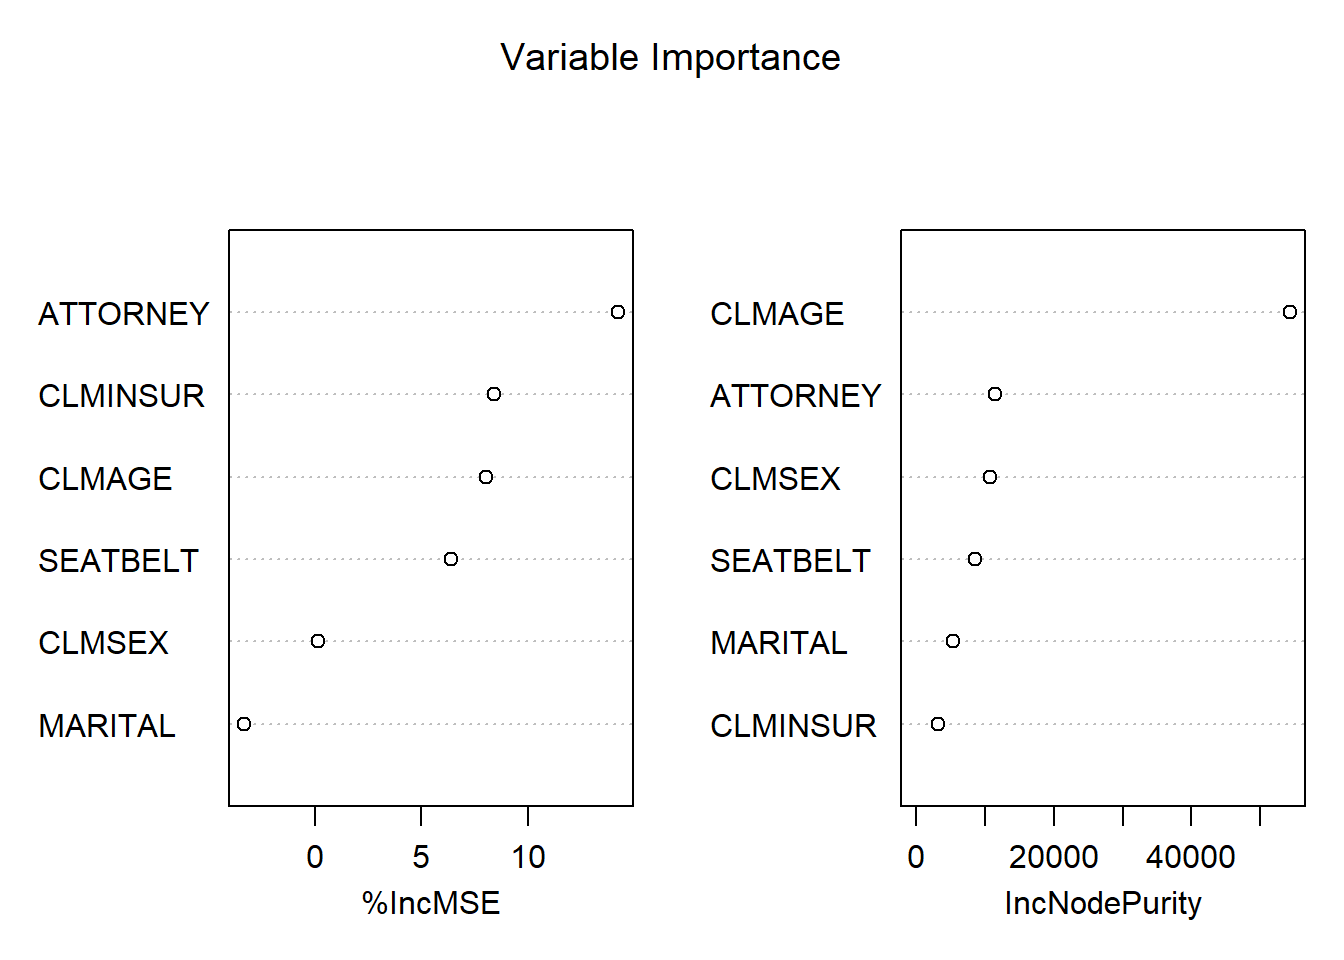
\includegraphics{02-Evaluation_files/figure-latex/unnamed-chunk-59-1.pdf}

\begin{quote}
Previsión en \emph{test}
\end{quote}

\begin{Shaded}
\begin{Highlighting}[]
\NormalTok{rf2.prediction <-}\StringTok{ }\KeywordTok{as.data.frame}\NormalTok{(}\KeywordTok{predict}\NormalTok{(rf2, }\DataTypeTok{newdata =}\NormalTok{ dt_test))}
\NormalTok{dt_test}\OperatorTok{$}\NormalTok{pred_rf2 <-}\StringTok{ }\NormalTok{rf2.prediction[[}\DecValTok{1}\NormalTok{]] }
\end{Highlighting}
\end{Shaded}

\begin{Shaded}
\begin{Highlighting}[]
\KeywordTok{head}\NormalTok{(dt_test, }\DecValTok{3}\NormalTok{)}
\end{Highlighting}
\end{Shaded}

\begin{verbatim}
##    ATTORNEY CLMSEX MARITAL CLMINSUR SEATBELT CLMAGE   LOSS Y  pred_rf1
## 6         1      2       1        2        1     35  0.309 0 0.2279703
## 12        1      1       1        2        1     42 29.620 1 0.2159590
## 18        1      1       1        2        1     58  0.758 0 0.2047155
##    pred_rf2
## 6  7.914295
## 12 8.539666
## 18 9.864992
\end{verbatim}

\begin{Shaded}
\begin{Highlighting}[]
\KeywordTok{tail}\NormalTok{(dt_test, }\DecValTok{3}\NormalTok{)}
\end{Highlighting}
\end{Shaded}

\begin{verbatim}
##      ATTORNEY CLMSEX MARITAL CLMINSUR SEATBELT CLMAGE  LOSS Y    pred_rf1
## 1336        2      1       2        2        1     NA 0.576 0          NA
## 1337        1      2       1        2        1     46 3.705 0 0.349066396
## 1339        1      2       2        1        1     18 3.277 0 0.004032191
##       pred_rf2
## 1336        NA
## 1337 36.877666
## 1339  3.963606
\end{verbatim}

\begin{Shaded}
\begin{Highlighting}[]
\KeywordTok{summary}\NormalTok{(dt_test, }\DecValTok{3}\NormalTok{)}
\end{Highlighting}
\end{Shaded}

\begin{verbatim}
##  ATTORNEY  CLMSEX       MARITAL    CLMINSUR   SEATBELT       CLMAGE     
##  1:214    1   :180   2      :195   1   : 43   1   :385   Min.   : 0.00  
##  2:188    2   :219   (Other):200   2   :346   2   :  5   1st Qu.:19.00  
##           NA's:  3   NA's   :  7   NA's: 13   NA's: 12   Median :29.00  
##                                                          Mean   :31.31  
##                                                          3rd Qu.:42.00  
##                                                          Max.   :78.00  
##                                                          NA's   :55     
##       LOSS                 Y             pred_rf1          pred_rf2     
##  Min.   :   0.0050   Min.   :0.0000   Min.   :0.00005   Min.   : 0.377  
##  1st Qu.:   0.5175   1st Qu.:0.0000   1st Qu.:0.00797   1st Qu.: 2.048  
##  Median :   2.1645   Median :0.0000   Median :0.03794   Median : 3.293  
##  Mean   :   7.0917   Mean   :0.1144   Mean   :0.12531   Mean   : 6.375  
##  3rd Qu.:   3.7782   3rd Qu.:0.0000   3rd Qu.:0.21666   3rd Qu.: 7.881  
##  Max.   :1067.6970   Max.   :1.0000   Max.   :0.75036   Max.   :56.904  
##                                       NA's   :70        NA's   :70
\end{verbatim}

\begin{quote}
Graficamos la distribución de los valores estimados en el \emph{train}
\end{quote}

\begin{Shaded}
\begin{Highlighting}[]
\KeywordTok{plot}\NormalTok{(}\KeywordTok{density}\NormalTok{(dt_test}\OperatorTok{$}\NormalTok{pred_rf2[}\OperatorTok{!}\KeywordTok{is.na}\NormalTok{(dt_test}\OperatorTok{$}\NormalTok{pred_rf2) }\OperatorTok{&}\StringTok{ }\NormalTok{dt_test}\OperatorTok{$}\NormalTok{pred_rf2 }\OperatorTok{<}\StringTok{ }\DecValTok{30}\NormalTok{]), }\DataTypeTok{ylim=} \KeywordTok{c}\NormalTok{(}\DecValTok{0}\NormalTok{,.}\DecValTok{25}\NormalTok{) , }\DataTypeTok{col=}\StringTok{"red"}\NormalTok{ , }\DataTypeTok{main=}\StringTok{""}\NormalTok{)}
\KeywordTok{lines}\NormalTok{(}\KeywordTok{density}\NormalTok{(dt_test}\OperatorTok{$}\NormalTok{LOSS[dt_test}\OperatorTok{$}\NormalTok{LOSS}\OperatorTok{<}\DecValTok{30}\NormalTok{]),}\DataTypeTok{col=}\StringTok{"blue"}\NormalTok{,}\DataTypeTok{lty=}\DecValTok{1}\NormalTok{)}
\end{Highlighting}
\end{Shaded}

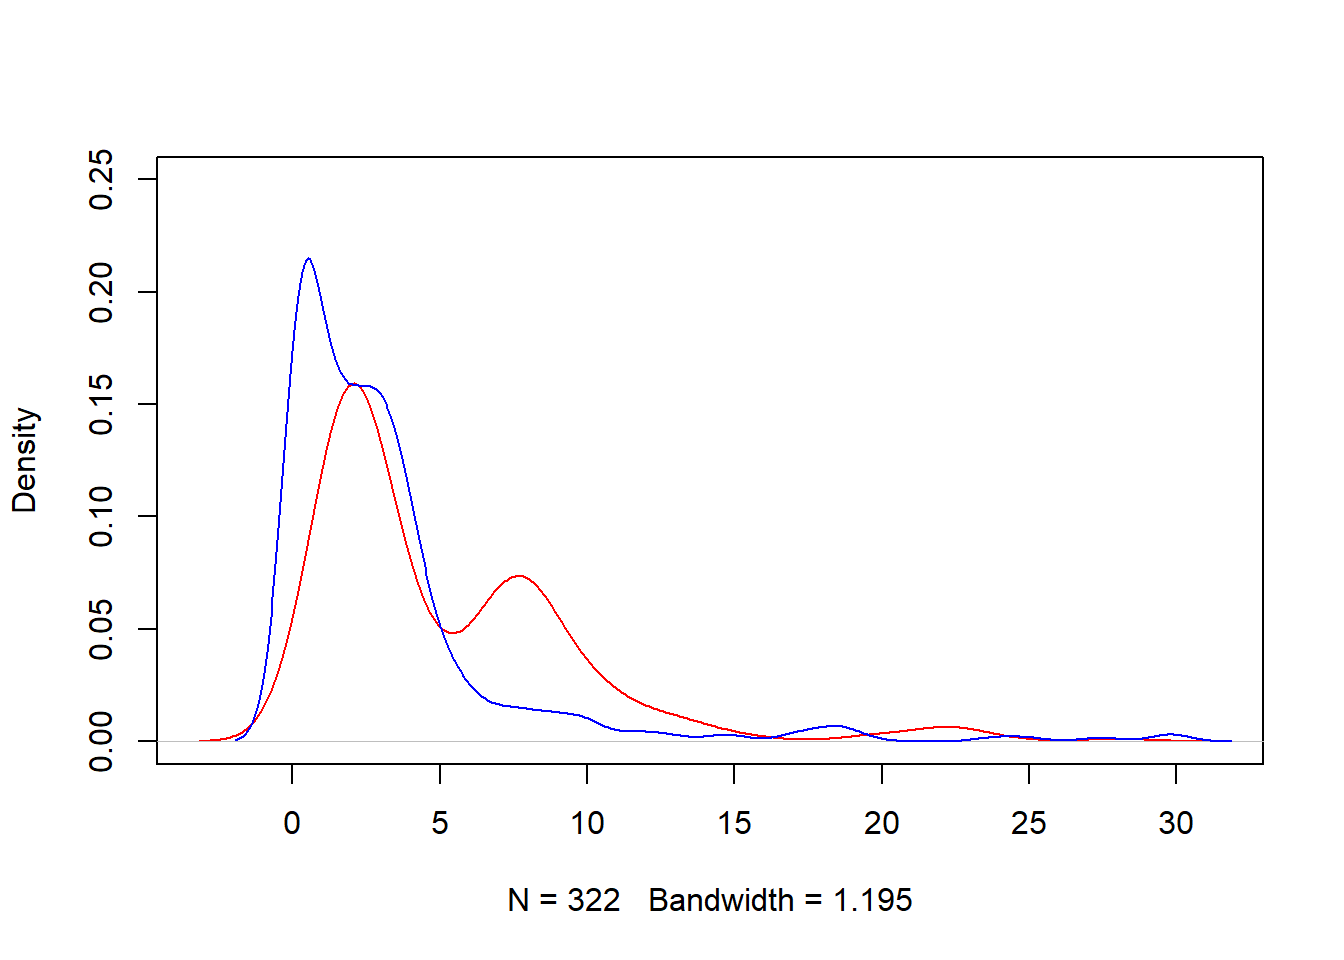
\includegraphics{02-Evaluation_files/figure-latex/unnamed-chunk-62-1.pdf}

\begin{Shaded}
\begin{Highlighting}[]
\NormalTok{modelchecktest1 <-}\StringTok{ }\KeywordTok{as.data.frame}\NormalTok{( }\KeywordTok{cbind}\NormalTok{(}\DataTypeTok{real=}\NormalTok{dt_test}\OperatorTok{$}\NormalTok{LOSS , }\DataTypeTok{predicted=}\NormalTok{dt_test}\OperatorTok{$}\NormalTok{pred_rf2) )}
\NormalTok{modelchecktest1[}\KeywordTok{is.na}\NormalTok{(modelchecktest1)] <-}\StringTok{ }\DecValTok{0}

\KeywordTok{summary}\NormalTok{(modelchecktest1)}
\end{Highlighting}
\end{Shaded}

\begin{verbatim}
##       real             predicted     
##  Min.   :   0.0050   Min.   : 0.000  
##  1st Qu.:   0.5175   1st Qu.: 1.310  
##  Median :   2.1645   Median : 2.422  
##  Mean   :   7.0917   Mean   : 5.265  
##  3rd Qu.:   3.7782   3rd Qu.: 7.469  
##  Max.   :1067.6970   Max.   :56.904
\end{verbatim}

\begin{quote}
Error de ajuste del modelo
\end{quote}

\begin{Shaded}
\begin{Highlighting}[]
\KeywordTok{plot}\NormalTok{(modelchecktest1, }\DataTypeTok{xlim=}\KeywordTok{c}\NormalTok{(}\DecValTok{0}\NormalTok{,}\DecValTok{100}\NormalTok{) , }\DataTypeTok{ylim=}\KeywordTok{c}\NormalTok{(}\DecValTok{0}\NormalTok{,}\DecValTok{100}\NormalTok{) ,  }\DataTypeTok{pch=}\StringTok{"."}\NormalTok{ , }\DataTypeTok{cex=}\FloatTok{1.5}\NormalTok{)}
\KeywordTok{segments}\NormalTok{( }\DecValTok{0}\NormalTok{, }\DecValTok{0}\NormalTok{ , }\DecValTok{100}\NormalTok{, }\DecValTok{100}\NormalTok{ , }\DataTypeTok{col=}\StringTok{"red"}\NormalTok{)}
\end{Highlighting}
\end{Shaded}

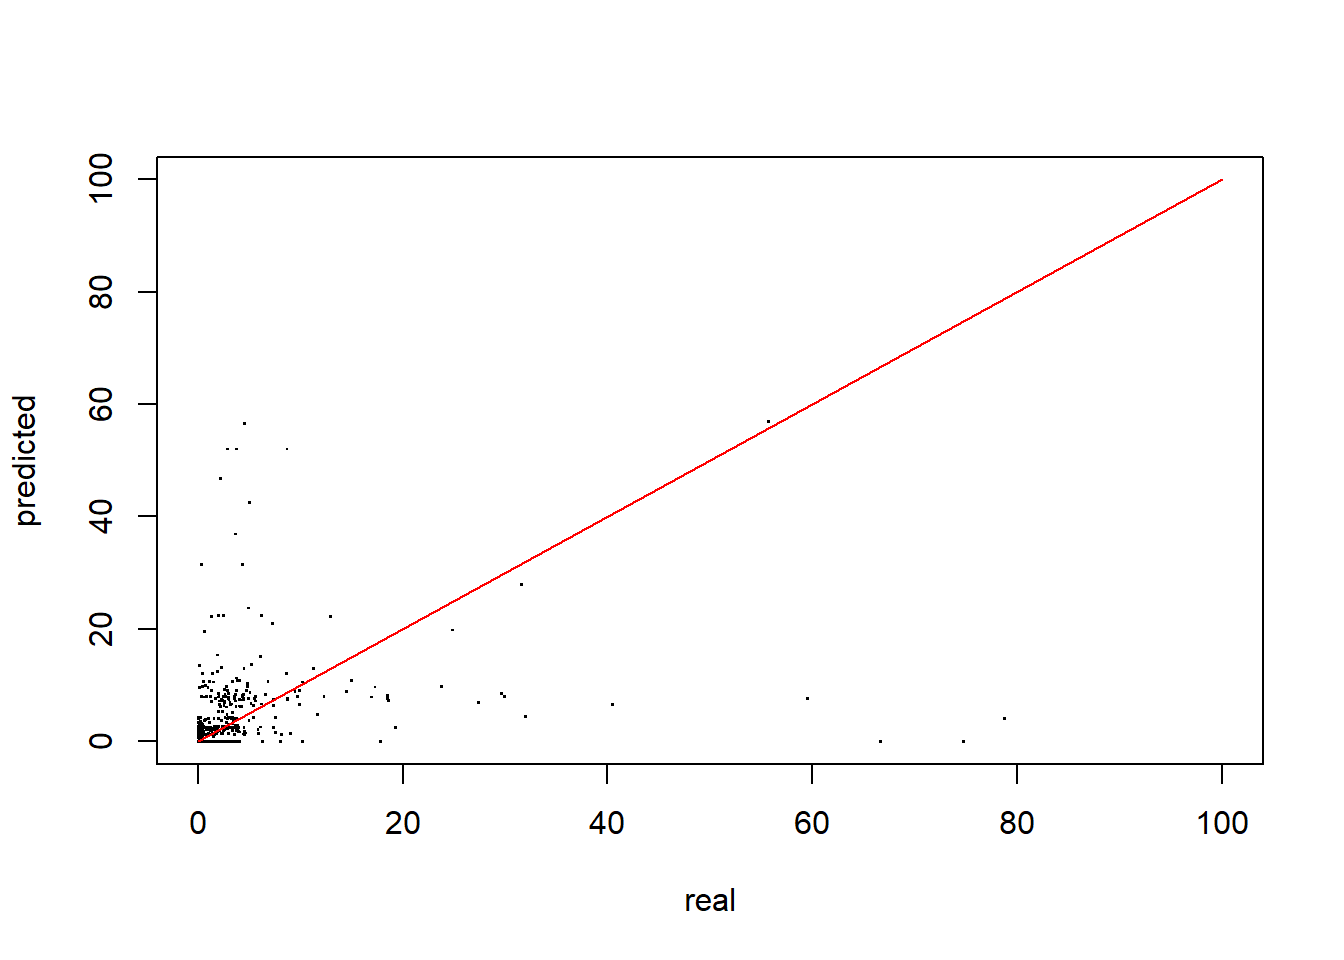
\includegraphics{02-Evaluation_files/figure-latex/unnamed-chunk-64-1.pdf}

\begin{quote}
Resumiendo
\end{quote}

Una función útil para medir el error:

\begin{Shaded}
\begin{Highlighting}[]
\KeywordTok{modelMetrics}\NormalTok{(}\DataTypeTok{real=}\NormalTok{modelchecktest1}\OperatorTok{$}\NormalTok{real, }\DataTypeTok{pred=}\NormalTok{modelchecktest1}\OperatorTok{$}\NormalTok{predicted )}
\end{Highlighting}
\end{Shaded}

\begin{verbatim}
##  Accuracy metrics (global):
\end{verbatim}

\begin{verbatim}
## MAE(ref) = 8.9208
\end{verbatim}

\begin{verbatim}
## MAE = 7.765
\end{verbatim}

\begin{verbatim}
## RMSE = 54.5686
\end{verbatim}

\begin{verbatim}
## MAPE = 127.01
\end{verbatim}

\begin{verbatim}
## MAPE(sim) = 68.65
\end{verbatim}

\begin{verbatim}
## WMAPE = 109.49
\end{verbatim}

\begin{itemize}
\tightlist
\item
  Commentario: El error de ajuste del modelo de regresión es demasiado alto: \(RMSE= 54.57\) y el \(MAPE=127.19%
  \)
  Con estos errores de predicción, es preferible utilizar a un modelo de clasificación en lugar de un modelo de regresión.
\end{itemize}

\textbf{Ejercicio sugerido}

\begin{itemize}
\item
  Ajustar un Modelo de Regresión Logística para \(Y\) y comparar los resultados con los proporcionados por el \emph{Random Forest}
\item
  Ajustar un Modelo de Regresión Lineal para \(LOSS\) y comparar los resultados con los proporcionados por el \emph{Random Forest}
\end{itemize}

\hypertarget{part-modelos-estadisticos}{%
\part{Modelos Estadísticos}\label{part-modelos-estadisticos}}

\hypertarget{regresion-lineal}{%
\chapter{Regresión Lineal}\label{regresion-lineal}}

\includegraphics{03-RegresionLineal_files/figure-latex/unnamed-chunk-2-1.pdf}

\includegraphics{03-RegresionLineal_files/figure-latex/unnamed-chunk-3-1.pdf}

Nota sobre \textbf{Modelo Estadístico}

\begin{itemize}
\item
  Los datos varian según las condiciones de su contexto experimental.
\item
  La \textbf{variabilidad} en los datos, puede ser expresada de manera simplificada a través de un modelo, conformado por una \textbf{ecuación} y una serie de \textbf{hipótesis} sobre las componentes de azar que subyacen el estudio.
\item
  La \textbf{ecuación} del modelo incluye siempre dos partes, una \textbf{determinísta} asociada con variaciones sistemáticas y que se reconoce que van a existir incluso antes de realizar el experimento y otra que depende de \textbf{componentes aleatorias} que son imposible de controlar y usualmente inherentes a la variabilidad propia del fenómeno aleatorio en estudio.

  \[ \text{Y} = \text{Funcion Deterministica} + \text{Perturbacion Aleatoria} \]
\item
  También se puede decir que en un modelo estadístico hay siempre dos estructuras íntimamente relacionadas:

  \begin{itemize}
  \tightlist
  \item
    La \textbf{estructura de media} (que provee el valor esperado para la respuesta bajo las condiciones experimentales)
  \item
    La \textbf{estructura de varianzas y covarianzas} (asociada a la o las componentes aleatorias del modelo).
  \end{itemize}
\end{itemize}

\hypertarget{que-es-un-modelo-de-regresion}{%
\section{¿Qué es un Modelo de Regresión?}\label{que-es-un-modelo-de-regresion}}

El modelo de regresión se utiliza para representar la relación entre \(Y\) y \(X\):
\[Y = f(x)\]

\begin{itemize}
\tightlist
\item
  \(Y\) es una variable respuesta, explicada o dependiente: que depende de otras y que tratamos de explicar/predecir.
\item
  \(X\), o mas bien \(X_1, X_2, \ldots, X_K\) son variables explicativas o independientes que permiten explicar/predecir \(Y\).
\end{itemize}

Una regresión es lineal, cuando la función \(f(x)\) que relaciona \(X\) e \(Y\) es una \textbf{función lineal}.

Teniendo \(K\) variables explicativas, la regresión lineal es:

\[ Y = \beta_0  + \beta_1 X_1 + \beta_2 X_2 + ... + \beta_K X_K + \epsilon; \epsilon \sim N(0,\sigma^2) \]

De manera que el valor de la predicción de la variable \(Y\) será:

\[ \hat{Y}  = \beta_0  + \beta_1 X_1 + \beta X_2 + ... + \beta X_K \]

O lo que es lo mismo:

\[  \epsilon = Y - \hat{Y} \]
Así, \(\epsilon\) será el error cometido en la previsión de \(Y\) usando el mode.

En función del número \(K\) de variables explicativas que tengamos, la regresión lineal puede ser \textbf{Simple} o \textbf{Múltiple}.

\begin{itemize}
\tightlist
\item
  \textbf{Simple} si hay una única variable independiente (\(K = 1\)).
\item
  \textbf{Múltiple} si hay varias variables independendientes (\(K > 1\)).
\end{itemize}

Para obtener la \(\hat{Y}\) es necesario conocer \(\beta_0, \ldots, \beta_K\), es decir, falta el proceso de \textbf{inferencia estadística}.

La \textbf{Inferencia Estadística} es el procedimiento que permiten elaborar conclusiones sobre parámetros poblacionales desconocidos.

\[ \hat{Y}  = \hat{\beta}_0  + \hat{\beta}_1 X_1 + \hat{\beta} X_2 + ... + \hat{\beta} X_K \]

\begin{itemize}
\tightlist
\item
  Conocer o estimar a un parámetro de la distribución de una variable es posible a través de un estadístico (estadístico muestral).
\item
  Dado que el estadístico es obtenido a partir de una muestra y hay más de una muestra posible de ser elegida, el valor del estadístico dependerá de la muestra seleccionada.
\item
  Como los valores de los estadísticos cambian de una muestra a otra. Interesa contar con una medida de estos cambios para cuantificar la medida del error en el que podría incurrirse al hacer una inferencia.
\end{itemize}

Los parámetros de un modelo de regresión se pueden estimar con:

\begin{itemize}
\tightlist
\item
  \textbf{Mínimos Cuadrados Ordinarios (OLS)}
\item
  \textbf{Máxima Verosimilitud (ML)}
\item
  \textbf{Inferencia Bayesiana}
\end{itemize}

\hypertarget{ver-tambien}{%
\subsection{Ver también:}\label{ver-tambien}}

\begin{itemize}
\item
  \href{http://reliawiki.org/index.php/Simple_Linear_Regression_Analysis}{Simple Linear Regression Analysis}
\item
  \href{https://www.maximaformacion.es/master-estadistica-aplicada-con-r/blog/item/como-validar-tu-modelo-de-regresion.html}{¿Cómo Validar Tu Modelo De Regresión?}
\item
  \href{https://www.maximaformacion.es/master-estadistica-aplicada-con-r/blog/item/que-modelo-de-regresion-deberia-elegir.html}{¿Qué modelo de regresión debería elegir?}
\item
  \href{https://www.maximaformacion.es/master-estadistica-aplicada-con-r/blog/item/como-seleccionar-las-variables-adecuadas-para-tu-modelo.html}{¿Cómo seleccionar las variables adecuadas para tu modelo?}
\end{itemize}

-\href{http://reliawiki.org/index.php/Multiple_Linear_Regression_Analysis}{Multiple Linear Regression Analysis}

\hypertarget{practica-en-r-1}{%
\section{Práctica en R}\label{practica-en-r-1}}

\hypertarget{regresion-lineal-simple}{%
\subsection{Regresión lineal simple}\label{regresion-lineal-simple}}

Para realizarla usaremos la base de datos \texttt{Boston} de la librería \texttt{MASS}.

\begin{Shaded}
\begin{Highlighting}[]
\KeywordTok{library}\NormalTok{(MASS)}
\end{Highlighting}
\end{Shaded}

Veamos la descripción de \texttt{Boston} en la ayuda de R:

\begin{Shaded}
\begin{Highlighting}[]
\NormalTok{?Boston}
\end{Highlighting}
\end{Shaded}

\begin{verbatim}
## starting httpd help server ... done
\end{verbatim}

Observamos que es un data.frame con 506 observaciones y 14 variables.

Podemos explorar un poco más los datos usando las funciones \texttt{head}, \texttt{tail} y \texttt{summary}.

\begin{Shaded}
\begin{Highlighting}[]
\KeywordTok{head}\NormalTok{(Boston,}\DecValTok{5}\NormalTok{)}
\end{Highlighting}
\end{Shaded}

\begin{verbatim}
##      crim zn indus chas   nox    rm  age    dis rad tax ptratio  black
## 1 0.00632 18  2.31    0 0.538 6.575 65.2 4.0900   1 296    15.3 396.90
## 2 0.02731  0  7.07    0 0.469 6.421 78.9 4.9671   2 242    17.8 396.90
## 3 0.02729  0  7.07    0 0.469 7.185 61.1 4.9671   2 242    17.8 392.83
## 4 0.03237  0  2.18    0 0.458 6.998 45.8 6.0622   3 222    18.7 394.63
## 5 0.06905  0  2.18    0 0.458 7.147 54.2 6.0622   3 222    18.7 396.90
##   lstat medv
## 1  4.98 24.0
## 2  9.14 21.6
## 3  4.03 34.7
## 4  2.94 33.4
## 5  5.33 36.2
\end{verbatim}

\begin{Shaded}
\begin{Highlighting}[]
\KeywordTok{tail}\NormalTok{(Boston,}\DecValTok{5}\NormalTok{)}
\end{Highlighting}
\end{Shaded}

\begin{verbatim}
##        crim zn indus chas   nox    rm  age    dis rad tax ptratio  black
## 502 0.06263  0 11.93    0 0.573 6.593 69.1 2.4786   1 273      21 391.99
## 503 0.04527  0 11.93    0 0.573 6.120 76.7 2.2875   1 273      21 396.90
## 504 0.06076  0 11.93    0 0.573 6.976 91.0 2.1675   1 273      21 396.90
## 505 0.10959  0 11.93    0 0.573 6.794 89.3 2.3889   1 273      21 393.45
## 506 0.04741  0 11.93    0 0.573 6.030 80.8 2.5050   1 273      21 396.90
##     lstat medv
## 502  9.67 22.4
## 503  9.08 20.6
## 504  5.64 23.9
## 505  6.48 22.0
## 506  7.88 11.9
\end{verbatim}

\begin{Shaded}
\begin{Highlighting}[]
\KeywordTok{summary}\NormalTok{(Boston)}
\end{Highlighting}
\end{Shaded}

\begin{verbatim}
##       crim                zn             indus            chas        
##  Min.   : 0.00632   Min.   :  0.00   Min.   : 0.46   Min.   :0.00000  
##  1st Qu.: 0.08204   1st Qu.:  0.00   1st Qu.: 5.19   1st Qu.:0.00000  
##  Median : 0.25651   Median :  0.00   Median : 9.69   Median :0.00000  
##  Mean   : 3.61352   Mean   : 11.36   Mean   :11.14   Mean   :0.06917  
##  3rd Qu.: 3.67708   3rd Qu.: 12.50   3rd Qu.:18.10   3rd Qu.:0.00000  
##  Max.   :88.97620   Max.   :100.00   Max.   :27.74   Max.   :1.00000  
##       nox               rm             age              dis        
##  Min.   :0.3850   Min.   :3.561   Min.   :  2.90   Min.   : 1.130  
##  1st Qu.:0.4490   1st Qu.:5.886   1st Qu.: 45.02   1st Qu.: 2.100  
##  Median :0.5380   Median :6.208   Median : 77.50   Median : 3.207  
##  Mean   :0.5547   Mean   :6.285   Mean   : 68.57   Mean   : 3.795  
##  3rd Qu.:0.6240   3rd Qu.:6.623   3rd Qu.: 94.08   3rd Qu.: 5.188  
##  Max.   :0.8710   Max.   :8.780   Max.   :100.00   Max.   :12.127  
##       rad              tax           ptratio          black       
##  Min.   : 1.000   Min.   :187.0   Min.   :12.60   Min.   :  0.32  
##  1st Qu.: 4.000   1st Qu.:279.0   1st Qu.:17.40   1st Qu.:375.38  
##  Median : 5.000   Median :330.0   Median :19.05   Median :391.44  
##  Mean   : 9.549   Mean   :408.2   Mean   :18.46   Mean   :356.67  
##  3rd Qu.:24.000   3rd Qu.:666.0   3rd Qu.:20.20   3rd Qu.:396.23  
##  Max.   :24.000   Max.   :711.0   Max.   :22.00   Max.   :396.90  
##      lstat            medv      
##  Min.   : 1.73   Min.   : 5.00  
##  1st Qu.: 6.95   1st Qu.:17.02  
##  Median :11.36   Median :21.20  
##  Mean   :12.65   Mean   :22.53  
##  3rd Qu.:16.95   3rd Qu.:25.00  
##  Max.   :37.97   Max.   :50.00
\end{verbatim}

Antes de continuar, hacemos la división de \texttt{Boston} en \texttt{train}y \texttt{test}.

\begin{Shaded}
\begin{Highlighting}[]
\NormalTok{id_train <-}\StringTok{ }\KeywordTok{sample}\NormalTok{(}\DecValTok{1}\OperatorTok{:}\KeywordTok{nrow}\NormalTok{(Boston), }\DataTypeTok{size =} \FloatTok{0.8}\OperatorTok{*}\KeywordTok{nrow}\NormalTok{(Boston))}
\NormalTok{train <-}\StringTok{ }\NormalTok{Boston[id_train, ]}
\NormalTok{test <-}\StringTok{ }\NormalTok{Boston[}\OperatorTok{-}\NormalTok{id_train, ]}
\end{Highlighting}
\end{Shaded}

Ajustamos el modelo de regresión lineal simple para predecir la variable \texttt{medv} utilizando la variable \texttt{lstat} de nuestro conjunto de datos \texttt{Boston}. Para ello usaremos la función \texttt{lm}.

\begin{Shaded}
\begin{Highlighting}[]
\NormalTok{reg_ls <-}\StringTok{ }\KeywordTok{lm}\NormalTok{(medv}\OperatorTok{~}\NormalTok{lstat, }\DataTypeTok{data =}\NormalTok{ train)}
\NormalTok{reg_ls}
\end{Highlighting}
\end{Shaded}

\begin{verbatim}
## 
## Call:
## lm(formula = medv ~ lstat, data = train)
## 
## Coefficients:
## (Intercept)        lstat  
##     34.1715      -0.9111
\end{verbatim}

Veamos los coeficientes de la regresión

\begin{Shaded}
\begin{Highlighting}[]
\NormalTok{reg_ls}\OperatorTok{$}\NormalTok{coefficients}
\end{Highlighting}
\end{Shaded}

\begin{verbatim}
## (Intercept)       lstat 
##  34.1715319  -0.9111111
\end{verbatim}

Donde el término independiente es:

\begin{Shaded}
\begin{Highlighting}[]
\NormalTok{reg_ls}\OperatorTok{$}\NormalTok{coefficients[}\DecValTok{1}\NormalTok{]}
\end{Highlighting}
\end{Shaded}

\begin{verbatim}
## (Intercept) 
##    34.17153
\end{verbatim}

y el coeficiente de la variable \texttt{lstat}es:

\begin{Shaded}
\begin{Highlighting}[]
\NormalTok{reg_ls}\OperatorTok{$}\NormalTok{coefficients[}\DecValTok{2}\NormalTok{]}
\end{Highlighting}
\end{Shaded}

\begin{verbatim}
##      lstat 
## -0.9111111
\end{verbatim}

De manera que la recta de regresión lineal, siendo \(y\) la variable \texttt{medv} y \(x\) la variable \texttt{lstat}, es:

\begin{verbatim}
## y =  34.17153 +  -0.9111111 x
\end{verbatim}

Si queremos obtener los errores residuales de las observaciones correspondientes:

\begin{Shaded}
\begin{Highlighting}[]
\NormalTok{residuales <-}\StringTok{ }\NormalTok{reg_ls}\OperatorTok{$}\NormalTok{residuals}
\CommentTok{# Veamos los residuales de las 10 primeras observaciones}
\NormalTok{residuales[}\DecValTok{1}\OperatorTok{:}\DecValTok{10}\NormalTok{]}
\end{Highlighting}
\end{Shaded}

\begin{verbatim}
##        324        503        350        377        167        133 
## -4.9750880 -5.2986434 -2.2050877  0.9026893 19.1995790 -1.0399768 
##        213        157        316        469 
##  2.8335785 -6.3661993 -7.4937546  1.4469118
\end{verbatim}

Una vez obtenido el modelo de regresión lineal, para realizar la predicción sobre un nuevo conjunto de datos, utilizamos la función \texttt{predict}, de la siguiente manera:

\begin{Shaded}
\begin{Highlighting}[]
\NormalTok{predic <-}\StringTok{ }\KeywordTok{predict}\NormalTok{(reg_ls, }\DataTypeTok{newdata =}\NormalTok{ test)}
\CommentTok{#Veamos la predicción de las 10 primeras observaciones}
\NormalTok{predic[}\DecValTok{1}\OperatorTok{:}\DecValTok{10}\NormalTok{]}
\end{Highlighting}
\end{Shaded}

\begin{verbatim}
##       11       14       19       21       22       23       28       34 
## 15.53931 26.64575 23.52064 15.01998 21.57087 17.11553 18.42753 17.45264 
##       38       44 
## 26.18109 27.39287
\end{verbatim}

Algunas representaciones gráficas de un modelo de regresión son:

\begin{itemize}
\tightlist
\item
  Dispersión de los puntos y la recta de regresión lineal simple obtenida:
\end{itemize}

\begin{Shaded}
\begin{Highlighting}[]
\NormalTok{regresion <-}\StringTok{ }\KeywordTok{lm}\NormalTok{(medv}\OperatorTok{~}\NormalTok{lstat, }\DataTypeTok{data =}\NormalTok{ Boston)}

\KeywordTok{plot}\NormalTok{(Boston}\OperatorTok{$}\NormalTok{lstat, Boston}\OperatorTok{$}\NormalTok{medv, }\DataTypeTok{xlab =} \StringTok{"lstat"}\NormalTok{, }\DataTypeTok{ylab =} \StringTok{"medv"}\NormalTok{)}
\KeywordTok{abline}\NormalTok{(regresion, }\DataTypeTok{col=}\StringTok{'red'}\NormalTok{, }\DataTypeTok{lwd=}\DecValTok{2}\NormalTok{)}
\NormalTok{a <-}\StringTok{ }\NormalTok{regresion}\OperatorTok{$}\NormalTok{coefficients[[}\DecValTok{1}\NormalTok{]]}
\NormalTok{b <-}\StringTok{ }\NormalTok{regresion}\OperatorTok{$}\NormalTok{coefficients[[}\DecValTok{2}\NormalTok{]] }
\KeywordTok{text}\NormalTok{(}\DecValTok{30}\NormalTok{,}\DecValTok{40}\NormalTok{,}\DataTypeTok{labels =} \KeywordTok{paste}\NormalTok{(}\StringTok{'Y = '}\NormalTok{, }\KeywordTok{round}\NormalTok{(b,}\DecValTok{2}\NormalTok{),}\StringTok{'x +'}\NormalTok{, }\KeywordTok{round}\NormalTok{(a,}\DecValTok{2}\NormalTok{)), }\DataTypeTok{col=}\StringTok{'red'}\NormalTok{)}
\end{Highlighting}
\end{Shaded}

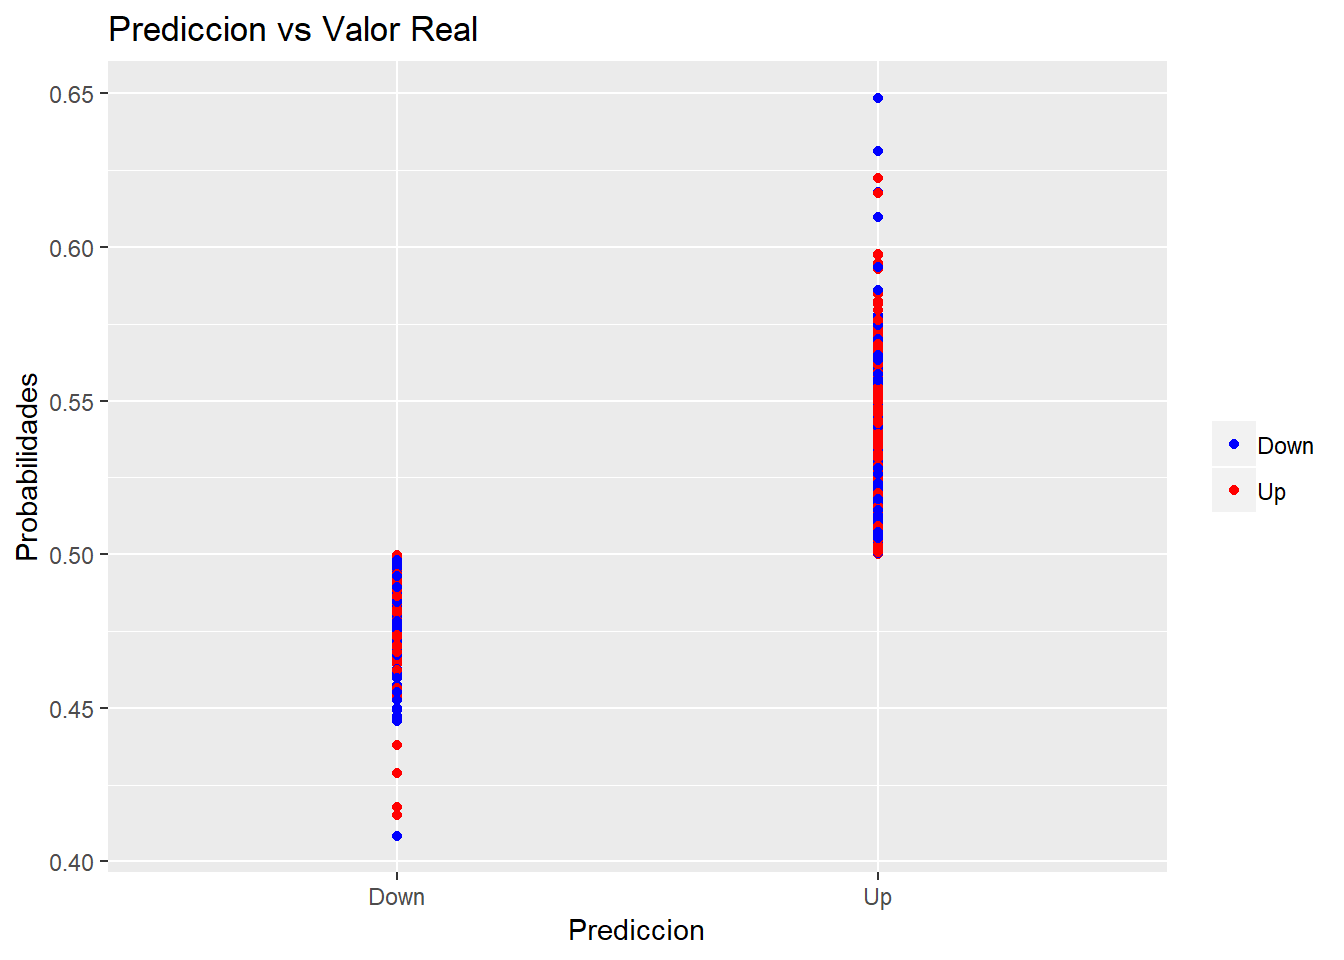
\includegraphics{03-RegresionLineal_files/figure-latex/unnamed-chunk-17-1.pdf}

\begin{itemize}
\tightlist
\item
  Análisis de residuos:
\end{itemize}

\begin{Shaded}
\begin{Highlighting}[]
\KeywordTok{par}\NormalTok{(}\DataTypeTok{mfrow=}\KeywordTok{c}\NormalTok{(}\DecValTok{2}\NormalTok{,}\DecValTok{2}\NormalTok{))}
\KeywordTok{plot}\NormalTok{(regresion)}
\end{Highlighting}
\end{Shaded}

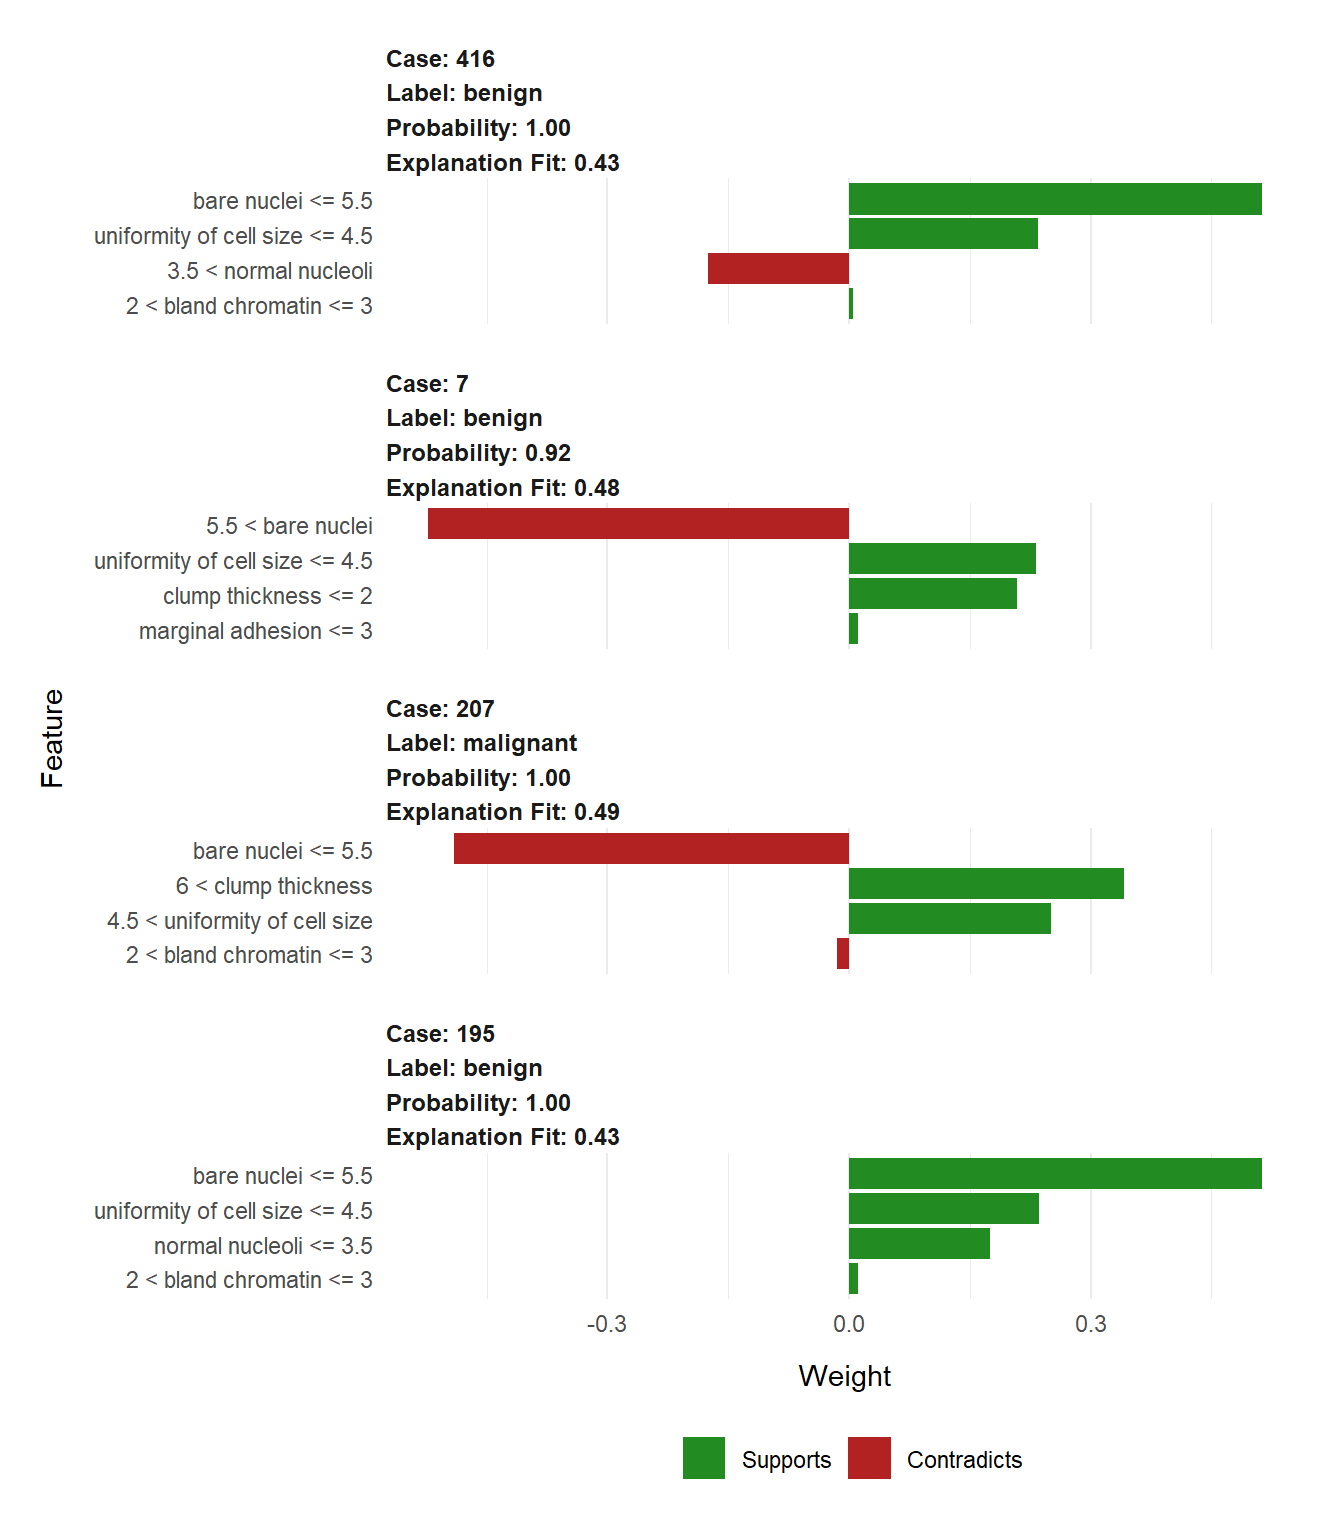
\includegraphics{03-RegresionLineal_files/figure-latex/unnamed-chunk-18-1.pdf}

\hypertarget{regresion-lineal-multiple}{%
\subsection{Regresión lineal múltiple}\label{regresion-lineal-multiple}}

Utilizamos lo mismo que hemos hecho para la regresión lineal simple, con la diferencia de que ahora hay más de una variable independiente.
Usamos la misma función, \texttt{lm}, y la sucesión de variables independientes estarán separadas con un \texttt{+}, es decir:

\begin{Shaded}
\begin{Highlighting}[]
\NormalTok{reg_lm <-}\StringTok{ }\KeywordTok{lm}\NormalTok{(medv}\OperatorTok{~}\NormalTok{lstat }\OperatorTok{+}\StringTok{ }\NormalTok{age, }\DataTypeTok{data =}\NormalTok{ train)}
\NormalTok{reg_lm}
\end{Highlighting}
\end{Shaded}

\begin{verbatim}
## 
## Call:
## lm(formula = medv ~ lstat + age, data = train)
## 
## Coefficients:
## (Intercept)        lstat          age  
##    32.84634     -0.98562      0.03292
\end{verbatim}

Veamos los coeficientes de la regresión

\begin{Shaded}
\begin{Highlighting}[]
\NormalTok{reg_lm}\OperatorTok{$}\NormalTok{coefficients}
\end{Highlighting}
\end{Shaded}

\begin{verbatim}
## (Intercept)       lstat         age 
## 32.84634095 -0.98562034  0.03292455
\end{verbatim}

Donde el término independiente es:

\begin{Shaded}
\begin{Highlighting}[]
\NormalTok{reg_lm}\OperatorTok{$}\NormalTok{coefficients[}\DecValTok{1}\NormalTok{]}
\end{Highlighting}
\end{Shaded}

\begin{verbatim}
## (Intercept) 
##    32.84634
\end{verbatim}

el coeficiente de la variable \texttt{lstat} es:

\begin{Shaded}
\begin{Highlighting}[]
\NormalTok{reg_lm}\OperatorTok{$}\NormalTok{coefficients[}\DecValTok{2}\NormalTok{]}
\end{Highlighting}
\end{Shaded}

\begin{verbatim}
##      lstat 
## -0.9856203
\end{verbatim}

y el coeficiente de la variable \texttt{age} es:

\begin{Shaded}
\begin{Highlighting}[]
\NormalTok{reg_lm}\OperatorTok{$}\NormalTok{coefficients[}\DecValTok{3}\NormalTok{]}
\end{Highlighting}
\end{Shaded}

\begin{verbatim}
##        age 
## 0.03292455
\end{verbatim}

De manera que la recta de regresión lineal, siendo \(y\) la variable \texttt{medv}, \(x1\) la variable \texttt{lstat} y \(x2\) la variable \texttt{age}, será:

\begin{verbatim}
## y =  32.84634 +  -0.9856203 x1 + 0.03292455 x2
\end{verbatim}

Veamos los gráficos de dispersión 2 a 2:

\begin{Shaded}
\begin{Highlighting}[]
\KeywordTok{pairs}\NormalTok{(Boston[,}\KeywordTok{c}\NormalTok{(}\StringTok{'medv'}\NormalTok{,}\StringTok{'lstat'}\NormalTok{, }\StringTok{'age'}\NormalTok{)],}\DataTypeTok{panel =}\NormalTok{ panel.smooth)}
\end{Highlighting}
\end{Shaded}

\includegraphics{03-RegresionLineal_files/figure-latex/{]}-1.pdf}

Análogamente a como hemos hecho con la regresión lineal, podemos obtener los residuos y utilizar la función \texttt{predict} en un nuevo conjunto de datos.

Hay otras opciones de poner la variables independientes. Por ejemplo, si quisieramos usar todas las variables, como conjunto de variables independientes, bastaría con escribir:

\begin{Shaded}
\begin{Highlighting}[]
\NormalTok{reg_lm2 <-}\StringTok{ }\KeywordTok{lm}\NormalTok{(medv}\OperatorTok{~}\NormalTok{., }\DataTypeTok{data =}\NormalTok{ train)}
\NormalTok{reg_lm2}
\end{Highlighting}
\end{Shaded}

\begin{verbatim}
## 
## Call:
## lm(formula = medv ~ ., data = train)
## 
## Coefficients:
## (Intercept)         crim           zn        indus         chas  
##   43.865429    -0.106094     0.045046    -0.034204     3.122022  
##         nox           rm          age          dis          rad  
##  -19.830234     3.184818     0.003712    -1.695735     0.306205  
##         tax      ptratio        black        lstat  
##   -0.011510    -0.984545     0.007409    -0.534384
\end{verbatim}

Por otro lado, si quisieramos usarlas todas excepto alguna, podemos escribir:

\begin{Shaded}
\begin{Highlighting}[]
\NormalTok{reg_lm3 <-}\StringTok{ }\KeywordTok{lm}\NormalTok{(medv}\OperatorTok{~}\NormalTok{.}\OperatorTok{-}\NormalTok{age, }\DataTypeTok{data =}\NormalTok{ train)}
\NormalTok{reg_lm3}
\end{Highlighting}
\end{Shaded}

\begin{verbatim}
## 
## Call:
## lm(formula = medv ~ . - age, data = train)
## 
## Coefficients:
## (Intercept)         crim           zn        indus         chas  
##   43.767647    -0.105721     0.044539    -0.033702     3.130323  
##         nox           rm          dis          rad          tax  
##  -19.551080     3.205457    -1.711176     0.305140    -0.011495  
##     ptratio        black        lstat  
##   -0.981650     0.007475    -0.530236
\end{verbatim}

\hypertarget{regresion-logistica}{%
\chapter{Regresión Logística}\label{regresion-logistica}}

Una aplicación muy conocida son los modelos de \textbf{churn}. Un modelo de churn es una herramienta que permite evaluar la \textbf{probabilidad de baja o fuga} de un cliente en función de sus características propias y del tipo de relación que tiene con la empresa.

La variable que se analiza toma valor 1 ó 0. Para representar la relación entre esa \textbf{variable binaria} (output) y las variables explicativas (inputs), se utilizan modelos de tipo \textless{}font \textbf{logit} o \textbf{probit}.

\hypertarget{modelos-lineales-generalizados}{%
\section{Modelos Lineales Generalizados}\label{modelos-lineales-generalizados}}

Los Modelos Lineales Generalizados son una extensión de los modelos lineales
clásicos. Un modelo lineal se basa en un vector de observaciones \(\mathbf{Y}\) con \(n\) componentes,
que son una realización de una variable aleatoria \(\mathbf{Y}\) cuyas componentes están independientemente distribuidas con media \(\mu\). Un modelo lineal puede ser descrito
como:
\[\mathbf{Y} = \mathbf{\mu} + \mathbf{\epsilon}\]

La parte sistemática de un modelo es una especificación para \(\mu\) en función de un número pequeño de parámetros, \(\beta_1, \ldots, \beta_p.\) Esa especificación se hace de la siguiente manera:
\[
\mu_i = \sum_{j=1}^p  X_{ij}\beta_j;     i=1,\ldots,n.
\]

O en forma matricial,
\[
E(\mathbf{Y}) = \mathbf{\mu} = \mathbf{x} \mathbf{\beta}
\]

donde \(\mathbf{X}\) es una matriz \(n \times p\), con las covariables o regresoras del modelo. Para la parte aleatoria se supone independencia y varianza constante de los errores.

En un modelo lineal clásico, se tiene que:
\[
\mathbf{\epsilon} \sim N(0, \sigma^2 \mathbf{I})
\]

Por tanto un modelo lineal clásico puede ser resumido de la forma:
\[
\begin{align}
        \mathbf{Y} & \sim N(\mathbf{\mu}, \sigma^2 \mathbf{I}) \\
        E(\mathbf{Y}) & = \mathbf{X}\mathbf{\beta} \\
        Var(\mathbf{Y}) & =  \sigma^2\mathbf{I}
\end{align}
\]

La generalización de los modelos lineales incluye una especificación de tres aspectos principales:

\begin{itemize}
\tightlist
\item
  Las componentes de \(\mathbf{Y}\) tienen distribución normal con varianza constante y son independientes.
\item
  En la parte sistemática, las covariables, \(x_1, x_2, ..., x_p\), producen un predictor
  lineal \(\eta\), dado por:
\end{itemize}

\[ \eta= \sum_{j=1}^p  X_{ij}\beta_j \]

\begin{itemize}
\tightlist
\item
  La relación entre los componentes sistemáticos y aleatorios se hace a través de una función de manera que:
\end{itemize}

\[\mathbf{\mu}=\mathbf{\eta}\]

Los Modelos Lineales Generalizados o MLGs permiten dos extensiones. La primera extensión está en la función de enlace, que es la parte del modelo que determina la relación entre la media de la variable respuesta y las covariables. Esta función de enlace, ahora, podrá ser cualquier función monótona diferenciable y generalmente denotada por \(g(\mu)\). La segunda extensión reside en la distribución especificada para la componente aleatoria. En los MLGs esta puede ser de la familia exponencial, de la cual la distribución normal forma parte.

Se supone que si \(\mathbf{Y}\) tiene una distribución de la familia exponencial para unos específicos \(a(\cdot), b(\cdot)\) y \(c(\cdot)\) se asume la siguiente forma:

\[
f_Y ( \mathbf{Y} | \eta,\phi) = \exp \left\{ \dfrac{\mathbf{\eta} - b(\eta)}{a(\phi)} + c(\mathbf{Y},\phi) \right\}
\]

El parámetro \(\phi\) es llamado parámetro de dispersión y, si es conocido, llamamos a su familia ``de familia exponencial lineal de parámetro canónico \(\theta\)''. Utilizando la ecuación anterior y algunas relaciones, se puede obtener expresiones para la media y la varianza de \(\mathbf{Y}\) de la siguiente manera:

\[
\begin{align}
        E(\mathbf{Y}) & = b'(\eta) \\
        Var(\mathbf{Y}) & =  a(\phi)b''(\eta)
\end{align}
\]

\hypertarget{modelo-logit}{%
\section{Modelo Logit}\label{modelo-logit}}

Cuando la variable respuesta es continua, se utilizan métodos de regresión lineal o de otro tipo; en cambio, cuando la \textbf{variable respuesta es cualitativa} se utilizan los llamados \textbf{Modelos de Regresión Logística}.

El objetivo de los modelos de regresión logística es encontrar el mejor ajuste para describir las relaciones entre las variables respuesta (dicotómica o cualitativa) y un grupo de variables explicativas. Esta diferencia (respecto a los modelos con variable respuesta cuantitativa) da lugar a distintos modelos paramétricos y a distintas hipótesis para estos modelos, pero, una vez salvada esta diferencia, los métodos empleados en Regresión Logística siguen los principios generales de los métodos de Regresión Lineal.

La primera razón por la cual un Modelo de Regresión Lineal no es adecuado para este tipo de datos es que la \textbf{variable respuesta sólo puede tomar 2 valores (0 y 1)}, de modo que si pretendiésemos elaborar una relación entre una variable explicativa y esta, tendríamos que condicionar la probabilidad de alguno de los valores de la variable respuesta a cada valor de la variable explicativa, es decir
\(E(Y= 1 | X = x_1)\) y obtendríamos la \textbf{curva logística}:

\includegraphics{04-RegresionLogistica_files/figure-latex/unnamed-chunk-2-1.pdf}

La relación existente no es lineal, sino que puede asociarse con la función de distribución de cierta variable aleatoria. Al utilizar la distribución Logística, representaremos la media de \(Y\), dado un valor \(x\) de la variable \(X\), por \(\pi(X)=E(Y/x)\).

El modelo de Regresión Logística es:
\[
\pi(x) = \frac{e^{\beta_0+\beta_1x}}{1+e^{\beta_0+\beta_1x}}
\]
o de forma equivalente:
\[ \pi(x) = \frac{1}{1 + e^{-(\beta_0 + \beta_1 x)}} \]

Aplicando la transformación Logit:
\[
g(x)=\ln\Big[\frac{\pi(x)}{1-\pi(x)}\Big]= \beta_0+\beta_1x
\]

Hemos llegado a \(g(x)\), que tiene las propiedades que se desea que tenga un Modelo de Regresión Lineal; es lineal en sus parámetros; puede ser continua y su rango está entre \(-\infty\) y \(\infty\) dependiendo del rango de X.

Como hemos dicho antes, también tenemos que tener clara la distribución de la parte aleatoria de nuestro modelo. En el Modelo Lineal Generalizado suponemos que un valor de la variable dependiente puede expresarse como \(y=E(Y/x)+\epsilon.\) Donde \(\epsilon\sim N(0,\sigma^2)\), con varianza constante para los distintos niveles de la variable independiente. Pero esto no ocurre así en el caso de una variable dicotómica.

Si expresamos nuestro modelo como \(Y = \pi(x) + \epsilon,\) \(\epsilon\) toma dos posibles valores:

\begin{itemize}
\tightlist
\item
  Si \(Y=1,\) con probabilidad \(\pi(x)\), \(\epsilon= 1-\pi(x)\), con probabilidad \(\pi(x)\).
\item
  Si \(Y=0, \epsilon = -\pi(x)\), con probabilidad \(1-\pi(x)\).
\end{itemize}

Por tanto:
\[
E(\epsilon)= (1-\pi(x))\pi(x)-\pi(x)(1-\pi(x))=0
\]

\[
V(\epsilon) = (1-\pi(x))^2\pi(x)-\pi(x))^2(1-\pi(x))=\pi(x)(1-\pi(x))
\]

La distribución de la variable dependiente \(Y\), dado un valor de \(x\) de la variable \(X\), sigue una distribución Binomial con probabilidad \(\pi(x)\).

Al no ser una relación lineal, no es posible interpretar directamente el valor de los parámetros estimados.
Para ello se utilizan los \emph{`ODDS Ratios'}.

A través de un ratio de ODDS se puede calcular qué influencia genera en el target el incremento de una unidad en el valor de la variable explicativa.

\begin{itemize}
\tightlist
\item
  Si \(\beta_i > 0\) el efecto de la variable explicativa \(X_i\) sobre la respuesta \(Y\) es de incremento: aumenta la probabilidad del target.
\item
  Si \(\beta_i < 0\) el efecto que produce la variable explicativa \(X_i\) sobre la respuesta \(Y\) es decremento: disminuye la probabilidad del target.
\end{itemize}

\hypertarget{modelo-probit}{%
\section{Modelo Probit}\label{modelo-probit}}

La relación existente entre \(E(Y= 1/X=x_1)\) y \(X\), que como dicho anteriormente no es linea, se asocia también con la curva de distribución normal.Este enfoque utiliza la inversa de la función de distribución normal para obtener una relación lineal entre \(E(Y= 1/X=x_1)\) y \(X\). Y una vez hayamos tenido los valores en forma de relación lineal del tipo \(g(x) = B_0+B_1x_1\) volveremos a transformarlo en una curva que se asemeje a una distribución aleatoria de la siguiente manera:

\[
E(Y=1/X) = \int_{-\infty}^{B_0+B_1 x_1}\frac{1}{\sqrt{2\pi}}e^{\frac{-z^2}{2}}
\]

Así estimando los valores de \(B_0\) y \(B_1\), siguiendo el proceso anteriormente mencionado, obtendremos estimaciones de las probabilidades de un determinado valor de la variable respuesta \((Y)\) condicionada a unos determinados valores de las variables explicativas \((X_1,X_2,...X_n)\).

\hypertarget{practica-en-r-2}{%
\section{Práctica en R}\label{practica-en-r-2}}

Para este ejemplo cargamos la librería \texttt{ISLR} y utilizamos el conjunto de datos de \texttt{Smarket}.

Veamos información sobre los datos \texttt{Smarket}

\begin{Shaded}
\begin{Highlighting}[]
\NormalTok{?Smarket}
\end{Highlighting}
\end{Shaded}

\begin{verbatim}
## starting httpd help server ... done
\end{verbatim}

\begin{Shaded}
\begin{Highlighting}[]
\KeywordTok{head}\NormalTok{(Smarket)}
\end{Highlighting}
\end{Shaded}

\begin{verbatim}
##   Year   Lag1   Lag2   Lag3   Lag4   Lag5 Volume  Today Direction
## 1 2001  0.381 -0.192 -2.624 -1.055  5.010 1.1913  0.959        Up
## 2 2001  0.959  0.381 -0.192 -2.624 -1.055 1.2965  1.032        Up
## 3 2001  1.032  0.959  0.381 -0.192 -2.624 1.4112 -0.623      Down
## 4 2001 -0.623  1.032  0.959  0.381 -0.192 1.2760  0.614        Up
## 5 2001  0.614 -0.623  1.032  0.959  0.381 1.2057  0.213        Up
## 6 2001  0.213  0.614 -0.623  1.032  0.959 1.3491  1.392        Up
\end{verbatim}

\begin{Shaded}
\begin{Highlighting}[]
\KeywordTok{summary}\NormalTok{(Smarket)}
\end{Highlighting}
\end{Shaded}

\begin{verbatim}
##       Year           Lag1                Lag2          
##  Min.   :2001   Min.   :-4.922000   Min.   :-4.922000  
##  1st Qu.:2002   1st Qu.:-0.639500   1st Qu.:-0.639500  
##  Median :2003   Median : 0.039000   Median : 0.039000  
##  Mean   :2003   Mean   : 0.003834   Mean   : 0.003919  
##  3rd Qu.:2004   3rd Qu.: 0.596750   3rd Qu.: 0.596750  
##  Max.   :2005   Max.   : 5.733000   Max.   : 5.733000  
##       Lag3                Lag4                Lag5         
##  Min.   :-4.922000   Min.   :-4.922000   Min.   :-4.92200  
##  1st Qu.:-0.640000   1st Qu.:-0.640000   1st Qu.:-0.64000  
##  Median : 0.038500   Median : 0.038500   Median : 0.03850  
##  Mean   : 0.001716   Mean   : 0.001636   Mean   : 0.00561  
##  3rd Qu.: 0.596750   3rd Qu.: 0.596750   3rd Qu.: 0.59700  
##  Max.   : 5.733000   Max.   : 5.733000   Max.   : 5.73300  
##      Volume           Today           Direction 
##  Min.   :0.3561   Min.   :-4.922000   Down:602  
##  1st Qu.:1.2574   1st Qu.:-0.639500   Up  :648  
##  Median :1.4229   Median : 0.038500             
##  Mean   :1.4783   Mean   : 0.003138             
##  3rd Qu.:1.6417   3rd Qu.: 0.596750             
##  Max.   :3.1525   Max.   : 5.733000
\end{verbatim}

En este caso la variable \texttt{Y} que queremos predecir/explicar es la variable \texttt{Direction}, y las variables independientes son \texttt{Lag1}, \texttt{Lag2}, \texttt{Lag3}, \texttt{Lag4}, \texttt{Lag5} y \texttt{Volume}.

Veamos que valores toma la variable \texttt{Direction}

\begin{Shaded}
\begin{Highlighting}[]
\KeywordTok{levels}\NormalTok{(Smarket}\OperatorTok{$}\NormalTok{Direction)}
\end{Highlighting}
\end{Shaded}

\begin{verbatim}
## [1] "Down" "Up"
\end{verbatim}

Vemos que es una variable binaria que toma valores \texttt{Down}o \texttt{Up}.
Antes de continuar pasamos esos valores a \texttt{0} o \texttt{1}, respectivamente.

\begin{Shaded}
\begin{Highlighting}[]
\NormalTok{Smarket}\OperatorTok{$}\NormalTok{Direction <-}\StringTok{ }\KeywordTok{ifelse}\NormalTok{(Smarket}\OperatorTok{$}\NormalTok{Direction }\OperatorTok{==}\StringTok{ 'Up'}\NormalTok{, }\DecValTok{1}\NormalTok{, }\DecValTok{0}\NormalTok{)}
\end{Highlighting}
\end{Shaded}

Para realizar la regresión logística en R utilizaremos la función \texttt{glm}.
Se puede observar en el código siguiente, que como nuestro Target es binario, el parámetro \texttt{family} lo debemos fijar a binomial.

\begin{Shaded}
\begin{Highlighting}[]
\NormalTok{reg_logis <-}\StringTok{ }\KeywordTok{glm}\NormalTok{(Direction}\OperatorTok{~}\NormalTok{Lag1 }\OperatorTok{+}\StringTok{ }\NormalTok{Lag2 }\OperatorTok{+}\StringTok{ }\NormalTok{Lag3 }\OperatorTok{+}\StringTok{ }\NormalTok{Lag4 }\OperatorTok{+}\StringTok{ }\NormalTok{Lag5 }\OperatorTok{+}\StringTok{ }\NormalTok{Volume,}
                 \DataTypeTok{data =}\NormalTok{ Smarket,}
                 \DataTypeTok{family =}\NormalTok{ binomial)}
\end{Highlighting}
\end{Shaded}

Veamos que hemos obtenido

\begin{Shaded}
\begin{Highlighting}[]
\KeywordTok{summary}\NormalTok{(reg_logis)}
\end{Highlighting}
\end{Shaded}

\begin{verbatim}
## 
## Call:
## glm(formula = Direction ~ Lag1 + Lag2 + Lag3 + Lag4 + Lag5 + 
##     Volume, family = binomial, data = Smarket)
## 
## Deviance Residuals: 
##    Min      1Q  Median      3Q     Max  
## -1.446  -1.203   1.065   1.145   1.326  
## 
## Coefficients:
##              Estimate Std. Error z value Pr(>|z|)
## (Intercept) -0.126000   0.240736  -0.523    0.601
## Lag1        -0.073074   0.050167  -1.457    0.145
## Lag2        -0.042301   0.050086  -0.845    0.398
## Lag3         0.011085   0.049939   0.222    0.824
## Lag4         0.009359   0.049974   0.187    0.851
## Lag5         0.010313   0.049511   0.208    0.835
## Volume       0.135441   0.158360   0.855    0.392
## 
## (Dispersion parameter for binomial family taken to be 1)
## 
##     Null deviance: 1731.2  on 1249  degrees of freedom
## Residual deviance: 1727.6  on 1243  degrees of freedom
## AIC: 1741.6
## 
## Number of Fisher Scoring iterations: 3
\end{verbatim}

Los coeficientes de la regresión logística obtenida serán:

\begin{Shaded}
\begin{Highlighting}[]
\KeywordTok{coef}\NormalTok{(reg_logis)}
\end{Highlighting}
\end{Shaded}

\begin{verbatim}
##  (Intercept)         Lag1         Lag2         Lag3         Lag4 
## -0.126000257 -0.073073746 -0.042301344  0.011085108  0.009358938 
##         Lag5       Volume 
##  0.010313068  0.135440659
\end{verbatim}

Como se hace en los otros modelos, la función \texttt{predict} la utilizaremos para predecir un nuevo conjunto de datos a partir de nuestro modelo de regresión logística ajustado.

Para un modelo binomial predeterminado, las predicciones serán de log-odds (probabilidades en la escala logit). Como vemos en el código a continuación, utilizamos el argumento \texttt{type\ =\ response} para guardar la predicción de las probabilidades.

\begin{Shaded}
\begin{Highlighting}[]
\NormalTok{glm.probs <-}\StringTok{ }\KeywordTok{predict}\NormalTok{(reg_logis,}
                     \DataTypeTok{type =}  \StringTok{"response"}\NormalTok{)}
\end{Highlighting}
\end{Shaded}

Lo que hacemos a continuación es dar a una observación el valor del target \(1\) o \(0\) en función a la probabilidad obtenida. El corte en la probabilidad en este caso lo ponemos en \(0.5\), es decir, si la predicción que se ha obtenido de la probabilidad es menor que 0.5, le damos el valor \(0\), y sino el valor \(1\). El código que hace esto es de la siguiente manera:

\begin{Shaded}
\begin{Highlighting}[]
\NormalTok{glm.pred <-}\StringTok{ }\KeywordTok{rep}\NormalTok{(}\DecValTok{1}\NormalTok{, }\KeywordTok{nrow}\NormalTok{(Smarket))}
\NormalTok{glm.pred[glm.probs }\OperatorTok{<}\StringTok{ }\FloatTok{.5}\NormalTok{] <-}\StringTok{ }\DecValTok{0}
\end{Highlighting}
\end{Shaded}

Ahora, obtenemos la \textbf{matriz de confusión}, en el que podemos comparar el valor de la predicción obtenida (filas) con el verdadero valor (columnas). De esta manera, lo que está en la diagonal principal será lo que se ha predecido correctamente.

\begin{Shaded}
\begin{Highlighting}[]
\KeywordTok{table}\NormalTok{(glm.pred, Smarket}\OperatorTok{$}\NormalTok{Direction) }
\end{Highlighting}
\end{Shaded}

\begin{verbatim}
##         
## glm.pred   0   1
##        0 145 141
##        1 457 507
\end{verbatim}

observamos la media de los valores que se ha predecido bien:

\begin{Shaded}
\begin{Highlighting}[]
\KeywordTok{mean}\NormalTok{(glm.pred }\OperatorTok{==}\StringTok{ }\NormalTok{Smarket}\OperatorTok{$}\NormalTok{Direction)}
\end{Highlighting}
\end{Shaded}

\begin{verbatim}
## [1] 0.5216
\end{verbatim}

y la media de los que se han predecido mal:

\begin{Shaded}
\begin{Highlighting}[]
\KeywordTok{mean}\NormalTok{(glm.pred }\OperatorTok{!=}\StringTok{ }\NormalTok{Smarket}\OperatorTok{$}\NormalTok{Direction)}
\end{Highlighting}
\end{Shaded}

\begin{verbatim}
## [1] 0.4784
\end{verbatim}

Podemos ver de manera gráfica como han sido clasificados por nuestro modelo (en función de la probabilidad obtenida) frente a su valor real.

\begin{Shaded}
\begin{Highlighting}[]
\NormalTok{nuevo <-}\StringTok{ }\KeywordTok{data.frame}\NormalTok{(glm.probs, glm.pred, Smarket}\OperatorTok{$}\NormalTok{Direction)}
\KeywordTok{names}\NormalTok{(nuevo)[}\DecValTok{1}\NormalTok{] <-}\StringTok{ "probs"}
\KeywordTok{names}\NormalTok{(nuevo)[}\DecValTok{2}\NormalTok{] <-}\StringTok{ "pred"}
\KeywordTok{names}\NormalTok{(nuevo)[}\DecValTok{3}\NormalTok{] <-}\StringTok{ "direction"}

\NormalTok{nuevo}\OperatorTok{$}\NormalTok{direction <-}\StringTok{ }\KeywordTok{ifelse}\NormalTok{(nuevo}\OperatorTok{$}\NormalTok{direction }\OperatorTok{==}\StringTok{ }\DecValTok{1}\NormalTok{, }\StringTok{'Up'}\NormalTok{, }\StringTok{'Down'}\NormalTok{)}
\NormalTok{nuevo}\OperatorTok{$}\NormalTok{pred <-}\StringTok{ }\KeywordTok{ifelse}\NormalTok{(nuevo}\OperatorTok{$}\NormalTok{pred }\OperatorTok{==}\StringTok{ }\DecValTok{1}\NormalTok{, }\StringTok{'Up'}\NormalTok{, }\StringTok{'Down'}\NormalTok{)}
\KeywordTok{library}\NormalTok{(ggplot2)}
\KeywordTok{ggplot}\NormalTok{(}\DataTypeTok{data =}\NormalTok{ nuevo, }
       \KeywordTok{aes}\NormalTok{(}\DataTypeTok{x =}\NormalTok{ pred, }\DataTypeTok{y =}\NormalTok{ probs, }\DataTypeTok{col =}\NormalTok{ direction)) }\OperatorTok{+}\StringTok{ }\KeywordTok{geom_point}\NormalTok{() }\OperatorTok{+}
\StringTok{       }\KeywordTok{labs}\NormalTok{(}\DataTypeTok{x =} \StringTok{'Prediccion'}\NormalTok{, }\DataTypeTok{y =} \StringTok{'Probabilidades'}\NormalTok{) }\OperatorTok{+}\StringTok{  }
\StringTok{       }\KeywordTok{ggtitle}\NormalTok{(}\StringTok{'Prediccion vs Valor Real'}\NormalTok{) }\OperatorTok{+}
\StringTok{       }\KeywordTok{theme}\NormalTok{(}\DataTypeTok{legend.title=}\KeywordTok{element_blank}\NormalTok{()) }\OperatorTok{+}
\StringTok{       }\KeywordTok{scale_colour_manual}\NormalTok{(}\DataTypeTok{values=}\KeywordTok{c}\NormalTok{(}\StringTok{"blue"}\NormalTok{, }\StringTok{"red"}\NormalTok{))}
\end{Highlighting}
\end{Shaded}

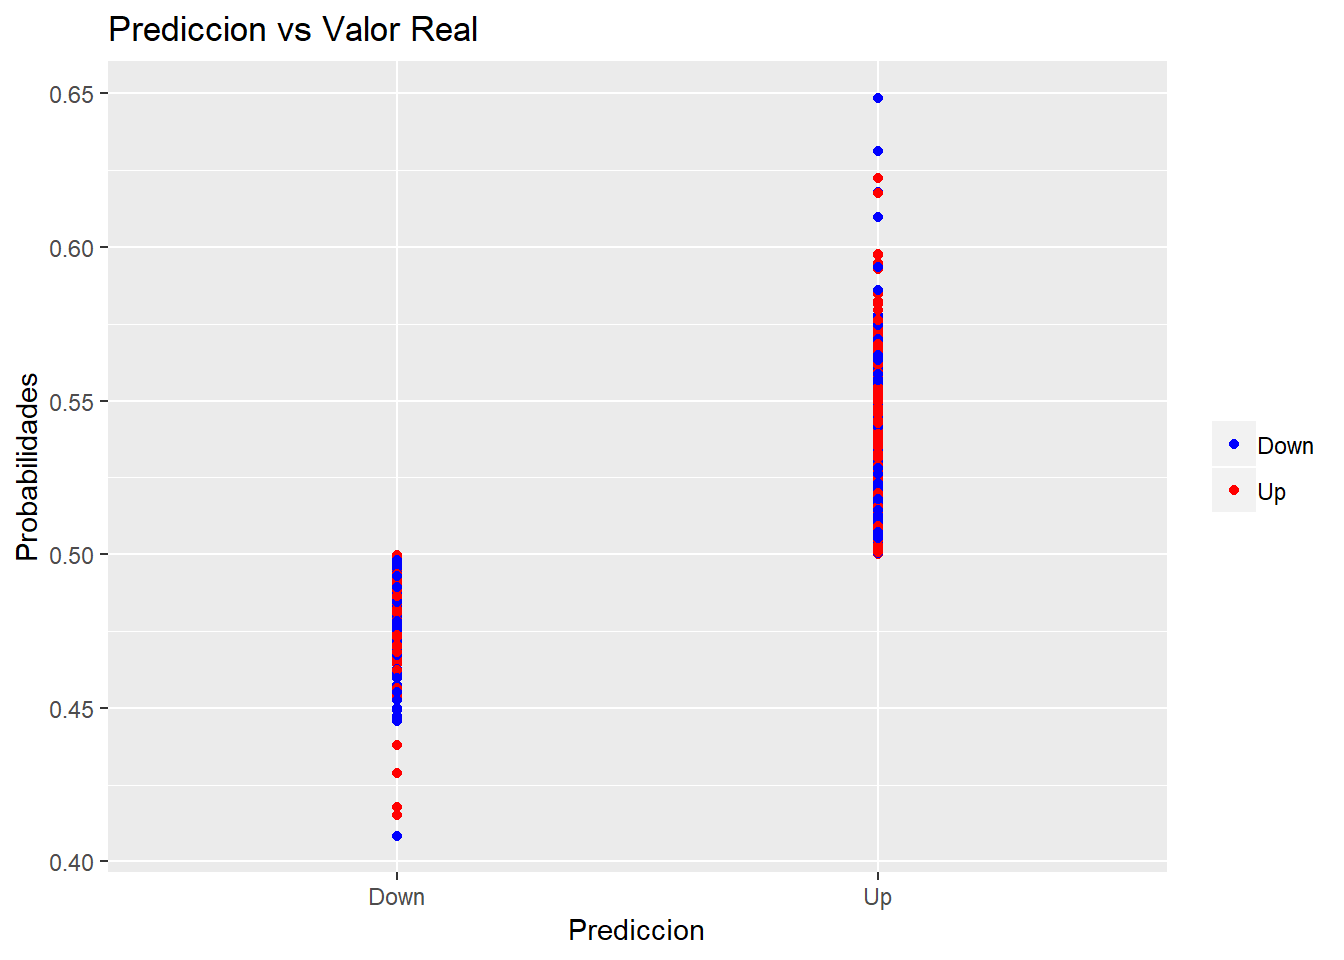
\includegraphics{04-RegresionLogistica_files/figure-latex/unnamed-chunk-14-1.pdf}

\hypertarget{otros-ejemplos}{%
\subsection{Otros ejemplos}\label{otros-ejemplos}}

\begin{itemize}
\item
  \href{https://www.r-bloggers.com/how-to-perform-a-logistic-regression-in-r/}{How to perform a Logistic Regression in R}
\item
  \href{https://stats.idre.ucla.edu/r/dae/logit-regression/}{Logit Regression \textbar{} R Data Analysis Examples}
\item
  \href{https://www.hackerearth.com/practice/machine-learning/machine-learning-algorithms/logistic-regression-analysis-r/tutorial/}{Practical Guide to Logistic Regression Analysis in R}
\item
  \href{http://www.treselle.com/blog/customer-churn-logistic-regression-with-r/}{Customer Churn -- Logistic Regression with R}
\end{itemize}

\hypertarget{series-temporales}{%
\chapter{Series Temporales}\label{series-temporales}}

\begin{quote}
Ejemplo A:
\end{quote}

\includegraphics{05-SeriesTemporales_files/figure-latex/unnamed-chunk-2-1.pdf}

\begin{quote}
Ejemplo B:
\end{quote}

\includegraphics{05-SeriesTemporales_files/figure-latex/unnamed-chunk-3-1.pdf}

Una \textbf{serie temporal} es una secuencia de datos, medidos a intervalos de tiempo sucesivos regularmente espaciados.

\textbf{Ejemplos} de series temporales son:

\begin{itemize}
\tightlist
\item
  tasa de cambio diario,
\item
  tasa de desempleo mensual,
\item
  PIB trimestral,
\item
  volumen de lluvia diario,
\item
  etc.
\end{itemize}

Una de las características más importantes de una serie temporal es que las observaciones vecinas son generalmente dependientes. Así, mientras que en los modelos de regresión, por ejemplo, el orden de las observaciones es irrelevante para el análisis, en las series temporales \textbf{el orden de los datos es crucial}.

\hypertarget{que-es-una-serie-temporal}{%
\section{¿Qué es una Serie Temporal?}\label{que-es-una-serie-temporal}}

Una \textbf{serie temporal} (o simplemente una serie) es una secuencia de \(N\) observaciones ordenadas y equidistantes cronológicamente sobre una característica o varias características de una unidad observable en diferentes momentos.

\begin{itemize}
\tightlist
\item
  Si la serie es sobre una característica se dice que es univariante o \textbf{escalar}.
\item
  Si la serie es sobre dos o más características se dice que es multivariante o \textbf{vectorial}.
\end{itemize}

El estudio de las series temporales permite:

\begin{itemize}
\tightlist
\item
  \textbf{entender} mejor el mecanismo de generación de los datos, que puede no ser claro inicialmente en una investigación y/o
\item
  hacer pronósticos sobre el futuro, es decir: \textbf{previsiones}.
\end{itemize}

Las previsiones se utilizan en forma constante en diversos campos: economía, finanzas, marketing, medio ambiente, ingeniería, etc. En general, las previsiones proporcionan una guía para las decisiones que deben tomarse.

Algunos ejemplos de uso de las previsiones son:

\begin{itemize}
\item
  En \textbf{Planeamiento y Control de Operaciones}. Las decisiones de producción de un artículo con base en los pronósticos de ventas. Es posible por ejemplo, detectar una disminución en la tendencia de ventas que conlleve a reducir la producción, o al contrario.
\item
  En Marketing. La decisión de invertir en publicidad puede depender de prever las ventas.
\item
  En \textbf{Economía}. Las decisiones del Banco de España, por ejemplo para el control de la inflación, requieren la previsión y el examen del comportamiento de ciertas variables macroeconómicas, como el PIB, la tasa de desempleo, el IPC, las tasas de inter?s a distintos plazos, activas y pasivas.
\item
  En \textbf{Turismo}. La previsión del de número de turistas mensuales para determinar la demanda hotelera.
\item
  En \textbf{Epidemiología} y \textbf{Medio Ambiente}. La vigilancia de los niveles de contaminantes en el aire tiene como herramienta fundamental las series de tiempo. Pero adicionalmente el efecto de estos niveles sobre la salud.
\end{itemize}

Todas las series temporales tienen características particulares. Asi por ejemplo, las series pueden:

\begin{itemize}
\tightlist
\item
  evolucionar alrededor de un \textbf{nivel} constante o tienen \textbf{tendencias} crecientes o decrecientes,
\item
  evolucionar alrededor de un nivel que cambia sin seguir aparentemente un patrón concreto - tienen tendencia estocástica -
\item
  presentar reducciones (en invierno) y aumentos (en verano) sistemáticos en su nivel cada 12 meses - son \textbf{estacionales} -
\item
  presentar variabilidad constante alrededor de su nivel
\item
  presentar variabilidad condicional o alta \textbf{volatilidad},
\item
  moverse conjuntamente con otras series - tendencia común -
\item
  etc.
\end{itemize}

\begin{quote}
Ejemplo: Caudal Anual del Río Nilo. 1871--1970. Anual.
\end{quote}

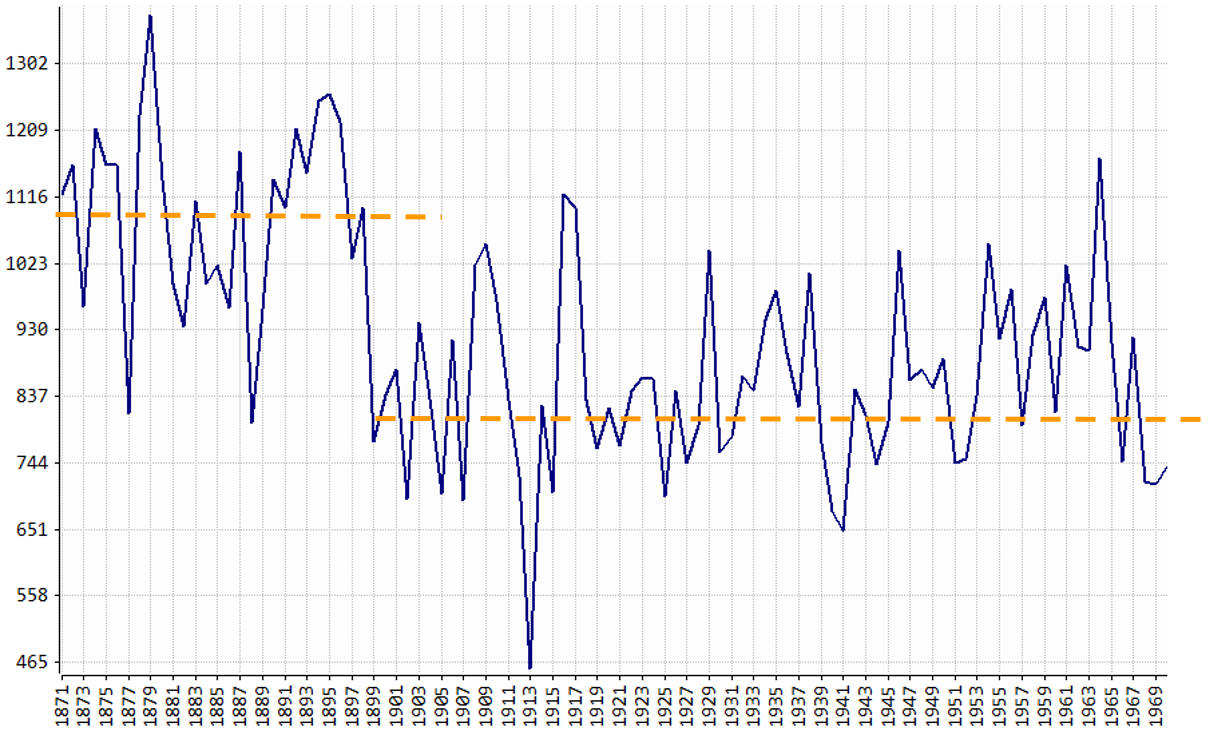
\includegraphics[width=0.9\linewidth]{C:/Users/romy.rodriguez/Documents/INNOVA/Formacion/MiCurso/ModelizacionR/imgs/ts_rionilo}

\begin{quote}
Ejemplo: España: Viviendas Iniciadas. Ene-1989/Jun-2012. Mensual. Miles de Viviendas
\end{quote}

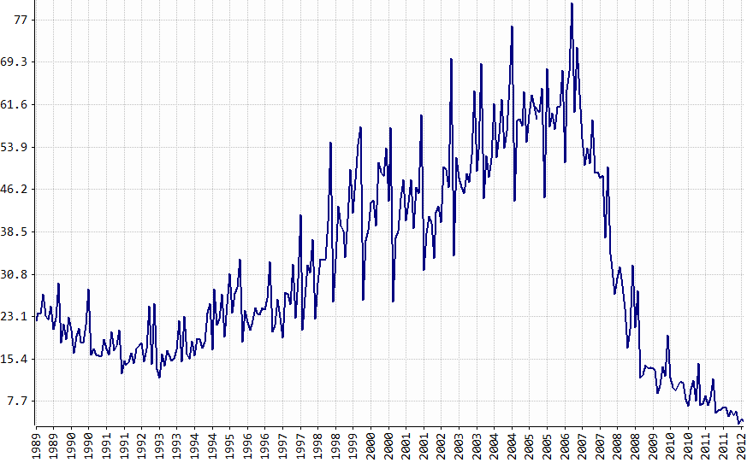
\includegraphics[width=0.9\linewidth]{C:/Users/romy.rodriguez/Documents/INNOVA/Formacion/MiCurso/ModelizacionR/imgs/ts_viviendas}

\begin{quote}
Ejemplo: Madrid: Temperatura Media en el Parque del Retiro. Ene-1989/Dic-2011. Mensual.
\end{quote}

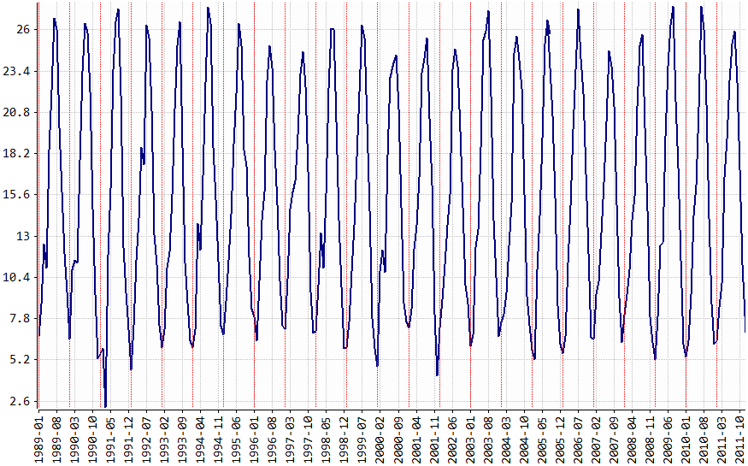
\includegraphics[width=0.9\linewidth]{C:/Users/romy.rodriguez/Documents/INNOVA/Formacion/MiCurso/ModelizacionR/imgs/ts_temperatura}

En las secciones siguiente se describen brevemente algunos conceptos necesarios para la modelación básica de series temporales.

\hypertarget{herramientas-de-analisis}{%
\section{Herramientas de Análisis}\label{herramientas-de-analisis}}

\hypertarget{autocorrelacion-acf-y-pacf}{%
\subsection{Autocorrelación (acf y pacf)}\label{autocorrelacion-acf-y-pacf}}

\begin{quote}
Los \textbf{correlogramas} permiten representar las funciones de autocorrelación simple (fas) y parcial (fap).
\end{quote}

El coeficiente de \textbf{correlación simple} (y así la fas) refleja la correlación entre la variable \(Y\) y el valor retardado de la misma en \(k\) instantes anteriores (\emph{lags}).

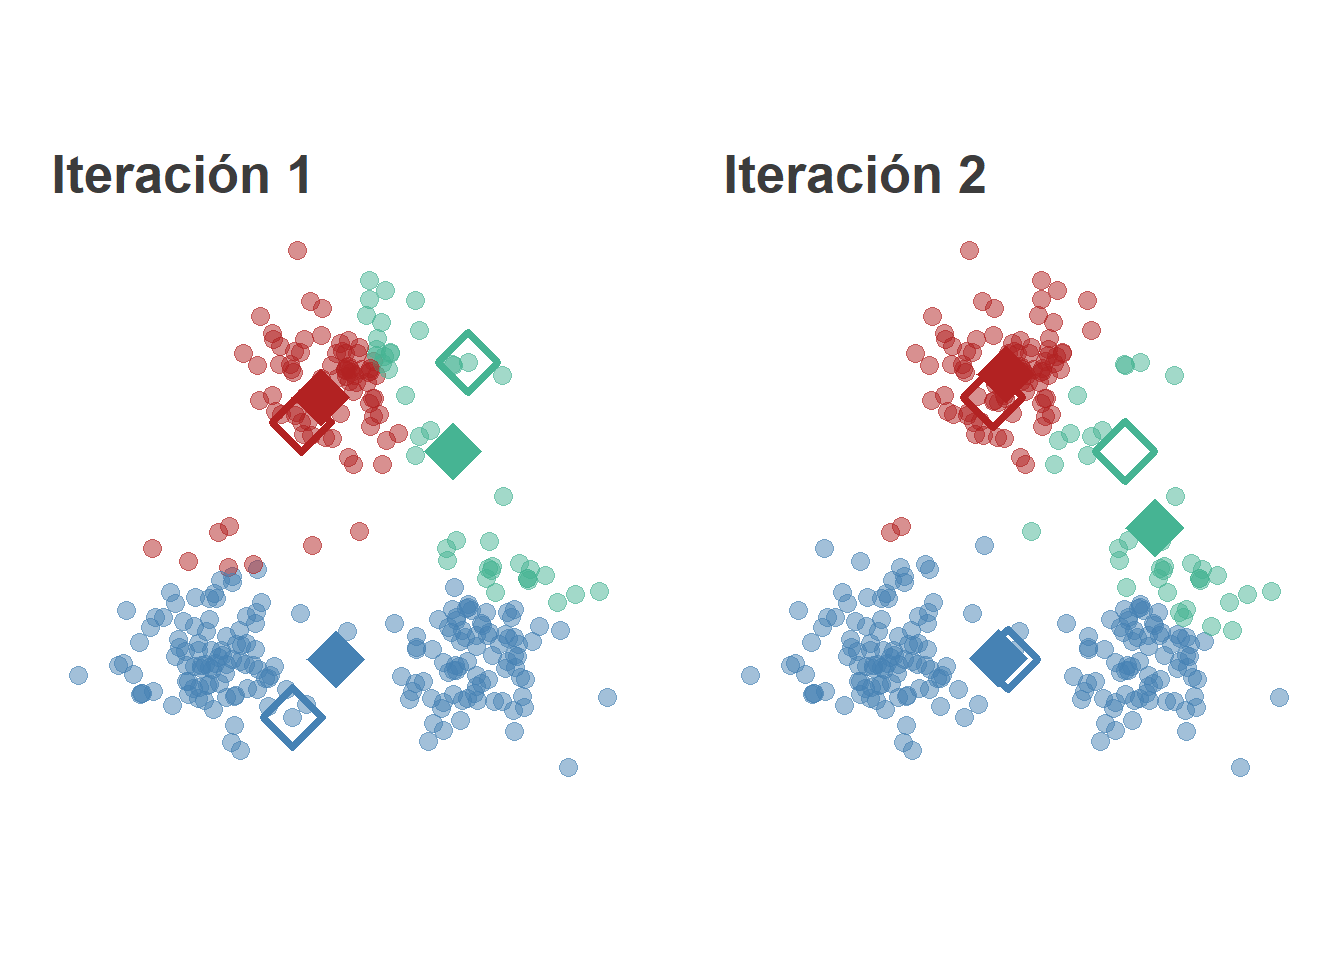
\includegraphics{05-SeriesTemporales_files/figure-latex/unnamed-chunk-7-1.pdf}

El **coeficiente de correlación parcial (y así la fap) calcula la correlación directa eliminando posibles dependencias asociadas a retardos intermedios.

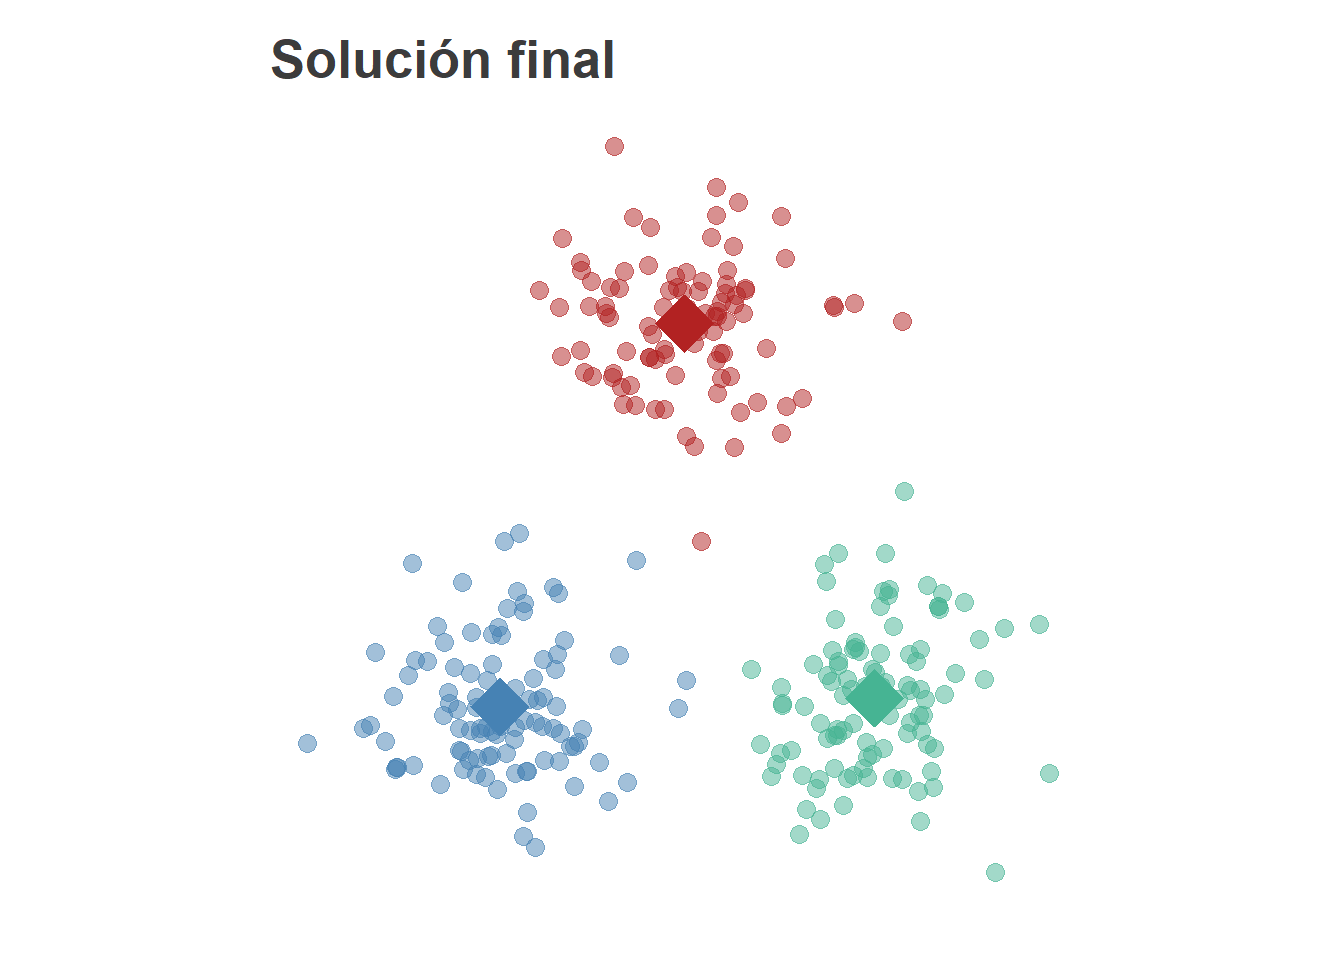
\includegraphics{05-SeriesTemporales_files/figure-latex/unnamed-chunk-8-1.pdf}

Los correlogramas permiten representar las \emph{acf} y \emph{pacf} que solo tienen sentido dentro del ámbito de los procesos estacionarios porque asumen que \textbf{la correlación entre dos valores de la serie sólo depende de su distancia}, no del instante del tiempo al que van referidos.

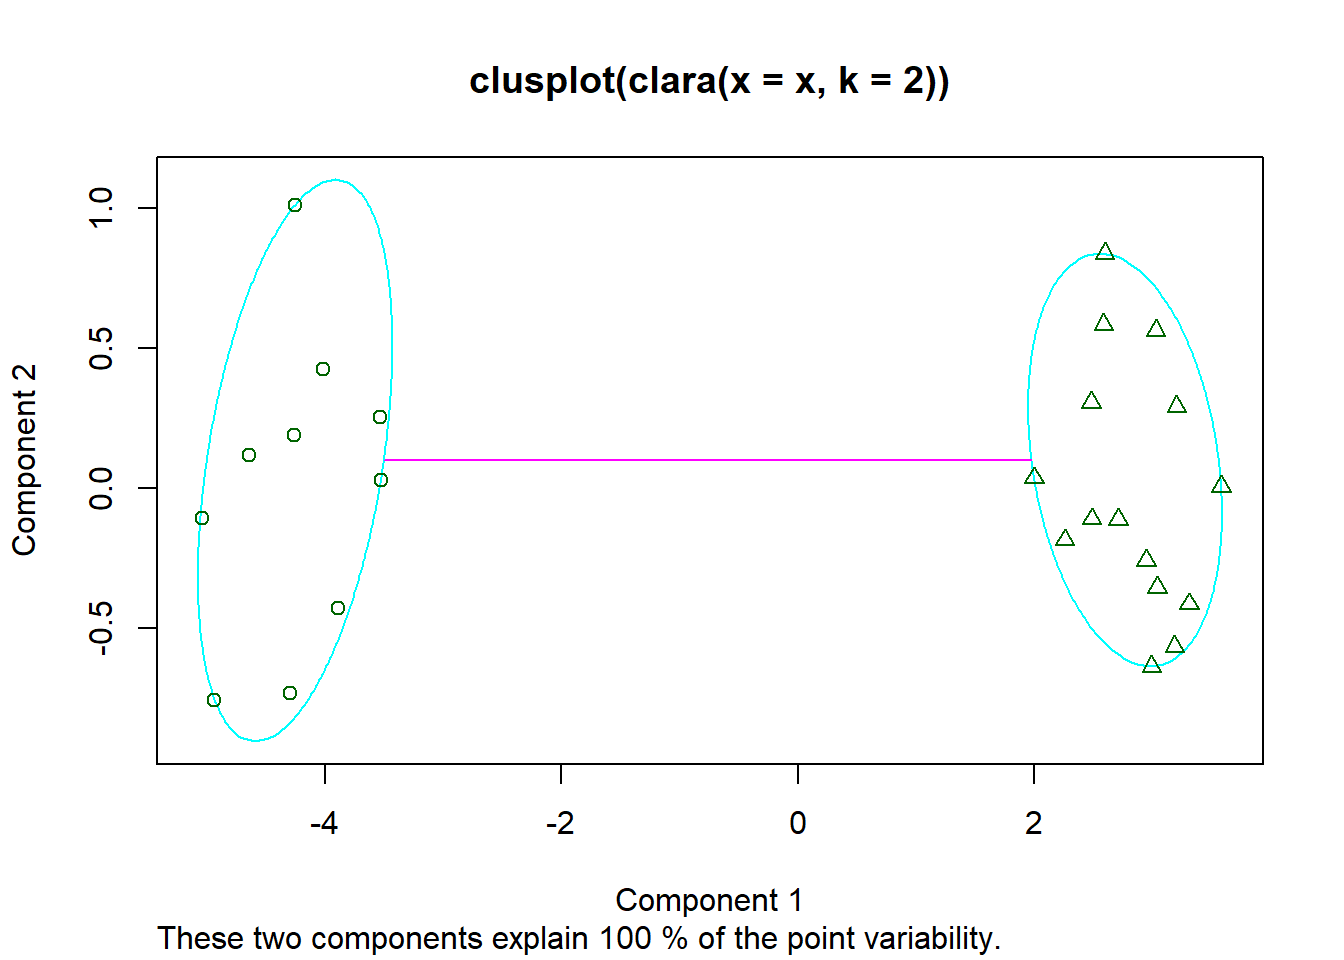
\includegraphics{05-SeriesTemporales_files/figure-latex/unnamed-chunk-9-1.pdf}

\hypertarget{operadores-del-tiempo}{%
\subsection{Operadores (del Tiempo)}\label{operadores-del-tiempo}}

\begin{quote}
Operador de \textbf{Retardo} Simple
\end{quote}

El \textbf{operador de retardo simple} se define como
\[Bz_t=z_{t-1}\]

Si aplicamos el operador de retardo dos veces:
\[BBz_t=Bz_{t-1}=z_{t-2}\]
Del mismo modo, si aplicamos \(n\) veces el operador de retardo, obtenemos:
\[ BB \ldots Bz_t=z_{t-n} \]
Definimos, por tanto
\[ B^n z_t=z_{t-n} \]

\begin{quote}
Operador de \textbf{Adelanto} simple
\end{quote}

De modo análogo, definimos el \textbf{operador de adelanto simple}
\[
\begin{align}
    Fz_t&=z_{t+1}\\
    F^n z_t&=z_{t+n}
\end{align}
\]

El operador \(F\) es el inverso del operador \(B\) ya que:
\[
FBz_t=BFz_t=z_t
\]
Por tanto, \(BF=FB=1,\) lo que implica que \(F=B^{-1}\).

\begin{quote}
Polinomios en \(B\)
\end{quote}

Sea el polinomio en el operador de retardo \(B\):
\[
\phi_0 - \phi_1 B - \ldots - \phi_pB^p
\]
La operación de este polinomio se define como:
\[
(\phi_0 - \phi_1 B - \ldots - \phi_pB^p)z_t=\phi_0z_t+\phi_1z_{t-1}+\ldots+\phi_pz_{t-p}
\]
Llamamos \textbf{polinomio autorregresivo} de orden \(p\) al polinomio de grado \(p\)
\[
1-\phi_1B-\dots-\phi_pB^p
\]
La razón de esta nomenclatura es que si tenemos una serie cuyo comportamiento puede expresarse como
\[
(1-\phi_1B-\dots-\phi_pB^p)z_t=e_t
\]
donde \(e_t\) es un término de error, la anterior expresión puede escribirse como:
\[
    z_t=\phi_1 z_{t-1}+ \ldots + \phi_p z_{t-p} + e_t
\]

Es decir, como una regresión donde la serie \(z_t\) es el \emph{output} y los propios retardos \(1,2,\ldots,p\) de la variable actúan como \emph{inputs} o regresores construyendo una \textbf{autorregresión}.

En muchas ocasiones emplearemos las formas \(\phi(B), \psi(B), \varphi(B)\) u otras semejantes para denotar polinomios en \(B\). Notaremos más adelante que asociaremos ciertas formas de expresar polinomios en \(B\) como \(\phi(B)\) a clases de polinomios en \(B\) que juegan cierto papel especial. Por ejemplo, reservaremos la expresi?n \(\phi(B)\) a polinomios autorregresivos.

\begin{quote}
Operador \textbf{Diferencia}
\end{quote}

El operador diferencia respecto al pasado, en lo sucesivo simplemente \textbf{operador diferencia}, se define como:
\[
\bigtriangledown z_t = z_t - z_{t-1},
\]
que puede expresarse como:
\[
\bigtriangledown z_t = z_t - z_{t-1},
\]
que puede expresarse como
\[
(1-B)z_t=\bigtriangledown z_t.
\]
Por lo tanto: \(\bigtriangledown =1-B\).
El operador de \textbf{diferencia peri?dica}, usualmente \textbf{diferencia estacional}, se define como
\[
\bigtriangledown_s z_t=z_t-z_{t-s}=(1-B^s)z_t.
\]
Luego, \(\bigtriangledown_s=(1-B^s).\)

Debe observarse que cuando aplicamos el operador \(B\) a una serie \(S\) lo que hacemos en realidad es \textbf{adelantar} la serie un periodo. Análogamente, cuando aplicamos el operador \(F\) a una serie \(S\) \textbf{retrasamos} la serie un periodo.

\hypertarget{alisado-exponencial}{%
\section{Alisado Exponencial}\label{alisado-exponencial}}

El alisado exponencial es una técnica aplicada a series de tiempo, para \textbf{suavizarlas} u obtener previsiones.

\begin{itemize}
\item
  Mientras que, con la media móvil, las observaciones pasadas se ponderan por igual, en el alisado exponencial se asignan ponderaciones exponencialmente decrecientes en el tiempo.
\item
  La fórmula utilizada es:

  \[ y_1 = x_0  \]
  \[ y_t = (1-\theta)x_{t-1}+\theta y_{t-1},  t > 1 \]
\end{itemize}

donde \(\{x_t\}\) son las observaciones reales, \(\{y_t\}\) son las estimaciones y \(\theta\) es el factor de alisamiento, \(0 < \theta < 1\).

En otras palabras, con este método, la previsión para el periodo \(t\) (valor esperado) como la suma ponderada de todas la observaciones anteriores, dando mayor importancia a las observaciones más recientes que a las más antiguas. Como puede verse en:

\[ y_t = (1-\theta) x_{t-1} +\theta y_{t-1} \]
\[ y_t = (1-\theta)x_{t-1}+(1-\theta)\theta x_{t-2}+(1-\theta) \theta^2 y_{t-2} \]
\[ y_t = (1-\theta)[x_{t-1}+\theta x_{t-2}+\theta x_{t-3}+\theta x_{t-4}+ ...] + \theta^{t-1} x_0 \]
Así, los pesos asignados a las observaciones previas pertenecen a una proporción de la progresión geométrica: \(\{1, \theta, \theta^2, \theta^3, ..\}\).

\begin{itemize}
\tightlist
\item
  Por otro lado, si la ecuación arriba se expresa como:
\end{itemize}

\[
                y_t = x_{t-1} + \theta(y_{t-1} - x_{t-1}) ,  
\]

Se aprecia que \(y_t\) está formada por la suma de la observación en el periodo anterior (\(x_{t-1}\)) más una proporción (\(\theta\)) del error cometido (\(y_{t-1} - x_{t-1}\)). Por lo tanto el valor de \(\theta\) controla la rapidez con que la previsión se adapta a los cambios del nivel de la serie (estado).

\begin{itemize}
\tightlist
\item
  Si \(\theta\) es grande (próximo a 1), la previsión se adapta rápidamente a los cambios, por lo tanto se debe utilizar en series poco estables.
\item
  Si \(\theta\) es pequeño (próximo a 0), se consigue eliminar el efecto de las fluctuaciones, por lo tanto se debe utilizar en series estables.
\item
  El valor de \(\theta\) se puede optimizar minimizando la suma de cuadrados del error de previsión, es decir, resolviendo: \(min(x_{t-1} - y_{t-1})^2\).
\item
  El alisado exponencial, técnicamente, es equivalente a un modelo \emph{ARIMA (0,1,1)} sin constante. En otras palabras, se puede representar por:
\end{itemize}

\[\hat{y} = (1-\theta)(1 + \theta B + \theta^2 B^2 + \theta^3 B^3 + ...)x_{t-1}\]

donde \(B\) es el operador retardo y \(\theta\) es el parámetro de amortiguamiento. Esta representación no implica recargar el último término con un peso mayor a los valores más recientes.

Si existe un número finito de periodos observados, la ecuación anterior se reescribe como:

\[ \hat{y} = \alpha (1 + \theta B + \theta^2 B^2 + ... + \theta^p B^p)x_{t-1}\]
donde \(p\) es el número de periodos disponibles y \$\alpha \textless{}1 \$ es un término que asegura que los coeficientes de la ecuación sumen la unidad. Eso permite que el peso relativo de cada uno de los datos del pasado se mantenga constante y, al mismo tiempo, el resultado siga siendo una media.

\begin{itemize}
\tightlist
\item
  En la tabla abajo se muestran los pesos que toman los términos, en el caso de contar con 6.
\end{itemize}

\begin{longtable}[]{@{}lcrrrr@{}}
\toprule
& I & II & III & IV & V\tabularnewline
\midrule
\endhead
\(\theta\) & 0.70 & 0.65 & 0.60 & 0.55 & 0.50\tabularnewline
\((1- \theta)\) & 0.30 & 0.35 & 0.40 & 0.45 & 0.50\tabularnewline
\((1- \theta)\theta\) & 0.21 & 0.23 & 0.24 & 0.25 & 0.25\tabularnewline
\((1- \theta)\theta^2\) & 0.15 & 0.15 & 0.14 & 0.14 & 0.13\tabularnewline
\((1- \theta)\theta^3\) & 0.10 & 0.10 & 0.09 & 0.07 & 0.06\tabularnewline
\((1- \theta)\theta^4\) & 0.07 & 0.06 & 0.05 & 0.04 & 0.03\tabularnewline
\((1- \theta)\theta^5\) & 0.05 & 0.04 & 0.03 & 0.02 & 0.02\tabularnewline
\bottomrule
\end{longtable}

\hypertarget{arima}{%
\section{ARIMA}\label{arima}}

\begin{quote}
Un proceso estocástico es un mecanismo generador de un número aleatorio de series. Una serie temporal es una realización particular de un proceso estocástico.
\end{quote}

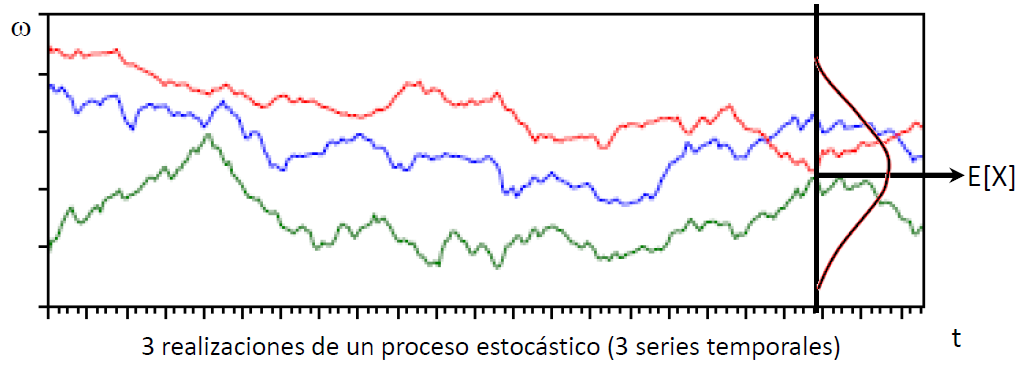
\includegraphics[width=0.9\linewidth]{C:/Users/romy.rodriguez/Documents/INNOVA/Formacion/MiCurso/ModelizacionR/imgs/ts_procesoEstocastico.png }

El objetivo que se plantea es \textbf{inferir el proceso estocástico que ha generado el conjunto de observaciones} que definen la serie temporal.

Para caracterizar un proceso estocástico \(F(y(t_1),\ldots,y(t_N))\), se requiere de la distribución conjunta de \(F(y_t), \forall t\), las distribuciones marginales \(F(y_t,y_{t+1}), \forall t\), etc.

\begin{itemize}
\item
  \textbf{Problema}. Como sólo se dispone de una observación por instante temporal, no es posible obtener dichas distribuciones.
\item
  \textbf{Solución}. Asumir qe las distribuiones son estables (estacionarias) en el tiempo para que las distribuciones asociadas a diferentes instantes sean comparables.
\end{itemize}

\begin{quote}
Un proceso es \textbf{estacionario} en sentido estricto si el comportamiento de una colección de variables aleatórias sólo depende de su posición relativa, no del instante \(t\).
\end{quote}

Dada una serie temporal, el objetivo es hacerla estacionaria para asumir esa estabilidad que permita hacer que todos los instantes sean comparables.

Una vez que el proceso (serie) es estacionario, se busca algún tipo de modelo adecuado para su caracterización: \textbf{los procesos ARMA son modelizables mediante modelos ARMA}.

\[ARMA(p,q) = (1-\phi_1 B - \ldots - \phi_p B^p)X_t = (1- \theta_1 B - \ldots - \theta_q B^q)a_t\]

\hypertarget{parte-ar-autorregresiva}{%
\subsection{Parte AR (Autorregresiva)}\label{parte-ar-autorregresiva}}

\begin{quote}
La parte autogresica del modelos muestra la dependencia del dato real con su propio pasado. Se trata de una regresión de la variable en sí misma (autoregresión).
\end{quote}

\[AR(p): X_t= \mu_t + \phi_1X_{t-1} + \ldots + \phi_1X_{t-p} + a_t\]

\hypertarget{parte-ma-medias-moviles}{%
\subsection{Parte MA (Medias Móviles)}\label{parte-ma-medias-moviles}}

\begin{quote}
La parte de medias moviles muestra la dependencia del dato real con el pasado del proceso de error (media móvil de la serie de los errores)
\end{quote}

Los procesos \(MA\) siempre son estacionarios.

\[MA(q): X_t= \mu - \theta_1 a_{t-1} - \ldots - \theta_q a_{t-q} + a_t\]

Se requiere identificar el proceso que buyace bajo los datos, lo cual consiste en \textbf{identicar los órdenes} \(p\) y \(q\) del modelo ARMA que generó la serie temporal.

Las herramientas para identificar esos procesos son las funciones de autocorrelación simple y parcial.

\begin{quote}
Ejemplo AR(2): \(Y_t = 0.6Y_{t-1}+0.2Y_{t-2}+A_t\)
\end{quote}

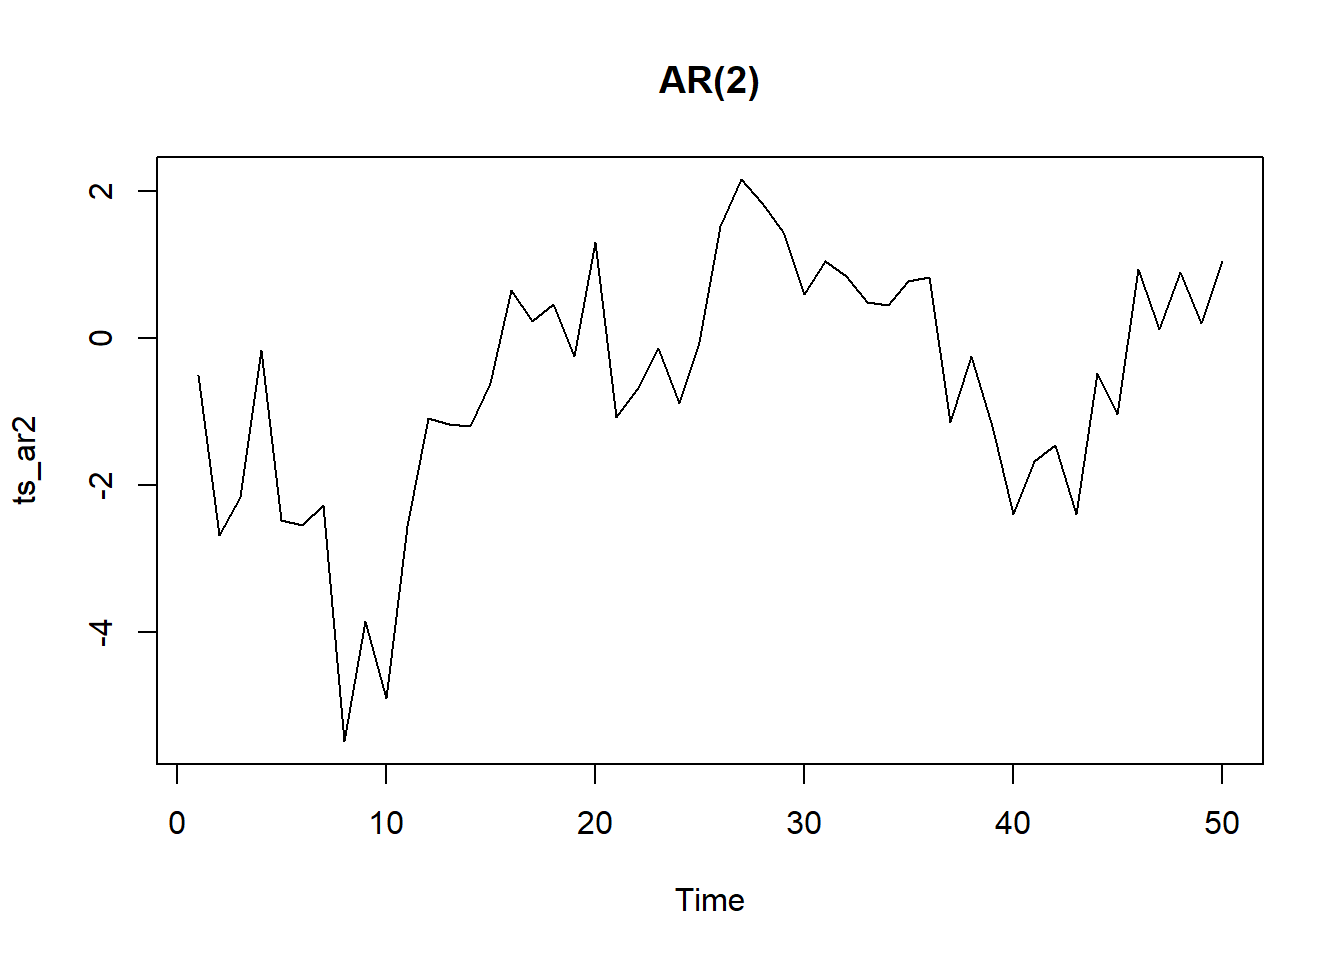
\includegraphics[width=0.95\linewidth]{05-SeriesTemporales_files/figure-latex/unnamed-chunk-11-1}
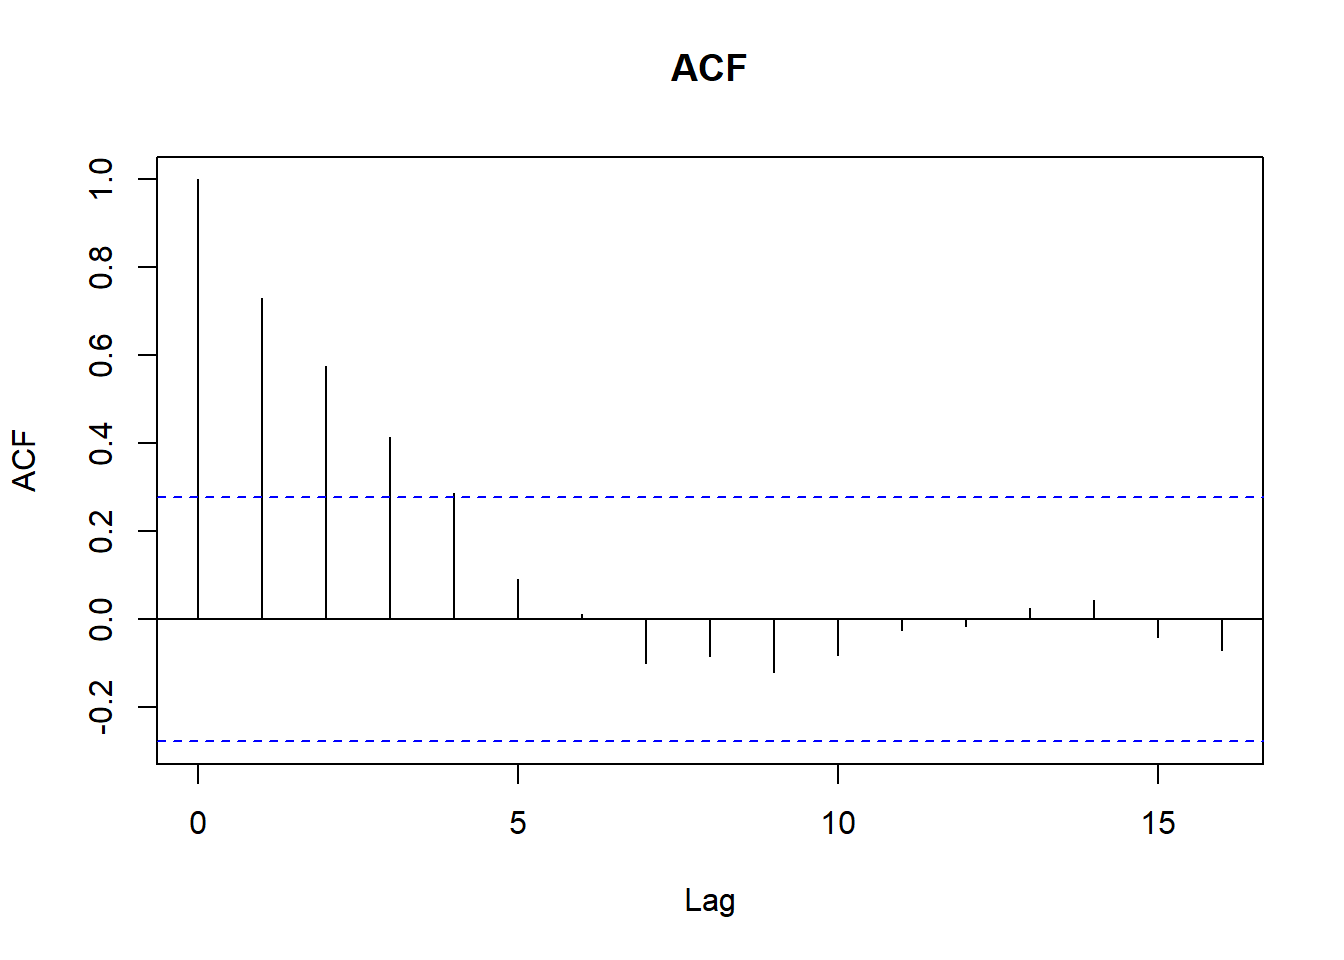
\includegraphics[width=0.95\linewidth]{05-SeriesTemporales_files/figure-latex/unnamed-chunk-11-2}
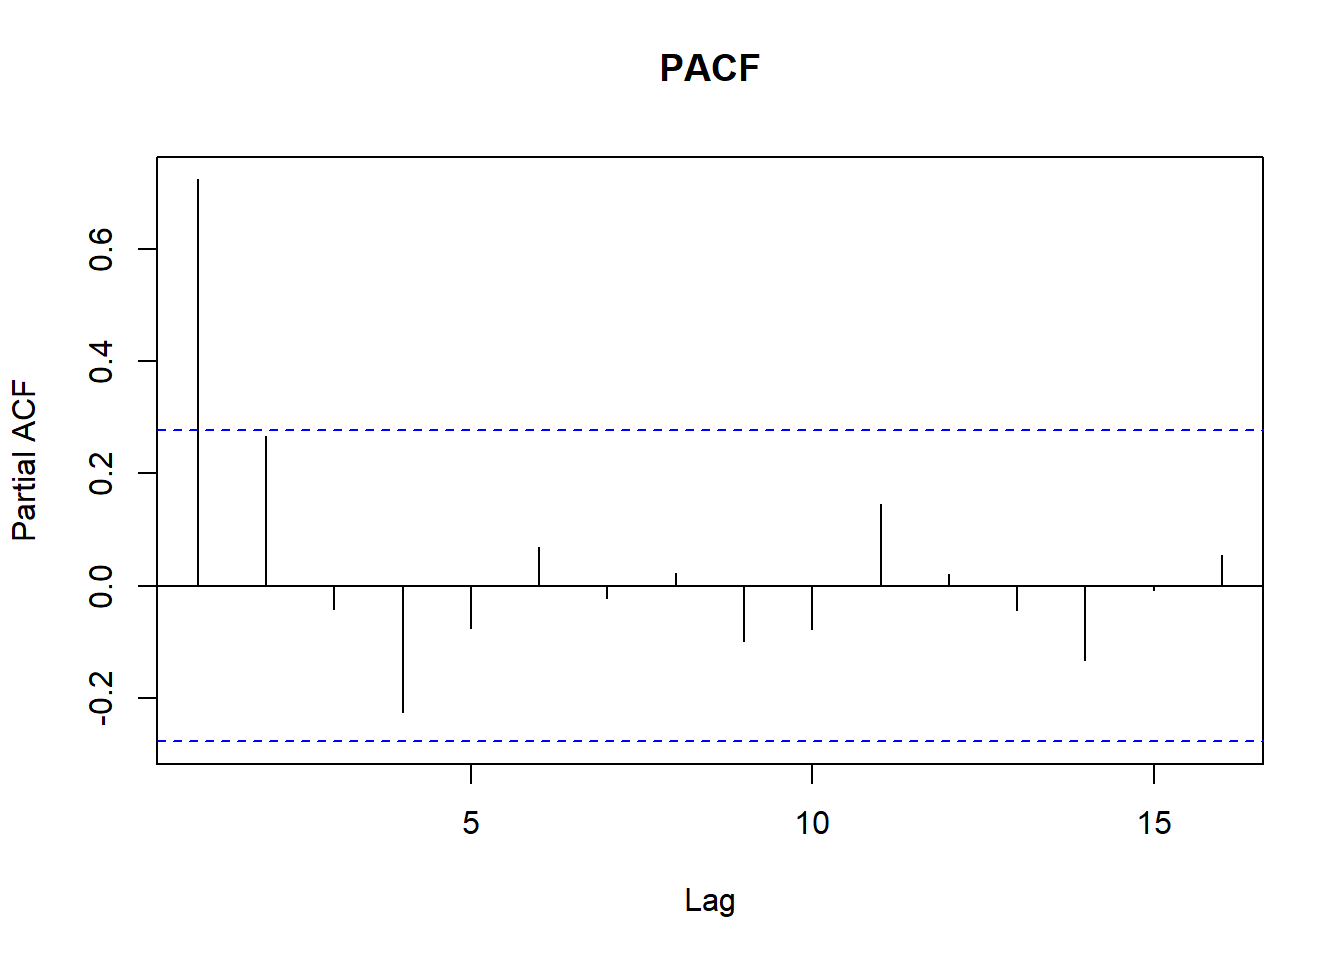
\includegraphics[width=0.95\linewidth]{05-SeriesTemporales_files/figure-latex/unnamed-chunk-11-3}

\begin{quote}
Ejemplo MA(2): \(X_t=A_t-0.6A_{t-1}-0.2A_{t-2}\)
\end{quote}

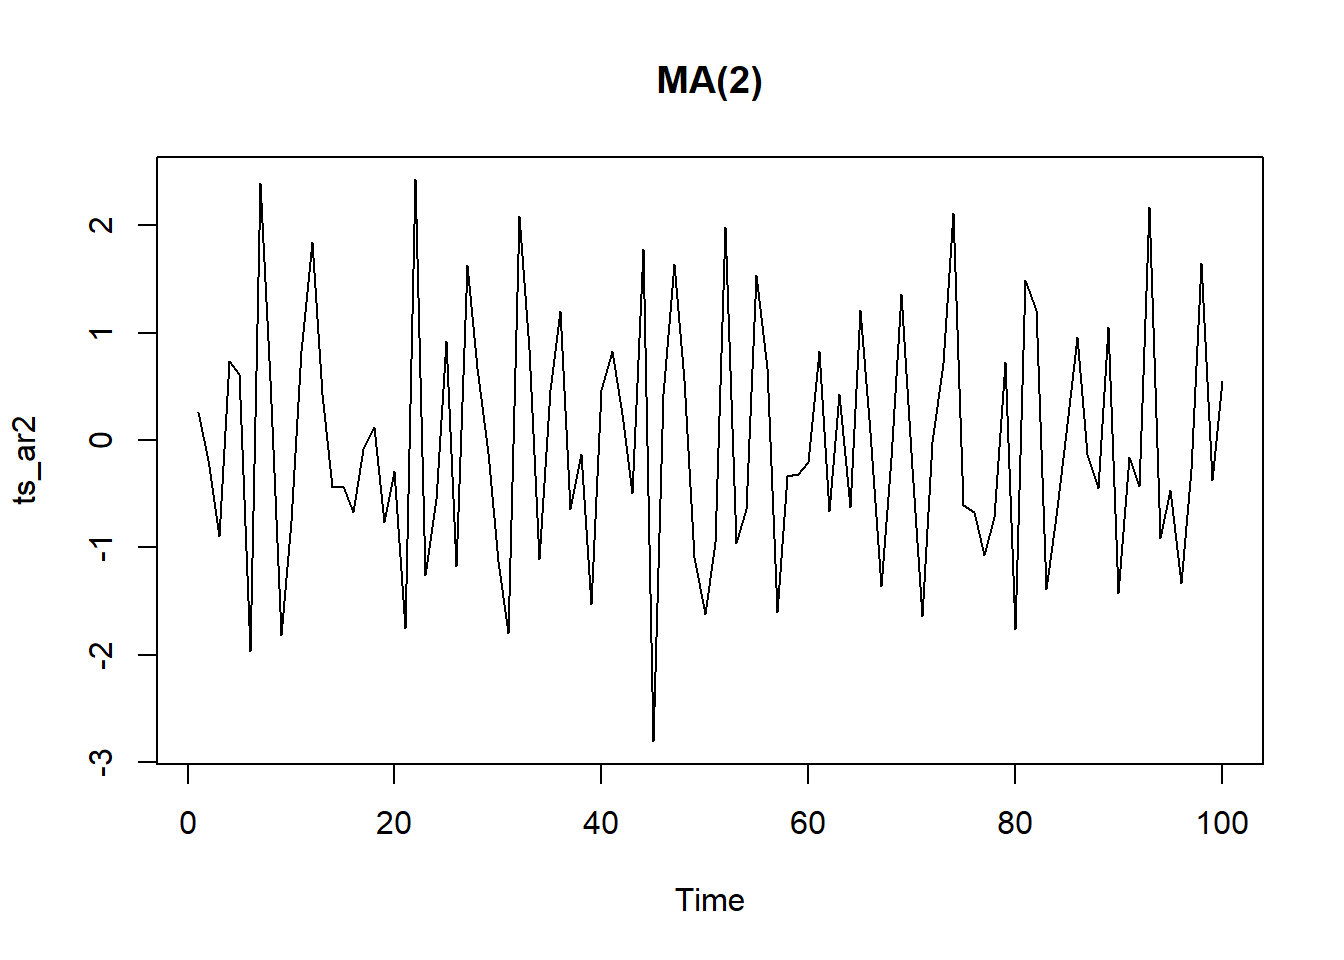
\includegraphics[width=0.95\linewidth]{05-SeriesTemporales_files/figure-latex/unnamed-chunk-12-1}
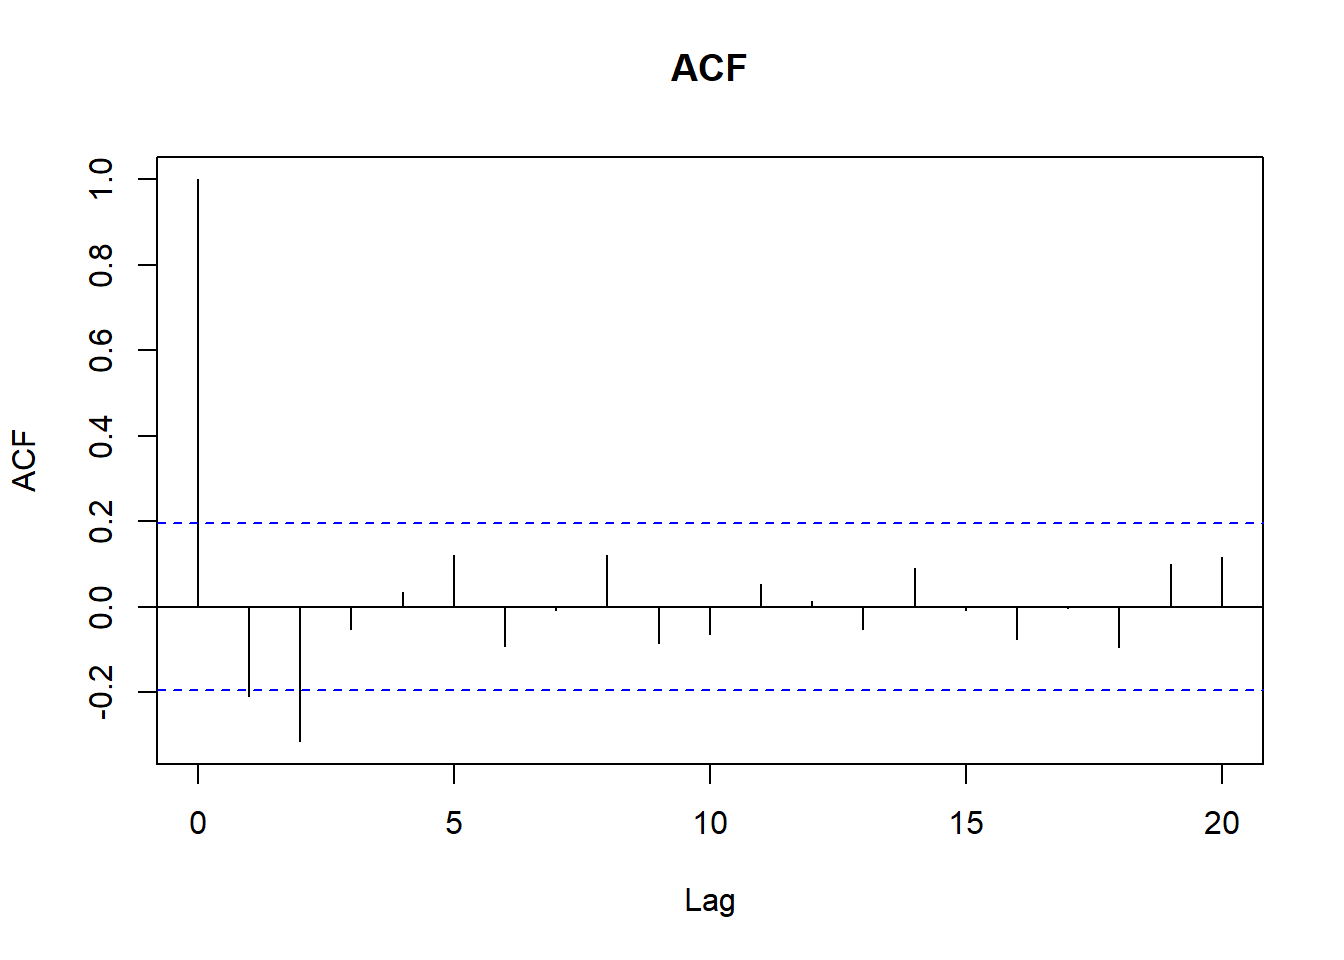
\includegraphics[width=0.95\linewidth]{05-SeriesTemporales_files/figure-latex/unnamed-chunk-12-2}
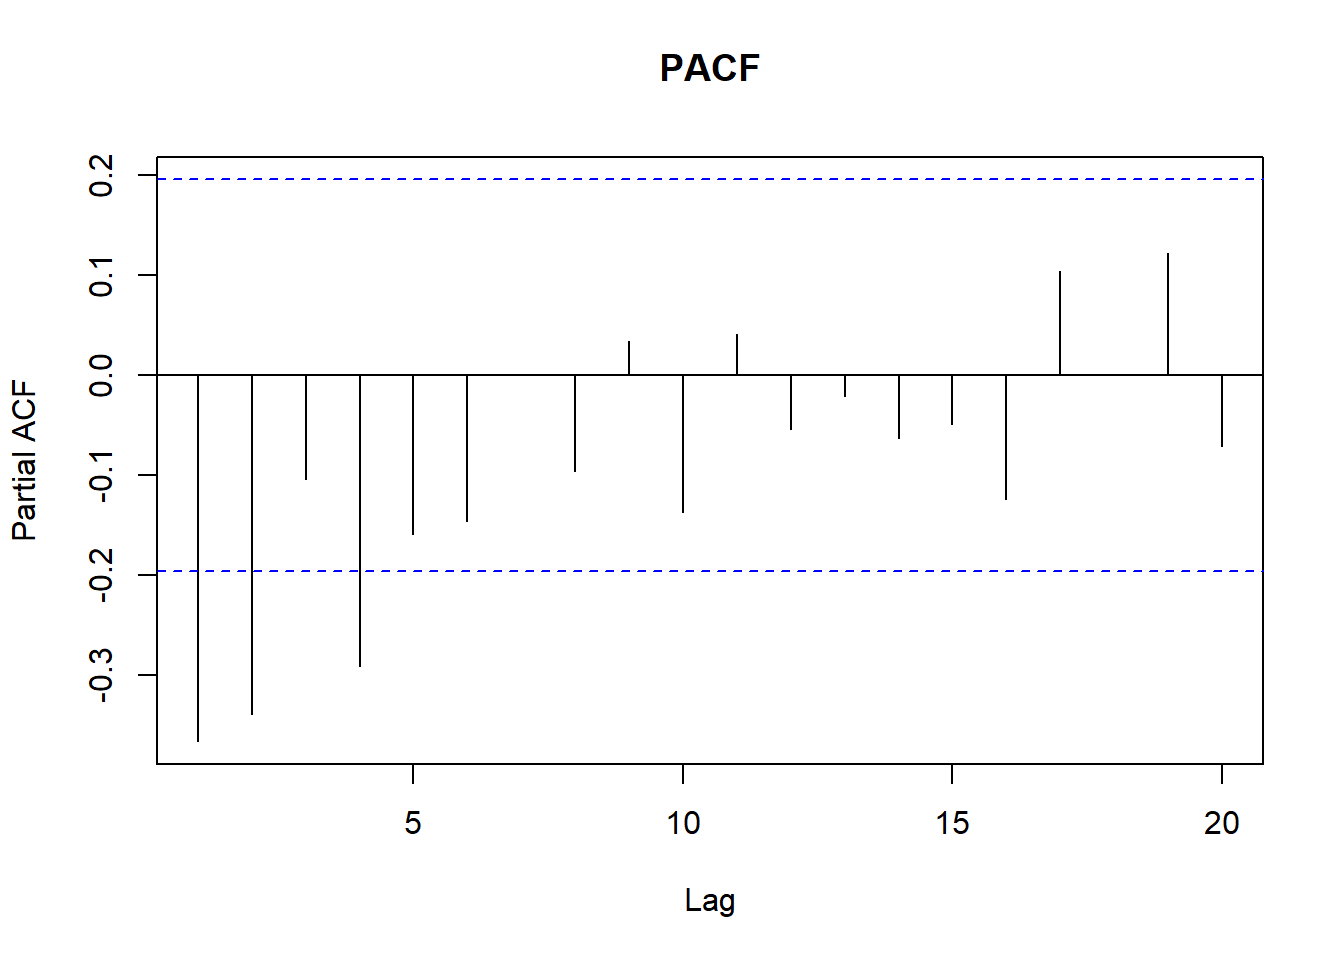
\includegraphics[width=0.95\linewidth]{05-SeriesTemporales_files/figure-latex/unnamed-chunk-12-3}

\begin{quote}
Ejemplo ARIMA(1,1):\(Y_t = -0.8 Y_{t-1} + A_t -0.8A_{t-1}\)
\end{quote}

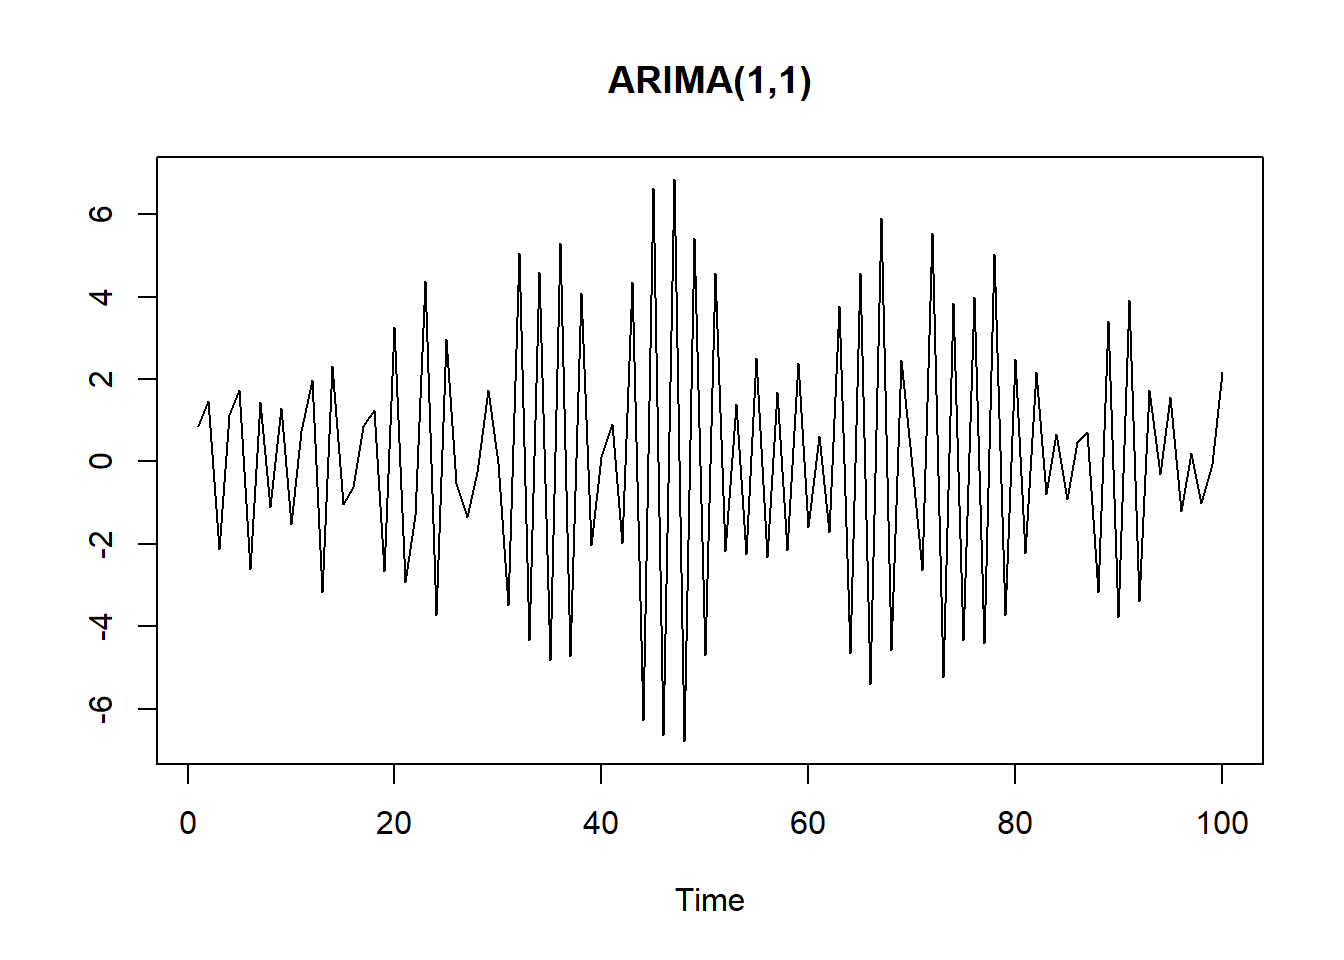
\includegraphics[width=0.9\linewidth]{05-SeriesTemporales_files/figure-latex/unnamed-chunk-13-1}
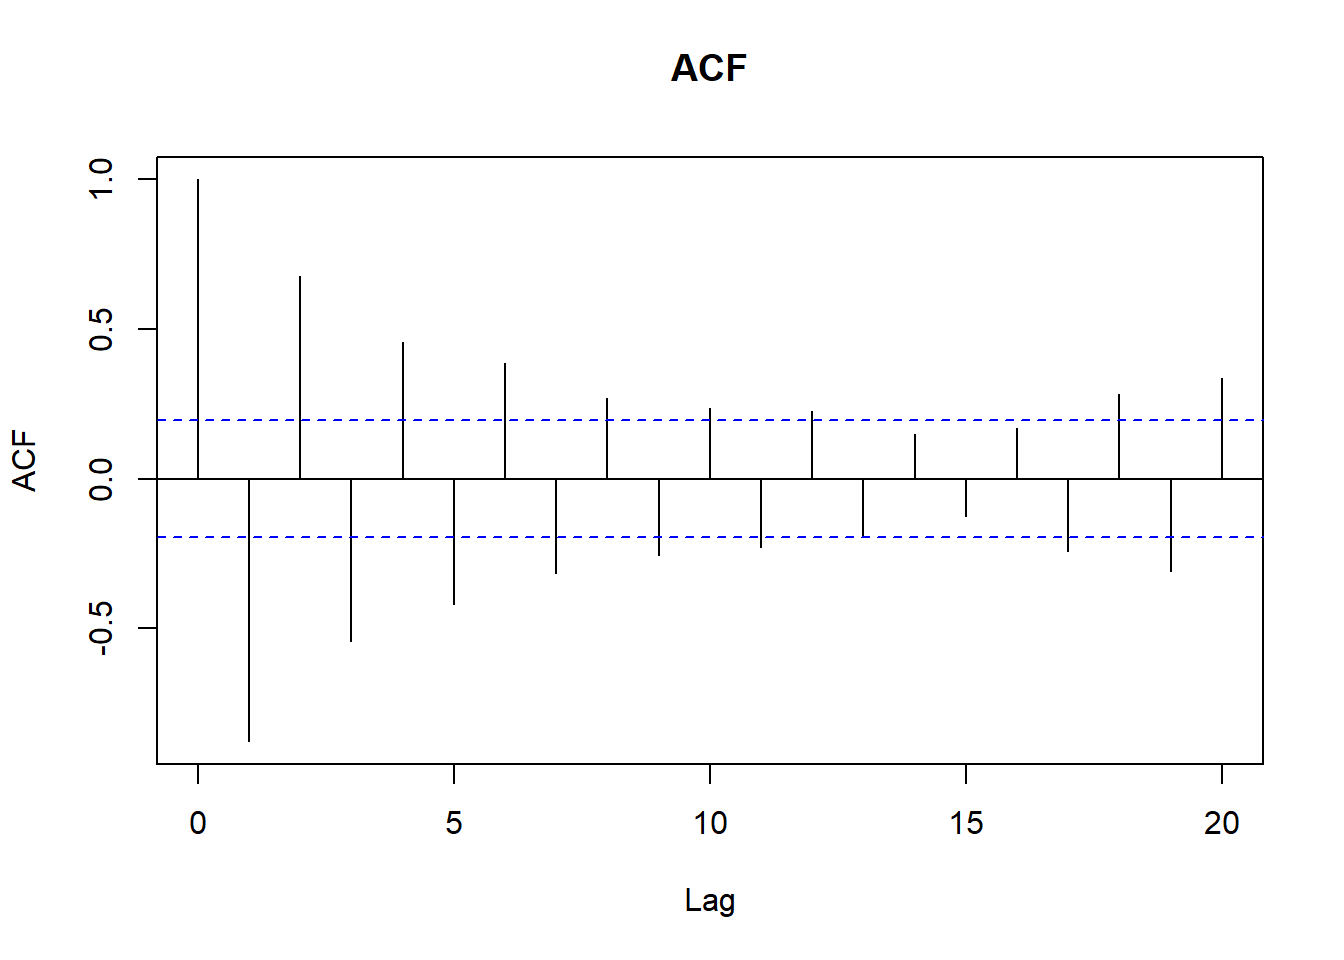
\includegraphics[width=0.9\linewidth]{05-SeriesTemporales_files/figure-latex/unnamed-chunk-13-2}

\hypertarget{funciones-de-transferencia}{%
\section{Funciones de Transferencia}\label{funciones-de-transferencia}}

Algunos ejemplos\footnote{Fuente de los gráficos}(\url{https://www.xycoon.com/tf_identification.htm}):

\includegraphics[width=0.9\linewidth]{C:/Users/romy.rodriguez/Documents/INNOVA/Formacion/MiCurso/ModelizacionR/imgs/tf_ide51}

\includegraphics[width=0.9\linewidth]{C:/Users/romy.rodriguez/Documents/INNOVA/Formacion/MiCurso/ModelizacionR/imgs/tf_ide52}

\includegraphics[width=0.9\linewidth]{C:/Users/romy.rodriguez/Documents/INNOVA/Formacion/MiCurso/ModelizacionR/imgs/tf_ide53}

\includegraphics[width=0.9\linewidth]{C:/Users/romy.rodriguez/Documents/INNOVA/Formacion/MiCurso/ModelizacionR/imgs/tf_ide54}

\includegraphics[width=0.9\linewidth]{C:/Users/romy.rodriguez/Documents/INNOVA/Formacion/MiCurso/ModelizacionR/imgs/tf_ide55}

\hypertarget{practica-en-r-3}{%
\section{Práctica en R}\label{practica-en-r-3}}

Un ejemplo sencillo sobre el manejo de series temporales que puede realizarse con algunos paquetes de R.

\begin{quote}
Datos
\end{quote}

Los datos utilizados corresponden a las \textbf{ventas mensuales} para una tienda de souvenirs en un balneario de Queensland, Australia, de enero de 1987 a diciembre de 1993 (Ver \href{http://robjhyndman.com/tsdldata/data/fancy.dat}{aquí}. Datos originales de Wheelwright y Hyndman, 1998).

\includegraphics{05-SeriesTemporales_files/figure-latex/unnamed-chunk-19-1.pdf}

\begin{quote}
Librerías
\end{quote}

A lo largo de esta práctica se utilizan las siguientes librerías:

\begin{itemize}
\tightlist
\item
  XTS: \emph{eXtensible Time Series} y
\item
  HIGHCHARTER: \emph{a R wrapper for Highcharts javascript libray and its modules. }.
\end{itemize}

Los manual de usuario de ambos paquetes esta disponibles en la siguientes enlaces: \href{http://cran.r-project.org/web/packages/xts/xts.pdf}{Manual de XTS} y \href{https://cran.r-project.org/web/packages/highcharter/highcharter.pdf}{Manual de HIGHCHARTER}

Para instalar un paquete de R, se puede usar el comando: \texttt{install.packages("nombre\ del\ paquete")}. Por ejemplo, \texttt{install.packages("xts")}. De forma alternativa:

\begin{Shaded}
\begin{Highlighting}[]
\CommentTok{# Get xts}
\ControlFlowTok{if}\NormalTok{ (}\OperatorTok{!}\KeywordTok{require}\NormalTok{(}\StringTok{"xts"}\NormalTok{)) \{}\KeywordTok{install.packages}\NormalTok{(}\StringTok{"xts"}\NormalTok{);    }\KeywordTok{library}\NormalTok{(xts)\}}
\CommentTok{# Get highcharter}
\ControlFlowTok{if}\NormalTok{ (}\OperatorTok{!}\KeywordTok{require}\NormalTok{(}\StringTok{"highcharter"}\NormalTok{)) \{}\KeywordTok{install.packages}\NormalTok{(}\StringTok{"highcharter"}\NormalTok{);    }\KeywordTok{library}\NormalTok{(highcharter)\}}
\CommentTok{# Get tseries}
\ControlFlowTok{if}\NormalTok{ (}\OperatorTok{!}\KeywordTok{require}\NormalTok{(}\StringTok{"tseries"}\NormalTok{)) \{}\KeywordTok{install.packages}\NormalTok{(}\StringTok{"tseries"}\NormalTok{);    }\KeywordTok{library}\NormalTok{(tseries)\}}
\end{Highlighting}
\end{Shaded}

\begin{quote}
Lectura y Visualización
\end{quote}

Obtenemos los datos en el site de la \emph{Time Series Data Library} (TSDL). (Los datos están \href{http://robjhyndman.com/tsdldata/data/fancy.dat}{aquí}.

\begin{Shaded}
\begin{Highlighting}[]
\NormalTok{datos =}\StringTok{ }\KeywordTok{scan}\NormalTok{(}\StringTok{"http://robjhyndman.com/tsdldata/data/fancy.dat"}\NormalTok{)}
\NormalTok{datos =}\StringTok{ }\KeywordTok{log}\NormalTok{(datos) }\CommentTok{#transformación opcional}

\KeywordTok{head}\NormalTok{(datos,}\DecValTok{5}\NormalTok{) }\CommentTok{#primeros 5 datos}
\end{Highlighting}
\end{Shaded}

\begin{verbatim}
FALSE [1] 7.41747 7.78219 7.95181 8.17394 8.23030
\end{verbatim}

\begin{Shaded}
\begin{Highlighting}[]
\KeywordTok{tail}\NormalTok{(datos,}\DecValTok{5}\NormalTok{) }\CommentTok{#últimos 5 datos}
\end{Highlighting}
\end{Shaded}

\begin{verbatim}
FALSE [1] 10.2607 10.3257 10.3360 10.7501 11.5585
\end{verbatim}

\begin{quote}
Objeto XTS
\end{quote}

La forma más conocida para la creación de un objeto de la clase serie temporal, es el uso de la función \texttt{ts}. En este ejemplo, creamos la serie temporal \texttt{sales.ts} a partir de \texttt{datos}.

Sin embargo, la manipulación de la serie es bastante más natural y amigable utilizando un objeto de la clase \texttt{xts}. En este ejemplo se crea el objeto \texttt{sales} a partir de \texttt{datos} y se hacen consultas básicas sobre su contenido (fechado, primer dato, últimas semanas, número de semanas en la muestra, etc.)

\begin{Shaded}
\begin{Highlighting}[]
\NormalTok{sales =}\StringTok{ }\KeywordTok{as.xts}\NormalTok{(sales.ts) }\CommentTok{#creación del objeto XTS}
\KeywordTok{is.xts}\NormalTok{(sales) }\CommentTok{#debe devolver TRUE}
\end{Highlighting}
\end{Shaded}

\begin{verbatim}
FALSE [1] TRUE
\end{verbatim}

\begin{Shaded}
\begin{Highlighting}[]
\KeywordTok{periodicity}\NormalTok{(sales) }\CommentTok{#fechado de los datos}
\end{Highlighting}
\end{Shaded}

\begin{verbatim}
FALSE Monthly periodicity from ene. 1987 to dic. 1993
\end{verbatim}

\begin{Shaded}
\begin{Highlighting}[]
\KeywordTok{first}\NormalTok{(sales) }\CommentTok{#primer dato}
\end{Highlighting}
\end{Shaded}

\begin{verbatim}
FALSE              [,1]
FALSE ene. 1987 7.41747
\end{verbatim}

\begin{Shaded}
\begin{Highlighting}[]
\KeywordTok{last}\NormalTok{(sales) }\CommentTok{#último dato}
\end{Highlighting}
\end{Shaded}

\begin{verbatim}
FALSE              [,1]
FALSE dic. 1993 11.5585
\end{verbatim}

\begin{Shaded}
\begin{Highlighting}[]
\KeywordTok{first}\NormalTok{(sales, }\StringTok{'7 months'}\NormalTok{) }\CommentTok{#primeros 7 dias}
\end{Highlighting}
\end{Shaded}

\begin{verbatim}
FALSE              [,1]
FALSE ene. 1987 7.41747
FALSE feb. 1987 7.78219
FALSE mar. 1987 7.95181
FALSE abr. 1987 8.17394
FALSE may. 1987 8.23030
FALSE jun. 1987 8.22006
FALSE jul. 1987 8.37784
\end{verbatim}

\begin{Shaded}
\begin{Highlighting}[]
\KeywordTok{last}\NormalTok{(sales, }\StringTok{'2 quarters'}\NormalTok{) }\CommentTok{#últimas dos semanas}
\end{Highlighting}
\end{Shaded}

\begin{verbatim}
FALSE              [,1]
FALSE jul. 1993 10.1718
FALSE ago. 1993 10.2607
FALSE sep. 1993 10.3257
FALSE oct. 1993 10.3360
FALSE nov. 1993 10.7501
FALSE dic. 1993 11.5585
\end{verbatim}

\begin{Shaded}
\begin{Highlighting}[]
\KeywordTok{nmonths}\NormalTok{(sales) }\CommentTok{#número de meses en la muestra}
\end{Highlighting}
\end{Shaded}

\begin{verbatim}
FALSE [1] 84
\end{verbatim}

\begin{Shaded}
\begin{Highlighting}[]
\KeywordTok{nquarters}\NormalTok{(sales) }\CommentTok{#número de trimestres en la muestra}
\end{Highlighting}
\end{Shaded}

\begin{verbatim}
FALSE [1] 28
\end{verbatim}

\begin{Shaded}
\begin{Highlighting}[]
\KeywordTok{nyears}\NormalTok{(sales) }\CommentTok{#número de años en la muestra}
\end{Highlighting}
\end{Shaded}

\begin{verbatim}
FALSE [1] 7
\end{verbatim}

\begin{quote}
Selección de datos usando las fechas
\end{quote}

Una funcionalidad interesante es la obtención de sub-muestras, utilizando la(s) fecha(s) como criterio(s) de selección.

\begin{Shaded}
\begin{Highlighting}[]
\NormalTok{sales[}\StringTok{'1990-01-01/1990-05-01'}\NormalTok{] }\CommentTok{#todos los datos del 01 al 05 de Febrero de 1990}
\end{Highlighting}
\end{Shaded}

\begin{verbatim}
FALSE              [,1]
FALSE ene. 1990 8.68628
FALSE feb. 1990 8.66812
FALSE mar. 1990 9.42716
FALSE abr. 1990 8.75932
FALSE may. 1990 8.93710
\end{verbatim}

\begin{Shaded}
\begin{Highlighting}[]
\KeywordTok{first}\NormalTok{(sales[}\StringTok{'1991'}\NormalTok{], }\StringTok{'5 month'}\NormalTok{) }\CommentTok{#primeros 5 meses desde Febrero de 1989}
\end{Highlighting}
\end{Shaded}

\begin{verbatim}
FALSE              [,1]
FALSE ene. 1991 8.48191
FALSE feb. 1991 8.77497
FALSE mar. 1991 9.17355
FALSE abr. 1991 9.08491
FALSE may. 1991 9.07365
\end{verbatim}

\begin{Shaded}
\begin{Highlighting}[]
\KeywordTok{last}\NormalTok{(sales[}\StringTok{'1990'}\NormalTok{], }\StringTok{'1 quarter'}\NormalTok{) }\CommentTok{#datos último mes de 1990}
\end{Highlighting}
\end{Shaded}

\begin{verbatim}
FALSE               [,1]
FALSE oct. 1990  9.04508
FALSE nov. 1990  9.79337
FALSE dic. 1990 10.31276
\end{verbatim}

\begin{Shaded}
\begin{Highlighting}[]
\KeywordTok{rbind}\NormalTok{(sales[}\StringTok{'1987-10/1988-03'}\NormalTok{],sales[}\StringTok{'1988-10/1989-03'}\NormalTok{]) }\CommentTok{#todos los datos del 01 al 05 de Febrero de 2011 y 2012}
\end{Highlighting}
\end{Shaded}

\begin{verbatim}
FALSE               [,1]
FALSE oct. 1987  8.76772
FALSE nov. 1987  8.93598
FALSE dic. 1987  9.89122
FALSE ene. 1988  7.82397
FALSE feb. 1988  8.55608
FALSE mar. 1988  8.88532
FALSE oct. 1988  8.67165
FALSE nov. 1988  9.44146
FALSE dic. 1988 10.25912
FALSE ene. 1989  8.45893
FALSE feb. 1989  8.64868
FALSE mar. 1989  9.20609
\end{verbatim}

\begin{quote}
Cambios de Fechado
\end{quote}

El cambio de fechado o periodicidad es una operación muy útil durante el trabajo con series temporales. En este ejemplo, como la variable analizada corresponde a las ventas mensuales, se utiliza la función \texttt{sum} para obtener las ventas trimestrales y anuales.

\begin{Shaded}
\begin{Highlighting}[]
\NormalTok{sales.qua=}\KeywordTok{apply.quarterly}\NormalTok{(sales, sum) }\CommentTok{# datos trimestrales}
 \KeywordTok{first}\NormalTok{(sales.qua, }\StringTok{'3 quarters'}\NormalTok{)}
\end{Highlighting}
\end{Shaded}

\begin{verbatim}
FALSE              [,1]
FALSE mar. 1987 23.1515
FALSE jun. 1987 24.6243
FALSE sep. 1987 25.0787
\end{verbatim}

\begin{Shaded}
\begin{Highlighting}[]
\NormalTok{sales.yea=}\KeywordTok{apply.yearly}\NormalTok{(sales, sum) }\CommentTok{# datos anuales}
 \KeywordTok{first}\NormalTok{(sales.yea, }\StringTok{'3 years'}\NormalTok{)}
\end{Highlighting}
\end{Shaded}

\begin{verbatim}
FALSE              [,1]
FALSE dic. 1987 100.449
FALSE dic. 1988 105.113
FALSE dic. 1989 108.676
\end{verbatim}

\begin{quote}
Imputación de Datos Faltantes
\end{quote}

La falta de algunos datos y/o la presencia de datos errones suele tratarse con procedimientos de imputación - para no perder histórico de la muestra disponible. El paquete \texttt{xts} posee funciones que permiten extender hacia adelante o hacia atrás, valores observados en la misma serie temporal.

\begin{Shaded}
\begin{Highlighting}[]
\NormalTok{aux=sales[}\StringTok{'1990-01-01/1990-03-01'}\NormalTok{]}
\NormalTok{sales[}\StringTok{'1990-01-01/1990-03-01'}\NormalTok{]=}\OtherTok{NA}
\NormalTok{sales[}\StringTok{'1990-01-01/1990-03-01'}\NormalTok{]}
\end{Highlighting}
\end{Shaded}

\begin{verbatim}
FALSE           [,1]
FALSE ene. 1990   NA
FALSE feb. 1990   NA
FALSE mar. 1990   NA
\end{verbatim}

\begin{Shaded}
\begin{Highlighting}[]
\NormalTok{(}\DataTypeTok{isna=}\KeywordTok{which}\NormalTok{(}\KeywordTok{is.na}\NormalTok{(sales))) }\CommentTok{#identifica las líneas con NA}
\end{Highlighting}
\end{Shaded}

\begin{verbatim}
FALSE [1] 37 38 39
\end{verbatim}

\begin{Shaded}
\begin{Highlighting}[]
\NormalTok{sales.na01=}\KeywordTok{na.locf}\NormalTok{(sales) }\CommentTok{#repite el ultimo anterior a NA}
\NormalTok{ sales.na01[isna,]}
\end{Highlighting}
\end{Shaded}

\begin{verbatim}
FALSE              [,1]
FALSE ene. 1990 10.4359
FALSE feb. 1990 10.4359
FALSE mar. 1990 10.4359
\end{verbatim}

\begin{Shaded}
\begin{Highlighting}[]
\NormalTok{sales.na02=}\KeywordTok{na.locf}\NormalTok{(sales, }\DataTypeTok{fromLast=}\OtherTok{TRUE}\NormalTok{) }\CommentTok{# repite el primero despues de NA}
\NormalTok{ sales.na02[isna,]}
\end{Highlighting}
\end{Shaded}

\begin{verbatim}
FALSE              [,1]
FALSE ene. 1990 8.75932
FALSE feb. 1990 8.75932
FALSE mar. 1990 8.75932
\end{verbatim}

\begin{Shaded}
\begin{Highlighting}[]
\NormalTok{sales.na03=}\KeywordTok{na.locf}\NormalTok{(sales, }\DataTypeTok{na.rm=}\OtherTok{TRUE}\NormalTok{, }\DataTypeTok{fromLast=}\OtherTok{TRUE}\NormalTok{)}
\NormalTok{ sales.na03[isna,]}
\end{Highlighting}
\end{Shaded}

\begin{verbatim}
FALSE              [,1]
FALSE ene. 1990 8.75932
FALSE feb. 1990 8.75932
FALSE mar. 1990 8.75932
\end{verbatim}

\begin{Shaded}
\begin{Highlighting}[]
\NormalTok{sales[isna,]=aux}
\end{Highlighting}
\end{Shaded}

\begin{quote}
Estadísticos en diferentes fechados
\end{quote}

El paquete \texttt{xts}permite trabajar con series de estadísticos en fechado agregado. Por ejemplo, el máximo del mes, el mínimo del trimestre, etc. El ingrediente indispensable es el vector que indica los puntos de quiebre de la serie. Este vector se obtiene con la función \texttt{endpoints}.

\begin{Shaded}
\begin{Highlighting}[]
\NormalTok{aux.qq=}\KeywordTok{endpoints}\NormalTok{(sales,}\StringTok{"quarters"}\NormalTok{) }\CommentTok{#indica los finales de trimestre}
\KeywordTok{par}\NormalTok{(}\DataTypeTok{mfrow=}\KeywordTok{c}\NormalTok{(}\DecValTok{1}\NormalTok{,}\DecValTok{3}\NormalTok{), }\DataTypeTok{cex.lab=}\FloatTok{0.8}\NormalTok{,}\DataTypeTok{cex.axis=}\FloatTok{0.8}\NormalTok{,}\DataTypeTok{las=}\DecValTok{2}\NormalTok{)}
\KeywordTok{plot}\NormalTok{(}\KeywordTok{period.sum}\NormalTok{(sales,aux.qq), }\DataTypeTok{main=}\StringTok{"Total"}\NormalTok{) }
\KeywordTok{plot}\NormalTok{(}\KeywordTok{period.min}\NormalTok{(sales,aux.qq), }\DataTypeTok{main=}\StringTok{"Mínimo"}\NormalTok{)}
\KeywordTok{plot}\NormalTok{(}\KeywordTok{period.max}\NormalTok{(sales,aux.qq), }\DataTypeTok{main=}\StringTok{"Máximo"}\NormalTok{)}
\end{Highlighting}
\end{Shaded}

\includegraphics{05-SeriesTemporales_files/figure-latex/unnamed-chunk-27-1.pdf}

\begin{Shaded}
\begin{Highlighting}[]
\NormalTok{aux.yy=}\KeywordTok{endpoints}\NormalTok{(sales,}\StringTok{"years"}\NormalTok{) }\CommentTok{#indica los finales de año}
\KeywordTok{par}\NormalTok{(}\DataTypeTok{mfrow=}\KeywordTok{c}\NormalTok{(}\DecValTok{1}\NormalTok{,}\DecValTok{3}\NormalTok{),}\DataTypeTok{cex.lab=}\FloatTok{0.8}\NormalTok{,}\DataTypeTok{cex.axis=}\FloatTok{0.8}\NormalTok{,}\DataTypeTok{las=}\DecValTok{2}\NormalTok{)}
\KeywordTok{plot}\NormalTok{(}\KeywordTok{period.sum}\NormalTok{(sales,aux.yy), }\DataTypeTok{main=}\StringTok{"Total"}\NormalTok{)}
\KeywordTok{plot}\NormalTok{(}\KeywordTok{period.min}\NormalTok{(sales,aux.yy), }\DataTypeTok{main=}\StringTok{"Mínimo"}\NormalTok{)}
\KeywordTok{plot}\NormalTok{(}\KeywordTok{period.max}\NormalTok{(sales,aux.yy), }\DataTypeTok{main=}\StringTok{"Máximo"}\NormalTok{)}
\end{Highlighting}
\end{Shaded}

\includegraphics{05-SeriesTemporales_files/figure-latex/unnamed-chunk-27-2.pdf}

\begin{quote}
División del conjunto de datos usando fechas
\end{quote}

Otra funcionalidad útil es \texttt{split}. Permite dividir el objeto original en sub-conjuntos, teniendo en cuenta un fechado y un horizonte. En este caso, se divide el objeto \texttt{sales} en sub-muestras de 4 meses cada una.

\begin{Shaded}
\begin{Highlighting}[]
\NormalTok{sales.by}\FloatTok{.4}\NormalTok{months=}\KeywordTok{split}\NormalTok{(sales, }\DataTypeTok{f=}\StringTok{"months"}\NormalTok{,}\DataTypeTok{k=}\DecValTok{4}\NormalTok{) }
\NormalTok{sales.by}\FloatTok{.4}\NormalTok{months}
\end{Highlighting}
\end{Shaded}

\begin{verbatim}
## [[1]]
##              [,1]
## ene. 1987 7.41747
## feb. 1987 7.78219
## mar. 1987 7.95181
## abr. 1987 8.17394
## 
## [[2]]
##              [,1]
## may. 1987 8.23030
## jun. 1987 8.22006
## jul. 1987 8.37784
## ago. 1987 8.17930
## 
## [[3]]
##              [,1]
## sep. 1987 8.52155
## oct. 1987 8.76772
## nov. 1987 8.93598
## dic. 1987 9.89122
## 
## [[4]]
##              [,1]
## ene. 1988 7.82397
## feb. 1988 8.55608
## mar. 1988 8.88532
## abr. 1988 8.47763
## 
## [[5]]
##              [,1]
## may. 1988 8.68286
## jun. 1988 8.50741
## jul. 1988 8.72893
## ago. 1988 8.46635
## 
## [[6]]
##               [,1]
## sep. 1988  8.61185
## oct. 1988  8.67165
## nov. 1988  9.44146
## dic. 1988 10.25912
## 
## [[7]]
##              [,1]
## ene. 1989 8.45893
## feb. 1989 8.64868
## mar. 1989 9.20609
## abr. 1989 8.57636
## 
## [[8]]
##              [,1]
## may. 1989 8.77839
## jun. 1989 8.79948
## jul. 1989 8.90240
## ago. 1989 9.00903
## 
## [[9]]
##               [,1]
## sep. 1989  9.05639
## oct. 1989  9.17890
## nov. 1989  9.62588
## dic. 1989 10.43591
## 
## [[10]]
##              [,1]
## ene. 1990 8.68628
## feb. 1990 8.66812
## mar. 1990 9.42716
## abr. 1990 8.75932
## 
## [[11]]
##              [,1]
## may. 1990 8.93710
## jun. 1990 8.88527
## jul. 1990 9.00224
## ago. 1990 8.98460
## 
## [[12]]
##               [,1]
## sep. 1990  8.99876
## oct. 1990  9.04508
## nov. 1990  9.79337
## dic. 1990 10.31276
## 
## [[13]]
##              [,1]
## ene. 1991 8.48191
## feb. 1991 8.77497
## mar. 1991 9.17355
## abr. 1991 9.08491
## 
## [[14]]
##              [,1]
## may. 1991 9.07365
## jun. 1991 9.23107
## jul. 1991 9.33048
## ago. 1991 9.43765
## 
## [[15]]
##               [,1]
## sep. 1991  9.36198
## oct. 1991  9.51833
## nov. 1991  9.99068
## dic. 1991 10.71577
## 
## [[16]]
##              [,1]
## ene. 1992 8.93788
## feb. 1992 9.19520
## mar. 1992 9.58592
## abr. 1992 9.35767
## 
## [[17]]
##              [,1]
## may. 1992 9.14126
## jun. 1992 9.47900
## jul. 1992 9.72512
## ago. 1992 9.89790
## 
## [[18]]
##              [,1]
## sep. 1992 10.0830
## oct. 1992 10.1422
## nov. 1992 10.4920
## dic. 1992 11.2988
## 
## [[19]]
##              [,1]
## ene. 1993 9.23437
## feb. 1993 9.32962
## mar. 1993 9.99090
## abr. 1993 9.76177
## 
## [[20]]
##               [,1]
## may. 1993  9.68021
## jun. 1993  9.83100
## jul. 1993 10.17180
## ago. 1993 10.26069
## 
## [[21]]
##              [,1]
## sep. 1993 10.3257
## oct. 1993 10.3360
## nov. 1993 10.7501
## dic. 1993 11.5585
\end{verbatim}

\begin{Shaded}
\begin{Highlighting}[]
 \CommentTok{#divide el conjunto de datos en partes de 4 meses cada una}
\KeywordTok{summary}\NormalTok{(sales.by}\FloatTok{.4}\NormalTok{months) }\CommentTok{#indica el número de elemento que hay en cada parte}
\end{Highlighting}
\end{Shaded}

\begin{verbatim}
##       Length Class Mode   
##  [1,] 4      xts   numeric
##  [2,] 4      xts   numeric
##  [3,] 4      xts   numeric
##  [4,] 4      xts   numeric
##  [5,] 4      xts   numeric
##  [6,] 4      xts   numeric
##  [7,] 4      xts   numeric
##  [8,] 4      xts   numeric
##  [9,] 4      xts   numeric
## [10,] 4      xts   numeric
## [11,] 4      xts   numeric
## [12,] 4      xts   numeric
## [13,] 4      xts   numeric
## [14,] 4      xts   numeric
## [15,] 4      xts   numeric
## [16,] 4      xts   numeric
## [17,] 4      xts   numeric
## [18,] 4      xts   numeric
## [19,] 4      xts   numeric
## [20,] 4      xts   numeric
## [21,] 4      xts   numeric
\end{verbatim}

\begin{quote}
Otras operaciones con los datos
\end{quote}

Finalmente, se presenta un ejemplo de una serie obtenida a partir del uso de operaciones básicas de R como \texttt{diff} y \texttt{log}.

\begin{Shaded}
\begin{Highlighting}[]
\NormalTok{sales.inc <-}\StringTok{ }\KeywordTok{diff}\NormalTok{(}\KeywordTok{log}\NormalTok{(sales), }\DataTypeTok{lag =} \DecValTok{1}\NormalTok{) }\CommentTok{#Tasa de incremento mensual}
\NormalTok{sales.inc <-}\StringTok{ }\NormalTok{sales.inc[}\OperatorTok{-}\DecValTok{1}\NormalTok{] }\CommentTok{#Eliminamos el primer dato por ser NA}
\KeywordTok{par}\NormalTok{(}\DataTypeTok{mfrow=}\KeywordTok{c}\NormalTok{(}\DecValTok{1}\NormalTok{,}\DecValTok{1}\NormalTok{),}\DataTypeTok{cex.lab=}\FloatTok{0.8}\NormalTok{,}\DataTypeTok{cex.axis=}\FloatTok{0.8}\NormalTok{,}\DataTypeTok{las=}\DecValTok{2}\NormalTok{)}
\KeywordTok{plot}\NormalTok{(sales.inc, }\DataTypeTok{main =} \StringTok{"Nuevas Ventas"}\NormalTok{,}
     \DataTypeTok{col =} \StringTok{"grey"}\NormalTok{, }\DataTypeTok{xlab =} \StringTok{"Date"}\NormalTok{, }\DataTypeTok{ylab =} \StringTok{"Variación", major.ticks='years',}
\StringTok{     minor.ticks=FALSE)}
\end{Highlighting}
\end{Shaded}

\includegraphics{05-SeriesTemporales_files/figure-latex/unnamed-chunk-29-1.pdf}

\begin{quote}
Gráficos con xts
\end{quote}

Los gráficos de objetos \texttt{xts} son bastante más visuales o legibles que los objetos \texttt{ts}. La principal diferencia está en el reconocimiento de las fechas y su visualización en el eje horizontal.

\begin{Shaded}
\begin{Highlighting}[]
\KeywordTok{par}\NormalTok{(}\DataTypeTok{mfrow=}\KeywordTok{c}\NormalTok{(}\DecValTok{1}\NormalTok{,}\DecValTok{1}\NormalTok{),}\DataTypeTok{cex.lab=}\FloatTok{0.8}\NormalTok{,}\DataTypeTok{cex.axis=}\FloatTok{0.8}\NormalTok{,}\DataTypeTok{las=}\DecValTok{2}\NormalTok{)}
\KeywordTok{plot}\NormalTok{(sales, }\DataTypeTok{main =} \StringTok{"Ventas Mensuales"}\NormalTok{,}
     \DataTypeTok{col =}\NormalTok{ innCol[}\DecValTok{1}\NormalTok{],}\DataTypeTok{xlab =} \StringTok{"Date"}\NormalTok{, }\DataTypeTok{ylab =} \StringTok{"Ventas"}\NormalTok{, }\DataTypeTok{major.ticks=}\StringTok{'quarters'}\NormalTok{,}
     \DataTypeTok{minor.ticks=}\OtherTok{FALSE}\NormalTok{)}
\end{Highlighting}
\end{Shaded}

\includegraphics{05-SeriesTemporales_files/figure-latex/unnamed-chunk-30-1.pdf}

\begin{quote}
Gráficos con highcharter
\end{quote}

Los gráficos generados con \href{http://jkunst.com/highcharter/index.html}{highcharter} utilizan la biblioteca \href{http://www.highcharts.com/demo}{Highcharts}

\begin{Shaded}
\begin{Highlighting}[]
\KeywordTok{highchart}\NormalTok{() }\OperatorTok\StringTok{ }
\StringTok{  }\KeywordTok{hc_chart}\NormalTok{(}\DataTypeTok{type=}\StringTok{"line"}\NormalTok{,}\DataTypeTok{zoomType=}\StringTok{"x"}\NormalTok{)}\OperatorTok
\StringTok{  }\KeywordTok{hc_title}\NormalTok{(}\DataTypeTok{text =} \StringTok{"Ventas Mensuales"}\NormalTok{) }\OperatorTok
\StringTok{  }\KeywordTok{hc_subtitle}\NormalTok{(}\DataTypeTok{text =} \StringTok{"Gráfico Tipo Línea"}\NormalTok{) }\OperatorTok\StringTok{ }
\StringTok{  }\KeywordTok{hc_legend}\NormalTok{(}\DataTypeTok{enabled =}\NormalTok{ T) }\OperatorTok
\StringTok{  }\KeywordTok{hc_tooltip}\NormalTok{(}\DataTypeTok{valueDecimals=} \DecValTok{2}\NormalTok{,}\DataTypeTok{shared=}\NormalTok{T, }\DataTypeTok{crosshairs=}\NormalTok{T) }\OperatorTok
\StringTok{  }\KeywordTok{hc_xAxis}\NormalTok{(}\DataTypeTok{type =} \StringTok{'datetime'}\NormalTok{,}
           \DataTypeTok{tickInterval=}\DecValTok{10}\NormalTok{,}
           \DataTypeTok{labels =} \KeywordTok{list}\NormalTok{(}\DataTypeTok{format =} \StringTok{'\{value:%m-%Y\}'}\NormalTok{,}\DataTypeTok{rotation=}\OperatorTok{-}\DecValTok{90}\NormalTok{)) }\OperatorTok\StringTok{ }
\StringTok{  }\KeywordTok{hc_add_series}\NormalTok{(}\DataTypeTok{data=}\NormalTok{sales.ts, }
                \DataTypeTok{name =} \StringTok{"Ventas"}\NormalTok{,}
                \DataTypeTok{color =}\NormalTok{ innCol[}\DecValTok{1}\NormalTok{],}
                \DataTypeTok{lineWidth=} \DecValTok{1}\NormalTok{) }\OperatorTok
\StringTok{  }\KeywordTok{hc_credits}\NormalTok{(}\DataTypeTok{enabled =} \OtherTok{TRUE}\NormalTok{, }\CommentTok{# add credits}
             \DataTypeTok{text =} \StringTok{"Elaborado por Innova-tsn"}\NormalTok{,}
             \DataTypeTok{href =} \StringTok{"https://www.innova-tsn.com"}\NormalTok{) }\OperatorTok\StringTok{ }
\StringTok{  }\KeywordTok{hc_exporting}\NormalTok{(}\DataTypeTok{enabled =} \OtherTok{TRUE}\NormalTok{)}
\end{Highlighting}
\end{Shaded}

\includegraphics{05-SeriesTemporales_files/figure-latex/unnamed-chunk-31-1.pdf}

\begin{Shaded}
\begin{Highlighting}[]
\NormalTok{hc <-}\StringTok{ }\KeywordTok{highchart}\NormalTok{(}\DataTypeTok{type=}\StringTok{"stock"}\NormalTok{) }\OperatorTok
\StringTok{  }\KeywordTok{hc_title}\NormalTok{(}\DataTypeTok{text =} \StringTok{"Ventas Mensuales"}\NormalTok{) }\OperatorTok
\StringTok{  }\KeywordTok{hc_subtitle}\NormalTok{(}\DataTypeTok{text =} \StringTok{"Gráfico tipo Stock"}\NormalTok{) }\OperatorTok\StringTok{ }
\StringTok{  }\KeywordTok{hc_legend}\NormalTok{(}\DataTypeTok{enabled =}\NormalTok{ T) }\OperatorTok
\StringTok{  }\KeywordTok{hc_tooltip}\NormalTok{(}\DataTypeTok{valueDecimals=} \DecValTok{0}\NormalTok{) }\OperatorTok
\StringTok{  }\KeywordTok{hc_add_series}\NormalTok{(}\DataTypeTok{data=}\NormalTok{sales.ts, }
                \DataTypeTok{name =} \StringTok{"Ventas"}\NormalTok{,}
                \DataTypeTok{color =}\NormalTok{ innCol[}\DecValTok{1}\NormalTok{]) }\OperatorTok
\StringTok{  }\KeywordTok{hc_credits}\NormalTok{(}\DataTypeTok{enabled =} \OtherTok{TRUE}\NormalTok{, }\CommentTok{# add credits}
             \DataTypeTok{text =} \StringTok{"Elaborado por Innova-tsn"}\NormalTok{,}
             \DataTypeTok{href =} \StringTok{"https://www.innova-tsn.com"}\NormalTok{)}
\NormalTok{hc}
\end{Highlighting}
\end{Shaded}

\includegraphics{05-SeriesTemporales_files/figure-latex/unnamed-chunk-32-1.pdf}

\begin{quote}
Tendencia (anual)
\end{quote}

\begin{Shaded}
\begin{Highlighting}[]
\KeywordTok{plot}\NormalTok{(sales.ts,}\DataTypeTok{main=}\StringTok{"Venta"}\NormalTok{, }\DataTypeTok{type=}\StringTok{"l"}\NormalTok{)}
\KeywordTok{abline}\NormalTok{(}\KeywordTok{lm}\NormalTok{(sales.ts }\OperatorTok{~}\StringTok{ }\KeywordTok{time}\NormalTok{(sales.ts)),}\DataTypeTok{col=}\StringTok{"#9d9fa0"}\NormalTok{,}\DataTypeTok{lty=}\DecValTok{3}\NormalTok{)}
\end{Highlighting}
\end{Shaded}

\includegraphics{05-SeriesTemporales_files/figure-latex/unnamed-chunk-33-1.pdf}

\begin{quote}
Tendencia (anual)
\end{quote}

\begin{Shaded}
\begin{Highlighting}[]
\KeywordTok{plot}\NormalTok{(}\KeywordTok{aggregate}\NormalTok{(sales.ts,}\DataTypeTok{FUN=}\NormalTok{mean),}\DataTypeTok{main=}\StringTok{"Venta media por Año"}\NormalTok{, }\DataTypeTok{type=}\StringTok{"h"}\NormalTok{)}
\end{Highlighting}
\end{Shaded}

\includegraphics{05-SeriesTemporales_files/figure-latex/unnamed-chunk-34-1.pdf}

\begin{quote}
Estacionalidad
\end{quote}

\begin{Shaded}
\begin{Highlighting}[]
\KeywordTok{boxplot}\NormalTok{(sales.ts}\OperatorTok{~}\KeywordTok{cycle}\NormalTok{(sales.ts), }\DataTypeTok{main=}\StringTok{"Ventas por Mes"}\NormalTok{)}
\end{Highlighting}
\end{Shaded}

\includegraphics{05-SeriesTemporales_files/figure-latex/unnamed-chunk-35-1.pdf}

\begin{quote}
Variacion anual (diferencia)
\end{quote}

\begin{Shaded}
\begin{Highlighting}[]
\NormalTok{sales.ts.diff =}\StringTok{ }\KeywordTok{diff}\NormalTok{(sales.ts, }\DataTypeTok{differences =} \DecValTok{12}\NormalTok{)}
\KeywordTok{plot}\NormalTok{(sales.ts.diff)}
\end{Highlighting}
\end{Shaded}

\includegraphics{05-SeriesTemporales_files/figure-latex/unnamed-chunk-36-1.pdf}

\begin{quote}
Test de Estacionariedad
\end{quote}

\begin{Shaded}
\begin{Highlighting}[]
\KeywordTok{adf.test}\NormalTok{(}\KeywordTok{diff}\NormalTok{(sales.ts,}\DecValTok{12}\NormalTok{), }\DataTypeTok{alternative=}\StringTok{"stationary"}\NormalTok{, }\DataTypeTok{k=}\DecValTok{0}\NormalTok{)}
\end{Highlighting}
\end{Shaded}

\begin{verbatim}
Augmented Dickey-Fuller Test
\end{verbatim}

data: diff(sales.ts, 12)
Dickey-Fuller = -4.705, Lag order = 0, p-value = 0.01
alternative hypothesis: stationary

\begin{quote}
ACF
\end{quote}

\begin{Shaded}
\begin{Highlighting}[]
\KeywordTok{acf}\NormalTok{(sales.ts.diff)}
\end{Highlighting}
\end{Shaded}

\includegraphics{05-SeriesTemporales_files/figure-latex/unnamed-chunk-38-1.pdf}

\begin{Shaded}
\begin{Highlighting}[]
\KeywordTok{pacf}\NormalTok{(sales.ts.diff)}
\end{Highlighting}
\end{Shaded}

\includegraphics{05-SeriesTemporales_files/figure-latex/unnamed-chunk-38-2.pdf}

\begin{quote}
Ajuste Modelo ARIMA
\end{quote}

\begin{Shaded}
\begin{Highlighting}[]
\NormalTok{(fit <-}\StringTok{ }\KeywordTok{arima}\NormalTok{(sales.ts, }\KeywordTok{c}\NormalTok{(}\DecValTok{1}\NormalTok{, }\DecValTok{1}\NormalTok{, }\DecValTok{0}\NormalTok{),}\DataTypeTok{seasonal =} \KeywordTok{list}\NormalTok{(}\DataTypeTok{order =} \KeywordTok{c}\NormalTok{(}\DecValTok{0}\NormalTok{, }\DecValTok{1}\NormalTok{, }\DecValTok{1}\NormalTok{), }\DataTypeTok{period =} \DecValTok{12}\NormalTok{)))}
\end{Highlighting}
\end{Shaded}

Call:
arima(x = sales.ts, order = c(1, 1, 0), seasonal = list(order = c(0, 1, 1),
period = 12))

Coefficients:
ar1 sma1
-0.502 -0.511
s.e. 0.101 0.154

sigma\^{}2 estimated as 0.0311: log likelihood = 20.49, aic = -34.99

\begin{quote}
Previsión
\end{quote}

\begin{Shaded}
\begin{Highlighting}[]
\NormalTok{pred <-}\StringTok{ }\KeywordTok{predict}\NormalTok{(fit, }\DataTypeTok{n.ahead =} \DecValTok{5}\OperatorTok{*}\DecValTok{12}\NormalTok{)}
\KeywordTok{ts.plot}\NormalTok{(sales.ts,pred}\OperatorTok{$}\NormalTok{pred, }\DataTypeTok{log =} \StringTok{"y"}\NormalTok{, }\DataTypeTok{lty =} \KeywordTok{c}\NormalTok{(}\DecValTok{1}\NormalTok{,}\DecValTok{3}\NormalTok{), }\DataTypeTok{main=}\StringTok{"Previsión 5 años"}\NormalTok{)}
\end{Highlighting}
\end{Shaded}

\includegraphics{05-SeriesTemporales_files/figure-latex/unnamed-chunk-40-1.pdf}

\hypertarget{ver-tambien-1}{%
\subsection{Ver también}\label{ver-tambien-1}}

\begin{itemize}
\item
  \href{http://a-little-book-of-r-for-time-series.readthedocs.io/en/latest/src/timeseries.html\#selecting-a-candidate-arima-model}{Using R for Time Series Analysis}
\item
  \href{https://rpubs.com/ryankelly/ts6}{TSA: Start to Finish Examples}
\item
  \href{https://www.analyticsvidhya.com/blog/2015/12/complete-tutorial-time-series-modeling/}{A Complete Tutorial on Time Series Modeling in R}
\item
  \href{http://www.business-science.io/code-tools/2017/10/23/demo_week_tidyquant.html}{Business Science Demo Week}
\item
  \href{http://www.business-science.io/code-tools/2017/05/02/timekit-0-2-0.html}{TimeKit: Time Series Forecast Applications Using Data Mining}
\item
  \href{https://datamarket.com/data/list/?q=provider:tsdl}{Time Series Data Library}
\end{itemize}

\hypertarget{a-manera-de-nota-final}{%
\section{A manera de nota final}\label{a-manera-de-nota-final}}

\href{http://berkeleysciencereview.com/how-to-become-a-data-scientist-before-you-graduate/}{Ver Fuente de la imagen}

\hypertarget{aprendizaje-supervisado}{%
\chapter{Aprendizaje Supervisado}\label{aprendizaje-supervisado}}

Los modelos de la estadística tradicional (regresiones lineales, por ejemplo) suelen ser poco flexibles por su naturaleza paramétrica, es decir, estos modelos se construyen partiendo de u
nas hipótesis y que, si estas no se cumplen, el modelo falla estrepitosamente.

Por ejemplo, una regresión lineal supone que la estructura de los datos sigue una tendencia lineal.

\includegraphics{07-SupervisedLearning_files/figure-latex/unnamed-chunk-1-1.pdf}

Si la estructura de los datos no sigue la hipótesis de linealidad, el modelo lineal es inservible en este caso

\includegraphics{07-SupervisedLearning_files/figure-latex/unnamed-chunk-2-1.pdf}

Los métodos propios del machine learning intentan ser \textbf{métodos flexibles} que permitan adaptarse a estructuras sin imponer hipótesis rígidas.

Una de las ideas más potentes y que más éxito ha tenido es la de los \textbf{modelos ensamblados} Estos modelos consisten en utilizar algún tipo de modelo que a priori pueda ser débil (como un árbol de decisión) y \emph{ensamblar} distintos modelos con algún tipo de modificación en el que cada uno enfatice alguna característica.

Los modelos ensamblados (\emph{ensemble learning}) que más uso tienen son:

\begin{itemize}
\tightlist
\item
  Bagging (bootstrap aggregating)
\item
  Random Forest
\item
  Boosting
\end{itemize}

Estos tres modelos utilizan los árboles de decisión como algoritmo base, así que primero vamos a hablar sobre ellos.

\hypertarget{arboles-de-decision}{%
\section{Árboles de decisión}\label{arboles-de-decision}}

\includegraphics[width=0.75\linewidth]{C:/Users/romy.rodriguez/Documents/INNOVA/Formacion/MiCurso/ModelizacionR/imgs/CartHastie}

Los \textbf{árboles de decisión} particionan el espacio en un conjunto de rectángulos y ajustan un modelo simple (como una constante) en cada uno de ellos.

Formalmente, un árbol de decisión se puede expresar como

\[h(x; \Theta) = \sum_{j=1}^J  \gamma_J \cdot I(x\in R_j)\]

con parámetros \(\Theta = \{ R_j, \gamma_j \}_1^J\). Los parámetros se buscan de forma que

\[\hat{\Theta} = \underset{\Theta}{\arg\min} \sum_{j=1}^J \sum_{x_i \in R_j} L(y_i, \gamma_j)\]

\hypertarget{en-r}{%
\subsection{En R}\label{en-r}}

El siguiente ejemplo está sacado del libro \href{http://www-bcf.usc.edu/~gareth/ISL/}{Introduction to statistical learning}

\begin{Shaded}
\begin{Highlighting}[]
\KeywordTok{library}\NormalTok{(tree)}
\KeywordTok{library}\NormalTok{(ISLR)}
\NormalTok{datos <-}\StringTok{ }\NormalTok{Carseats}
\NormalTok{datos}\OperatorTok{$}\NormalTok{High <-}\StringTok{ }\KeywordTok{as.factor}\NormalTok{(}\KeywordTok{ifelse}\NormalTok{(datos}\OperatorTok{$}\NormalTok{Sales }\OperatorTok{<=}\StringTok{ }\DecValTok{8}\NormalTok{,}
                     \StringTok{"No"}\NormalTok{,}
                     \StringTok{"Yes"}\NormalTok{))}
\KeywordTok{names}\NormalTok{(datos)}
\end{Highlighting}
\end{Shaded}

\begin{verbatim}
##  [1] "Sales"       "CompPrice"   "Income"      "Advertising" "Population" 
##  [6] "Price"       "ShelveLoc"   "Age"         "Education"   "Urban"      
## [11] "US"          "High"
\end{verbatim}

\begin{Shaded}
\begin{Highlighting}[]
\NormalTok{tree.carseats <-}\StringTok{ }\KeywordTok{tree}\NormalTok{(High }\OperatorTok{~}\StringTok{ }\NormalTok{.}\OperatorTok{-}\NormalTok{Sales, datos)}
\KeywordTok{summary}\NormalTok{(tree.carseats)}
\end{Highlighting}
\end{Shaded}

\begin{verbatim}
## 
## Classification tree:
## tree(formula = High ~ . - Sales, data = datos)
## Variables actually used in tree construction:
## [1] "ShelveLoc"   "Price"       "Income"      "CompPrice"   "Population" 
## [6] "Advertising" "Age"         "US"         
## Number of terminal nodes:  27 
## Residual mean deviance:  0.4575 = 170.7 / 373 
## Misclassification error rate: 0.09 = 36 / 400
\end{verbatim}

\begin{Shaded}
\begin{Highlighting}[]
\KeywordTok{plot}\NormalTok{(tree.carseats)}
\KeywordTok{text}\NormalTok{(tree.carseats)}
\end{Highlighting}
\end{Shaded}

\includegraphics{07-SupervisedLearning_files/figure-latex/unnamed-chunk-4-1.pdf}

\begin{Shaded}
\begin{Highlighting}[]
\NormalTok{tree.carseats}
\end{Highlighting}
\end{Shaded}

\begin{verbatim}
## node), split, n, deviance, yval, (yprob)
##       * denotes terminal node
## 
##   1) root 400 541.500 No ( 0.59000 0.41000 )  
##     2) ShelveLoc: Bad,Medium 315 390.600 No ( 0.68889 0.31111 )  
##       4) Price < 92.5 46  56.530 Yes ( 0.30435 0.69565 )  
##         8) Income < 57 10  12.220 No ( 0.70000 0.30000 )  
##          16) CompPrice < 110.5 5   0.000 No ( 1.00000 0.00000 ) *
##          17) CompPrice > 110.5 5   6.730 Yes ( 0.40000 0.60000 ) *
##         9) Income > 57 36  35.470 Yes ( 0.19444 0.80556 )  
##          18) Population < 207.5 16  21.170 Yes ( 0.37500 0.62500 ) *
##          19) Population > 207.5 20   7.941 Yes ( 0.05000 0.95000 ) *
##       5) Price > 92.5 269 299.800 No ( 0.75465 0.24535 )  
##        10) Advertising < 13.5 224 213.200 No ( 0.81696 0.18304 )  
##          20) CompPrice < 124.5 96  44.890 No ( 0.93750 0.06250 )  
##            40) Price < 106.5 38  33.150 No ( 0.84211 0.15789 )  
##              80) Population < 177 12  16.300 No ( 0.58333 0.41667 )  
##               160) Income < 60.5 6   0.000 No ( 1.00000 0.00000 ) *
##               161) Income > 60.5 6   5.407 Yes ( 0.16667 0.83333 ) *
##              81) Population > 177 26   8.477 No ( 0.96154 0.03846 ) *
##            41) Price > 106.5 58   0.000 No ( 1.00000 0.00000 ) *
##          21) CompPrice > 124.5 128 150.200 No ( 0.72656 0.27344 )  
##            42) Price < 122.5 51  70.680 Yes ( 0.49020 0.50980 )  
##              84) ShelveLoc: Bad 11   6.702 No ( 0.90909 0.09091 ) *
##              85) ShelveLoc: Medium 40  52.930 Yes ( 0.37500 0.62500 )  
##               170) Price < 109.5 16   7.481 Yes ( 0.06250 0.93750 ) *
##               171) Price > 109.5 24  32.600 No ( 0.58333 0.41667 )  
##                 342) Age < 49.5 13  16.050 Yes ( 0.30769 0.69231 ) *
##                 343) Age > 49.5 11   6.702 No ( 0.90909 0.09091 ) *
##            43) Price > 122.5 77  55.540 No ( 0.88312 0.11688 )  
##              86) CompPrice < 147.5 58  17.400 No ( 0.96552 0.03448 ) *
##              87) CompPrice > 147.5 19  25.010 No ( 0.63158 0.36842 )  
##               174) Price < 147 12  16.300 Yes ( 0.41667 0.58333 )  
##                 348) CompPrice < 152.5 7   5.742 Yes ( 0.14286 0.85714 ) *
##                 349) CompPrice > 152.5 5   5.004 No ( 0.80000 0.20000 ) *
##               175) Price > 147 7   0.000 No ( 1.00000 0.00000 ) *
##        11) Advertising > 13.5 45  61.830 Yes ( 0.44444 0.55556 )  
##          22) Age < 54.5 25  25.020 Yes ( 0.20000 0.80000 )  
##            44) CompPrice < 130.5 14  18.250 Yes ( 0.35714 0.64286 )  
##              88) Income < 100 9  12.370 No ( 0.55556 0.44444 ) *
##              89) Income > 100 5   0.000 Yes ( 0.00000 1.00000 ) *
##            45) CompPrice > 130.5 11   0.000 Yes ( 0.00000 1.00000 ) *
##          23) Age > 54.5 20  22.490 No ( 0.75000 0.25000 )  
##            46) CompPrice < 122.5 10   0.000 No ( 1.00000 0.00000 ) *
##            47) CompPrice > 122.5 10  13.860 No ( 0.50000 0.50000 )  
##              94) Price < 125 5   0.000 Yes ( 0.00000 1.00000 ) *
##              95) Price > 125 5   0.000 No ( 1.00000 0.00000 ) *
##     3) ShelveLoc: Good 85  90.330 Yes ( 0.22353 0.77647 )  
##       6) Price < 135 68  49.260 Yes ( 0.11765 0.88235 )  
##        12) US: No 17  22.070 Yes ( 0.35294 0.64706 )  
##          24) Price < 109 8   0.000 Yes ( 0.00000 1.00000 ) *
##          25) Price > 109 9  11.460 No ( 0.66667 0.33333 ) *
##        13) US: Yes 51  16.880 Yes ( 0.03922 0.96078 ) *
##       7) Price > 135 17  22.070 No ( 0.64706 0.35294 )  
##        14) Income < 46 6   0.000 No ( 1.00000 0.00000 ) *
##        15) Income > 46 11  15.160 Yes ( 0.45455 0.54545 ) *
\end{verbatim}

Para puntuar nuevas observaciones, simplemente utilizamos la función \texttt{predict()} cuyos parámetros más importantes son:

\begin{itemize}
\tightlist
\item
  \texttt{object}: el objeto resultante del ajuste del árbol.
\item
  \texttt{newdata}: el data.frame que contiene la información a puntuar.
\item
  \texttt{type}: el tipo de la predicción. Lo más recomendable es elegir \texttt{vector} que devuelve la probabilidad de cada clase.
\end{itemize}

\hypertarget{ventajas-y-desventajas}{%
\subsection{Ventajas y desventajas}\label{ventajas-y-desventajas}}

Las \textbf{ventajas} son:

\begin{itemize}
\tightlist
\item
  Fáciles de entender su funcionamiento.
\item
  Pueden ser interpretados gráficamente.
\item
  Pueden manejar variables cualitativas sin necesidad de crear variables \emph{dummy}.
\end{itemize}

Las \textbf{desventajas} son:

\begin{itemize}
\tightlist
\item
  No tienen un buen poder predictivo.
\item
  Poco robustos: un pequeño cambio en los datos suponen un gran cambio en el árbol estimado.
\end{itemize}

\includegraphics[width=0.75\linewidth]{C:/Users/romy.rodriguez/Documents/INNOVA/Formacion/MiCurso/ModelizacionR/imgs/arbol2}

\hypertarget{bagging-y-random-forest}{%
\section{Bagging y Random Forest}\label{bagging-y-random-forest}}

Uno de los problemas de los árboles de decisión es su alta varianza, es decir, un ligero cambio en los datos puede producir un gran cambio en la estructura del árbol. Para paliar este hecho, los \textbf{modelos de bagging} actúan de la siguiente forma:

\begin{itemize}
\tightlist
\item
  Se obtienen \textbf{\(n\) muestras bootstrap}.
\item
  Se ajusta un modelo para cada una de las muestras.
\item
  La predicción final será la media de las predicciones.
\end{itemize}

Las muestras bootstrap consisten en seleccionar \textbf{con reemplazamiento} muestras de las observaciones originales.

Esta idea se puede aplicar desde otro enfoque. Pueden existir variables que sean muy buenas predictoras y, aunque escojamos muestras bootstrap, puede que lso árboles siempre escojan estas variables haciendo que otras varaibles menos buenas no sean tenidas nunca en cuenta. Para ello, el \textbf{modelo random forest} actúa de la misma forma que el método de bagging pero **muestreando sobre las columnas en vez de las observaciones. Esto favorece que puedan intervenir variables que, a priori, no son tan buenas predictoras.

\hypertarget{en-r-1}{%
\subsection{En R}\label{en-r-1}}

\begin{verbatim}
FALSE 
FALSE Call:
FALSE  randomForest(formula = medv ~ ., data = Boston, mtry = 13, importance = TRUE,      subset = train) 
FALSE                Type of random forest: regression
FALSE                      Number of trees: 500
FALSE No. of variables tried at each split: 13
FALSE 
FALSE           Mean of squared residuals: 10.80817
FALSE                     % Var explained: 86.91
\end{verbatim}

\begin{verbatim}
FALSE           %IncMSE IncNodePurity
FALSE crim    12.042248    1083.56152
FALSE zn       2.144551      76.90258
FALSE indus    9.518353    1088.06694
FALSE chas     2.591068      77.14216
FALSE nox     12.346546    1002.78940
FALSE rm      32.409454    6134.55720
FALSE age     11.799314     530.13915
FALSE dis     15.362428    1309.52619
FALSE rad      3.468537      96.05578
FALSE tax      7.196484     361.87594
FALSE ptratio 10.103258    1018.55792
FALSE black    6.737108     384.53170
FALSE lstat   27.720132    7184.83340
\end{verbatim}

\includegraphics{07-SupervisedLearning_files/figure-latex/unnamed-chunk-6-1.pdf}

\hypertarget{boosting}{%
\section{Boosting}\label{boosting}}

Es una familia de algoritmos de \emph{machine learning} cuya idea es la de utilizar \textbf{métodos de aprendizaje débiles} (\emph{weak learners}) para crear un método de aprendizaje fuerte con alto poder predictivo. Es uno de los algoritmos de aprendizaje que \textbf{mayor impacto han tenido en los últimos 20 años.} Robert E. Schapire y Yoav Freund recibieron el \textbf{premio Gödel en 2003} por su trabajo sobre boosting. La mayoría de los \textbf{ganadores recientes en Kaggle}, utilizan boosting. Buscadores como \emph{Yahoo} utilizan \textbf{versiones propias de algoritmos de boosting}.

\includegraphics[width=0.45\linewidth]{C:/Users/romy.rodriguez/Documents/INNOVA/Formacion/MiCurso/ModelizacionR/imgs/Intuicion_1(2)}

\includegraphics[width=0.45\linewidth]{C:/Users/romy.rodriguez/Documents/INNOVA/Formacion/MiCurso/ModelizacionR/imgs/Intuicion_2(2)}

\includegraphics[width=0.45\linewidth]{C:/Users/romy.rodriguez/Documents/INNOVA/Formacion/MiCurso/ModelizacionR/imgs/Intuicion_3(2)}

\includegraphics[width=0.45\linewidth]{C:/Users/romy.rodriguez/Documents/INNOVA/Formacion/MiCurso/ModelizacionR/imgs/Intuicion_4(2)}

\includegraphics[width=0.45\linewidth]{C:/Users/romy.rodriguez/Documents/INNOVA/Formacion/MiCurso/ModelizacionR/imgs/Intuicion_5(2)}

\includegraphics[width=0.45\linewidth]{C:/Users/romy.rodriguez/Documents/INNOVA/Formacion/MiCurso/ModelizacionR/imgs/Intuicion_6(2)}

\includegraphics[width=0.45\linewidth]{C:/Users/romy.rodriguez/Documents/INNOVA/Formacion/MiCurso/ModelizacionR/imgs/Intuicion_8(2)}

\includegraphics[width=0.85\linewidth]{C:/Users/romy.rodriguez/Documents/INNOVA/Formacion/MiCurso/ModelizacionR/imgs/LibroBoosting}

El algoritmo sería

\begin{itemize}
\tightlist
\item
  Inicializar: \(\omega_1^{(i)}=\frac{1}{n} \text{ con } i = 1, \ldots , n\)
  -Repetir \(t = 1, \ldots, T\):

  \begin{itemize}
  \tightlist
  \item
    Seleccionar un clasificador \(h_t(x_i)\) para los datos de entrenamiento usando \(\omega_t^{(i)}\)
  \item
    Calcular \(\alpha_t\)
  \item
    Calcular \(\omega_{t+1}^{(i)} \text{ para } i = 1, \ldots, n\)
  \end{itemize}
\item
  Modelo final:
  \[H(x) = sign\left(\sum_{t=1}^T\alpha_th_t(x)\right)\]
\end{itemize}

Lo descrito anteriormente se denomina AdaBoost y se aplica solamente para problema de tipo binario. Para poder aplicarlo a cualquier tipo de problema, tenemos el gradient boosting, donde se utiliza el algoritmo del descenso del gradiente:

El algoritmo gradient boosting queda de la siguiente forma

\begin{itemize}
\tightlist
\item
  Inicializar: \(H_0 \equiv 0\)
\item
  Repetir para \(t = 1, \ldots, T\):

  \begin{itemize}
  \tightlist
  \item
    Calcular para \(i = 1, \ldots, n\)
    \[r_{it}=-\left[ \frac{\partial L(y_i, H(x_i))}{\partial H(x_i)}\right]_{H=H_{t-1}}\]
  \item
    Ajustar \(h_t\) a \(r_{it}\)
  \item
    Elegir \(\alpha_t >0\) tal que
    \[\alpha_t = \underset{\alpha_t}{\arg\min} \sum_{i= 1}^n L(x_i, H_{t-1}(x_i)+\alpha_th_t(x_i))\]
  \end{itemize}
\end{itemize}

\hypertarget{optimizacion-de-parametros}{%
\subsection{Optimización de parámetros}\label{optimizacion-de-parametros}}

Como con cualquier otro modelo, lleva asociados una serie de parámetros que necesitan ser ajustados para encontrar el mejor modelo. Dos formas básicas de hacerlo son

\begin{itemize}
\tightlist
\item
  Hacer un barrido con un número elevado de combinaciones.
\item
  Hacer una búsqueda orientada de los metaparámetros óptimos.
\end{itemize}

\textbf{Paso 1. Modelo inicial.}

Hacer un primer lanzamiento dejando las opciones por defecto o elegir una combinación inicial.

Por ejemplo,

\begin{itemize}
\tightlist
\item
  profundidad = 5.
\item
  submuestra = 0.8.
\item
  \textbf{shrinkage = 0.1.}
\end{itemize}

\textbf{Paso 2. Profundidad del árbol}

Una vez que tenemos un modelo base, realizamos pruebas con distintas profundidades de árbol.

Una buena idea suele ser elegir profundidades entre 2 y 10.

\textbf{Paso 3. Submuestra (y muestra de columnas)}

El siguiente paso es elegir un porcentaje de observaciones que se utilizarán, aleatoriamente, en cada iteración.

Se suelen elegir valores 0.6, 0.7, 0.8, 0.9.

A veces, si el volumen de datos es muy grande, se pueden elegir submuestras por debajo de 0.5 sin que se vea afectado el poder predictivo.

En caso de que el \emph{software} lo permita, se puede probar a la vez el muestreo sobre columnas (idea de \emph{random forest})

\textbf{Paso 4. Shrinkage}

Por último, nos ocupamos del \emph{shrinkage}, probablemente el valor que más puede ayudar a tener un mejor modelo.

En función de la estructura de los datos, podemos hacer un barrido inicial de, por ejemplo, 0.1, 0.01 y 0.001. En este caso es importante cambiar el número de iteraciones a un valor alto y elegir el número óptimo de estas mediante parada temprana.

\hypertarget{en-r-2}{%
\subsection{En R}\label{en-r-2}}

\begin{Shaded}
\begin{Highlighting}[]
\KeywordTok{library}\NormalTok{(xgboost)}

\NormalTok{dtrain <-}\StringTok{ }\KeywordTok{xgb.DMatrix}\NormalTok{(agaricus.train}\OperatorTok{$}\NormalTok{data, }\DataTypeTok{label =}\NormalTok{ agaricus.train}\OperatorTok{$}\NormalTok{label)}
\NormalTok{dtest <-}\StringTok{ }\KeywordTok{xgb.DMatrix}\NormalTok{(agaricus.test}\OperatorTok{$}\NormalTok{data, }\DataTypeTok{label =}\NormalTok{ agaricus.test}\OperatorTok{$}\NormalTok{label)}
\NormalTok{watchlist <-}\StringTok{ }\KeywordTok{list}\NormalTok{(}\DataTypeTok{eval =}\NormalTok{ dtest, }\DataTypeTok{train =}\NormalTok{ dtrain)}

\NormalTok{xgb_grid =}\StringTok{ }\KeywordTok{expand.grid}\NormalTok{(}
  \DataTypeTok{eta                 =} \KeywordTok{c}\NormalTok{(}\FloatTok{0.1}\NormalTok{, }\FloatTok{0.05}\NormalTok{, }\FloatTok{0.01}\NormalTok{, }\FloatTok{0.001}\NormalTok{),}
  \DataTypeTok{max_depth           =} \KeywordTok{c}\NormalTok{(}\DecValTok{3}\NormalTok{, }\DecValTok{6}\NormalTok{, }\DecValTok{8}\NormalTok{, }\DecValTok{10}\NormalTok{),}
  \DataTypeTok{colsample_bytree    =} \DecValTok{1}\NormalTok{,}
  \DataTypeTok{subsample  =} \KeywordTok{c}\NormalTok{(}\FloatTok{0.6}\NormalTok{, }\FloatTok{0.75}\NormalTok{, }\DecValTok{1}\NormalTok{)}
\NormalTok{)}


\NormalTok{modelos.xgb <-}\StringTok{ }\KeywordTok{data.frame}\NormalTok{()}
\NormalTok{tiempo.ini <-}\StringTok{ }\KeywordTok{Sys.time}\NormalTok{()}
\ControlFlowTok{for}\NormalTok{ (model }\ControlFlowTok{in} \DecValTok{1}\OperatorTok{:}\KeywordTok{nrow}\NormalTok{(xgb_grid))\{}
  \KeywordTok{set.seed}\NormalTok{(}\DecValTok{1234}\NormalTok{)}
\NormalTok{  boosting <-}\StringTok{ }\KeywordTok{xgb.train}\NormalTok{(}\DataTypeTok{data                =}\NormalTok{ dtrain,}
                        \DataTypeTok{nrounds             =} \DecValTok{10}\NormalTok{,}
                        \DataTypeTok{objective           =} \StringTok{"binary:logistic"}\NormalTok{, }
                        \DataTypeTok{booster             =} \StringTok{"gbtree"}\NormalTok{,}
                        \DataTypeTok{eval_metric         =} \StringTok{"auc"}\NormalTok{,}
                        \DataTypeTok{params              =} \KeywordTok{as.list}\NormalTok{(xgb_grid[model,]),}
                        \DataTypeTok{watchlist           =}\NormalTok{ watchlist,}
                        \DataTypeTok{early_stopping_rounds    =} \DecValTok{3}
\NormalTok{  )}
  
\NormalTok{  modelos.xgb <-}\StringTok{ }\KeywordTok{rbind}\NormalTok{(modelos.xgb, }\KeywordTok{data.frame}\NormalTok{( xgb_grid[model,],}
                                                \DataTypeTok{iteracion =}\NormalTok{ boosting}\OperatorTok{$}\NormalTok{best_iteration,}
                                                \DataTypeTok{ntree =}\NormalTok{ boosting}\OperatorTok{$}\NormalTok{best_ntreelimit,}
                                                \DataTypeTok{error =}\NormalTok{ boosting}\OperatorTok{$}\NormalTok{best_score))}
  
  \KeywordTok{print}\NormalTok{(}\KeywordTok{paste}\NormalTok{(}\StringTok{'modelo'}\NormalTok{, model, }\StringTok{' de '}\NormalTok{, }\KeywordTok{nrow}\NormalTok{(xgb_grid)))}
  \KeywordTok{print}\NormalTok{(}\KeywordTok{max}\NormalTok{(modelos.xgb}\OperatorTok{$}\NormalTok{error))}
  \KeywordTok{print}\NormalTok{(}\KeywordTok{paste}\NormalTok{(}\StringTok{'Tiempo '}\NormalTok{,}\KeywordTok{Sys.time}\NormalTok{() }\OperatorTok{-}\StringTok{ }\NormalTok{tiempo.ini))}
\NormalTok{\}}

\NormalTok{pred <-}\StringTok{ }\KeywordTok{predict}\NormalTok{(boosting, agaricus.test}\OperatorTok{$}\NormalTok{data, }\DataTypeTok{ntreelimit =} \DecValTok{8}\NormalTok{)}
\end{Highlighting}
\end{Shaded}

\hypertarget{explicacion-de-prediccion}{%
\section{Explicación de predicción}\label{explicacion-de-prediccion}}

Una crítica que se hace a los modelos de Machine Learning es que están muy orientados hacia la predicción lo que provoca que sean modelos muy complejos convirtiéndose en \emph{cajas negras} y de los que perdemos la \emph{``explicatividad''} del modelo. Esto conlleva que los usuarios finales para los que se desarrollan los modelos puedan perder el interés por el ya que no entienden la naturaleza de las predicciones. Esto es especialmente relevante en entornos médicos: si se construye un modelo para determinar si se debe hacer una intervención, para que el equipo médico pueda confiar en el modelo necesita entender qué soporta la decisión de intervenir al margen de indicadores formales.

Para solventar estos problemas surge una iniciativa relativamente novedosa conocida como \textbf{LIME}. La referencia se puede consultar en el siguiente paper: {[}\url{https://arxiv.org/pdf/1602.04938v1.pdf}{]}.

La idea intuitiva que hay detrás de esta técnica es que, aunque un modelo pueda ser altamente complejo y flexible, se supone que es localmente estable:

\includegraphics[width=0.65\linewidth]{C:/Users/romy.rodriguez/Documents/INNOVA/Formacion/MiCurso/ModelizacionR/imgs/lime}

Por ejemplo, si entrenasemos una red neuronal para intenar describir los elementos de una fotografía, nos interesaría saber \textbf{qué es lo que soporta la decisión}

\includegraphics[width=0.85\linewidth]{C:/Users/romy.rodriguez/Documents/INNOVA/Formacion/MiCurso/ModelizacionR/imgs/lime2}

\hypertarget{un-ejemplo-en-r}{%
\subsection{Un ejemplo en R}\label{un-ejemplo-en-r}}

\begin{Shaded}
\begin{Highlighting}[]
\KeywordTok{library}\NormalTok{(lime)}
\KeywordTok{library}\NormalTok{(MASS)}
\KeywordTok{data}\NormalTok{(biopsy)}

\NormalTok{biopsy}\OperatorTok{$}\NormalTok{ID <-}\StringTok{ }\OtherTok{NULL}
\NormalTok{biopsy <-}\StringTok{ }\KeywordTok{na.omit}\NormalTok{(biopsy)}
\KeywordTok{names}\NormalTok{(biopsy) <-}\StringTok{ }\KeywordTok{c}\NormalTok{(}\StringTok{'clump thickness'}\NormalTok{, }\StringTok{'uniformity of cell size'}\NormalTok{, }
                   \StringTok{'uniformity of cell shape'}\NormalTok{, }\StringTok{'marginal adhesion'}\NormalTok{,}
                   \StringTok{'single epithelial cell size'}\NormalTok{, }\StringTok{'bare nuclei'}\NormalTok{, }
                   \StringTok{'bland chromatin'}\NormalTok{, }\StringTok{'normal nucleoli'}\NormalTok{, }\StringTok{'mitoses'}\NormalTok{,}
                   \StringTok{'class'}\NormalTok{)}

\KeywordTok{set.seed}\NormalTok{(}\DecValTok{4}\NormalTok{)}
\NormalTok{test_set <-}\StringTok{ }\KeywordTok{sample}\NormalTok{(}\KeywordTok{seq_len}\NormalTok{(}\KeywordTok{nrow}\NormalTok{(biopsy)), }\DecValTok{100}\NormalTok{)}
\NormalTok{prediction <-}\StringTok{ }\NormalTok{biopsy}\OperatorTok{$}\NormalTok{class}
\NormalTok{biopsy}\OperatorTok{$}\NormalTok{class <-}\StringTok{ }\OtherTok{NULL}
\NormalTok{model <-}\StringTok{ }\KeywordTok{lda}\NormalTok{(biopsy[}\OperatorTok{-}\NormalTok{test_set, ], prediction[}\OperatorTok{-}\NormalTok{test_set])}

\NormalTok{explainer <-}\StringTok{ }\KeywordTok{lime}\NormalTok{(biopsy[}\OperatorTok{-}\NormalTok{test_set,],}
\NormalTok{                  model)}

\NormalTok{explanation <-}\StringTok{ }\KeywordTok{explain}\NormalTok{(biopsy[test_set[}\DecValTok{1}\OperatorTok{:}\DecValTok{4}\NormalTok{], ], explainer, }\DataTypeTok{n_labels =} \DecValTok{1}\NormalTok{, }\DataTypeTok{n_features =} \DecValTok{4}\NormalTok{)}


\KeywordTok{plot_features}\NormalTok{(explanation, }\DataTypeTok{ncol =} \DecValTok{1}\NormalTok{)}
\end{Highlighting}
\end{Shaded}

\includegraphics{07-SupervisedLearning_files/figure-latex/unnamed-chunk-18-1.pdf}

\hypertarget{appendix-anexo}{%
\appendix}


\hypertarget{sobre-in-training}{%
\chapter{Sobre in-training}\label{sobre-in-training}}

\textbf{in-training} es una iniciativa del Aula Innova. Es la respuesta de Innova-tsn a la necesidad actual de formación especializada y personalizada de nuestros clientes ante un entorno en continua evolución y unos cambios tecnológicos vertiginosos.

El conocimiento y especialización que Innova-tsn ha adquirido a lo largo de los años, su continua apuesta por la innovación y la cualificación e inquietud académica de sus profesionales, permiten crear una oferta formativa flexible y totalmente personalizada que aúna conocimientos teóricos y experiencia práctica.

De este modo, se pretende alcanzar eficientemente el principal objetivo de Aula Innova: Dotar a los clientes de Innova-tsn de los conocimientos y competencias necesarias para afrontar eficiente y autónomamente sus propios retos de negocio.

\includegraphics[width=0.89\linewidth]{C:/Users/romy.rodriguez/Documents/INNOVA/Formacion/MiCurso/ModelizacionR/imgs/InnovaTrainingLogo}

\hypertarget{colaboradores}{%
\chapter{Colaboradores}\label{colaboradores}}

\begin{tabular}{ll}
\toprule
Alicia Morales & <alicia.morales@innova-tsn.com>\\
Alicia Muñoz & <alicia.munoz@innova-tsn.com>\\
Alvaro Díaz & <alvaro.munoz@innova-tsn.com>\\
Andrés Devia & <andres.devia@innova-tsn.com>\\
Daniel Vélez & <daniel.velez@innova-tsn.com>\\
\addlinespace
Diego Fernández & <diego.fernandez@innova-tsn.com>\\
Jaume Puigbó & <jaume.puigbo@innova-tsn.com>\\
Juan Luis Rivero & <juan.rivero@innova-tsn.com>\\
Pablo Hidalgo & <pablo.hidalgo@innova-tsn.com>\\
Romy Rodríguez & <romy.rodríguez@innova-tsn.com>\\
\bottomrule
\end{tabular}

\hypertarget{refs}{}
\leavevmode\hypertarget{ref-isl2014}{}%
Gareth James, Trevor Hastie, Daniela Witten. 2014. \emph{An Introduction to Statistical Learning, with Applications in R}. Springer. \url{http://www-bcf.usc.edu/~gareth/ISL/index.html}.

\leavevmode\hypertarget{ref-rdc2017}{}%
Garrett Grolemund, Hadley Wickham. 2017. \emph{R for Data Science}. O Reilly. \url{http://r4ds.had.co.nz/index.html}.

\leavevmode\hypertarget{ref-mar2015}{}%
Marr, Bernard. 2017. \emph{Big Data: Using Smart Big Data, Analytics and Metrics to Make Better Decisions and Improve Performance}. John Wiley \& Sons.

\leavevmode\hypertarget{ref-R-base}{}%
R Core Team. 2017. \emph{R: A Language and Environment for Statistical Computing}. Vienna, Austria: R Foundation for Statistical Computing. \url{https://www.R-project.org/}.


\end{document}
